\documentclass[11pt,a4paper]{book}
\usepackage{amsmath}
\usepackage{amssymb}
\usepackage{enumitem}
\usepackage{amsthm}
\usepackage{MnSymbol}
\setlength{\parindent}{0pt}
\usepackage[utf8]{inputenc}
\usepackage{listings} [python]
\usepackage{hyperref}
\usepackage{tikz}
\usetikzlibrary{arrows.meta}
\usetikzlibrary{arrows}
\usepackage[backend=biber,style=authoryear,sorting=ynt]{biblatex}
\usepackage{graphicx}
\usepackage{xcolor}
\usepackage{booktabs}
\usepackage{pdflscape}
\usepackage{dtk-logos}
\usepackage{rotating}
\graphicspath{ {./fig/} }

\newtheorem{theorem}{Theorem}[section]
\newtheorem{corollary}{Corollary}[theorem]
\newtheorem{lemma}[theorem]{Lemma}

\theoremstyle{definition}
\newtheorem{definition}{Definition}[section]

\theoremstyle{definition}
\newtheorem{example}{Example}[section]

\theoremstyle{definition}
\newtheorem{cexample}{Causality Example}[section]

\theoremstyle{remark}
\newtheorem*{remark}{Remark}



\definecolor{start_nrelevant}{RGB}{0, 51, 204}
\definecolor{start_relevant}{RGB}{153, 0, 0}
\definecolor{other_nrelevant}{RGB}{128, 159, 255}
\definecolor{other_relevant}{RGB}{255, 102, 102}


\definecolor{cstepz}{RGB}{204, 0, 0}
\definecolor{cstepb}{RGB}{77, 121, 255}
\definecolor{cstepbb}{RGB}{179, 198, 255}
\definecolor{cstepf}{RGB}{30, 123, 30}
\definecolor{cstepff}{RGB}{111, 220, 111}
\definecolor{cstepfb}{RGB}{115, 0, 230}
\definecolor{cstepffb}{RGB}{179, 102, 255}

%\theoremstyle{definition}
%\newtheorem{example}{Example}[section]

%opening
\title{Thesis\\
\author{Konstantin Kueffner}}


% ----------------------- Literature review


\newcommand{\tpset}{\mathcal{S}}
\newcommand{\tpsetz}{\mathcal{S}_{\mathit{0}}}
\newcommand{\tpsetb}{\mathcal{S}_{\mathit{-1}}}
\newcommand{\tpsetbb}{\mathcal{S}_{\mathit{-2}}}
\newcommand{\tpsetf}{\mathcal{S}_{\mathit{+1}}}
\newcommand{\tpsetff}{\mathcal{S}_{\mathit{+2}}}
\newcommand{\tpsetfb}{\mathcal{S}_{\mathit{+1-1}}}
\newcommand{\tpsetffb}{\mathcal{S}_{\mathit{+2-1}}}


\newcommand{\pset}{S}
\newcommand{\psetz}{S_{\mathit{0}}}
\newcommand{\psetb}{S_{\mathit{-1}}}
\newcommand{\psetbb}{S_{\mathit{-2}}}
\newcommand{\psetf}{S_{\mathit{+1}}}
\newcommand{\psetff}{S_{\mathit{+2}}}
\newcommand{\psetfb}{S_{\mathit{+1-1}}}
\newcommand{\psetffb}{S_{\mathit{+2-1}}}

\newcommand{\fxset}{\mathcal{S}^f}
\newcommand{\xset}{\mathcal{S}}
\newcommand{\xsetz}{\mathcal{S}_{\mathit{0}}}
\newcommand{\xsetb}{\mathcal{S}_{\mathit{-1}}}
\newcommand{\xsetbb}{\mathcal{S}_{\mathit{-2}}}
\newcommand{\xsetf}{\mathcal{S}_{\mathit{+1}}}
\newcommand{\xsetff}{\mathcal{S}_{\mathit{+2}}}
\newcommand{\xsetfb}{\mathcal{S}_{\mathit{+1-1}}}
\newcommand{\xsetffb}{\mathcal{S}_{\mathit{+2-1}}}


\newcommand{\prset}{S_{A}}

\newcommand{\npset}{\overline{\pset}}
\newcommand{\npsetz}{\overline{\psetz}}
\newcommand{\npsetb}{\overline{\psetb}}
\newcommand{\npsetbb}{\overline{\psetbb}}
\newcommand{\npsetf}{\overline{\psetf}}
\newcommand{\npsetff}{\overline{\psetff}}
\newcommand{\npsetfb}{\overline{\psetfb}}
\newcommand{\npsetffb}{\overline{\psetffb}}

\newcommand{\tgraph}{\mathcal{G}_{t}}
\newcommand{\pgraph}{\mathcal{G}_{p}}
\newcommand{\agraph}{\mathcal{G}_{a}}
\newcommand{\cgraph}{\mathcal{G}_{c}}
\newcommand{\acgraph}{\mathcal{G}_{m}}
% ----------------------- Interpretations
 
\newcommand{\interi}{\mathcal{I}}
\newcommand{\interj}{\mathcal{j}}

% Graph Theory

\newcommand{\gtpred}{\mathcal{N}^+}
\newcommand{\gtsucc}{\mathcal{N}^-}
\newcommand{\gtdegpred}{\deg^+}
\newcommand{\gtdegsucc}{\deg^-}



% ----------------------- Neuron Diagram
\newcommand{\ngraph}{\mathcal{G}}
\newcommand{\ndiagram}{\mathcal{D}}




%-----------------------  Causal Modelling

\newcommand{\cmodel}{\mathcal{M}}
\newcommand{\csig}{\mathcal{S}}
\newcommand{\cfoos}{\mathcal{F}}
\newcommand{\crange}{\mathcal{R}}

\newcommand{\cvars}{\mathcal{W}}
\newcommand{\cenvars}{\mathcal{V}}
\newcommand{\cexvars}{\mathcal{U}}
\newcommand{\crel}{\mathcal{E}}
\newcommand{\cbinfoos}{\mathbb{F}_{\mathbb{B}}}

\newcommand{\butfor}{\texttt{But-For}\,}
\newcommand{\crf}{\texttt{CRF}\,}
\newcommand{\inus}{\texttt{INUS}\,}
\newcommand{\ness}{\texttt{NESS}\,}
\newcommand{\hitch}{\texttt{Hitch-01}\,}
\newcommand{\hpo}{\texttt{HP-01}\,}
\newcommand{\wood}{\texttt{Wood-03}\,}
\newcommand{\hallp}{\texttt{Hall-04p}\,}
\newcommand{\halld}{\texttt{Hall-04d}\,}
\newcommand{\hpu}{\texttt{HP-05}\,}
\newcommand{\hall}{\texttt{Hall-07}\,}
\newcommand{\hpud}{\texttt{HP-05d}\,}
\newcommand{\simple}{\texttt{Simple}\,}
\newcommand{\simplej}{\texttt{SimpleJ}\,}
\newcommand{\pap}{\texttt{PAP}\,}
\newcommand{\bvo}{\texttt{BV-11}\,}
\newcommand{\bvu}{\texttt{BV-12}\,}
\newcommand{\breg}{\texttt{BReg}\,}
\newcommand{\ptc}{\texttt{PTC}\,}
\newcommand{\hpm}{\texttt{HP-15}\,}
\newcommand{\hhcp}{\texttt{HH-CP}\,}
\newcommand{\hpuc}{\texttt{HP-05c}\,}
\newcommand{\hpup}{\texttt{HP-05p}\,}
\newcommand{\hmm}{\texttt{HmM}\,}
\newcommand{\mbm}{\texttt{MbM}\,}
\newcommand{\bvcm}{\texttt{BV-CM}\,}
\newcommand{\bci}{\texttt{BCI}\,}
\newcommand{\scacc}{\texttt{SC-ACC}\,}
\newcommand{\pcps}{\texttt{PCPS}\,}
\newcommand{\at}{\texttt{AT}\,}
\newcommand{\sccf}{\texttt{SC-CF}\,}
\newcommand{\caec}{\texttt{CAEC}\,}


\newcommand{\nl}{\texttt{NL}\,}
\newcommand{\cp}{\texttt{CP}\,}
\newcommand{\cpp}{\texttt{CP2}\,}
\newcommand{\atsc}{\texttt{SC}\,}
\newcommand{\al}{\texttt{AL}\,}
\newcommand{\ct}{\texttt{CT}\,}
\newcommand{\fca}{\texttt{FCA}\,}
\newcommand{\fol}{\texttt{FOL}\,}

\newcommand{\cm}{\texttt{CM}\,}
\newcommand{\cmn}{\texttt{CM+N}\,}
\newcommand{\cmp}{\texttt{CM+P}\,}
\newcommand{\cmd}{\texttt{CM+D}\,}
\newcommand{\cmt}{\texttt{CM+T}\,}



\usetikzlibrary{er,positioning}
\addbibresource{references.bib}


\begin{document}

\maketitle

\tableofcontents

\chapter{Introduction}


\section{Preliminaries}

\subsection{General}
\label{subsec:graph_theory}
\paragraph{Exogenous and Endogenous} Variables, denoted by $\cvars$, can be used for describing the state of the world. However, often it is useful to partition those variables into two groups, i.e. exogenous and endogenous variables. \emph{Exogenous} variables, denoted by $\cexvars$, are variables whose values are determined by factors outside of the model. Whereas \emph{endogenous}, denoted by $\cenvars$ variables are determined by the values of exogenous variables based on the rules relating variables within the model. 


\subsection{Graph Theory}  
\label{subsec:graph_theory}
A directed graph $G$ is the pair $(V,E)$ with $V$ being a set of vertices and $E \subset V\times V$ being a set of edges. For $v,w \in V$ $v$ is a \emph{direct predecessor} of $w$  iff there exists $(v,w) \in E$; $y$ is a direct successor of $w$ iff $(w,v) \in E$. For $v \in V$, $\gtpred(v)$ is the set of direct predecessors of $v$; $\gtsucc(v)$ is the set of direct successor of $v$; $\gtdegpred(v):= |\gtpred(v)|$ is the in-degree of $v$; $\gtdegsucc(v):= |\gtsucc(v)|$ is the out-degree of $v$. A vertex $v\in V$ is called a sink \emph{sink} if it has no successors, i.e.\ $\gtsucc(v) = \emptyset$ and a \emph{source} if it has no predecessors, i.e.\ $\gtsucc(v) = \emptyset$.
% If $E$ is a total ordered set of edges with respect to $\preceq$ then for some $v\in V$, $\gtpred(v)$ and $\gtsucc(v)$ are tuples constructed based on the ordering of the edges, i.e. $\gtpred(v):=(v_1, \dots , v_n)$ such that for $i < j \leq n$, $(v_i,v) \prec (v_j,v)$ and analogue for $\gtsucc(n)$. 



\paragraph{Centralities}




\subsection{Neuron Diagrams}
\label{subsec:neuron_diagrams}
In their simplest form a neuron diagram can be understood as a directed acyclic graph, where each vertex, called neuron, can either fire or not, often indicated by its color. A neuron can be either \emph{exogenous}, i.e. it has no incoming edges, or \emph{endogenous}, i.e. it has at least one incoming edge. Moreover, edges between neurons can also be separated into two categories, i.e. \emph{stimulating} edges and \emph{inhibiting} edges, often distinguished through having a triangle and respectively a circle as arrow head. 
In its simplest form such neuron diagrams follow a fairly straight forward semantic. That is, while it is externally specified whether an exogenous neuron fires of not, an endogenous neuron fires if and only if it is stimulated by at least one firing neuron, and inhibited by zero firing neurons \cite{hitchcock2009structural,erwig2010causal,baumgartner2013regularity}. 

Unfortunately using only one kind of neuron is insufficient to capture many examples, e.g.\ encoding a conjunction is already difficult.
Hence, as for example demonstrated in \cite{hitchcock2009structural} and \cite{baumgartner2013regularity}, alternative, more complicated neurons can be introduced. For example, one could consider a stubborn neuron that only fires, if all or some of its predecessors fire as well, or a neuron that only fires if the number of stimulating inputs is greater that the number of inhibiting inputs.

Using neuron diagrams as a formalism to encode causal structures is particularly ubiquitous in the philosophical literature. 
Due to their graphical nature, they provide a rather intuitive method of representation of causal dependencies for the small scale examples common in the literature.
Although, providing a grater vocabulary as causal diagrams, this simplicity naturally restricts this language in its expressivity, e.g.\ in their common form they can not encode causation by omission (see Subsection \ref{subsec:omission})
Their use was criticised by Hitchcock \cite{hitchcock2009structural} on similar ground. That is, it is their failure to encode complex relationships between variables, that makes him an advocate for the use of structural equation, commonly used in causal models, as the default method of representation. Although, acknowledged in \cite{erwig2010causal} they justify the use of neuron diagrams by citing their simplicity. 
As already mentioned in Section \ref{sec:analysis}, in \parencite{hall2007structural} Hall criticises the structural equations approach, especially due to its failure to distinguish between default and deviant behaviour. Moreover, while acknowledging their value, he perceives their status as inflated, favouring neuron diagrams instead. In particular, he endorses them not only due to their simplicity, but also due to their ability to encode a default/deviant distinction.
\parencite{baumgartner2013regularity,erwig2010causal,beckers2016general}.  

This simplicity, the restriction to binary accounts of causation only and the fact that none of the discussed definitions uses neuron diagrams as their modelling language, is the motivation behind the use of a neuron diagram variant as the universal modelling tool for introducing examples in Chapter \ref{ch:examples}. As some of the examples require special neurons, it seems sensible to introduce a simple graphical definition of neuron diagrams that differs slightly from the versions commonly used in the literature. 


\begin{definition}
\label{def:neuron-diagram}
A \emph{neuron graph} is a directed acyclic graph $\ngraph:=(\cvars, \crel)$. $\cvars$ is a set of neurons. Every neuron is associated/labelled with a variable.
An exogenous neuron is a neuron with no incoming edges, while an endogenous neuron must have at least one incoming edge. 

Neuron can be either active or not. If a neuron is active, it will be coloured gray. By default all endogenous neurons are considered to be inactive.

Every endogenous neuron has a trigger threshold that indicates how many signals are required for the neuron to activate. 
An endogenous neuron with a single (double) border requires a single (two) signals, any neuron with a higher inertia has a double border and is annotated with a number.

There are three kinds of relations. Firstly, stimulating edges, indicated by an arrow head, stimulate the target neuron, if the source neuron is active. 
Secondly, inhibiting edges, indicated by a circle, prevent the target neuron to fire, if the source neuron is active.
Thirdly, negating edges, indicated by a square, stimulate the target neuron, if the source neuron is not active.


A \emph{neuron diagram} is a neuron graph with an assignment specifying the status of all exogenous variables.
\end{definition}

The most unorthodox choice made in Definition \ref{def:neuron-diagram} was to add the negating edge to the language. While not necessary, it allows for a cleaner modelling of some examples discussed in Chapter \ref{ch:examples}.
However, to get accustom to this informal definition consider the following structure.
\begin{center}
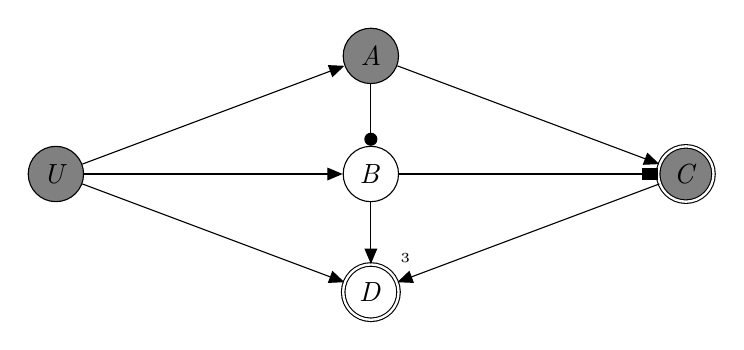
\begin{tikzpicture}
  \tikzset{neuron/.style = {shape=circle,draw,minimum size=2em,inner sep=1pt}}
    \tikzset{fireneuron/.style = {shape=circle,draw,minimum size=2em,inner sep=1pt, fill=gray}}
        \tikzset{sneuron/.style = {shape=circle,draw,minimum size=2em,inner sep=1pt, double, double distance=0.3mm}}
    \tikzset{sfireneuron/.style = {shape=circle,draw,minimum size=2em,inner sep=1pt, fill=gray,double, double distance=0.3mm}}
  \tikzset{edge/.style = {->,> = latex'}}
  \tikzset{%
  tipA/.tip={Triangle[angle=45:6pt]},
  tipS/.tip={Square[angle=45:6pt]},
}
	\node[fireneuron] (U) at (0,1.5) {$\mathit{U}$};
	\node[fireneuron] (A) at (4,3) {$\mathit{A}$};
	\node[neuron] (B) at (4,1.5) {$\mathit{B}$};
	\node[sfireneuron] (C) at (8,1.5) {$\mathit{C}$};
	\node[sneuron] (D)[label=above right:{\tiny $3$}] at (4,0) {$\mathit{D}$};
	
    \foreach \from/\to in {A/B}
    \path[-*](\from) edge node [above]{} (\to);
    
    \foreach \from/\to in {U/A, U/B, U/D, A/C, B/D, C/D}
    \path[-tipA](\from) edge node [above]{} (\to);
    
        \foreach \from/\to in {B/C}
    \path[-tipS](\from) edge node [above]{} (\to);

\end{tikzpicture}
\end{center}

The structure depicted below is a neuron diagram. $U$ is an exogenous neuron, while all other are endogenous.
$A$ and $B$ fire on a single stimuli, $C$ requires two and $D$ needs $3$ stimuli. 
Since $U$ is active, and is connected with $A$ through a stimulating edge $A$ receives a single stimuli, which in this case is sufficient for $A$ to fire.
Now, with $A$ being active, $B$ being connected to $A$ via an inhibiting edge can not be active, even though it received a stimuli from $U$.
$C$ receives one stimuli from $A$ and another from $B$, as it is connected via a stimulating edge to the prior and a negating one to latter.
Finally, with $U$ and $C$ being the only stimulants for $D$ the necessary threshold is not reached. Hence, $D$ is not active.\bigskip

Although not necessary in this work it may be of interest that \cite{erwig2010causal} properly formalised (and generalised) neuron diagrams. To do so they destination between \emph{neuron graphs} capturing an abstract neuron structure and \emph{neuron diagrams} representing the execution of neuron graphs for some set of inputs. For the subsequent definitions, let $\mathbb{F}_{\mathbb{B}}^{k,m}:= \{f \mid f:\mathbb{B}^k\to \mathbb{B}^m\}$ be the set of functions mapping $k$ boolean inputs to $m$ boolean outputs. 
Let $\cbinfoos := \bigcup_{k>0} \mathbb{F}_{\mathbb{B}}^{k,1}$ be the set of all boolean functions. 
\begin{definition}
A \emph{neuron graph} is a directed acyclic graph $\ngraph:=(\cvars, \crel, \cfoos, \pi)$, where $\cvars$ is the set of neurons and can be partitioned into endogenous variables $\cenvars$ and exogenous variables $\cexvars$; $\crel$ is a set of edges; 
 $\cfoos:=\{ F_v \mid \forall v \in \cenvars \; F_v : \cbinfoos^{\gtdegpred(v)} \to \mathbb{B} \}$ is a set of boolean functions;  for $v \in \cvars$ let $\pi(v):= (v_1,\dots, v_n) $ an ordering of $\gtpred(v)$.
%$\sigma_{\cenvars} : \cenvars \to \cbinfoos$ maps every endogenous variable to an appropriate boolean function, i.e. for every $v \in \cenvars$ one has $\sigma_{\cenvars}(v): \cbinfoos^{\gtdegpred(v)} \to \mathbb{B}$.
\end{definition}
Moreover, from this one can build a neuron diagram by taking a neuron graph and providing an assignment of the exogenous variables.
\begin{definition}
Let $\ngraph:=(\cvars, \crel, \cfoos, \pi)$ be a neuron graph, then $\ndiagram:= (\ngraph,\sigma)$ is a \emph{neuron diagram} and 
$\sigma : \cexvars \to \mathbb{B}$ being an assignment mapping exogenous variables to binary values.
%$\sigma :=\{ \sigma_v \mid \forall v \in \cexvars \;  \sigma_v \in \cbinfoos^{0,1}\}$ being a set of constant binary functions.
\end{definition}
To evaluate such a neuron diagram, a firing semantic is required. Intuitively, an endogenous neuron $v$ fires, if and only if the assigned boolean function evaluates to $1$ given the values of its predecessors ordered based on the ordering $\pi(v)$. Being assigned a constant function and having no predecessors, this recursive process ends at an exogenous node.
\begin{definition}
Let $\ndiagram:=(\ngraph,\sigma) $ be a neuron diagram, then $\interi$ is defined such that $\forall v \in \cvars$ and for $\pi(v)=(v_1, \dots, v_n)$
\begin{equation*}
\interi(v):= 
\begin{cases}
\sigma(v) & \quad \text{if} \; v \in \cexvars \\
F_v(\mathcal{I}(v_1), \dots , \mathcal{I}(v_n)) & \quad \text{if} \; v \in \cenvars
\end{cases}
\end{equation*}
(As a shorthand let $\interi(v):= \sigma_v(\mathcal{I}(v_1), \dots , \mathcal{I}(v_n))$.)
\end{definition}
This formalisation is of note, as it was used in \parencite{erwig2010causal} to create of yet another definition of token causality, which unfortunately was not captured by the methodology outlined in Chapter \ref{ch:literature_review}. 


\section{Approaches to Causation}
\label{sec:causation:approaches_to_causation}
%
%Before venturing forward into the analysing some of the many formalisms concerned with the notion of causality, a small detour through the philosophical neighbourhood of the literature landscape is necessary. 
%That is, the notion of causality has enchanted humanity since the inception of philosophy, thus it would be criminally negligent to gloss over centuries of discussion and enquiry.  
%Especially, since an investigation, even a small one, into the various traditions and approaches to causation in the philosophical literature provides additional context for the more computationally minded approaches discussed in 
%Chapter \ref{ch:comp_causality}. In this particular case, it serves as a foundation from which the fist classification scheme for formalisms is erected. 
%Moreover, when discussing (mostly) rigorously defined formalisms one needs a measure of aptitude.  Unfortunately, as of now it seems that the best method for assessing the capabilities of a formalism is by running it against an array of examples, each trying to cover some pitfall of causal reasoning. In Chapter \ref{ch:comp_causality}, those examples will be used as a second classification scheme. 
%Therefore, the chapter will be structured as follows. Section \ref{sec:causation:approaches_to_causation} relies heavily on \cite{beebee2009oxford} and provides a brief overview over the history of and the approaches to causation from a philosophical point of view. Section \ref{sec:causation:examples} is presents a collection of examples used to capture the peculiarities of human (actual) causal inference and discusses their relationships. 
%Finally, Section \ref{sec:causation:classify_causation} proposed a schemata for classifying formalisms  with
%

According to \cite{beebee2009oxford} there are standard and alternative approaches to causation. The prior including regularity theories, counter-factual theories, probabilistic theories, causal process theories and agency interventionist theories, while the latter includes theories about causal power and capacities, an anti-reductionist approach, the field of causal modelling, an approach requiring the existence of causal mechanism and one that embraces pluralism. Moreover, in \cite{halpern2016actual} distinguishes between two separate notions of causality, i.e. type (or general) causality and token (or actual) causality. 


\subsection{Type and token causality} 
The classification of causality into type and token causality is rooted in the metaphysical distinction between types and tokens, which is used to differentiate a general sort of thing and its particular occurrence \cite{wetzel2018typetoken}.

\begin{example}[\cite{hausman2005causal}]
Consider the statement 
\begin{quote}
Rose is a rose is a rose is a rose.
\end{quote}
How many different words does this sentence have.  Depending on what one may understand as word, this sentence contains three or ten different words. In the prior, the word-types of the sentence are counted, while in the latter the word-tokens are counted. 
\end{example}

In a similar vain one can distinguish two (possibly distinct) notions of  causality. \emph{Type causality}, is concerned with forward looking statements such as ``smoking causes lung cancer'', granting their wielder some predictive capabilities. Hence, establishing type causality is often the pursuit of scientific enquiry. However, often type-causal relations do not establish a strong causal connection, but rather a causal tendency. Meaning, while smoking may cause lung cancer, it is not necessary the case that a smoker will develop lung cancer, thus one may be better suited with the statement ``smoking tends cause lung cancer''. By contrast, if one wants to establish that the act of smoking caused lung cancer in a particular person, one speaks of token causality. Meaning \emph{token causality} tries to establish a connection between events that explains a certain outcome arose, thus it tends to be backwards looking.
Unfortunately, it does not seem clear whether those two notion of causation are distinct; whether type causation is merely a generalisation token causal relations, which are assumed to be fundamental, whether token causation is merely an instantiation of type level laws, which are considered as the fundamental element; whether type and token causality are simple different expression of a singular causal relation. 
For example, as will be observed in Chapter \ref{ch:comp_causality},  Halpern defines token causality in terms of type causal statements \cite{hausman2005causal,halpern2016actual}. 


The debate of what constitutes token or type causality can be extended to variables. Within this context, there is a clear difference in considering relationships between variables and relationships between variable values.
Although debated, one can classify the prior as a type-level relation, due to the fact that variables are not particulars but properties. An argument which attributes the latter as the only token-level relation \cite{hausman2005causal}.
For example, many of the formalisms using structural equations to token capture causality according to counterfactual tradition internalise this distinction as follows.
For a given causal model of the world (see causal models XXXXX), a variable $X$ is a type-level cause of a variable $Y$, if and only if there is some state of the model for which an intervention on $X$ would change the value of $Y$. An intervention on $X$, being an external change to the value of $X$ ceteris paribus all other variables. 
Whereas, the value $x$ of $X$ is an actual cause for the actual value $y$ of $Y$ (wrt.\ the model), if and only if an intervention setting $X$ to $x'$ ($x \neq x$), with other variables in the model held fixed by interventions at some combination of permissible possible values, would result in $Y$ being $y'$ ($y\neq y'$). What constitutes permissible being subject of discussion and particular for each formalism \cite{Weslake2015partialtheory}.



\subsection{Traditions}




\section{Applications}







It is vital to build an adequate repository of papers upon which this survey shall draw upon. Inherent in this construction is the tension between scope and depth, as all else equal, one compromises the other. Positioning a survey on this spectrum in a justifiable manner is rather difficult. To alleviate this tension, this section is concerned with providing a broad overview over a wide arrange of formalisms, while Chapter \ref{ch:comp_causality} discusses and analysis a narrow selection of those formalisms. The objectives of this section are accomplished by systematically constructing a literature database.
This database is analysed to obtain a structural overview of the literature, allowing for an educated selection of relevant formalisms for the subsequent discussion in Chapter \ref{ch:comp_causality}.

\chapter{The Causation Literature Landscape: A rough Picture}
\chaptermark{The Causation Literature Landscape}

The primary objective of this chapter is to draw a rough picture of the literature landscape surrounding the concept of causality in the context of computer science and logic.
This includes a heuristic grouping of authors into research communities, pointers to particularly relevant researchers and most importantly a collection of publications that provide significant contributions in the quest of illuminating and formalising the enigma that is causality. Intersecting with a wide range of subjects, e.g.\ philosophy, statistics, computer science, law, natural science, social sciences and more, as well as stretching over centuries, e.g.\ being already discussed by Hume in the 18th century, inquiries into causality are have produced an incredible the wealth of literature. Hence, to remain within a reasonable scope, it is of utmost importance to rely on a properly defined methodology and on a suitable set heuristics, to navigate this vast ocean of literature.
That is, Section \ref{sec:methodology} will provide a detailed characterisation of the publication collection process, as well as introduce and justify the methods used to identify relevant literature and their authors among the collected publications. The results of this voyage are then discussed in Section \ref{sec:results}.

%
%
%That is, by analysing the citation relationship stored in the constructed database (see Subsection \ref{subsec:database}) one can obtain a macro level view of the literature landscape and the communities within. In particular, the use of centrality measures will allow for the identification of important vertices, i.e. authors and publications, while the the application of a community detection algorithm 
%will be used to identify clusters of cooperating researches and clusters of publication based on the citation relation.
% \parencite{meho2007rise,mingers2015review,leydesdorff2012scientometrics}.
% 
%In Section \ref{sec:methodology} the methodology underlying the collection, storage and analysis of data related to publications discussing causality will be discussed. 



\section{Methodology}
\label{sec:methodology}
This section provides a detailed description of the methodology used to identify, collect and analyse the computer science, logic and philosophy literature surrounding causality. Firstly, data collection. The data, i.e.\ publications, are collected using a snowball search strategy. This requires a detailed characterisation of the set of publications from which snowball steps are conducted, as well as an adequate description of how and when those steps are employed. This information is provided in Subsection \ref{subsec:data_collection}. 
Moreover, this subsection provides a detailed description of the publicly available database used to store the meta information of the collected publications. The purpose of which is to provide other researches access to the constructed snapshot of the literature and to enhance transparency. Lastly, the methods used for the analysis of the collected data are discussed in Subsection \ref{subsec:data_analysis}. 

\subsection{Data Collection}
\label{subsec:data_collection}
The methodology underlying this systematic literature review employs a snowball search strategy. 
In general, according to \parencite{wohlin2014guidelines} any snowball search strategy should start by characterising an appropriate initial set of publications, i.e.\ the start set, which is then iteratively expanded by either forward or backward snowballing until a desirable final set of publications is obtained.
Furthermore, according to \parencite{wohlin2014guidelines} this start set should satisfy the following criteria.
\begin{itemize}
\item The start set should cover a diversity of communities.
\item The number of papers in the start set should not be too small.
\item The number of papers in the start set should not be too big.
\item The start set should cover several different publishers, years and authors.
\item The start set ought to be formulated from keywords (and their synonyms) in the research question.
\end{itemize}
Moreover, they state that any snowball step on a given set of publications consists of both forward and backward snowballing.
The latter, adds all relevant references from all unprocessed publications to the set of publications. By contrast, the prior leverages modern technologies, such as \href{https://scholar.google.at/}{Google Scholar} to identify every relevant publication that references any unprocessed publication in the provided set \parencite{wohlin2014guidelines}.



Using this as a template, the actual methodology is constructed as follows. Firstly, the objectives that ought to be satisfied by the snowball search strategy are made explicit. In this particular case those objectives are to
\begin{itemize}
\item focus on token causality publications;
\item focus primarily on publications related to computer science and artificial intelligence;
\item focus secondarily on publications related to philosophy or law;
\item focus on publication that approach causality with sufficient formality;
\item focus on logic and rule based approaches to causality;
%\item focus on publications emerging from the fields, computer science, logic, philosophy or law, i.e.\ avoid publications emerging from the machine learning community;
\item focus on the recent literature, i.e.\ publications between 2010 and (early) 2020.
\end{itemize}
Being a snowball search, the growth rate of the publications to consider is exponential. Hence, to serve the outlined objectives it is vital to construct a starting set that provides a sufficient strong directive.
Since the primary focus is to remain within the greater context of computer science, logic and (symbolic) artificial intelligence, the start set construction is initiated by considering all articles from  
\begin{itemize}
\item \href{https://www.journals.elsevier.com/knowledge-based-systems}{Journal Knowledge-Bases Systems} (KBS)
\item \href{https://www.journals.elsevier.com/artificial-intelligence}{Journal Artificial Intelligence} (AI)
\item \href{https://www.springer.com/journal/10506}{Journal Artificial Intelligence and Law} (AI\&Law)
\item \href{https://www.ijcai.org/}{International Joint Conferences on Artificial Intelligence Organization} (IJCAI)
\end{itemize}

that where published between 01.2017 and 3.2020. Focusing on such recent publications, should serve the recency bias established in the methodology's objectives. 
The collected publications are subsequently preprocessed using a simple key word search. That is the first necessary condition for a publication to be in the start set is 
\begin{itemize}
\item  that its title contains a string starting with the character sequence \emph{``caus''} or 
\item  its abstract contains a string starting with the character sequence \emph{``causal''}. 
\end{itemize}
Let $\xsetz$ be the subset of all collected publications, that satisfy this criteria.
To focus on logic and rule based approaches, all publications that are deemed irrelevant under closer inspection or are inaccessible will be removed. The classification as relevant is done based on a list of soft criteria. By satisfying positive criteria the publication increases its chance of being deemed relevant, satisfying negative ones decreases its chance, and criteria marked by ``$\ast$'' are necessary.
\begin{itemize}
\item[$\ast$] Does the publication discuss causality or any related concept, e.g.\ counterfactuals? 
\item[$+$] Does the publication engage with the philosophical aspects of causality?
\item[$+$] Does the publication try to formalise causality using logic (or another formal language)?
\item[$+$] Does the publication's title explicitly mention logic and/or causality?
\item[$+$] Does the publication is discuss token causality (see Section XXX)?
\item[$-$] Does the publication discuss causality in the context of machine learning?
\item[$-$] Does the publication discuss causality in a highly informal manner?
\item[$-$] Is the publication a book?
\end{itemize}

To explain the snowballing step, some general notation must be introduced. Let $\mathcal{X}$ be some set of publications.
Then $\mathcal{X}^c$ is the set of publication deemed relevant by the previously stated criteria. Furthermore, let $\mathcal{X}^{r}$ be the set of publication deemed relevant by the previously stated criteria, which are published after (and including $2010$). 
Additionally, let $\pi^-(\mathcal{X})$ be the set of accessible publications, not contained in $\mathcal{X}$, that are obtained by backward snowballing on $\mathcal{X}$. Moreover, let $\pi^+(\mathcal{X})$ be the set of accessible publications, are not contained in $\mathcal{X}$, which are obtained by forward snowballing on $\mathcal{X}$ using Google Scholar between 16.04.2020 until 20.04.2020.

Utilising this notation, let $\xsetz^r$ be the start set of this snowball search. 
From there, a variation of forwards- and backwards-snowballing steps are applied to construct the set $\xset$. That is, 
%
%Let the final start set be denoted with $\psetz$ and let $\npsetz:=\tpsetz \setminus \psetz $, i.e.\ all publications discarded in Step 3 that were deemed relevant in Step 2. 
%Using $\psetz$ the actual paper repository $\pset$ is constructed by using a varied combination of forward and backward snowballing steps.
%Moreover, for some Step $x$,
%%$x \in \{ \mathit{+1}, \mathit{+1-1}, \mathit{+2}, \mathit{+2-1}, \mathit{-1}, \mathit{-2}\}$, l
%let $\tpset_x$ be the set of all publications obtained by snowballing on a previous set $\tpset_y$. Then $\pset_x \subseteq \tpset_x$ is the set of all publications considered relevant according to the criteria established in Step 3 and $\npset_x := \tpset_x \setminus \pset_x$ is the set of publications from $\tpset_x$ that are deemed irrelevant. 
\begin{itemize}
\item $\xsetb:=\pi^-(\xsetz^r)$;
\item $\xsetbb:= \pi^-(\xsetb^r)=\pi^-(\pi^-(\xsetz^r)^r)$;
\item $\xsetf:= \pi^+(\xsetz^r)$;
\item $\xsetfb:= \pi^-(\xsetf^r)=\pi^-(\pi^+(\xsetz^r)^r)$;
\item $\xsetff:= \pi^+(\xsetf^r)= \pi^+(\pi^+(\xsetz^r)^r)$;
\item $\xsetffb:= \pi^-(\xsetff^r)=\pi^-(\pi^+(\pi^+(\xsetz^r)^r)^r)$;
\end{itemize}
and finally, $\xset := \xsetz \cup \xsetb \cup \xsetbb  \cup \xsetf  \cup \xsetfb  \cup \xsetff \cup \xsetffb$.


%
%\begin{itemize}
%\item $\pset_1:= \psetz \cup \psetb$; $\tpsetb$ contains all publications that are not in $\psetz$, which were obtained by backwards snowballing on all accessible articles in $\psetz$; 
%\item $\pset_2:= \pset_1 \cup \psetbb$; $\tpsetbb$ contains all publications that are not in $\pset_1$, which were obtained by backwards snowballing on all accessible articles in $\psetb$ published after (and including) $2010$.
%\item $\pset_3:= \pset_2 \cup \psetf$; $\tpsetf$ contains all publications that are not in $\pset_2$, which were obtained by forwards snowballing\footnote{using Google Scholar on the 16.04.2020} on all articles in $\psetz$.
%\item $\pset_4:= \pset_3 \cup \psetfb$; $\tpsetfb$ contains all publications that are not in $\pset_3$, which were obtained by backwards snowballing on all articles in $\psetf$.
%\item $\pset_5:= \pset_4 \cup \psetff$; $\tpsetff$ contains all publications that are not in $\pset_4$, which were obtained by forwards snowballing on all articles in $\psetf$.
%\item $\pset:= \pset_5 \cup \psetffb$; $\tpsetffb$ contains all publications that are not in $\pset_5$, which were obtained by backwards snowballing on all articles in $\psetff$.
%\end{itemize}
% XXXX paperb vs publication straiten out.


Before moving on, a small discussion about the single most undesirable property of this process. That is, in an ideal world the methodology would provide a perfectly reproducible algorithm that reliably and deterministically produces the same set of publications on each execution.
Unfortunately, this property can not be satisfied by the constructed methodology, as any employment of forward snowballing introduces variability into the system. Considering the importance of forward snowballing to identify the most recent literature, foregoing the application of this tool in the construction of $\xset$ would not have been feasible. Having already parted with this desirable property, conditions that further prohibit reproducibility, i.e. the soft categorisation of relevance and the removal of inaccessible publications, could be added without concerns.



The dataset constructed using this methodology is publicly available (including a Python script for easy access). It is stored in a \href{https://www.sqlite.org/index.html}{SQLite-database} and was constructed using \href{https://www.sqlalchemy.org}{SQLAlchemy}.
This database can store publications, authors, venues and tags. Its structure is depicted in Figure \ref{fig:er-diagram-publication-db} as an ER-diagram using Chen notation \parencite{chen1976entity}.

\begin{figure}[h!]
\begin{center}
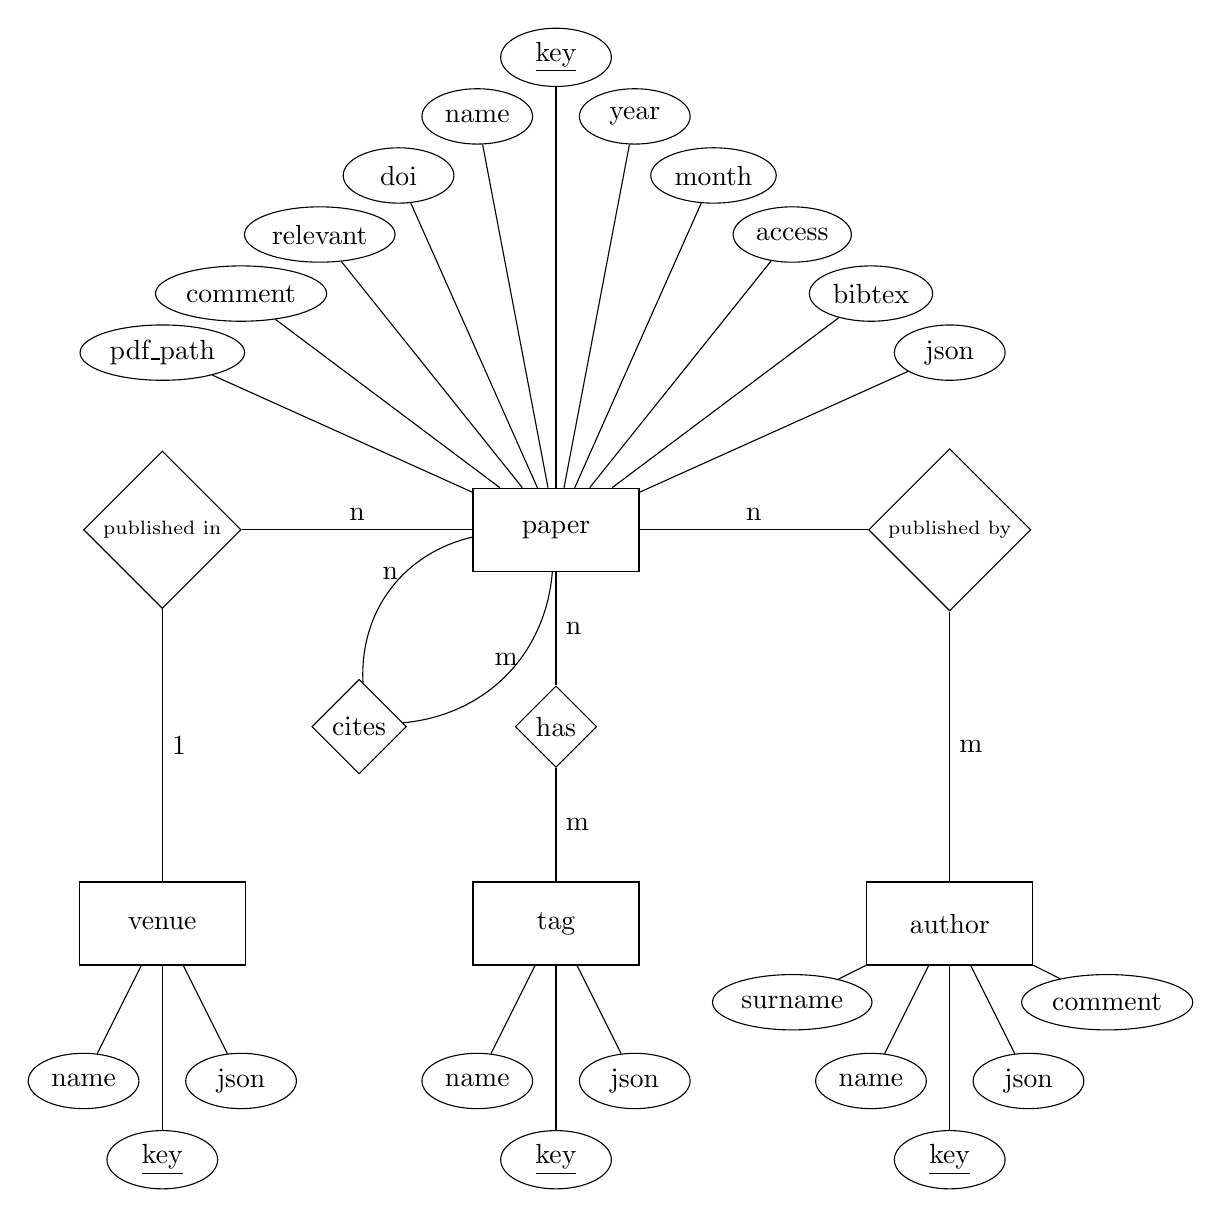
\begin{tikzpicture}
  \tikzset{entity/.style = {shape=rectangle,draw,minimum size=3em,minimum width=6em,inner sep=5pt}}
  \tikzset{relation/.style = {shape=diamond,draw,minimum size=2em,inner sep=2pt}}
  \tikzset{attribute/.style = {shape=ellipse,draw,minimum size=2em,minimum width=4em,inner sep=2pt}}

	
	\node[entity] (P) at (5,9) {paper};
	\node[entity] (T) at (5,4) {tag};
	\node[entity] (V) at (0,4) {venue};
	\node[entity] (A) at (10,4) {author};

	\node[relation] (PT) at (5,6.5) {has};
	\node[relation] (PV) at (0,9) {\scriptsize published in};
	\node[relation] (PA) at (10,9) {\scriptsize published by};
	\node[relation] (PP) at (2.5,6.5) {cites};
	
	
	\node[attribute] (Vname) at (-1,2) {name};
	\node[attribute] (Vkey) at (0,1) {\underline{key}};
	\node[attribute] (Vjson) at (1,2) {json};
	
		
	\node[attribute] (Tname) at (4,2) {name};
	\node[attribute] (Tkey) at (5,1) {\underline{key}};
	\node[attribute] (Tjson) at (6,2) {json};
	
			\node[attribute] (Asurname) at (8,3) {surname};
		\node[attribute] (Aname) at (9,2) {name};
	\node[attribute] (Akey) at (10,1) {\underline{key}};
	\node[attribute] (Ajson) at (11,2) {json};
			\node[attribute] (Acomment) at (12,3) {comment};
			
			
	\node[attribute] (Pkey) at (5,15) {\underline{key}};
	\node[attribute] (Pname) at (4,14.25) {name};
	\node[attribute] (Pyear) at (6,14.25) {year};
		\node[attribute] (Pdoi) at (3,13.5) {doi};
	\node[attribute] (Pmonth) at (7,13.5) {month};
			\node[attribute] (Prelevant) at (2,12.75) {relevant};
	\node[attribute] (Paccess) at (8,12.75) {access};
	
				\node[attribute] (Pcomment) at (1,12) {comment};
	\node[attribute] (Pbibtex) at (9,12) {bibtex};
	
					\node[attribute] (Ppdf) at (0,11.25) {pdf\_path};
	\node[attribute] (Pjson) at (10,11.25) {json};
	
	
	

    \path[-](P) edge node [above]{n} (PA);
      \path[-](PA) edge node [right]{m} (A);
      
          \path[-](P) edge node [right]{n} (PT);
      \path[-](PT) edge node [right]{m} (T);
      
          \path[-](P) edge node [above]{n} (PV);
      \path[-](PV) edge node [right]{1} (V);



	\path[-](P) edge [bend right=40] node [above]{n} (PP);
   \path[-](PP) edge [bend right=40] node [above]{m} (P);
   
       \foreach \from/\to in {V/Vkey, V/Vname, V/Vjson, T/Tkey, T/Tname, T/Tjson,  A/Asurname, A/Acomment, A/Akey, A/Aname, A/Ajson,
       P/Pkey, P/Pname, P/Pyear, P/Pdoi, P/Pmonth, P/Prelevant, P/Paccess, P/Pcomment, P/Pbibtex, P/Ppdf, P/Pjson}
    \path[-](\from) edge node [above]{} (\to);
    
    


\end{tikzpicture}
\end{center}
\caption{ER-Diagram of the database.}
\label{fig:er-diagram-publication-db}
\end{figure}



The table ``Venue'' stores platforms that publish research, e.g.\ journals such as AI or conferences such as IJCAI. This table is rather sparse, having only a column for the names of the venues and a column reserved for a \href{https://www.json.org/json-en.html}{JSON-string} in case additional data must be stored. 
Similar in structure is the ``Tag'' table. It's intended purpose is to store tags that can be used to further categorise publications, e.g.\ they are used to identify which publications were added to the database at which snowballing step.
Slightly more complex is the ``Author'' table, which contains an additional column for surnames, as well as a column reserved for comments. The last column allows one to differentiate authors with identical name. 
By far the most extensive one is the Table ``Paper''. 
Firstly, it provides columns for basic information such as the title, the DOI, the publication year and month, as well as its \BibTeX-string.
Moreover, it contains columns to track whether a publication was accessible and whether it is deemed relevant. 
Furthermore, for easy access there exists also a column storing the local path to the pdf-file of the publication.
Lastly, columns for comments and for storing additional data in JSON-format are provided as well.


Those table relate to each other as follows. 
Firstly, the table ``Venue'' is connected to the table ``Paper'' via an 1:n-relation.
Secondly, the ``Author''- and the ``Paper''-table are in an m:n-relation. The same holds true for the ``Tag''- and the ``Paper''-table.
Thirdly, to store the citation relations between publications, the table ``Paper'' is in an m:n-relation with itself.

During the data collection, publications will be assigned one of seven tags. Those are \texttt{0}, \texttt{-1}, \texttt{-2}, \texttt{+1}, \texttt{+1-1} \texttt{+2}  and \texttt{+2-1} and indicate membership to the respective sets constructed during the snowballing process.



%\begin{tikzpicture}[auto,node distance=1cm]

  % Create an entity with ID node1, label "Fancy Node 1".
  % Default for children (ie. attributes) is to be a tree "growing up"
  % and having a distance of 3cm.
  %
  % 2 of these attributes do so, the 3rd's positioning is overridden.
%  \node[entity] (AT) {author}
%    [grow=up,sibling distance=3cm]
%    child {node[attribute] {name}}
%    child {node[attribute] {surname}}
%     child {node[attribute] {comment}}
%     child {node[attribute] {json}};
%    
%     \node[entity] (VT) {venue}
%    [grow=up,sibling distance=3cm]
%    child {node[attribute] {name}}
%     child {node[attribute] {json}};
%     
%     
%          \node[entity] (TT) {tag}
%    [grow=up,sibling distance=3cm]
%    child {node[attribute] {name}}
%     child {node[attribute] {json}};
%     
%%   
%          \node[entity] (PT) {paper}
%    [grow=up,sibling distance=3cm]
%    child {node[attribute] {name}}
%    child {node[attribute] {doi}}
%    child {node[attribute] {year}}
%    child {node[attribute] {month}}
%    child {node[attribute] {relevant}}
%    child  {node[attribute] {access}}
%    child {node[attribute] {comment}}
%    child  {node[attribute] {bibtex}}
%    child  {node[attribute] {pdf\_path}}
%     child {node[attribute] {json}};
%     
     
%  % Now place a relation (ID=rel1)
%  \node[relationship] (rel1) [below right = of node1] {Relation 1};
%  % Now the 2nd entity (ID=rel2)
%  \node[entity] (node2) [above right = of rel1]	{Fancy Node 2};
%  % Draw an edge between rel1 and node1; rel1 and node2
%  \path (rel1) edge node {1-\(m\)} (node1)
%    edge	 node {\(n\)-\(m\)}	(node2);
%\end{tikzpicture}


\subsection{Data Analysis Methods}
\label{subsec:data_analysis}
The data analysis will proceed according to the following steps. The first, is the construction of several graphs using the stored citation relation and the co-authorship relation. This is followed by a heuristic detection of research communities obtained through the application of a community detection algorithm. Following this, a combination of centrality measures and publication counts will be used to identify the most prominent authors in this field. Lastly, a similar approach will be employed to identify it's most significant publications.

Considering the collected data it is possible to construct several graph structures.
The first two are constructed such that their vertices represent publications and their edges correspond to citations, i.e.\ each edge $(A,B)$ implies that there exists a publication $A$ that references another publication $B$. The only difference between those two graphs, called $\tgraph$ and $\pgraph$, is that the vertex set of $\tgraph$ is $\xset$ and that of $\pgraph$ is $\xset^r$, i.e.\ it contains only those publication that were deemed relevant and that have been published from 2010 onwards.
By construction, both of them are directed\footnote{The graph in question does contain cycles. This is due to the fact that sometimes not yet publicised works are cited, which contain a reference back to the original publication.}
Of particular relevance is $\pgraph$, also called ``publication graph'', because it serves as the bedrock of all subsequent analysis. That is, it is used to construct a set of important publications from which all formal languages, definition and examples discussed in subsequent chapters are extracted.
While it is tempting to use $\tgraph$ for such a task, succumbing it is ill advised. Because, by construction, only the publications in $\pset$ that were published after (and including) $2010$ contain a complete mapping of their citations. Hence, using $\tgraph$ for such an important task is undesirable, as this would obviously distorts the relative relevance between the analysed publications. However, a quick analysis of $\tgraph$ will be presented to provide a rough understanding of the literature published before 2010.
The other three graphs, encode information about the authors and the relationships between them. Starting with the ``author graph'' $\agraph$. It encodes the citations between authors, rather than between publications. Every vertex in $\agraph$ represents an author, who has at least one publication represented in $\pgraph$. Every edge in $\agraph$ between an author $A$ and an author $B$ indicates that there exists at least one publication of $A$ that cites at least one publication of $B$ (with respect to $\pgraph$), while its weight represents the frequency of this occurrence. To account for multiple citations, as well as self-referential behaviour, $\agraph$ must a be a directed, weighted graph containing loops.
The second, $\cgraph$ or ``collaboration graph'', encodes the collaborations between authors. That is, while its vertex set is identical to $\agraph$'s vertex set, an edge in $\cgraph$ between an author $A$ and an author $B$, indicates that $A$ and $B$ co-authored a publication in $\pgraph$, thus the weight of an edge represents how often they collaborated on publications in $\pgraph$. 
The last, $\acgraph$ or ``merged graph'' is simply a merger of $\agraph$ and $\cgraph$, where each undirected edge is replaced by two opposing directed edges (in the case of duplicate edges, their weights are summed up).
To summarise, $\tgraph$ and $\pgraph$ are a directed graphs; $\agraph$ and $\acgraph$ are directed, weighted graphs containing loops and $\cgraph$ is an undirected, weighted graph. 


The as a whole the constructed graphs are subjected to two different kinds of information extraction processes. The first uses the community detection algorithm to identify research communities, while the second uses a variety of centrality measures to identify important publications and authors. 
%All of which is done based on the publication count, the co-authorship and the citation relation between publications.  
Approaches leveraging such techniques fall under the term ``citation analysis''. A area of research concerned with the discovery and management of literature by analysing its references to evaluate scholarly contributions, track the flow of knowledge, study the structure of research field, etc. \parencite[p.~1-5]{zhao2015analysis}. While useful, this requires the acceptance of several assumptions. Namely,
\begin{itemize}
\item citation of a document implies use of that document by the citing author;
\item citation of a document (author, journal, etc.) reflects the merit (quality, significance, impact);
\item citations are made to the best possible works;
\item a cited document is related in content to the citing document;
\item all citations are equal.
\end{itemize}
While accepting those rather strong assumptions is problematic, many of which were already violated by this text, additional concerns with this technique arise when one also considers that there can be various problems in the data, e.g.\ errors, self-citations or multiple authors. However, due to the fact that the those techniques are only used in a rudimentary manner to provide a starting point for the subsequent research, a proper justification of the applicability of those assumptions with respect to the given data will be omitted. However to satiate possible curiosity, please consider \parencite{smith1981citation} for detailed discussion about the validity of those assumption.



Firstly, the detection of communities. For the purposes of this work, a groups of researches is classified as a community (with respect to their work on causation), if the group is of size greater than two and if the group produced more than two relevant publications. This analysis approach should provide a rough estimate of the research clusters in the literature based on the information encoded in $\acgraph$. 
The community detection itself is accomplished using an algorithm published in \parencite{rosvall2008maps}. 
This particular algorithm uses an information theoretic approach to lay bare the community structure in an directed weighted graph.
Hence, if one excludes self-referential behaviour, the same algorithm can be used on any graph up for analysis, thus it is well suited for $\acgraph$. Furthermore, \parencite{rosvall2008maps} introduces their algorithm by studying a citation graph.
Demonstrating the suitability of the algorithm for such tasks in the process. As the results obtain through community detection are less significant for the subsequent chapters, please consult \parencite{rosvall2008maps} for further discussion and additional details. 
Nevertheless, to identify relevant communities the following proceeder will be used. 
Firstly, $\acgraph$ will be cleared from all loops. Secondly, all authors that are only cited or that only cite, with respect to the collected data, are removed. 
Thirdly, the community detection algorithm is applied to the graph. Lastly, all communities are ranked based on the average number of relevant publications per author. Hence, providing the possibility for smaller communities to get some spotlight as well.


The primary technique used in this work to assess the importance of a vertex in a graph, relies on the use of centrality measures. Being significant for the work in subsequent chapters, the discussion of such measures warrens a more detailed discussion as compared to community detection part. In general, those centrality measures are used to rank vertices based on some notion of importance. In particular, they can be used to understand diffusion processes, assess an individuals risk of infection or explain the influence of a 
person in a social network \parencite{bloch2019centrality}. According to \parencite{del2011centrality} degree, closeness and betweenness centralities are the most popular ones. Additionally, there exists a family of centralities that is closely tied to field of spectral graph theory (see \parencite{spielman2012spectral}), as those centralities use eigenvalues and eigenvectors in their computation. This includes measures such as the eigenvector centrality, alpha centrality, page rank and Katz-Bonacich centrality  \parencite{bloch2019centrality}. 



The following, provides a brief intuition about some of the mentioned centrality measures and is compiled from information found in \parencite{segarra2015stability,del2011centrality,bloch2019centrality,bonacich2001eigenvector,page1999pagerank}.
The degree centrality is a local measure of importance based on the degree of a vertex. In the case of a weighted graph, the weighted degree of a vertex is taken for this measurement, thus implying that the weight of an edge must reflect some notion of similarity. That is, a higher weight implies a stronger connection, e.g.\ number of interactions. If one is confronted with an directed graph, the degree centrality dissolves into an in- and out-degree centrality.
Although it can be used to assess the ``popularity'' of a vertex, due to its locality it neglects the remaining structure of the graph. 
The closeness centrality is computed using the sum of all shortest path lengths. Hence, it is a measure for assessing the importance of a vertex based on how quick such a vertex can reach every other vertex. 
Moreover, this implies that edge weights must indicated a notion of dissimilarity, e.g.\ distance between vertices. Unfortunately, this measure requires the graph to be strongly connected. Hence, it is not suitable for directed graphs in general.  
The betweenness centrality gives higher values to vertices that are part of many shortest paths between pairs of vertices. Meaning it attempts to assess the importance of a vertex based how vital a vertex is for the flow of information between the other vertices in the graph. As this centrality builds upon the notion of a shortest path, it requires the weights of a graph to represent a dissimilarity between vertices. However, a benefit of this centrality is that it is suitable for both directed and undirected graphs.
The eigenvector centrality is similar to the degree centrality, as it assess the importance of a vertex based on the number of neighbours, thus it requires weights to denote similarities. However, it differs in the evaluation of those neighbours, determining the importance of a vertex based in the importance of the vertices in its neighbourhood. That is, the eigenvector centrality is computed by assuming that the centrality of a vertex is proportional to the sum of eigenvector centralities of the vertex's neighbours. Hence, it is a self-referential process. Unfortunately, common implementations requires graphs to be undirected and connected. 
The  alpha centrality is a generalisation of the Eigenvector centrality for directed graphs. The idea behind this centrality is that it assumes that a vertex has some exogenously defined start value. The Katz-Bonacich centrality generalises the Eigenvector centrality by reducing the importance of distant vertices. 
Page Rank relativises the centrality score passed on by a vertex, based on the number if neighbours. Hence, a vertex having a directed edge to an important vertex must not necessarily have a high importance itself, e.g.\ a webpage linking to an important webpage must not necessarily be important itself. Furthermore, to ensure sensible results in directed graphs, dead ends are avoided by jumping to a random vertex instead.


Each of those measures allow for a separate ranking of publications and authors. 
However, a blind application of those methods would neglect the structure of the graphs and thus could lead to erroneous results. Hence, some additional care must be given and some slight adjustments to the graphs are required.
In the case of $\pgraph$, one is faced with an directed (and not strongly connected) graph. Therefore, the closeness or eigenvector centrality are ill suited for application on this graph.
Furthermore, the degree centrality is obviously applicable. However, it decomposes into two separate measures. Additionally, the regular degree centrality will be used as well. That is, in the context of this particular dataset, the regular degree distribution actually provides a rough compromise between the recency bias of the out-degree, as well as the conservative tendencies associated with the in-degree measure (this can be observed in Figure \ref{fig:pgraph-avgr_degree_year}). Hence, the undirected degree measure will be used as well. Unfortunately, due to their locality degree centralities provide a rather limiting picture, thus in an attempt to compensate for this shortcoming an alternative to the eigenvector centrality, namely page rank, is used. Although it is somewhat unusual to use this algorithm for citation graphs, this approach is not unheard of, see \parencite{ding2009pagerank,ma2008bringing,chen2007finding,maslov2008promise,nykl2014pagerank} for an in-depth discussions. One particular benefit of determining the importance of a publication in such a manner, is that under Page Rank simply referencing an important publication, does not indicate a publications own importance. The last remaining common centrality measure, the Betweenness centrality, can and thus will be applied. Providing yet another dimension for selecting publications. 


In the case of $\agraph$, one is faced with a directed, weighted graph containing loops. Hence, modifications to the graph are required. Firstly, while included for the sake of completion in the graph $\agraph$, it seems sensible to discount self-referential behaviour for the ranking. Secondly, all centrality measures used in the ranking of publications
can accommodate weights in their assessment. However, the Betweenness Centrality requires the weight of an edge to express dissimilarity, thus it is necessary to convert the weights such that they express dissimilarity rather than similarity between vertices (see \cite[p.~13]{runkler2012data}). Moreover, in addition to the centralities it is reasonable to include the number of publications (in the examined field) as an additional measure. 




\section{Analysis}
\label{sec:results}
This section starts by discussing the data collection process and by describing the collected data through the performance of a rudimentary quantitative analysis. All of which is discussed in Subsection \ref{subsec:basic_data_analysis}. 
The subsequent subsection, i.e.\ Subsection \ref{subsec:communities_authors_publications}, attempts to draw a rough picture of the literature landscape, by utilising the techniques outlined in Subsection \ref{subsec:data_analysis}. 



\subsection{Data Preparation and Basic Analysis}
\label{subsec:basic_data_analysis}
This subsection quantitatively describes the data collection process, while highlighting detected mistakes as well as deviations from the constructed methodology.    
Moreover, this is followed by a brief and offensively basic investigation into the collected data. Am analysis that is subsequently expanded upon, by presenting some key properties of the graphs $\tgraph$, $\pgraph$, $\agraph$, $\cgraph$ and $\acgraph$.



Using the outlined methodology the following literature database was constructed. 
By collecting all publications from the venues
Journal Artificial Intelligence (AI), Journal Artificial Intelligence and Law (AI\&Law), International Joint Conferences on Artificial Intelligence Organization (IJCAI) and Knowledge-Bases Systems (KBS) that where published between 01.2017 and 3.2020 one obtains a set containing $4223$ publications. To be precise, AI contributed $267$ publications, by contrast  AI\&Law provided only $60$. Furthermore, from KBS a total of $1281$ publications could be obtain, while the majority of publications, i.e.\ $2615$, was sourced from IJCAI.
After applying the keyword based filter, the set of publications, i.e.\ $\xsetz$ up for consideration is reduced to a meagre $37$.\footnote{\parencite{van2019separators,verheij2017proof,chen2019judicial,neil2019modelling,li2019context,lu2018mining,zhang2018collective,
constantinou2017towards,liang2017evaluation,zhang2017characterizing,mu2018measuring,kronegger2019backdoors,hyttinen2017core,
zhang2017transfer,zhang2017causal,liu2017cause,summerville2017charda,zhang2016causal,albrecht2016exploiting,chai2018language,
bochman2018actual,ibeling2018conditional,laurent2018counterfactual,chikahara2018causal,zhang2017achieving,backstrom2018novel,
jaber2018graphical,sridhar2018scalable,wenjuan2018mixed,xu2019achieving,zhang2019asp,Cai2019CausalDW,Sridhar2019EstimatingCE,
xie2019boosting,hassanzadeh2019answering,shankar2019three,Liepina2019ArguingAC}}

After closer investigation, the publications deemed relevant according to the specified criteria are 
\begin{itemize}
\item Proof with and without probabilities \parencite{verheij2017proof};
\item Characterizing causal action theories and their implementations in answer set programming\footnote{Since \parencite{zhang2017characterizing} was not accessible ``Characterizing causal action theories and their implementations in answer set programming: Action languages b, c, and beyond" \parencite{zhang2015characterizing} will be used for the snowballing step. This departure from the methodology, is justified due to its initially high reprieved relevancy.}; \parencite{zhang2017characterizing};
\item Actual Causality in a Logical Setting \parencite{bochman2018actual};
\item On the conditional logic of simulation models \parencite{ibeling2018conditional};
\item  Counterfactual Resimulation for Causal Analysis of Rule-Based Models \parencite{laurent2018counterfactual};
\item Scalable Probabilistic Causal Structure Discovery \parencite{sridhar2018scalable};
\item  ASP-based discovery of semi-Markovian causal models under weaker assumptions \parencite{zhang2019asp};
\item Arguing about causes in law: a semi-formal framework for causal arguments \parencite{Liepina2019ArguingAC}.
\end{itemize}
Hence, $\xsetz^c$ contains only $8$ publications.
Executing the described snowballing steps on the start set, one obtains a total of $872$ publications. Out of which only $294$ (around $34 \%$) are categorised as relevant. 
As depicted in Figure \ref{fig:pgraph-relevant_publications_per_step}, this can be made more precise. Meaning that $\xsetb$ obtained by performing backwards snowballing on $\xsetz^r$, contains $204$ publications out of which only $79$ are relevant. The second backwards snowballing step, i.e. $\pi^-(\xsetb^r)$, provided a total of $486$ publications with $165$ being relevant. The set $\psetf$ contains $30$ publications collected by forward snowballing on $\xsetz^r$. Performing a backward snowballing step on $\psetf^r$ generates $\psetfb$ which contains $63$ publications from which $25$ are deemed relevant. The second forward snowballing step, i.e. $\pi^+(\xsetf^r)$, produces $\xsetff$ resulting in an additional $7$ publications with only $3$ relevant ones among them. Lastly, by performing a final backward snowballing step on $\xsetff^r$, $45$ new publications are discovered increasing the number of relevant publications by another $7$.  



\begin{figure}[h!]
\includegraphics[width=\textwidth]{relevant_publications_per_step.png}
\caption{Number of publications and relevant publications added during each snowballing step.
(From left to right $\xset_x^c/\xset_x$: $8/37$, $79/204$, $165/486$, $7/30$, $25/63$, $3/7$, $7/45$)}
\label{fig:pgraph-relevant_publications_per_step}
\end{figure}




Although great effort was taken to make the data collection sufficiently accurate. Some mistakes were discovered the data collection was already completed.
Particularly of note is that there are two publications titled ``Causes and explanations: a structural-model approach: part i: causes'' by the same authors, i.e.\ \parencite{halpern2001causes} and \parencite{halpern2005causes}.
During the data collection process those two publication were unfortunately conflated. Fortunately, the similarities between those two publications, the latter provides an updated to definition presented in the prior, relativise this mistake.


From the meta-data of the publications alone, one is able to observe the contributions to this field over the years. That is, given the publication dates of the literature collected in $\xset^c$ it is possible to construct Figure \ref{fig:pgraph-relevant_publications_per_year}, which depicts the distribution of number of publications (in $\xset^c$) per year across the past 50 years.
Furthermore, according to the data collected, the decade between $2000$ and $2010$ was the most productive period, i.e.\ $\pset$ contains $73$ publications before 2000, $114$ between 2000 and 2010 and $107$ publications from 2010 onwards. Additionally, it can be observed that 2004, 2007 and 2009 were the most productive years over all. Containing notable publications such as 
``Nonmonotonic Causal Theories'' \parencite{giunchiglia2004nonmonotonic}, ``Causes and Norms'' \parencite{hitchcock2009cause}, ``Prevention, Preemption, and the Principle of Sufficient Reason'' \parencite{hitchcock2007prevention}, ``Two Concepts of Causation'' \parencite{hall2004two} and ``Structural Equations and Causation'' \parencite{hall2007structural}
\footnote{discussing and using formalisms such as Neuron Diagrams, Structural Equations and some variant of McCain and Turner's Causal Logic}.


\begin{figure}[h]
\includegraphics[width=\textwidth]{relevant_publications_per_year.png}
\caption{Number of relevant publications per year (a negligible amount publications occur before 1970)}
\label{fig:pgraph-relevant_publications_per_year}
\end{figure}



Further information can be extracted by encoding the collected data as graphs. As discussed earlier, the set of publications $\xset$ and their references naturally induce a directed 
%(acyclic\footnote{The graph in question does contain cycles. This is due to the fact that sometimes not yet publicised works are cited, which contain a reference back to the original publication.}) 
graph containing 872 vertices and 2052 edges. This graph, i.e.\ $\tgraph$ can be observed in Figure \ref{fig:pgraph-whole_graph}.
Induced by the set $\xset^r$, containing publications that are both relevant and are published after (and including) $2010$, one obtains $\pgraph$ as a sub-graph of $\tgraph$.
$\pgraph$ contains only $107$ and $326$ edges and can be observed in Figure \ref{fig:pgraph-actual_graph}.
Using $\pgraph$ one can then compute $\agraph$, visible in Figure \ref{fig:agraph-actual_graph}, which contains a total of $130$ vertices and $462$ edges. As discussed this graph encodes the citations between authors and not the one between publications. Hence, it requires that its directed edges are weighted. 
To analyse the co-authorship relation one can create $\cgraph$. It is depicted in Figure \ref{fig:cgraph-actual_graph} and contains $130$ vertices and $192$ undirected, weighted, edges.
Lastly, $\acgraph$, depicted in Figure \ref{fig:acgraph-actual_graph}, is the merger of $\agraph$ and $\cgraph$, thus it contains $130$ vertices and $755$ edges. 
For a quick overview of some of their basic properties please consult Table \ref{tab:graph-stat} and Table  \ref{tab:pgraph-degree_stat}, as well as Figure \ref{fig:pgraph-degree_distr},  Figure \ref{fig:agraph-degree_distr} and  Figure \ref{fig:cgraph-degree_distr} respectively.

\begin{sidewaysfigure}[h]
\includegraphics[width=\textwidth]{whole_graph.png}
\caption{$\tgraph$ where \textcolor{start_relevant}{dark red}  (\textcolor{start_nrelevant}{dark blue}) indicates a(n) (ir)relevant publication in $\xsetz$ and \textcolor{other_relevant}{light red}  (\textcolor{other_nrelevant}{light blue}) indicates a(n) (ir)relevant publication in $\xset\setminus \xsetz$. (Isolated vertices are not depicted in this graph and edge direction is suppressed.)}
\label{fig:pgraph-whole_graph}
\end{sidewaysfigure}



%Unfortunately, only the publications in $\pset$ that were published after (and including) $2010$ contain a complete mapping of their citations. As this obviously distorts the relative relevance between the analysed publications, all other publications must be discarded from the analysis. Hence, reducing the set of considered publications to only $107$. The subgraph induced by the set containing relevant publications from the year 2010 onwards, constitutes the bedrock for the subsequent analysis and paper selection. It is named $\pgraph$ or ``Publication Graph'' and can be observed in . 

\begin{sidewaysfigure}[h!]
\includegraphics[width=\textwidth]{actual_graph.png}
\caption{The publication graph $\pgraph$, containing all relevant publications published after (and including) 2010. It consists out of $107$ vertices ($8$ are in \textcolor{cstepz}{$\xsetz^r$}; $29$ are in \textcolor{cstepb}{$\xsetb^r$};
$42$ are in \textcolor{cstepbb}{$\xsetbb^r$}; $7$ are in \textcolor{cstepf}{$\xsetf^r$}; $17$ are in \textcolor{cstepff}{$\xsetff^r$}; $3$ are in \textcolor{cstepfb}{$\xsetfb^r$}; $1$ are in \textcolor{cstepffb}{$\xsetffb^r$}) and $326$ edges. The vertex size correlates with vertex degree.
1: graded causation and defaults;
2: actual causation: a stone soup essay;
3: cause without default;
4: actual causation and the art of modeling;
5: actual causality in a logical setting;
6: counterfactuals;
7: a partial theory of actual causation;
8: from programs to causal models;
9:: a modification of the halpern-pearl definition of causality:
10: explaining actual causation in terms of possible causal processes.
(Isolated vertices are not depicted in this graph and edge direction is suppressed.)}
\label{fig:pgraph-actual_graph}
\end{sidewaysfigure}




% The first, $\agraph$  or ``Author Graph'', seen in \ref{fig:agraph-actual_graph} encodes the citations between authors, rather than between publications. Every vertex in $\agraph$ represents an author, who has at least one publication represented in $\pgraph$. Every edge in $\agraph$ between an author $A$ and an author $B$ indicates that there exists at least one publication of $A$ that cites at least one publication of $B$ (with respect to $\pgraph$), while its weight represent the frequency of this occurrence. To account for multiple citations, as well as self-references, $\agraph$ must a be directed, weighted graph containing loops.

\begin{sidewaysfigure}[h!]
\includegraphics[width=\textwidth]{author_graph.png}
\caption{The Author Graph  $\agraph$ based on $\pgraph$. It consists of  $130$ vertices and $462$ edges. 
Darker colors indicate a higher number of publications in $\pgraph$. Vertex size correlates with the weighted vertex degree; 
edge width correlates with edge weight.
1: halpern;
2: lagnado;
3: vennekens;
4: gerstenberg;
5: hitchcock;
6: bex;
7: beckers;
8: verheij;
9: bochman;
10: icard (Isolated vertices are not depicted in this graph.)}
\label{fig:agraph-actual_graph}
\end{sidewaysfigure}


%The second, $\cgraph$ or ``Collaboration Graph'', encodes the collaborations between authors; it is plotted in Figure \ref{fig:cgraph-actual_graph}. That is, while its vertex set is identical to $\agraph$'s vertex set, an edge in $\cgraph$ between an author $A$ and an author $B$, indicates that $A$ and $B$ co-authored a publication in $\pgraph$, thus the weight represents how often they collaborated on papers in $\pgraph$. 


\begin{sidewaysfigure}[h!]
\includegraphics[width=\textwidth]{collab_graph.png}
\caption{The collaboration graph  $\cgraph$, based on $\pgraph$. It consists of  $130$ vertices and $192$ edges. 
Darker colors indicate a higher number of publications in $\pgraph$. Vertex size correlates with the weighted vertex degree.
Edge width correlates with edge weight. An edge with color red has weight greater than 1. 
(
1: lagnado;
2: eberhardt;
3: gerstenberg;
4: vennekens;
5: zhang;
6: goodman;
7: tenenbaum;
8: fontana;
9: lee;
10: lifschitz.
)}
\label{fig:cgraph-actual_graph}
\end{sidewaysfigure}



\begin{sidewaysfigure}[h!]
\includegraphics[width=\textwidth]{mauthor_graph.png}
\caption{The merged graph  $\acgraph$ based on $\pgraph$. It consists of  $130$ vertices and $755$ edges. 
Darker colors indicate a higher number of publications in $\pgraph$. Vertex size correlates with the weighted vertex degree; 
edge width correlates with edge weight. 1: lagnado;
2: halpern;
3: eberhardt;
4: gerstenberg;
5: vennekens;
6: zhang;
7: bex;
8: tenenbaum;
9: chockler;
10: hitchcock.
(Isolated vertices are not depicted in this graph and edge direction is suppressed.)}
\label{fig:acgraph-actual_graph}
\end{sidewaysfigure}

%This section analyses the collected data and the constructed graphs to provide insights into the literature discussing causation. In particular, those constructs will 
%be used to (roughly) identify important publications, important authors and research communities. 
%This section is then concluded by using the extracted publications to compile an overview of popular formalisms and inference mechanisms.



\begin{figure}[h]
\includegraphics[width=\textwidth]{degree_distribution.png}
\caption{A line graph depicting the in-degree/out-degree/degree distribution of $\pgraph$}
\label{fig:pgraph-degree_distr}
\end{figure}


\begin{figure}[h]
\includegraphics[width=\textwidth]{agraph_degree_distribution.png}
\caption{A line graph depicting the in-degree/out-degree/degree distribution of $\agraph$}
\label{fig:agraph-degree_distr}
\end{figure}



\begin{figure}[h]
\includegraphics[width=\textwidth]{cgraph_degree_distribution.png}
\caption{A line graph depicting the in-degree/out-degree/degree distribution of $\cgraph$}
\label{fig:cgraph-degree_distr}
\end{figure}


\begin{figure}[h]
\includegraphics[width=\textwidth]{acgraph_degree_distribution.png}
\caption{A line graph depicting the in-degree/out-degree/degree distribution of $\acgraph$}
\label{fig:cgraph-degree_distr}
\end{figure}



\begin{center}
\begin{table}
\small
\centering
\begin{tabular}{c| c c c c c}
\toprule
{} &  Vertices & Edges  &  Density & Clustering\ Coefficient\ \\
\midrule
$\pgraph$ & 107  & 326 &  0.0287 &  0.2791 \\
$\agraph$  & 130  & 462 &   0.0275 &  0.3144 \\
$\cgraph$  & 130  & 192 &  0.0229 &  0.7843 \\
$\agraph$  & 130  & 755 & 0.045 &  0.5141 \\
\bottomrule
\end{tabular}
\caption{General properties of the discussed graphs. Other common measures such as average path length, radius and diameter, as well as vertex- and edge connectivity are omitted as all graphs in question are disconnected.} 
\label{tab:graph-stat}
\end{table}
\end{center}



\begin{center}
\begin{table}
\small
\centering
\begin{tabular}{c| c c c c }
\toprule
{} &  Minimum &  Maximum &  Average &  Median \\
\midrule
\midrule
$\pgraph$ \\
\midrule
Degree & 1 & 22 & 6.09346 & 5 \\
In-Degree &  0 &   18 & 3.04673 & 2 \\
Out-Degree &  0 &   13 & 3.04673 & 2 \\
\midrule
$\agraph$ \\
\midrule
Degree & 0 & 50 & 7.10769 &  4 \\
In-Degree &  0 &   29 & 3.55385 & 3 \\
Out-Degree &  0 &   23 & 3.55385  &  0 \\
Weighted Degree & 0 & 85 & 10.2615 &  5 \\
Weighted In-Degree &  0 &   53 & 5.13077 & 3 \\
Weighted Out-Degree &  0 &    32 & 5.13077 &  0 \\
\midrule
$\cgraph$ \\
\midrule
 Degree & 0 & 13 & 2.95385& 2 \\
Weighted Degree & 0 & 17 & 3.67692 & 2.5 \\
\midrule
$\acgraph$ \\
\midrule
Degree & 0 & 53 & 11.6154 &  10 \\
In-Degree &  0 &   29 & 5.80769 & 5 \\
Out-Degree &  0 &   24 &  5.80769  &  4 \\
Weighted Degree & 0 & 97 & 17.6154 &  13 \\
Weighted In-Degree &  0 &   59 & 8.80769&  5.5 \\
Weighted Out-Degree &  0 &    32 & 8.80769 &   5.5 \\
\bottomrule
\end{tabular}
\caption{Degree Statistic of $\pgraph$, $\agraph$ and $\cgraph$.}
\label{tab:pgraph-degree_stat}
\end{table}
\end{center}


\clearpage



%XXXX WICHTIG For example, in \parencite{hall2007structural} Hall criticises the structural equations approach, especially due to its failure to distinguish between default and deviant behaviour. Moreover, while acknowledging their value, he perceives their status as inflated, favouring neuron diagrams instead. In particular he endorses them due to their simplicity and their ability to encode a default/deviant distinction. By contrast, Hitchcock clearly opposes neuron diagrams as a general representation tool, arguing extensively in \parencite{hitchcock2007s} why structural equations should be preferred instead.
%Halpern, also favouring structural equations, is one of the most prominent figure in the contemporary token causality literature (see Section XXXX). This prominence in part can be attributed to his (and Judea Pearl's) definition of token causality (see Section XXX). This definition has its origin in \parencite{halpern2005causes} and is, unsurprisingly, the article with the highest citation count.
%

\subsection{Communities, Authors and Publications}
\label{subsec:communities_authors_publications}
This subsection presents the results obtained by using the tools discussed in Subsection \ref{subsec:data_analysis} to analyse the data discussed in Subsection \ref{subsec:basic_data_analysis}, which was collected according to the methodology presented in Subsection \ref{subsec:data_collection}.
The discussion starts by presenting the results of the community detection algorithm, is followed by providing a selection of authors deemed important and concludes by building the set of important publications which is subjected to further investigations in the subsequent chapters.
%\subsection{Important Authors and Publications}
%Both $\agraph$ and $\pgraph$ can be analysed to identify influential authors.
%In the case of $\pgraph$, one is faced with a asymmetric citation relation. Therefore, the Closeness or Eigenvector centrality are ill suited for such a task.
%Furthermore, the Degree centrality decomposes into two separate  measures. Moreover, in the context of this particular dataset, the regular degree distribution actually provides a rough compromise between the recency bias of the out-degree, as well as the conservative tendencies associated with the in-degree measure (this can be observed in Figure \ref{fig:pgraph-avgr_degree_year}). Hence, the undirected degree measure will be used as well. Unfortunately, due to their locality Degree centralities provide a rather limiting picture, thus in an attempt to compensate for this shortcoming an alternative to the Eigenvector centrality, namely Page Rank, is used. Although it is somewhat unusual to use this algorithm for citation graphs, this approach is not unheard of, see \parencite{ding2009pagerank,ma2008bringing,chen2007finding,maslov2008promise,nykl2014pagerank} for an in-depth discussions. One particular benefit of determining the importance of a publication in such a manner, is that under Page Rank simply referencing an important publication, does not indicate a publications own importance. The last remaining common centrality measure, the Betweenness centrality, can and thus will be applied. Providing yet another dimension for selecting publications. 
%
%\begin{figure}[h]
%\includegraphics[width=\textwidth]{average_degree_year.png}
%\caption{A line graph depicting the average in-degree, out-degree and overall degree of the publications in $\pgraph$.}
%\label{fig:pgraph-avgr_degree_year}
%\end{figure}
%
%
%In the case of $\agraph$, one is faced with a directed, weighted graph with loops. Hence, modifications to the graph are required. Firstly, while included for the sake of completion in the graph $\agraph$, it seems sensible discount self-referential behaviour for the ranking. Secondly, all centrality measures used to classify publications
%can accommodate weights in their assessment. However, the Betweenness Centrality requires the weight of an edge to express dissimilarity, thus it is necessary to convert the weights such that they express dissimilarity rather than similarity between vertices (see \cite[p.~13]{runkler2012data}). Moreover, in addition to the centralities it is reasonable to include the number of publications (in the examined field) as an additional measure. 

Applying \parencite{rosvall2008maps}'s community detection algorithm to a subgraph of $\acgraph$, which was obtained by removing all vertices with zero in- or zero out-degree, the following communities could be identified. Recall that a grouping of researches are classified as a community only if there group has a size greater than two and if the sum of their relevant publications exceeds two.
As listed in Table \ref{tab:community_overview} , the algorithm detected eight communities. As a whole they can be viewed in Figure \ref{fig:mgraph-community} while the connections within each individual group can be viewed in Figure \ref{fig:mgraph-community-1}-\ref{fig:mgraph-community-8}.

\begin{sidewaysfigure}[h!]
\includegraphics[width=\textwidth]{mgraph_group.png}
\caption{A subgraph of $\acgraph$, where the colours indicate community affiliation.}
\label{fig:mgraph-community}
\end{sidewaysfigure}


When ranked based on the amount of relevant publications per author, there are three groups, namely Group 4, 7 and 8, that set themselves apart from the remaining groups by having a disproportionally high relevancy.
Starting with the lowest of those three, Group 8. This group consists of 4 people,  Ibeling, Icard, Kominsky and Knobe, with Icard the most prominent author with respect to this group.
They published 6 relevant publications, most of those publications discuss to some extend or another a language called simulation models, which can be used to encode causal relationships. 
Additionally, they discuss other formal languages such as causal models and Bayesian networks. 
The second research community is Group 7 and consists of five people, i.e.\ Verheij, Bex, Walton, van Koppen and Prakken. They contributed a total of eight relevant publications, all of which are placed within the context of causality and law. Furthermore, applications of Bayesian networks and a heavy emphasis on stories can be detected.
The first one, Group 4, consisting of  a total of 16 people which together are responsible for 31 relevant publications. One unifying aspect exhibited by many of the publications in this community, 
is the emphasis on logic, as well as their attempts to formalise token causality from an inductive example first approach.
However, being of a considerable size this group can thematically be further segmented.
In particular, one cluster seems to emerge around  Vennekens, discussing a variety of approaches to causation with the most notable ones being based on a formal language called CP-Logic.
Another, is thematically grouped around causal models, where Halpern seems to be the most dominant influence. While those are the two main areas discussed in Group 4, this is by no means exhaustive.
For example, the work of Bochman, while being subject wise in closer proximity to the community around Halpern, can not be placed in either of the two groups with absolute certainty.
A more significant failure of the employed heuristic can be observed with the work of Cabalar and Fandinno, would is thematically closer to the research conducted by Group 5, which investigates causality in the context of logic programming.
%\begin{table}
%\centering
%\scriptsize
%\begin{tabular}{lcccp{6cm}}
%\toprule
%Number & Size & Relevancy & Rel. Publications  & Authors \\
%\midrule
%1  & 15 & 0.53 & 8  & zhang, eberhardt, mayer, li, baumgartner, hyttinen, hoyer, jarvisalo, glymour, danks, glymour, ramsey, scheines, spirtes, teng \\
%\midrule
%2  & 15 & 0.8 & 12  & goodman, tenenbaum, gerstenberg, chockler, fenton, keppens, lagnado, neil, tenenbaum, ullman, aleksandrowicz, ivrii, zultan, lake, gershman \\
%\midrule
%3 &  5 & 0.6 & 3 & livengood, alicke, rose, bloom, sytsma \\
%\midrule
%4 & 16 & 1.94 & 31  & bochman, beckers, vennekens, blanchard, schaffer, halpern, hitchcock, bruynooghe, denecker, weslake, huber, bogaerts, cabalar, fandinno, leblanc, balduccini \\
%\midrule
%5 &  9 & 0.89 & 8  & zhang, lin, ferraris, lee, lierler, lifschitz, yang, casolary, bartholomew \\
%\midrule
%6 &  6 & 0.5 & 3 & santorio, romoli, wittenberg, ciardelli, zhang, champollion \\
%\midrule
%7 &  5 & 1.6 & 8  & verheij, bex, walton, van koppen, prakken \\
%\midrule
%8 &  4 & 1.5 & 6  & ibeling, icard, kominsky, knobe \\
%\bottomrule
%\end{tabular}
%\caption{Communities Overview}
%\label{tab:author_ranking}
%\end{table}

\begin{table}
\centering
\scriptsize
\begin{tabular}{lcccp{6cm}}
\toprule
Nr. & Size & Relevancy & Relevant Publications  & Authors \\
\midrule
1  & 15 & 0.53 & 8 &  zhang jiji, eberhardt frederick, mayer wolfgang, li mark junjie, baumgartner michael, hyttinen antti, hoyer patrik o, jarvisalo matti, glymour clark, danks david, glymour bruce, ramsey joseph, scheines richard, spirtes peter, teng choh man \\
\midrule
2  &  15 & 0.8 & 12 &  goodman noah d, tenenbaum joshua b, gerstenberg tobias, chockler hana, fenton norman, keppens jeroen, lagnado david a, neil martin, tenenbaum josh, ullman tomer d, aleksandrowicz gadi, ivrii alexander, zultan ro'i, lake brenden m, gershman samuel j \\
\midrule
3 &   5 & 0.6 & 3 &  livengood jonathan, alicke mark d, rose david, bloom dori, sytsma justin \\

\midrule
4 & 16 & 1.94 & 31 &  bochman alexander, beckers sander, vennekens joost, blanchard thomas, schaffer jonathan, halpern joseph y, hitchcock christopher, bruynooghe maurice, denecker marc, weslake brad, huber franz, bogaerts bart, cabalar pedro, fandinno jorge, leblanc emily, balduccini marcello \\
\midrule
5 & 9 & 0.89 & 8 &  zhang haodi, lin fangzhen, ferraris paolo, lee joohyung, lierler yuliya, lifschitz vladimir, yang fangkai, casolary michael, bartholomew michael \\

\midrule
6 & 6 & 0.5 & 3 &  santorio paolo, romoli jacopo, wittenberg eva, ciardelli ivano, zhang linmin, champollion lucas \\
\midrule
7 &   5 & 1.6 & 8 &  verheij bart, bex floris, walton douglas, van koppen peter j, prakken henry \\


\midrule
8 &  4 & 1.5 & 6 &  ibeling duligur, icard thomas, kominsky jonathan f, knobe joshua \\

\bottomrule
\end{tabular}
\caption{Communities Overview}
\label{tab:community_overview}
\end{table}




To identify the most important publications, six different rankings are established. That is, the three rankings rely on the weighted degree of a vertex, with the second and third being established using the weighted in- and out-degree respectively.
The fourth, ranks the vertices according to the results provided by the betweenness centrality, the fifth relies on the values computed by the page rank algorithm and the last measures the importance of an author using their publication count.
By aggregating the top 15 authors, see Table \ref{tab:author_ranking}, across all 6 rankings into a single set, $33$ important authors can be identified. 
Among those authors such as Lifschitz, Icard, Bochman, Eberhardt, Hitchcock, Gerstenberg, Lagnado and Halpern consistently score high across each ranking and are thus of particularly of note.
Using $\cgraph$ one can observe there have been collaborations between Bochman and Lifschitz; Halpern and Hitchcock; Gerstenberg and Icard. 
Those collaboration are also reflected in the kinds of approaches those authors ascribe to when studying causation. That is, 
Both Lifschitz and Bochman focus on variants of the causal theory put forward in \cite{mccain1997causal} and tend to approach causality from a regularity theoretic point of view. By contrast, Halpern and Hichcock strongly adhere to the structural equation framework. Their investigations into causality, while emerging from the counterfactual tradition, recently incorporate some regularity theoretic tools, e.g.\ extending causal models with normality rankings.
As opposed to all other authors mentioned, who tend to approach causality from a more theoretical angle, Gerstenberg and Icard, set themselves apart, by conducting empirical studies investigating how humans form their causal judgements and what role the attribution of responsibility play in those judgements. Additionally, they investigate the role of causation in the legal domain. Moreover, similar to Halpern they tend to follow the counterfactual approach to causation and sometimes use structural equations for their modelling.
Eberhardt, who cooperated with Clark Glymour on \parencite{glymour2010actual}, focuses on the discovery of causal structures. This includes formalisms such as causal Bayesian networks and seems to align closer with the part of the literature centring around machine learning. Lastly, Icard seems to argue for the need of an expressive formalism that emphasises the for him apparent procedural character of causation, thus his latest publications introduce and discuss simulations models, which share a close relationship to Turing machines.
Having the highest number of relevant publications, an honourable mention must be given to Vennekens Joost, who worked with structural equations, CP-logic and action languages. 
\begin{sidewaystable}
\centering
\scriptsize
\begin{tabular}{lllllll}
\toprule
{} &     Degree Centrality &    In-Degree Centrality &   Out-Degree Centrality &  Betweenness Centrality &   Page Rank & Publications \\
\midrule
1  &       halpern joseph y &       halpern joseph y &           icard thomas &       halpern joseph y &           claassen tom &        vennekens joost \\
2  &  hitchcock christopher &        lagnado david a &      bochman alexander &        lagnado david a &             heskes tom &       halpern joseph y \\
3  &      bochman alexander &     gerstenberg tobias &       halpern joseph y &    eberhardt frederick &       halpern joseph y &        lagnado david a \\
4  &        lagnado david a &  hitchcock christopher &           liepina ruta &     gerstenberg tobias &        lagnado david a &             bex floris \\
5  &           icard thomas &     lifschitz vladimir &        sartor giovanni &      bochman alexander &     gerstenberg tobias &     gerstenberg tobias \\
6  &     gerstenberg tobias &    eberhardt frederick &             wyner adam &  hitchcock christopher &           lee joohyung &           verheij bart \\
7  &    eberhardt frederick &           claassen tom &  hitchcock christopher &             bex floris &     lifschitz vladimir &           icard thomas \\
8  &           liepina ruta &             heskes tom &        ibeling duligur &             zhang jiji &         lierler yuliya &           lee joohyung \\
9  &        sartor giovanni &            zultan ro'i &       blanchard thomas &          fenton norman &           yang fangkai &         beckers sander \\
10  &             wyner adam &         hyttinen antti &    baumgartner michael &      schaffer jonathan &            zultan ro'i &  hitchcock christopher \\
11 &        ibeling duligur &         hoyer patrik o &      schaffer jonathan &     lifschitz vladimir &  hitchcock christopher &        ibeling duligur \\
12 &      schaffer jonathan &        jarvisalo matti &    eberhardt frederick &           lee joohyung &    eberhardt frederick &    eberhardt frederick \\
13 &          fenton norman &          fenton norman &     gerstenberg tobias &           verheij bart &         hyttinen antti &     lifschitz vladimir \\
14 &     lifschitz vladimir &           lee joohyung &         keppens jeroen &           icard thomas &         hoyer patrik o &      schaffer jonathan \\
15 &          chockler hana &         lierler yuliya &        lagnado david a &       blanchard thomas &        jarvisalo matti &         goodman noah d \\
\bottomrule
\end{tabular}
\caption{Top 15 authors according to the Degree Centrality, the In- and Out-Degree Centrality, the Betweenness Centrality, the Page Rank algorithm and the number of publication.}
\label{tab:author_ranking}
\end{sidewaystable}

\bigskip


%The construction of the set of important publication, called $\prset$, is constructed as follows. 
Moving on to the identification of publications deemed important by the outlined methodology using the data encoded in $\pgraph$.
For each of the five proposed orderings (i.e.\ degree centrality, in-degree centrality, out-degree centrality, betweenness centrality, page rank), the $15$ publication deemed most important, see Table \ref{tab:pub_ranking}, are selected and aggregated into a single set, resulting in a total of $36$ unique publications.

\begin{sidewaystable}
\centering
\scriptsize
\begin{tabular}{l p{3.7cm} p{3.7cm}p{3.7cm} p{3.7cm}p{3.7cm} }
\toprule
{} &                                                             Degree Centrality &                                                                                   In-Degree Centrality &                                                                 Out-Degree Centrality &                                                                                   Betweenness Centrality &                                                                                    Page Rank \\
\midrule
1  &                                      graded causation and defaults &                                                        actual causation: a stone soup essay &                 necessary and sufficient conditions for actual root causes &                                                             graded causation and defaults &                                                                             counterfactuals \\
2  &                               actual causation: a stone soup essay &                                                                             counterfactuals &          explaining actual causation in terms of possible causal processes &                                                                     cause without default &                                                        actual causation: a stone soup essay \\
3  &                                              cause without default &                                                    actual causation and the art of modeling &         causal reasoning in a logic with possible causal process semantics &                               a modification of the halpern-pearl definition of causality &                                                    actual causation and the art of modeling \\
4  &                           actual causation and the art of modeling &                                                        a partial theory of actual causation &                                     causation in legal and moral reasoning &                                                            from programs to causal models &                          a hybrid formal theory of arguments, stories and criminal evidence \\
5  &                             actual causality in a logical setting. &                                                               graded causation and defaults &                                                      cause without default &                                        a principled approach to defining actual causation &                            representing synonymity in causal logic and in logic programming \\
6  &                                                    counterfactuals &                                                                            actual causality &                            on laws and counterfactuals in causal reasoning &            a general framework for defining and extending actual causation using cp-logic &         embracing events in causal modelling: interventions and counterfactuals in cp-logic \\
7  &                               a partial theory of actual causation &                          a hybrid formal theory of arguments, stories and criminal evidence &                          situation calculus semantics for actual causality &                                  appropriate causal models and the stability of causation &                                                          trumping and contrastive causation \\
8  &                                     from programs to causal models &                                                                   causation: a user's guide &                                     actual causality in a logical setting. &                                                    actual causality in a logical setting. &               spreading the blame: the allocation of responsibility amongst multiple agents \\
9  &        a modification of the halpern-pearl definition of causality &         embracing events in causal modelling: interventions and counterfactuals in cp-logic &                                              graded causation and defaults &                                the computational complexity of structure-based causality. &                              causal discovery in multiple models from different experiments \\
10  &  explaining actual causation in terms of possible causal processes &                                         a regularity theoretic approach to actual causation &                                             from programs to causal models &                                                       grounding in the image of causation &       discovering cyclic causal models with latent variables: a general sat-based procedure \\
11 &         necessary and sufficient conditions for actual root causes &                                                                actual causation in cp-logic &                                       normality and actual causal strength &                                                      normality and actual causal strength &                                                               graded causation and defaults \\
12 &                    on laws and counterfactuals in causal reasoning &                                                                       cause without default &                a modification of the halpern-pearl definition of causality &                             causal analysis for attributing responsibility in legal cases &                                                        a partial theory of actual causation \\
13 &           appropriate causal models and the stability of causation &                                                             interventionist counterfactuals &  arguing about causes in law: a semi-formal framework for causal arguments &                                                  actual causation and the art of modeling &  “if you’d wiggled a, then b would’ve changed”: causality and counterfactual conditionals.” \\
14 &                  situation calculus semantics for actual causality &  “if you’d wiggled a, then b would’ve changed”: causality and counterfactual conditionals.” &                        probabilistic reasoning across the causal hierarchy &                                           on laws and counterfactuals in causal reasoning &                         translating first-order causal theories into answer set programming \\
15 &                             causation in legal and moral reasoning &               spreading the blame: the allocation of responsibility amongst multiple agents &                   appropriate causal models and the stability of causation &  a proposed probabilistic extension of the halpern and pearl definition of ‘actual cause’ &                                         a regularity theoretic approach to actual causation \\
\bottomrule

\end{tabular}
\caption{Top 15 publications according to the Degree Centrality, the In- and Out-Degree Centrality, the Betweenness Centrality and the Page Rank algorithm.}
\label{tab:pub_ranking}
\end{sidewaystable}

Particularly of note are the articles \cite{weslake2015partial}, \cite{blanchard2017cause}, \cite{halpern2011actual}, \cite{glymour2010actual} and \cite{halpern2015graded}, all of which are ranked highly across all measures. 
All publications use causal models as their preferred method of encoding causal relations.  
While all of those publications take on a counterfactual perspective, \parencite{halpern2011actual}, \parencite{weslake2015partial} and \parencite{halpern2015graded} expand the causal model framework to incorporating some aspects of the regularity theory of in the causal model approach. For example, this is accomplished by extending causal models such that they allow for the expression of normality.
By contrast, \parencite{blanchard2017cause} argues that being more conservative when selecting appropriate causal models, should be preferred over incorporating additional widgets into structure of causal models itself.
As allowing for defaults in causal models does not only increases their complexity, but also provides to much flexibility. 
\parencite{glymour2010actual} does not engage with the debate about normality in causal inference. Instead it heavily criticises the attempt of inductively defining causal models from small examples alone, a strategy employed  throughout most of the literature.


Moreover, this set of publications will be increased by adding all publication from $\xsetz^r$ and by including all publication with $0$ in- or out-degree (wrt. to $\pgraph$) that have a higher that average (with respect to their respective cohort) degree.
%
%
%While already expansive, further analysis will be conducted using a slightly modified set of publications. That is, this set of publications will be increased by considering all publication from $\psetz$, as well as all publication with $0$ references or citations that have a higher that average. 
This result in a set of $44$ publications. Meaning that the publications``Causal Reasoning in a Logic with Possible Causal Process Semantics'', ``On the Conditional Logic of Simulation Models'', ``Evaluation of Causal Arguments in Law: The Case of Overdetermination'', ``Explaining Actual Causation via Reasoning about Actions and Change'', ``Probabilistic Reasoning across the Causal Hierarchy'' and ``Arguing about Causes in Law: A Semi-formal Framework for Causal Arguments'' are added to the set.
Finally, after removing books from this set, i.e.\ removing  ``Counterfactuals'',  ``Causation: A User's Guide'' and ``Actual Causality'', as well as removing older publications from authors having more than two important publications, i.e.\ removing older publications from ``Denecker'', ``Halpern'', ``Hitchcock'', ``Icard'', ``Lagnado'' and ``Vennekens'',  it contains only $36$ publications.
\footnote{\parencite{vennekens2010embracing,
bex2010hybrid,
lee2010representing,
lifschitz2010translating,
glymour2010actual,
claassen2010causal,
gerstenberg2010spreading,
halpern2011actual,
shulz2011if,
briggs2012interventionist,
baumgartner2013regularity,
hyttinen2013discovering,
halpern2015graded,
weslake2015partial,
chockler2015causal,
beckers2016general,
schaffer2016grounding,
halpern2016appropriate,
blanchard2017cause,
wright2017ness,
icard2017normality,
aleksandrowicz2017computational,
fenton2017proposed,
lagnado2017causation,
bochman2018actual,
ibeling2018conditional,
beckers2018principled,
bochman2018laws,
denecker2018causal,
batusov2018situation,
denecker2019explaining,
liepicna2019evaluation,
leblanc2019explaining,
liepicna2020arguing,
khannecessary,
ibeling2020probabilistic}}. 
Let this set be called $\fxset$.
The graph induced from $\fxset$ can be can be observed in Figure \ref{fig:pgraph-important}.

\begin{sidewaysfigure}[h]
\includegraphics[width=\textwidth]{important_pgraph.png}
\caption{The subgraph from $\pgraph$ induced by $\prset$}
\label{fig:pgraph-important}
\end{sidewaysfigure}




To conclude, some literature suggestions based on the whole graph $\tgraph$ irrespective of the relevancy marker. 
That is, by analysing $\tgraph$ it is possible to provide some literature recommendations based on the number of citation a publications has received. 
Starting with the five articles with the greatest amount of citations, i.e.\ 
``Causes and explanations: A structural-model approach. Part I: Causes'' \parencite{halpern2005causes}, 
``Causation'' \parencite{lewis1974causation},
``The intransitivity of causation revealed in equations and graphs'' \parencite{hitchcock2001intransitivity}, 
``Structural Equations and Causation'' \parencite{hall2007structural} and 
``Two Concepts of Causation'' \parencite{hall2004two}.
Particularly of note is \parencite{lewis1974causation}, as it is is one of the foundational publication responsible for the current surge of interest in the counterfactual approach to causation \parencite{beebee2009oxford}.
It's perceived influence is further supported by the fact that all authors represented in the list above build upon Lewis'es legacy by discussing causation from a counterfactual point of view. 
However, they differ in their preferred language to represent causal dependencies and in their specific definition of token causality. 


Moreover, some book recommendations can be given as well. The top five most cited books on the topic of causation are, ``Causality: Models, Reasoninig and Inference'' \parencite{pearl2009causality}, ``Making things happen: A theory of causal explanation'' \parencite{woodward2005making},
``Causation, prediction, and search'' \parencite{spirtes2000causation}, ``Causation, prediction, and search'' \parencite{spirtes2000causation}, ``Causation in the Law'' \parencite{hart1985causation}  and ``Counterfactuals'' \parencite{lewis2013counterfactuals}. An honourable mentions should be given to the sixth place ``Actual Causality'' \parencite{halpern2016actual}, which provides a great summery over the vast amount of work put forward by Halpern
on the topic of causation.


%Lastly, it should be noted that around $80\%$ of them are in the set of relevant publication. Whereas the set of relevant publications constitutes only $51\%$ of all publication of the relevant authors in $\pgraph$. 
%


\clearpage




\chapter{Approaches to Causation: An Overview}
\chaptermark{Approaches to Causation}
\section{Modelling Languages}

The important publications as contained in $\prset$ (see Subsection \ref{subsec:important_pubs}) rely on a variety of languages to encode causal relations. Table \ref{tab:language} provides insight into which publications discuss which language family.
However, it must be remarked that some liberty with respect to aggregation was taken, e.g.\ causal models with and without defaults are considered part of the same language family. 
Here it is important to point out that by far the most discussed framework are causal models, with CP-Logic and Causal Logic tying for a distant second place. 


\begin{sidewaystable}
\centering
\tiny
\begin{tabular}{lp{1cm}p{1cm}p{1cm}p{1cm}p{1cm}p{1cm}p{1.1cm}p{1cm}p{1cm}p{1cm}p{1cm}}
\toprule
Articles & Causal Models	& CP-Logic	& Situation Calculus	&  Non-Monotonic Causal Theory & FOL & Neuron Diagrams & 	Conditional Logic	& $\mathcal{AL}$	& SFCA &  Abductive Causal Theory \\   
\midrule        
\cite{vennekens2010embracing} 	& 	& X	& 	& 	& 	& 	& 	& 	& 	& 	\\
 \cite{bex2010hybrid} 	& 	& 	& 	& 	& 	& 	& 	& 	& 	& X	\\
 \cite{lee2010representing}	& 	& 	& 	& X	& 	& 	& 	& 	& 	& 	\\
 \cite{lifschitz2010translating} 	& 	& 	& 	& X	& 	& 	& 	& 	& 	& 	\\
 \cite{glymour2010actual}	& X	& 	& 	& 	& 	& X	& 	& 	& 	& 	\\
 \cite{claassen2010causal} 	& X	& 	& 	& 	& 	& 	& 	& 	& 	& 	\\
 \cite{gerstenberg2010spreading}	& X	& 	& 	& 	& 	& 	& 	& 	& 	& 	\\
 \cite{halpern2011actual} 	& X	& 	& 	& 	& 	& 	& 	& 	& 	& 	\\
 \cite{shulz2011if} 	& X	& 	& 	& 	& 	& 	& 	& 	& 	& 	\\
 \cite{briggs2012interventionist}	& X	& 	& 	& 	& 	& 	& 	& 	& 	& 	\\
 \cite{baumgartner2013regularity} 	& 	& 	& 	& 	& X	& X	& 	& 	& 	& 	\\
 \cite{hyttinen2013discovering} 	& X	& 	& 	& 	& 	& 	& 	& 	& 	& 	\\
 \cite{halpern2015graded} 	& X	& 	& 	& 	& 	& 	& 	& 	& 	& 	\\
 \cite{weslake2015partial} 	& X	& 	& 	& 	& 	& 	& 	& 	& 	& 	\\
 \cite{chockler2015causal}  	& X	& 	& 	& 	& 	& 	& 	& 	& 	& 	\\
 \cite{beckers2016general} 	& 	& X	& 	& 	& 	& X	& 	& 	& 	& 	\\
 \cite{schaffer2016grounding}  	& X	& 	& 	& 	& 	& 	& 	& 	& 	& 	\\
 \cite{halpern2016appropriate} 	& X	& 	& 	& 	& 	& 	& 	& 	& 	& 	\\
 \cite{blanchard2017cause}  	& X	& 	& 	& 	& 	& 	& 	& 	& 	& 	\\
 \cite{wright2017ness}  	& 	& 	& 	& 	& 	& 	& 	& 	& 	& 	\\
 \cite{icard2017normality} 	& 	& 	& 	& 	& 	& 	& 	& 	& 	& 	\\
 \cite{aleksandrowicz2017computational}  	& X	& 	& 	& 	& 	& 	& 	& 	& 	& 	\\
 \cite{fenton2017proposed}  	& 	& 	& 	& 	& 	& 	& 	& 	& 	& 	\\
 \cite{lagnado2017causation}  	& X	& 	& 	& 	& 	& 	& 	& 	& 	& 	\\
 \cite{bochman2018actual}  	& X	& 	& 	& X	& 	& 	& 	& 	& 	& 	\\
 \cite{ibeling2018conditional}  	& 	& 	& 	& 	& 	& 	& X	& 	& 	& 	\\
 \cite{beckers2018principled} 	& X	& 	& 	& 	& 	& 	& 	& 	& 	& 	\\
 \cite{bochman2018laws}  	& X	& 	& 	& X	& 	& 	& 	& 	& 	& 	\\
 \cite{denecker2018causal}  	& 	& X	& 	& 	& 	& 	& 	& 	& 	& 	\\
 \cite{batusov2018situation}  	& X	& 	& X	& 	& 	& 	& 	& 	& 	& 	\\
 \cite{denecker2019explaining}  	& X	& X	& 	& 	& 	& 	& 	& 	& 	& 	\\
 \cite{liepicna2019evaluation}  	& 	& 	& 	& 	& 	& 	& 	& 	& X	& 	\\
 \cite{leblanc2019explaining} 	& 	& 	& 	& 	& 	& 	& 	& X	& 	& 	\\
 \cite{liepicna2020arguing} 	& X	& 	& 	& 	& 	& 	& 	& 	& X	& 	\\
 \cite{khannecessary}  	& X	& 	& X	& 	& 	& 	& 	& 	& 	& 	\\
 \cite{ibeling2020probabilistic}  	& X	& 	& 	& 	& 	& 	& X	& 	& 	& 	\\
\bottomrule
\end{tabular}
\caption{Depicts which publication discuss which languages families}
\label{tab:modelling-languages}
\end{sidewaystable}



\subsection{Causal Models}
Spear headed by Pearl, see  \parencite{pearl1995causal}, causal models are the most common method for encoding the causal structures. This is, especially true in the context of token causality. 
The idea underlying causal models is that the causal mechanisms governing the world, can be described by a set of random variables, which can be partitioned into exogenous and endogenous variables, and a set of deterministic structural equations. And that by specifying the context, i.e.\ an assignment of specifying the values of all exogenous variables, one has sufficient expressivity to detect token causes for most scenarios  \parencite{halpern2015cause}. 
%
%, especially when dealing with counterfactual approaches in the context of token causality, are \emph{Causal Models}, i.e. they encode counterfactual relationships between variables. While, they were spearheaded by Pearl, see \parencite{pearl1995causal}.
A structural equation is a method for conveniently expressing all type-causal relations for a variable in a single equation.
Those equations are not algebraic in nature and are thus best understood as assignments. Meaning that the value of the dependent variable are best read as assignments rather than as a algebraic equation. A rather sensible choice, as a cause influences its effect, while an effect does not necessarily impact its cause. For example, a volcanic eruption may cause one to reconsider their plans of going on vacation in Pompeii, yet not taking a vacation in Pompeii is (most likely) not a cause of said volcanic eruption. 
In general, such causal models could have cyclic relationships among their variables. However, so called \emph{acyclic} causal models tend to be the primary subject of investigation, which considering the context of token causality, seems to be a sensible decision. Moreover, due to the fact that in an acyclic model the value of an endogenous variable is uniquely determined given the values of the exogenous variables, it allows for simpler reasoning. Intuitively, a causal model is considered acyclic, if one can order the endogenous variables such that a variable can not be influenced be the values of the variables above \cite{halpern2015cause}.   
Relying on its acyclicity one can easily compute the values of the variables in a recursive fashion, by starting with the context, then iteratively assigning those variables their values that have structural equations relying only on already computed values. This can be continued until all variables are assigned a value, i.e.\ until a fixed point is reached.

While those relationships are allowed to be cyclic, they are deterministic. Initially this may strike as a rather strange decision, as  it is rather tempting to declare the relationship between cause and effect to be probabilistic, e.g.\ a lightning strike has a $60\%$ chance of causing a forest fire. However, a deliberate choice was made to keep structural equations deterministic.
By contrast, approaches such as Causal Bayesian Networks are inherently probabilistic. In  \parencite{pearl2009causality} compares those two approaches by drawing an analogy to the Laplacian and the quantum mechanical conception of physics. That is, the prior considers natures laws as deterministic and uncertainty only emerges due to ignorance, while the latter understands determinism as a mere approximation of inherently probabilistic laws.
However, as the goal of this endeavour is to capture the understanding of causality intuitive to humans, the focus on the prior is apt \parencite{pearl2009causality}. 
Similarly to Pearl, Haplern advises against such relations, suggesting instead the expansion of the model such that this uncertainty can be described, e.g.\ adding variables such as dryness or altitude. 
However, as this is not always possible, one can easily push probability out of the equations by putting a probability distribution of the exogenous variable in a causal model \parencite[p.~13]{halpern2015cause,halpern2016actual}.


There seem to be concerns about the capabilities of causal models. 
Neglecting criticism about the lack of generalisation to first order logic \parencite{batusov2018situation}, as an approach causal models, are criticised and/ or extended many fronts.
Firstly, to overcome the confinement to deterministic structural equations, \parencite{fenton2017proposed} proposed a probabilistic extension of causal models \cmp.
Secondly, \parencite{beckers2018principled} advocate an extension that allows one to incorporate temporal information directly into the causal model. This extension will be called \cmt. Classically, this was achieved using standard causal models by 
adding timestamps to the variables in a causal model, an approach that is not without its merits \parencite{ibeling2018conditional}. 
Finally, the main thrust behind the desire of increasing are a group of examples (see Example \ref{ex:bogus-preemption-0} and Example \ref{ex:short-circuit-0}) that suggest that 
isomorphic causal models can have differing causal intuitions. Those examples are called non-structural counterexamples. Although
Although contested, see \parencite{blanchard2017cause}, it is the perceived failure of causal models on that front, that motivated the extension of causal models with some theory of normality, e.g.  \cmd and \cmn. 
On the one hand, \cmd only distinguishes between default and deviant values of variables, while on the other \cmn relies on a ranking of multiple world, deeming some more normal than others.
The latter provides a high degree of modelling power. Such power generates certain advantages, such as allowing one to capture the distinction between conditions and causes present in the legal tradition of causality, with conditions being simply values of variables with a higher degree of normality. However, it also provides the modeller with the ability to render many causal semantics irrelevant, thus further exacerbating Hall's complaint\footnote{The structural equations approach places a much greater emphasis on problem modelling, amounting to little more than building the solution into the model \cite{erwig2010causal}} about the structural equation approach \parencite{blanchard2017cause,halpern2015graded,weslake2015partial}. 

\subsection{CP-Logic}
The family of CP-Logic is closely related to logic programming, sharing overlapping themes in both syntax and semantics.
Using the methodology outlined in XXXX, two members of this family were discovered. Let them be called \cp and \cpp \parencite{denecker2019explaining}.


The prior, i.e.\ \cp, seems to be the first member of the family. It was developed in \parencite{vennekens2009cp} as a probabilistic logic programming language with a informal semantics, independent from the epistemic agent based semantics of deterministic logic programs and the frequentist interpretation in the probability calculus, capable of expressing probabilistic causal laws. 
The view probabilistic causal laws as follows. Each law connects a cause with their possible effects. That is, an event\footnote{Due to the fact that this language operates in the intersection of both logic programs and probability theory, they have to distinguish, between events that cause transitions between states and events that are set a collection of possible outcomes. Hence, they follow Shafer and call the prior Humean event and the latter Demoivrian event} can be the cause of multiple effects; if this event occurs there can be at most one effect; the probability of the effect taking place, given the occurrence of the event is dictated by the probability assigned to each effect in the rule.
On the semantic side, the took inspiration form action languages and used an approach championed by Shafer to create an appropriate semantic for this language.
In particular, the underlying idea is that causal and probabilistic concepts should be considered as a dynamic context, i.e.\ they should be understood as a story explaining how the domain evolves. 
Shafer formalises this intuition by relying of probability trees. In such a tree, vertices represent states, edges represent events, each having a probability of occurrence, that lead to state transitions. This can be conceptualised as an event causes the system to move from the parent node to one of its children. The child to which one transitions to, is determined by the probability of the event's occurrence.

\subsection{Situation Calculus}

\subsection{Non-Monotonic Causal Theory}


\subsection{Neuron Diagrams}


\subsection{Conditional Logic}



%As discussed in XXXX, there are some examples, termed \emph{non-structural counterexamples}, which suggest that a certain notion of normality is required to properly model certain causal relations.
%This can be accomplished by considering multiple world, some more normal than others. That is, by encoding ones intuition of normality using a partial pre-order\footnote{A partial pre-order is a reflexive and transitive relation} $\succeq$, a world $s$, characterised by an assignment of values to the exogenous variables, can be considered as least as normal as the world $s'$, iff $s \succeq s'$ \cite{halpern2015cause}.




\subsection{Semi-Formal Framework for Causal Arguments}

 Starting with the definition provided in \parencite{liepicna2020arguing}, which is categorised by its authors as semi-formal. That is, rather than being concerned with capturing the notion of causation within a single definition, they propose a framework with enough modularity to substitute one definition of token causality with another. This choice is a reflection of the fact that the purpose of this framework is to bridge the gap between the formal literature on causation and legal analysis. Moving fully into the informal realm
 
\subsection{Other}


\clearpage
\section{Token Causality Definition}

Right after causal models, which clearly are the dominating formalism used in the context of token causality, is the language family called CP-Logic.

The formalisms summarised in Table \ref{tab:modelling-languages} can be used to express causal dependence in one way or another. Unfortunately, this alone is not sufficient to make inferences about token causality.
For example, the structural equations in an acyclic causal models allow one to encode causal relationships on the type level. Using those equations and a description of the world it is possible to determine the precise value 
of each variable in the model \parencite{halpern2015cause}. However, when it comes to token causality one is interested in the question of what caused variable $X$ to have its particular value $x$. Therefore, a good part of the literature is concerned in finding the appropriate conditions to construct a set of variables explain why $X=x$. Finding an appropriate definition of this kind of causality, proofs to be rather difficult. Hence, given the $9$ formal languages used, a total of $32$\footnote{Four of them But-For, INUS, NESS, ``causally relevant factor'' tend to be defined using natural language.} definition are discussed in the articles from $\prset$.

%To preview the amount of definitions discussed in each of the important publications, please consult Table \ref{tab:definition_paper_count}.
%
%
%\begin{table}
%\centering
%\scriptsize
%\begin{tabular}{lc}
%\toprule
%Articles & Number of Token Causality Definitions\\   
%\midrule        
%\cite{vennekens2010embracing} & 0    \\
% \cite{bex2010hybrid} &    0\\
% \cite{lee2010representing} &   0  \\
% \cite{lifschitz2010translating} &  0  \\
% \cite{glymour2010actual}&  4  \\
% \cite{claassen2010causal} &   0 \\
% \cite{gerstenberg2010spreading} &  2  \\
% \cite{halpern2011actual} &  2  \\
% \cite{shulz2011if} & 0   \\
% \cite{briggs2012interventionist} &    \\
% \cite{baumgartner2013regularity} & 3   \\
% \cite{hyttinen2013discovering} &   0 \\
% \cite{halpern2015graded} &   3 \\
% \cite{weslake2015partial} &   6 \\
% \cite{chockler2015causal} &  1  \\
% \cite{beckers2016general} &  7  \\
% \cite{schaffer2016grounding} &    \\
% \cite{halpern2016appropriate} &  3  \\
% \cite{blanchard2017cause} &   3 \\
% \cite{wright2017ness} &  3  \\
% \cite{icard2017normality} &    \\
% \cite{aleksandrowicz2017computational} &    \\
% \cite{fenton2017proposed} &   2 \\
% \cite{lagnado2017causation} &    \\
% \cite{bochman2018actual} &  2  \\
% \cite{ibeling2018conditional} &  0  \\
% \cite{beckers2018principled} &   2 \\
% \cite{bochman2018laws} & 1   \\
% \cite{denecker2018causal} &  2 \\
% \cite{batusov2018situation} & 2   \\
% \cite{denecker2019explaining} &    1\\
% \cite{liepicna2019evaluation} &  1  \\
% \cite{leblanc2019explaining} &  1  \\
% \cite{liepicna2020arguing} &  3  \\
% \cite{khannecessary}& 4   \\
% \cite{ibeling2020probabilistic} &   0 \\
%\bottomrule
%\end{tabular}
%\caption{Depicts the number of token causality definitions discussed in the articles found in $\prset$. }
%\label{tab:definition_paper_count}
%\end{table}
To do justice to all of the discovered formalisms, the subsequent paragraphs will provide a brief summary. However, for a quick overview consult Table \ref{tab:definition_overview}.

%\newcommand{\butfor}{\texttt{But-For}}
%\newcommand{\crf}{\texttt{CRF}}
%\newcommand{\inus}{\texttt{INUS}}
%\newcommand{\ness}{\texttt{NESS}}
%\newcommand{\hitch}{\texttt{Hitch-01}}
%\newcommand{\hpo}{\texttt{HP-01}}
%\newcommand{\wood}{\texttt{Wood-03}}
%\newcommand{\hallp}{\texttt{Hall-04p}}
%\newcommand{\halld}{\texttt{Hall-04d}}
%\newcommand{\hpu}{\texttt{HP-05}}
%\newcommand{\hall}{\texttt{Hall-07}}
%\newcommand{\hpud}{\texttt{HP-05d}}
%\newcommand{\simple}{\texttt{Simple}}
%\newcommand{\simplej}{\texttt{SimpleJ}}
%\newcommand{\pap}{\texttt{PAP}}
%\newcommand{\bvo}{\texttt{BV-11}}
%\newcommand{\bvu}{\texttt{BV-12}}
%\newcommand{\breg}{\texttt{BReg}}
%\newcommand{\ptc}{\texttt{PTC}}
%\newcommand{\hpm}{\texttt{HP-15 }}
%\newcommand{\hhcp}{\texttt{HH-CP }}
%\newcommand{\hpuc}{\texttt{HP-05c }}
%\newcommand{\hpup}{\texttt{HP-05p}}
%\newcommand{\hmm}{\texttt{HmM}}
%\newcommand{\mbm}{\texttt{MbM}}
%\newcommand{\bvcm}{\texttt{BV-CM}}
%\newcommand{\bci}{\texttt{BCI}}
%\newcommand{\scacc}{\texttt{SC-ACC}}
%\newcommand{\pcps}{\texttt{PCPS}}
%\newcommand{\at}{\texttt{AT}}
%\newcommand{\sccf}{\texttt{SC-CF}}
%\newcommand{\caec}{\texttt{CAEC}}

\subsection{Overview}
The chronologically first definition, referenced by \hpo, is due to Haplern and Pearl (HP). It was originally formulated in \parencite{halpern2001causes}, inspired by Pearl's causal beam notion (see \parencite{pearl1998definition}) and uses counterfactuals to identify token causes.
Being seminal it became quickly apparent that further improvements are not only necessary but also possible. In particular, \parencite{hopkins2003clarifying} proposed an example, that seemingly demonstrated that this definition is insufficient. Leading to the formulation of the updated HP-definition, abbreviated as \hpu. It originated in \parencite{halpern2005causes} and is by far the most popular, i.e.\ the most widely used and discussed, formalism yet. Being merely an update of the original, \hpu remains firmly rooted in the counterfactual tradition. 
Unfortunately, it was demonstrated in that the computational complexity of finding causes with \hpu is $D_2^P
$-complete\footnote{$D_k^P$ is defined in \parencite{aleksandrowicz2017computational} as the set of all languages $L_3$ such that there exists a language $L_1 \in \Sigma_k^P$ and a language $L_2 \in \Pi_k^P$ such that $L_3= L_1 \cap L_2$. $\Sigma_k^P$ and $\Pi_k^P$ are simply levels on the polynomial hierarchy (see \parencite[p.~97-99]{arora2009computational}). This complexity class is a generalised version of the $k=1$ case coined in \parencite{papadimitriou1982complexity}} for both binary and general causal models \parencite{aleksandrowicz2017computational}. By contrast, \parencite{eiter2002complexity} demonstrated that \hpo is merely NP-complete in the binary and $\Sigma_2^P$-complete in the general case. Fortunately, the necessity of \hpu was challenged in \parencite{halpern2016appropriate}, where it is argued that the model used to discredit \hpo neglected to properly formalise the provided scenario, thus that a small, but unfortunately not always natural, expansion of said model is sufficient for \hpo to produce the desired judgement. 
In \parencite{halpern2015modification} an new variant of this family was formulated. This definition is referred to as the modified HP definition and is therefore abbreviated here with \hpm.
According to Halpern this definition is not only conceptually and computationally simpler, but also provides the more preferable answers. That is, it deals with the critique raised in \parencite{hopkins2003clarifying} and it handles various examples better that \hpu, e.g.\ Hall's non-existent threat example found in\parencite{hall2007structural} \parencite[p.~27]{halpern2015modification,halpern2016actual}. 
With respect to computational complexity, \hpm is only NP-complete in the binary and $D_1^P$-complete in the general case, making it the most efficient HP-definition yet \parencite[p.~153-154]{halpern2016actual}.
Another extension of the HP-definition, was presented in \parencite{fenton2017proposed}. The purpose of which was to adjust \hpu to make contrastive causal judgement.
This extension is based on the view that causation is contrastive in nature, thus is not a binary, but a tertiary relation. For example, administering one does of medicine saves the patients live and administering a second dose is absolutely redundant, i.e.\ same outcome as giving only a single dose. Hence, giving two doses instead of zero caused the patient to survive, while giving two doses instead of one is immaterial to the persons survival. For a detailed discussion see Section XXXX.


There are also independent definitions that use only the basic causal model variant.
Firstly, there is \hitch which was provided in \parencite{hitchcock2001intransitivity}. Secondly, there is \wood formulated in \parencite{woodward2005making}.
Thirdly, in \parencite{glymour2010actual} two simplified versions of \hpu called, \emph{Simple} and \emph{SimpleJ}, or abbreviated \simple and \simplej, are proposed. 
However, all of the above disagree with \hpu on some of the traditional examples found in the literature. 
Lastly and particularly of note is the ``Partial Theory of Actual Causation'', or abbreviated \ptc, put forward by Weslake in \parencite{weslake2015partial}, as he claims that his version improves upon the \hpu definition. This is partially accomplished by incorporating some tools from the regularity theoretic tradition without extending the causal model by some additional structure.


Although their necessity is subject of contention, e.g.\ see \parencite{blanchard2017cause}, during there years \hpu was extended by some form of default reasoning, i.e.\ they incorporated a normality ordering over various contexts. This extension was motivated by the discovery of several so called non-structural examples, i.e.\ examples that have the same causal model and yet exhibit different intuitive answers. Hence, it using such extended causal models provides the necessary flexibility, possibly an excessive amount of flexibility, to resolve the issues put forward by those examples. Additionally, this notion of normality brings forth the possibility of introducing normative reasoning into causal judgements. In the selected literature only \hpud, i.e.\ the extension of \hpu with default reasoning was mentioned. However, it is possible to extend \hpm in a similar fashion. Moreover, the discussed approach is not the only method of extension \parencite]p.~97-103]{halpern2016actual}.
Apart from the HP-definition, there are other definitions that use causal models and incorporate some notion of normality. Given characterised literature, both, \hmm and \hpm can be found in \parencite{blanchard2017cause}. The first one is called \emph{Hitchcock-meets-Menzies} or \texttt{HmM}, and is a modified version of a definition found in \parencite{hitchcock2007prevention}. It incorporates normality assumptions by simply partitioning the range of each variable in a causal model into default and deviant values. 
The second one is called \emph{Menzies-by-Menzies} or \texttt{MbM}, it builds on the ideas proposed in \parencite{menzies2007causation}, requires one to rank the possible states of the world based on their normality. 

Naturally, there are definitions that require causal models to be extended and generalised to capture other notions than normality. 
Firstly, \bvcm proposed in \parencite{beckers2018principled}, distinguishes itself by extending causal models with a timing function. Thereby, allowing it to deal with a large range of controversial examples with time critical scenarios. Moreover, rather than just building on the Halpern and Perl definitions, this approach builds heavily on Hall's separation of causality into production and counterfactual dependence. From there they construct their definition according to an collection necessary and sufficient conditions derived from common examples that are allegedly inherent to causation. 
Secondly, \parencite{fenton2017proposed} generalises \hpu, which is solely concerned with deterministic cases, to the probabilistic case. While not demonstrated in the article in question, they conjecture that their natural probabilistic extension is set up to deal with a wide range of examples circulating in the literature. Furthermore, they claim that they improved upon a previous attempt by \parencite{twardy2011actual} where they tried to generalise causal models to the probabilistic level using ``Probabilistic Active Paths'', thus their approach is abbreviated here with \pap. 



Before discussing definitions that use languages other than causal models, it must be noted that there are additional, but rather rudimentary definitions of token causality. For reference see \parencite{halpern2011actual}, \parencite{halpern2015graded}, \parencite{schaffer2016grounding} and \parencite{weslake2015partial}. 
Among those token causality definition that do not utilise causal models, there exists one block of formalisms using some kind of action language and another one that utilises CP-Logic. Apart from that there are two additional formal definitions and a multitude of (semi-)formal definitions.

Starting with the definitions that utilise action languages. In particular, there are two apparently equivalent definitions, \scacc and \sccf introduced in \parencite{batusov2018situation} and \parencite{khannecessary}  respectively, that leverage the expressive capabilities of situation calculus. Hence, both of them approach causality from a more procedural point of view.
They define the notion of achievement causal chains to identify token causes.  With respect to the set $\prset$ this definition is one of the few that can identify causes expressed in first-order logic, as many of the other approaches are, as of now, limited by the expressibility of their underlying language, which for the most part is bound to propositional logic with no natural path for generalisation in sight, e.g.\ causal models. In \parencite{khannecessary} the authors remain faithful, relying on situation calculus once more. However, they introduce a revised definition that is while build in the shadows of the counterfactual tradition, still capable of of illustrating some of the accounts found in the regularity tradition, e.g. INUS.
The approach presented in \parencite{leblanc2019explaining}, which shall be abbreviated with \at uses the action language $\mathcal{AL}$ and is therefore related to the approaches relying on situation calculus. However, when contrasted against those approaches $\mathcal{AL}$ is, according to \parencite{leblanc2019explaining} not only better equipped for representing indirect effects, but also commands an (arguably) simple semantic.



Within the family of CP-Logic there are three definitions to be found. 
The first one is a definition of token causality in the original CP-Logic, which was defined in \parencite{vennekens2011actual} and will be called \bvo. Later the same authors presented a modified version of said definition, called here \bvu in the article \parencite{beckers2012counterfactual}. Those two definitions are take an inherent probabilistic view on causation. Moreover, given the semantics of CP-Logic it can be argued that those definitions contain a procedural element as well.
Akin to the definitions form Halpern and Pearl they later extended \bvu to keep on par with \hpu after its normality extension, thus creating \hhcp in the process.
Moving away from a probabilistic conception of causality, and more towards a process orientated view. 
Another definition in the wider context of CP-Logic can be found in \parencite{denecker2018causal,denecker2019explaining}, their definition is according to its creators constructed with a regularity theoretical perspective in mind. Furthermore, another benefit of this language is that the CP-Logic variant used allows one to reference causal processes within the language. Since they call the semantic underpinning their approach the possible causal process semantics, thus their definition will be abbreviated with \pcps.


The definitions \bci formulated in \parencite{bochman2018actual} and \breg originating in \parencite{baumgartner2013regularity} can not be categories as relying on either one of the above mentioned modelling languages, i.e.\ Causal Models, Action Languages and CP-Logic.
Firstly, with \bci, Bochman coined a definition emerging out of the regularity theoretic tradition that uses two separate logics, namely causal theories introduced in \parencite{mccain1997causal} and his logic of causal rules introduced in \parencite{bochman2004causal}, for reasoning about causality. 
This is in stark contrast with \breg. Rather than relying a specialised language, in \bci cases even two, with a complicated and heavy semantic machinery, Baumgartner took great effort in requiring only fairly common logical concepts. That is, his definition, which clearly follows the regularity tradition, relies only on material implication and some minimality constraint, thus allowing him to construct his definition using first-order logic only.



Before moving on to the more informal definitions, there are also some that are difficult to place.
Among the publications in the $\prset$ those definitions are primarily discussed in \parencite{beckers2016general}. All three of which were put forward by Hall, one termed \hall was coined in \parencite{hall2007structural} and the other two, called here \hallp and \halld, are taken from \parencite{hall2004two}. Those definition were originally defined using neuron diagrams and structural equations. The two latter definitions reflect the Hall's view in \parencite{hall2004two} that causality is separated into different relations, namely production and dependence.



Additionally, there are some definitions of token causality that are not completely formalised.  
Starting with the definition provided in \parencite{liepicna2019evaluation}, using the language FCA, is categorised by its authors as semi-formal. Their definition called causal argument evaluation criteria or \caec is strongly inspired by the NESS account.
Moving fully into the informal realm, arguably the simplest definition in this category is the \butfor or \emph{sine qua non} test. Heavily used in the legal profession, it captures a highly simplified form of counterfactual reasoning.
An improvement on the but-for test is the definition of Hart and Honore's called \emph{causally relevant factors}, here abbreviated with \crf, which according to \parencite{wright2017ness} has its origins in \parencite{hart1985causation}. 
Later on, John Mackie introduced the so called \inus-condition (Insufficient but Necessary part of an Unnecessary but Sufficient condition) in \parencite{mackie1965causes}. 
Wright, inspired by both of those accounts, formulates his \texttt{NESS}-account (Necessary Element of a Sufficient Set) in \parencite{wright1987causation}.
The latter two are both considered to be contributions to the regularity theoretic literature \parencite{baumgartner2013regularity}.

A honourable mention must be given to a definition from \parencite{bex2010hybrid}. This definition exists in the intersection of logic and law and is formulated using abductive causal theories. Its core idea is to check whether a given story (a chronological sequence of events) to explains a designated set of proposition using the provided abductive causal theory. Then they use an abstract argumentation framework to rank the stories based on their compliance with evidence. It was not considered a token causality definition, as it is not intended for extracting causally significant events from the given story.


%
%% BCI
% While the previously mentioned definition heavily rely on the counterfactual tradition, Bochman provides a definition emerging out of the regularity theoretic tradition. That is, in  \parencite{bochman2018laws,bochman2018actual} he discusses a definition (\texttt{BCI}) relying on the causal theories introduced in \parencite{mccain1997causal} and his logic of causal rules introduced in \parencite{bochman2004causal}.
% % SC-ACC 
%Switching towards a more process oriented perspective on causation, \parencite{batusov2018situation} introduces a new definition of token causality using situation calculus. Further discussion of this definition can be found in \parencite{khannecessary}. They define the notion of \emph{achievement causal chains} (\texttt{SC-ACC}) to identify token causes.  With respect to the set $\prset$ this definition is one of the few that can identify causes expressed in first-order logic, as many of the other approaches are, as of now, limited by the expressibility of their underlying language, which for the most part is bound to propositional logic, e.g.\ causal models. 
% % SC-CF 
%In \parencite{khannecessary} the authors remain faithful, relying on situation calculus once more. However, they introduce a revised (but equivalent) definition that is not only build in the shadows of the counterfactual tradition, but also can illustrate some of the accounts found in the regularity tradition. This definition will be referenced under the name \texttt{SC-CF}.
%% 
%Another process orientated definition can be found in \parencite{denecker2018causal,denecker2019explaining}, their definition is constructed with a regularity theoretical perspective in mind. This is possible, as the CP-Logic variant allows one to reference causal processes within the language. They call the semantic underpinning their approach the possible causal process semantics, thus their definition will be abbreviated with \texttt{PCPS}
%
%
%There are other rather rudimentary definitions using causal models, which can be found in \parencite{halpern2011actual}, \parencite{halpern2015graded}, \parencite{schaffer2016grounding} and \parencite{weslake2015partial}. 
%%Simple SimpleJ
%%In \parencite{glymour2010actual} two simplified versions of HP-05 called, \emph{Simple} and \emph{SimpleJ}, or abbreviated \texttt{S} and \texttt{SJ}, are proposed. However, they disagree with HP-05 on some of the traditional examples found in the literature. 
%% Partial Theory
%Particularly of note is the \emph{Partial Theory of Actual Causation},  or abbreviated \texttt{PTC}, put forward by Weslake in \parencite{weslake2015partial}, as he claims that his version improves upon the HP-2005 definition. This is partially accomplished by incorporating some tools from the regularity theoretic tradition.
%% HmM and MbM
%Two definitions fuse normality assessments with causal models are discussed in \parencite{blanchard2017cause}, both require a slight extension of regular causal models. The first one is called \emph{Hitchcock-meets-Menzies} or \texttt{HmM}, and is a modified version of the one found in \parencite{hitchcock2007prevention}. It incorporates normality assumptions by simply partitioning the range of each variable in a causal model into default and deviant values. 
%% MbM
%The second one is called \emph{Menzies-by-Menzies} or \texttt{MbM}, it builds on the ideas proposed in \parencite{menzies2007causation}, requires one to rank the possible states of the world based on their normality. 
%% BV-CM
%The last approach formulated using causal models is one proposed in \parencite{beckers2018principled}, let it be called \texttt{BV-CM}. What distinguishes this particular approach is that it is build according to an collection necessary and sufficient conditions derived from common examples that are allegedly inherent to causation. This approach builds heavily on Hall's separation of causality into production and counterfactual dependence. 
%% BV11 BV12
%In \parencite{beckers2016general} several formalisms are discussed. That is, they discuss their own definition of token causality in CP-Logic, which was defined in \parencite{vennekens2011actual} and will be called \texttt{BV-11} and modified in \parencite{beckers2012counterfactual}, which will be called \texttt{BV-12}. They achieve this by introducing a probabilistic account of causation, thus imbuing CP-Logic with tools that permit counterfactual reasoning.
%% Hall07, Hall04d, Hall04p
%Moreover, they discuss three definitions put forward by Hall, one termed \texttt{Hall-07} was coined in \parencite{hall2007structural} and the other two, called here \texttt{Hall-04p} and \texttt{Hall-04d}, are taken from \parencite{hall2004two}. Those definition were originally defined using neuron diagrams and structural equations. The fact that two definitions are taken from \parencite{hall2004two} arises from the fact that this article argues for the separation of causation into two relations, namely production and dependence.
%% HH-CP
%Furthermore, they extend their definition of token causality in CP-Logic akin to the normality extension of HP-05, creating the \texttt{HH-CP} definition.
%%BReg
%While most definition of token causality rely a specialised language with a complicated and heavy semantic machinery, Baumgartner takes a rather unorthodox approach, which will be abbreviated with \texttt{B-Reg}. That is, in 
%\parencite{baumgartner2013regularity} he proposes a definition that relies on material implication and some minimality constraint, thus allowing him to construct his definition using first-order logic.
%%AT
%The approach presented in \parencite{leblanc2019explaining}, which shall be abbreviated with \texttt{AT}, uses the action language $\mathcal{AL}$ and is therefore related to the approaches relying on situation calculus. However, when contrasted against those approaches $\mathcal{AL}$ is not only better equipped for representing indirect effects, but also accommodates an (arguably) simple semantic.
%
%Additionally, there are some definitions of token causality that are not completely formalised.  
%%FCA
%Starting with the definition provided in \parencite{liepicna2019evaluation}, using the language FCA, is categorised by its authors as semi-formal. Their definition called causal argument evaluation criteria or \texttt{CAEC} is strongly inspired by the NESS account.
%%But For
%Moving fully into the informal realm, arguably the simplest definition in this category is the \texttt{but-for} or \emph{sine qua non} test. Heavily used in the legal profession, it captures a highly simplified form of counterfactual reasoning. Articles discussing this approach in detail are \parencite{gerstenberg2010spreading,liepicna2020arguing,wright2017ness}.  
%% Hart
%A more elaborate improvement on the but-for test is the definition of Hart and Honore's called \emph{causally relevant factors}, here abbreviated with \texttt{CRF}. It is discussed in \parencite{liepicna2020arguing,wright2017ness} and according to \parencite{wright2017ness} has its origins in \parencite{hart1985causation}. 
%% INUS
%Building on the ideas discussed, John Mackie introduces the so called \texttt{INUS}-condition (Insufficient but Necessary part of an Unnecessary but Sufficient condition) in \parencite{mackie1965causes}. This account is discussed in articles such as \parencite{wright2017ness,baumgartner2013regularity}.
%% NESS
%Wright, inspired by both of those accounts, formulates his \texttt{NESS}-account (Necessary Element of a Sufficient Set) in \parencite{wright1987causation}, an account that is discussed in \parencite{wright2017ness,baumgartner2013regularity,bochman2018actual}.
%The latter two are both considered to be contributions to the regularity theoretic literature \parencite{baumgartner2013regularity}.
%
%A honourable mention must be given to a definition from \parencite{bex2010hybrid}. This definition exists in the intersection of logic and law and is formulated using abductive causal theories. Its core idea is to check whether a given story (a chronological sequence of events) to explains a designated set of proposition using the provided abductive causal theory. Then they use an abstract argumentation framework to rank the stories based on their compliance with evidence. It was not considered a token causality definition, as it is not intended for extracting causally significant events from the given story.


\subsection{Categorisation}
In this subsection, the introduced definitions are categorised based on several aspects. Firstly, their popularity (wrt. $\prset$) will be investigated, secondly they are categorised based on the languages used and finally there will be an attempt to roughly identify tradition from which each of those definitions emerged. 

The popularity of a definition will be assessed based on the how many publications in $\prset$ are mentioning the definition in question.
To that extend Table \ref{tab:definitions-1} and Table \ref{tab:definitions-2} were constructed. Those tables depict which publication from $\prset$ mentions which definition.
On further analysis of the fully formalised definitions, it becomes quite apparent that \hpu, which is mentioned by 15 publications, is the most popular of the considered formalism by a considerable margin. As the distant second place is held by \hpud with 4 mentions. However, with \hpud being merely an extension of \hpu, this further solidifies its position as the benchmark formalism across the literature.
Furthermore, with another definition from Hapern and Pearl \hpo being the third most popular, the dominance Halpern's ideas throughout the field becomes quite apparent.
However, on closer look this assessment may change slightly. It is clear that this assessment favours old formalisms that were consistently discussed, investigated and refined.
Since, this could be (and most likely is) done by the same author one can recalculate this ranking while ignoring self-references. When corrected for this, i.e.\ when considering publications form other authors only, \hpu is still referenced $11$ times. However, the second place with 2 references is now shared by \hpm, \wood and \hitch. 

 \begin{sidewaystable}
\centering
\tiny
\begin{tabular}{lp{0.5cm}p{0.5cm}p{0.5cm}p{0.5cm}p{0.5cm}p{0.5cm}p{0.5cm}p{0.5cm}p{0.5cm}p{0.5cm}p{0.5cm}p{0.5cm}p{0.5cm}p{0.5cm}p{0.5cm}p{0.5cm}p{0.5cm}p{0.5cm}p{0.5cm}p{0.5cm}p{0.5cm}p{0.5cm}p{0.5cm}}
\toprule
	 & But For 	 & CRF	 & INUS	 & NESS	 & Hitch-01	 & HP-01	 & Wood-03	 & Hall-04p	 & Hall-04d	 & HP-05	 & Hall-07	 & HP-08d	 & S	 & SJ	\\
\midrule
\cite{vennekens2010embracing} 	& 	& 	& 	& 	& 	& 	& 	& 	& 	& 	& 	& 	& 	& 	\\
 \cite{bex2010hybrid} 	& 	& 	& 	& 	& 	& 	& 	& 	& 	& 	& 	& 	& 	& 	\\
 \cite{lee2010representing}	& 	& 	& 	& 	& 	& 	& 	& 	& 	& 	& 	& 	& 	& 	\\
 \cite{lifschitz2010translating} 	& 	& 	& 	& 	& 	& 	& 	& 	& 	& 	& 	& 	& 	& 	\\
 \cite{glymour2010actual}	& 	& 	& 	& 	& 	& 	& X	& 	& 	& X	& 	& 	& X	& X	\\
 \cite{claassen2010causal} 	& 	& 	& 	& 	& 	& 	& 	& 	& 	& 	& 	& 	& 	& 	\\
 \cite{gerstenberg2010spreading}	& X	& 	& 	& 	& 	& 	& 	& 	& 	& X	& 	& 	& 	& 	\\
 \cite{halpern2011actual} 	& X 	& 	& 	& 	& 	& 	& 	& 	& 	& X	& 	& X	& 	& 	\\
 \cite{shulz2011if} 	& 	& 	& 	& 	& 	& 	& 	& 	& 	& 	& 	& 	& 	& 	\\
 \cite{briggs2012interventionist}	& 	& 	& 	& 	& 	& 	& 	& 	& 	& 	& 	& 	& 	& 	\\
 \cite{baumgartner2013regularity} 	& 	& 	& X	& X	& 	& 	& 	& 	& 	& 	& 	& 	& 	& 	\\
 \cite{hyttinen2013discovering} 	& 	& 	& 	& 	& 	& 	& 	& 	& 	& 	& 	& 	& 	& 	\\
 \cite{halpern2015graded} 	& 	& 	& 	& 	& 	& 	& 	& 	& 	& X	& 	& X	& 	& 	\\
 \cite{weslake2015partial} 	& 	& 	& 	& 	& X	& X	& X	& 	& 	& X	& 	& 	& 	& 	\\
 \cite{chockler2015causal}  	& 	& 	& 	& 	& 	& 	& 	& 	& 	& X	& 	& 	& 	& 	\\
 \cite{beckers2016general} 	& 	& 	& 	& 	& 	& 	& 	& X	& X	& X	& X	& X	& 	& 	\\
 \cite{schaffer2016grounding}  	& 	& 	& 	& 	& 	& 	& 	& 	& 	& 	& 	& 	& 	& 	\\
 \cite{halpern2016appropriate} 	& 	& 	& 	& 	& 	& X	& 	& 	& 	& X	& 	& X	& 	& 	\\
 \cite{blanchard2017cause}  	& 	& 	& 	& 	& X	& 	& 	& 	& 	& 	& 	& 	& 	& 	\\
 \cite{wright2017ness}  	& 	& X	& X	& X	& 	& 	& 	& 	& 	& 	& 	& 	& 	& 	\\
 \cite{icard2017normality} 	& 	& 	& 	& 	& 	& 	& 	& 	& 	& 	& 	& 	& 	& 	\\
 \cite{aleksandrowicz2017computational}  	& 	& 	& 	& 	& 	& X	& 	& 	& 	& X	& 	& 	& 	& 	\\
 \cite{fenton2017proposed}  	& 	& 	& 	& 	& 	& 	& 	& 	& 	& X	& 	& 	& 	& 	\\
 \cite{lagnado2017causation}  	& X	& 	& 	& 	& 	& 	& 	& 	& 	& 	& 	& 	& 	& 	\\
 \cite{bochman2018actual}  	& 	& 	& 	& X	& 	& 	& 	& 	& 	& 	& 	& 	& 	& 	\\
 \cite{ibeling2018conditional}  	& 	& 	& 	& 	& 	& 	& 	& 	& 	& 	& 	& 	& 	& 	\\
 \cite{beckers2018principled} 	& 	& 	& 	& 	& 	& 	& 	& 	& 	& X	& 	& 	& 	& 	\\
 \cite{bochman2018laws}  	& 	& 	& 	& X	& 	& 	& 	& 	& 	& 	& 	& 	& 	& 	\\
 \cite{denecker2018causal}  	& 	& 	& 	& 	& 	& 	& 	& 	& 	& X	& 	& 	& 	& 	\\
 \cite{batusov2018situation}  	& 	& 	& 	& 	& 	& 	& 	& 	& 	& X	& 	& 	& 	& 	\\
 \cite{denecker2019explaining}  	& 	& 	& 	& 	& 	& 	& 	& 	& 	& 	& 	& 	& 	& 	\\
 \cite{liepicna2019evaluation}  	& 	& 	& 	& 	& 	& 	& 	& 	& 	& 	& 	& 	& 	& 	\\
 \cite{leblanc2019explaining} 	& 	& 	& 	& 	& 	& 	& 	& 	& 	& 	& 	& 	& 	& 	\\
 \cite{liepicna2020arguing} 	& X	& X	& 	& 	& 	& 	& 	& 	& 	& X	& 	& 	& 	& 	\\
 \cite{khannecessary}  	& 	& 	& X	& 	& 	& 	& 	& 	& 	& X	& 	& 	& 	& 	\\
 \cite{ibeling2020probabilistic}  	& 	& 	& 	& 	& 	& 	& 	& 	& 	& 	& 	& 	& 	& 	\\

\bottomrule
\end{tabular}
\caption{Depicts which publication discuss which token causality definition (formulated before 2011).  }
\label{tab:definitions-1}
\end{sidewaystable}




 \begin{sidewaystable}
\centering
\tiny
\begin{tabular}{lp{0.4cm}p{0.4cm}p{0.4cm}p{0.4cm}p{0.4cm}p{0.4cm}p{0.4cm}p{0.4cm}p{0.4cm}p{0.4cm}p{0.4cm}p{0.4cm}p{0.4cm}p{0.4cm}p{0.4cm}p{0.4cm}p{0.4cm}p{0.4cm}}
\toprule
 & PAP	 & BV-11	 & BV12	 & B-Reg	 & PTC	 & HP-15	 & HH-CP	 & HP-05c	 & HP-05p	 & HmM	 & MbM	 & BV-CM	 & BCI	 & SC-ACC	 & PCPS	 & AT	 & SC-CF	 & CAEC	\\
\cite{vennekens2010embracing} 	& 	& 	& 	& 	& 	& 	& 	& 	& 	& 	& 	& 	& 	& 	& 	& 	& 	& 	\\
 \cite{bex2010hybrid} 	& 	& 	& 	& 	& 	& 	& 	& 	& 	& 	& 	& 	& 	& 	& 	& 	& 	& 	\\
 \cite{lee2010representing}	& 	& 	& 	& 	& 	& 	& 	& 	& 	& 	& 	& 	& 	& 	& 	& 	& 	& 	\\
 \cite{lifschitz2010translating} 	& 	& 	& 	& 	& 	& 	& 	& 	& 	& 	& 	& 	& 	& 	& 	& 	& 	& 	\\
 \cite{glymour2010actual}	& 	& 	& 	& 	& 	& 	& 	& 	& 	& 	& 	& 	& 	& 	& 	& 	& 	& 	\\
 \cite{claassen2010causal} 	& 	& 	& 	& 	& 	& 	& 	& 	& 	& 	& 	& 	& 	& 	& 	& 	& 	& 	\\
 \cite{gerstenberg2010spreading}	& 	& 	& 	& 	& 	& 	& 	& 	& 	& 	& 	& 	& 	& 	& 	& 	& 	& 	\\
 \cite{halpern2011actual} 	& 	& 	& 	& 	& 	& 	& 	& 	& 	& 	& 	& 	& 	& 	& 	& 	& 	& 	\\
 \cite{shulz2011if} 	& 	& 	& 	& 	& 	& 	& 	& 	& 	& 	& 	& 	& 	& 	& 	& 	& 	& 	\\
 \cite{briggs2012interventionist}	& 	& 	& 	& 	& 	& 	& 	& 	& 	& 	& 	& 	& 	& 	& 	& 	& 	& 	\\
 \cite{baumgartner2013regularity} 	& 	& 	& 	& X	& 	& 	& 	& 	& 	& 	& 	& 	& 	& 	& 	& 	& 	& 	\\
 \cite{hyttinen2013discovering} 	& 	& 	& 	& 	& 	& 	& 	& 	& 	& 	& 	& 	& 	& 	& 	& 	& 	& 	\\
 \cite{halpern2015graded} 	& 	& 	& 	& 	& 	& 	& 	& 	& 	& 	& 	& 	& 	& 	& 	& 	& 	& 	\\
 \cite{weslake2015partial} 	& 	& 	& 	& 	& X	& 	& 	& 	& 	& 	& 	& 	& 	& 	& 	& 	& 	& 	\\
 \cite{chockler2015causal}  	& 	& 	& 	& 	& 	& 	& 	& 	& 	& 	& 	& 	& 	& 	& 	& 	& 	& 	\\
 \cite{beckers2016general} 	& 	& X	& X	& 	& 	& 	& X	& 	& 	& 	& 	& 	& 	& 	& 	& 	& 	& 	\\
 \cite{schaffer2016grounding}  	& 	& 	& 	& 	& 	& 	& 	& 	& 	& 	& 	& 	& 	& 	& 	& 	& 	& 	\\
 \cite{halpern2016appropriate} 	& 	& 	& 	& 	& 	& 	& 	& 	& 	& 	& 	& 	& 	& 	& 	& 	& 	& 	\\
 \cite{blanchard2017cause}  	& 	& 	& 	& 	& 	& 	& 	& 	& 	& X	& X	& 	& 	& 	& 	& 	& 	& 	\\
 \cite{wright2017ness}  	& 	& 	& 	& 	& 	& 	& 	& 	& 	& 	& 	& 	& 	& 	& 	& 	& 	& 	\\
 \cite{icard2017normality} 	& 	& 	& 	& 	& 	& 	& 	& 	& 	& 	& 	& 	& 	& 	& 	& 	& 	& 	\\
 \cite{aleksandrowicz2017computational}  	& 	& 	& 	& 	& 	& 	& 	& 	& 	& 	& 	& 	& 	& 	& 	& 	& 	& 	\\
 \cite{fenton2017proposed}  	& X	& 	& 	& 	& 	& 	& 	& X	& X	& 	& 	& 	& 	& 	& 	& 	& 	& 	\\
 \cite{lagnado2017causation}  	& 	& 	& 	& 	& 	& 	& 	& 	& 	& 	& 	& 	& 	& 	& 	& 	& 	& 	\\
 \cite{bochman2018actual}  	& 	& 	& 	& 	& 	& 	& 	& 	& 	& 	& 	& 	& X	& 	& 	& 	& 	& 	\\
 \cite{ibeling2018conditional}  	& 	& 	& 	& 	& 	& 	& 	& 	& 	& 	& 	& 	& 	& 	& 	& 	& 	& 	\\
 \cite{beckers2018principled} 	& 	& 	& 	& 	& 	& 	& 	& 	& 	& 	& 	& X	& 	& 	& 	& 	& 	& 	\\
 \cite{bochman2018laws}  	& 	& 	& 	& 	& 	& 	& 	& 	& 	& 	& 	& 	& X	& 	& 	& 	& 	& 	\\
 \cite{denecker2018causal}  	& 	& 	& 	& 	& 	& 	& 	& 	& 	& 	& 	& 	& 	& 	& X	& 	& 	& 	\\
 \cite{batusov2018situation}  	& 	& 	& 	& 	& 	& X	& 	& 	& 	& 	& 	& 	& 	& X	& 	& 	& 	& 	\\
 \cite{denecker2019explaining}  	& 	& 	& 	& 	& 	& 	& 	& 	& 	& 	& 	& 	& 	& 	& X	& 	& 	& 	\\
 \cite{liepicna2019evaluation}  	& 	& 	& 	& 	& 	& 	& 	& 	& 	& 	& 	& 	& 	& 	& 	& 	& 	& X	\\
 \cite{leblanc2019explaining} 	& 	& 	& 	& 	& 	& 	& 	& 	& 	& 	& 	& 	& 	& 	& 	& X	& 	& 	\\
 \cite{liepicna2020arguing} 	& 	& 	& 	& 	& 	& 	& 	& 	& 	& 	& 	& 	& 	& 	& 	& 	& 	& X	\\
 \cite{khannecessary}  	& 	& 	& 	& 	& 	& X	& 	& 	& 	& 	& 	& 	& 	& 	& 	& 	& X	& 	\\
 \cite{ibeling2020probabilistic}  	& 	& 	& 	& 	& 	& 	& 	& 	& 	& 	& 	& 	& 	& 	& 	& 	& 	& 	\\

\bottomrule
\end{tabular}
\caption{Depicts which publication discuss which token causality definition (formulated from 2011 onwards).  }
\label{tab:definitions-2}
\end{sidewaystable}


\clearpage


The definitions can also be differentiated based on the original language used to formulate them.
The data collected to do so can be viewed in Table \ref{tab:definitions-language}. Here, it must be remarked that 
the depicted data are already aggregated based on language families. That is, rather that listing every variant in a particular language family, the family itself is used in the categorisation process.
In particular this effects definitions using one of the CP-Logics, and definitions using one of the many extensions and generalisations of causal models.
A mere glance at the data suffices, to further strengthen the claim that the ideas put forward by Halpern and Pearl shape the literature around causality.
Namely, a total of 16 definitions rely on causal models in one form or another. Removing all definitions formulated by either Halpern or Pearl, still provides us with a total of 12 definitions.
That is in stark contrast with the second most popular modelling language, CP-Logic. This language is only used by four definitions, all of which were either formulated by its creator Vennekens.
Among those languages with zero definitions under their belt, particular mention must be given to neuron diagrams. Firstly, although no definition found in $\prset$ uses this language, it is often applied as a modelling tool for conveying the type causal relations of an example in an intuitive manner. Secondly, as already mentioned \parencite{erwig2010causal} formulated a definition for token causes using neuron diagrams.  Within the language families the definitions can be distinguished further. In the CP-Logic family, \bvo, \bvu use the original formulation, \hhcp uses a slight extension of the original language that allows for the expression of norms and \pcps relies on the deterministic second language in this family.
With respect to causal models the following differentiations can be made. \hpud, \mbm (and arguably \hpm as it can be extended to a definition that incorporates normality) rely on causal models extended by a normality ranking. \hmm used causal models where variables have default values. Both \pap and \hpup use some form of probabilistic causal models and \bvcm require their causal models to be extended by a timing function.



\begin{sidewaystable}
\centering
\tiny
\begin{tabular}{lp{1cm}p{1cm}p{1cm}p{1cm}p{1cm}p{1cm}p{1.1cm}p{1cm}p{1cm}p{1cm}p{1cm}}
\toprule
	 &  Causal Model	 &  CP-Logic	 &  Situation Calculus	 &   Non-Monotonic Causal Theory  	 & First-order Logic	 & Neuron Diagrams	 & Conditional Logic	 &  AL	 &  SFCA	 &   Abductive Causal Theory	\\
\midrule
\butfor	& 	& 	& 	& 	& 	& 	& 	& 	& 	& 	\\
\crf	& 	& 	& 	& 	& 	& 	& 	& 	& 	& 	\\
\inus	& 	& 	& 	& 	& 	& 	& 	& 	& 	& 	\\
\ness	& 	& 	& 	& 	& 	& 	& 	& 	& 	& 	\\
\hitch	& X	& 	& 	& 	& 	& 	& 	& 	& 	& 	\\
\hpo	& X	& 	& 	& 	& 	& 	& 	& 	& 	& 	\\
\wood	& X	& 	& 	& 	& 	& 	& 	& 	& 	& 	\\
\hallp	& 	& 	& 	& 	& 	& 	& 	& 	& 	& 	\\
\halld	& 	& 	& 	& 	& 	& 	& 	& 	& 	& 	\\
\hpu	& X	& 	& 	& 	& 	& 	& 	& 	& 	& 	\\
\hall	& X	& 	& 	& 	& 	& 	& 	& 	& 	& 	\\
\hpud	& X	& 	& 	& 	& 	& 	& 	& 	& 	& 	\\
\simple	& X	& 	& 	& 	& 	& 	& 	& 	& 	& 	\\
\simplej	& X	& 	& 	& 	& 	& 	& 	& 	& 	& 	\\
\pap	& X	& 	& 	& 	& 	& 	& 	& 	& 	& 	\\
\bvo	& 	& X	& 	& 	& 	& 	& 	& 	& 	& 	\\
\bvu	& 	& X	& 	& 	& 	& 	& 	& 	& 	& 	\\
\breg	& 	& 	& 	& 	& X	& 	& 	& 	& 	& 	\\
\ptc	& X	& 	& 	& 	& 	& 	& 	& 	& 	& 	\\
\hpm	& X	& 	& 	& 	& 	& 	& 	& 	& 	& 	\\
\hhcp	& 	& X	& 	& 	& 	& 	& 	& 	& 	& 	\\
\hpuc	& X	& 	& 	& 	& 	& 	& 	& 	& 	& 	\\
\hpup	& X	& 	& 	& 	& 	& 	& 	& 	& 	& 	\\
\hmm	& X	& 	& 	& 	& 	& 	& 	& 	& 	& 	\\
\mbm	& X	& 	& 	& 	& 	& 	& 	& 	& 	& 	\\
\bvcm	& X	& 	& 	& 	& 	& 	& 	& 	& 	& 	\\
\bci	& 	& 	& 	& X	& 	& 	& 	& 	& 	& 	\\
\scacc	& 	& 	& X	& 	& 	& 	& 	& 	& 	& 	\\
\pcps	& 	& X	& 	& 	& 	& 	& 	& 	& 	& 	\\
\at	& 	& 	& 	& 	& 	& 	& 	& X	& 	& 	\\
\sccf	& 	& 	& X	& 	& 	& 	& 	& 	& 	& 	\\
\caec	& 	& 	& 	& 	& 	& 	& 	& 	& X	& 	\\
\bottomrule
\end{tabular}
\caption{This table depicts which definitions rely on which language family}
\label{tab:definitions-language}
\end{sidewaystable}





Another categorisation of the discovered definitions can be made based on the traditions they follow. That is, whether the take a counterfactual, regularity, probability or process orientated view of causality.
The assessment is primarily done by relying on assessments made in the literature. Nevertheless, the reasoning behind each of the judgement will be given.  

Firstly, all those that belong to the counterfactual tradition



\butfor was classified as belonging to the counterfactual 
Due to the fact \crf served as a source of inspiration for \ness, and thus shares strong similarities with it, the this definition was judged as being part of the regularity tradition by analogy.



\begin{table}
\centering
\scriptsize
\begin{tabular}{lllll}
\toprule
	 & Counterfactual	 & Probability	 & Process	 & Regularity	\\
	 \midrule
\butfor	& X	& 	& 	& 	\\
\crf	& 	& 	& 	& X	\\
\inus	& 	& 	& 	& X	\\
\ness	& 	& 	& 	& X	\\
\hitch	& X	& 	& 	& 	\\
\hpo	& X	& 	& 	& 	\\
\wood	& X	& 	& 	& 	\\
\hallp	& X	& 	& 	& 	\\
\halld	& X	& 	& 	& 	\\
\hpu	& X	& 	& 	& 	\\
\hall	& X	& 	& 	& 	\\
\hpud	& X	& 	& 	& X	\\
\simple	& X	& 	& 	& 	\\
\simplej	& X	& 	& 	& 	\\
\pap	& X	& X	& 	& 	\\
\bvo	& X	& X	& 	& 	\\
\bvu	& X	& X	& 	& 	\\
\breg	& 	& 	& 	& X	\\
\ptc	& X	& 	& 	& X	\\
\hpm	& X	& 	& 	& 	\\
\hhcp	& X	& X	& 	& X	\\
\hpuc	& X	& 	& 	& 	\\
\hpup	& X	& X	& 	& 	\\
\hmm	& X	& 	& 	& X	\\
\mbm	& X	& 	& 	& X	\\
\bvcm	& X	& 	& X	& 	\\
\bci	& 	& 	& 	& X	\\
\scacc	& 	& 	& X	& 	\\
\pcps	& 	& 	& X	& X	\\
\at	& 	& 	& X	& 	\\
\sccf	& X	& 	& X	& 	\\
\caec	& 	& 	& 	& X	\\

\bottomrule
\end{tabular}
\caption{This table depicts which definitions follow which tradition.}
\label{tab:definition_traditions}
\end{table}






Finally, Table \ref{tab:definition_summary} provides a summery of the token causal definition and their categorisation based in the dimension discussed in this section.
Additionally, it provides information about their age and provides a reference to the publication of origin.



\begin{table}
\centering
\scriptsize
\begin{tabular}{llllll}
\toprule
&Year	& References &Language	& Approach & Source\\
\midrule   
\butfor &	 ? &	4 &	 NL &	 CF &	? \\
\crf &	1959 &	2 &	 NL &	 RE &	\parencite{hart1985causation} \\
\inus &	1965 &	3 &	 NL &	 RE &	\parencite{mackie1965causes} \\
\ness &	1987 &	4 &	 NL &	 RE &	\parencite{wright1987causation} \\
\hitch &	2001 &	2 &	 CM &	 CF &	\parencite{hitchcock2001intransitivity} \\
\hpo &	2001 &	3 &	 CM &	 CF &	\parencite{halpern2005causes}* \\
\wood &	2003 &	2 &	 CM &	 CF &	\parencite{woodward2005making}° \\
\hallp &	2004 &	1 &	 ? &	 CF &	\parencite{hall2004two} \\
\halld &	2004 &	1 &	 ? &	 CF &	\parencite{hall2004two} \\
\hpu &	2005 &	15 &	 CM &	 CF &	\parencite{halpern2005causes} \\
\hall &	2007 &	1 &	 CM &	 CF &	\parencite{hall2007structural} \\
\hpud &	2008 &	4 &	 CM+N &	 CF,RE &	\parencite{halpern2008defaults} \\
\simple &	2010 &	1 &	 CM &	 CF &	\parencite{glymour2010actual} \\
\simplej &	2010 &	1 &	 CM &	 CF &	\parencite{glymour2010actual} \\
\pap &	2011 &	1 &	 CM+P &	 CF, PR &	\parencite{twardy2011actual} \\
\bvo &	2011 &	1 &	 CP &	 CF, PR &	\parencite{vennekens2011actual} \\
\bvu &	2012 &	1 &	 CP &	 CF, PR &	\parencite{beckers2012counterfactual} \\
\breg &	2013 &	1 &	 FOL &	 RE &	\parencite{baumgartner2013regularity} \\
\ptc &	2015 &	1 &	 CM &	 CF,RE &	\parencite{weslake2015partial} \\
\hpm &	2015 &	2 &	CM &	CF &	\parencite{halpern2015modification} \\
\hhcp &	2016 &	1 &	 CP+N &	 CF, PR, RE &	\parencite{beckers2016general} \\
\hpuc &	2017 &	1 &	 CM &	 CF &	\parencite{fenton2017proposed}  \\
\hpup &	2017 &	1 &	 CM+P &	 CF, PR &	\parencite{fenton2017proposed}  \\
\hmm &	2017 &	1 &	 CM+D &	 CF, RE &	\parencite{blanchard2017cause} \\
\mbm &	2017 &	1 &	 CM+N &	 CF, RE &	\parencite{blanchard2017cause} \\
\bvcm &	2018 &	1 &	 CM+T &	 CF, PO &	\parencite{beckers2018principled} \\
\bci &	2018 &	2 &	 CT &	 RE &	\parencite{bochman2018actual} \\
\scacc &	2018 &	1 &	 SC &	 PO &	\parencite{batusov2018situation} \\
\pcps &	2018 &	2 &	 CP2 &	 PO, RE &	\parencite{denecker2018causal} \\
\at &	2019 &	1 &	 AL &	 PO &	\parencite{leblanc2019explaining} \\
\sccf &	2020 &	1 &	 SC &	 CF, PO &	\parencite{khannecessary} \\
\caec &	2020 &	2 &	 FCA &	 RE &	\parencite{liepicna2020arguing} \\
\bottomrule
\end{tabular}
\caption{Summary of the token causality definitions discussed.
The language used are 
Action Language $\mathcal{AL}$ (AL);
Causal Models (CM); 
Causal Models with Default/Deviant distinction (CM+D);
Causal Models with Normality ranking (CM+N);
Probabilistic Causal Models (CM+P);
Causal Models with Timing (CM+T);
CP-Logic (CP);
CP-Logic with Norms (CP+N);
CP-Logic: Causal Logic (CP2);
Causal Theories (CT);
%Neuron Diagrams (ND);
Natural Language (NL); 
Situation Calculus (SC).
The approaches considered are 
the Counterfactual approach (CF);
a Process Oriented approach (PO);
the Regularity Theoretic approach (RE);
a (explicit) Probabilistic approach (PR).
(*: Original in 2001; °: Original in 2003)
}
\label{tab:definition_summary}
\end{table}




%\begin{table}
%\centering
%\scriptsize
%\begin{tabular}{lllll}
%\toprule
%&Year	&Language	& Approach & Source\\
%\midrule   
%But For &	?	& NL &	 CF & ?\\
%CRF	& 1959	& NL	& RE & \parencite{hart1985causation}\\
%INUS &	1965 &	NL&	RE& \parencite{mackie1965causes}\\
%NESS&	1987&	NL&	RE& \parencite{wright1987causation}\\
%Hitch-01&	2001	&CM	&CF& \parencite{hitchcock2001intransitivity}\\
%HP-01	&2001	&CM&	CF& \parencite{halpern2005causes}*\\
%Wood-03 &	2003 &	CM &	CF& \parencite{woodward2005making}°\\
%Hall-04p	&2004	&?  &	CF& \parencite{hall2004two}\\
%Hall-04d		&2004	&? &	CF& \parencite{hall2004two}\\
%HP-05	&2005	&CM&	CF& \parencite{halpern2005causes}\\
%Hall-07	&2007	&CM	&CF& \parencite{hall2007structural}\\
%HP-08d &	2008	&CM+N	&CF,RE& \parencite{halpern2008defaults}\\
%Simple	&2010	&CM&	CF& \parencite{glymour2010actual}\\
%SimpleJ&	2010	&CM	&CF& \parencite{glymour2010actual}\\
%PAP	&2011	&CM+P&	CF, PR& \parencite{twardy2011actual}\\
%BV-11	& 2011&	CP	&CF, PR& \parencite{vennekens2011actual}\\
%BV-12	&2012&	CP	&CF, PR& \parencite{beckers2012counterfactual}\\
%BReg	&2013	&FOL	&RE& \parencite{baumgartner2013regularity}\\
%PTC &2015	& CM&	CF,RE& \parencite{weslake2015partial}\\
%HP-15 & 	2015	& CM 	&CF  & \parencite{halpern2015modification}\\
%HH-CP & 	2016	& CP+N	&CF, RE, PR& \parencite{beckers2016general}\\
%HP-05c & 2017 & CM & CF & \parencite{fenton2017proposed} \\
%HP-05p & 2017 & CM+P& CF, PR & \parencite{fenton2017proposed} \\
%HmM &	2017	& CM+D	& CF, RE& \parencite{blanchard2017cause}\\
%MbM & 	2017	 & CM+N & 	CF, RE& \parencite{blanchard2017cause}\\
%BV-CM & 2018	& CM+T &	CF, PO& \parencite{beckers2018principled}\\
%BCI &	2018&	CT	& RE& \parencite{bochman2018actual}\\
%SC-ACC &	2018	& SC	& PO& \parencite{batusov2018situation}\\
%PCPS	& 2018	& CP2	& RE, PO& \parencite{denecker2018causal}\\
%AT &2019	 & AL	 &PO& \parencite{leblanc2019explaining}\\
%SC-CF	& 2020	& SC&	PO& \parencite{khannecessary}\\
%CAEC & 2020 & FCA & RE &  \parencite{khannecessary}\\
%\bottomrule
%\end{tabular}
%\caption{Summary of the token causality definitions discussed.}
%\label{tab:definition_summary}
%\end{table}





%The language of choice heavily informs the definitions of token causality formulated within, e.g.\ definitions formulated in Situation Calculus (or some other action language) emphasise the procedural nature of causation, definitions formulated in CP-Logic highlight its probabilistic nature. However, while some formalisms only have a handful of definitions under their belt, causal models in particular (and structural equations in general) are used to formulate a disproportionate amount of sometimes vastly different definitions,  e.g.\  see \parencite{fenton2017proposed} and \parencite{weslake2015partial}. Properly assessing which language provides is the most suitable for defining token causality, is far beyond the scope of work. However, counting the number of original token causality definitions (in $\prset$) for each language, a measure of popularity different to the one provided in Table \ref{tab:language}, can be provided.
%
%
% The results of this can be viewed in Table \ref{tab:definition_language_count}. Apart from that, notable comments to the data presented in Table \ref{tab:definition_language_count} can be made with respect to seniority of definitions found within a respective language family. The most recent definition of token causality using some variant of CP-Logic can be found in \parencite{denecker2019explaining}. The latest definition using the original CP-Logic can be found in \parencite{beckers2016general}, where they extended the original one by allowing one to consider normality. 
%As for causal models, \parencite{beckers2018principled} is the most recent definition. However, they adapt causal models by adding  a function encoding timing to the original causal models. By contrast \parencite{weslake2015partial}
%provides the latest definition, while relying solely on the original form of causal models. As the remaining languages are only associated with less than two definitions of token causality (see Table \ref{tab:definition_language_count})
%the seniority of definitions is immediate. 
%
%\begin{table}
%\centering
%\scriptsize
%\begin{tabular}{lc}
%\toprule
%Language & Number of Token Causality Definitions\\   
%\midrule        
%Causal Model	& 12\\
%CP-Logic	& 4 \\
%Situation Calculus & 2 \\
% Non-Monotonic Causal Theory & 1 \\
% First-order Logic & 1 \\
% Neuron Diagrams & 	0$^{\star}$\\
% Conditional Logic	& 0$^{\circ}$ \\
% $\mathcal{AL}$	& 1\\
% FCA & 1\\ 
%\bottomrule
%\end{tabular}
%\caption{Depicts the number of token causality definitions for each of the formal languages discussed in the articles found in $\prset$.
%$\star$: Neuron Diagram are mostly used to present to encode and demonstrate examples. 
%$\circ$: The articles discussing conditional logic focus more on the formalism itself, e.g.\ the explore its properties or demonstrate the rules for the used for performing conditional and counterfactual reasoning.}
%\label{tab:definition_language_count}
%\end{table}




\chapter{Properties of Causation: A Collection of Examples}
\chaptermark{Properties of Causation}
% !!!XXXXXX Wall / Loader / Push


 \begin{sidewaystable}
\centering
\scriptsize
\begin{tabular}{lp{1.25cm}p{1.25cm}p{1.25cm}p{1.15cm}p{1.25cm}p{1.25cm}p{1.25cm}p{1.25cm}p{1.25cm}p{1.25cm}p{1.25cm}}
\toprule
	& Basic	& Sym. Overdet.	& Switching	& Late Preemp.	& Early Preemp.	& Double Preemp.	& Bogus preemp.	& Short Circuit	\\
	\midrule 	 	 	 	 	 	 	 	 
	 	 	 	 	 	 	 	 	 
	 	 	 	 	 	 	 	 	 
	 	 	 	 	 	 	 	 	 
 \cite{glymour2010actual}	& 	& 	& X	& X	& 	& X	& 	& 	 \\ 
	 	 	 	 	 	 	 	 	 
 \cite{gerstenberg2010spreading}	& 	& 	& 	& 	& 	& 	& 	& 	 \\ 
 \cite{halpern2011actual} 	& X	& X	& X	& X	& 	& 	& X	& 	 \\ 
	 	 	 	 	 	 	 	 	 
	 	 	 	 	 	 	 	 	 
 \cite{baumgartner2013regularity} 	& 	& X	& X	& X	& X	& 	& X	& X	 \\ 
	 	 	 	 	 	 	 	 	 
 \cite{halpern2015graded} 	& X	& X	& 	& 	& X	& 	& X	& X	 \\ 
 \cite{weslake2015partial} 	& 	& X	& X	& X	& X	& 	& X	& X	 \\ 
 \cite{chockler2015causal}  	& 	& X	& 	& X	& 	& 	& X	& 	 \\ 
 \cite{beckers2016general} 	& 	& 	& 	& X	& X	& 	& 	& 	 \\ 
	 	 	 	 	 	 	 	 	 
 \cite{halpern2016appropriate} 	& 	& 	& 	& X	& 	& 	& 	& 	 \\ 
 \cite{blanchard2017cause}  	& X	& X	& 	& 	& X	& 	& X	& X	 \\ 
 \cite{wright2017ness}  	& 	& X	& 	& X	& X	& 	& 	& 	 \\ 
	 	 	 	 	 	 	 	 	 
 \cite{aleksandrowicz2017computational}  	& 	& 	& 	& X	& 	& 	& 	& 	 \\ 
 \cite{fenton2017proposed}  	& 	& 	& 	& 	& X	& 	& 	& 	 \\ 
 \cite{lagnado2017causation}  	& 	& 	& 	& 	& 	& 	& 	& 	 \\ 
 \cite{bochman2018actual}  	& 	& X	& X	& X	& X	& 	& X	& 	 \\ 
	 	 	 	 	 	 	 	 	 
 \cite{beckers2018principled} 	& X	& X	& X	& X	& X	& X	& X	& X	 \\ 
 \cite{bochman2018laws}  	& 	& 	& 	& X	& 	& 	& 	& 	 \\ 
 \cite{denecker2018causal}  	& 	& X	& X	& X	& 	& X	& X	& 	 \\ 
 \cite{batusov2018situation}  	& X	& X	& X	& 	& X	& 	& 	& 	 \\ 
 \cite{denecker2019explaining}  	& 	& X	& X	& X	& X	& X	& X	& 	 \\ 
 \cite{liepicna2019evaluation}  	& 	& 	& 	& 	& 	& 	& 	& 	 \\ 
 \cite{leblanc2019explaining} 	& 	& 	& 	& 	& 	& 	& 	& 	 \\ 
 \cite{liepicna2020arguing} 	& 	& X	& 	& X	& 	& 	& 	& 	 \\ 
 \cite{khannecessary}  	& 	& 	& 	& X	& 	& 	& 	& 	 \\ 
	 	 	 	 	 	 	 	 	


\bottomrule
\end{tabular}
\caption{Depicts which publication discuss which token causality definition (formulated from 2011 onwards).  }
\label{tab:examples}
\end{sidewaystable}




Currently amidst the quest of formally capturing causation, the literature concerned with assessing the capabilities of certain formalisms against a diverse array of examples.
Those examples, increasingly complex, attempt to capture fragments of causality, as intuitively understood by humans. With many authors proposing new examples to highlight points of failures for previously established formalisms, the literature concerning causation has amassed a wealth of such examples. Unfortunately, as far as I am aware, no attempt was made to collect and classify those examples. Hence, the subsequent section shall be an approximation of precisely that. However, being fully aware that a mere list of possibly redundant examples is of little use, thus only prominent examples will be discussed while the remaining examples will be relegated to the database accompanying this work.


\section{Examples}
\subsection{Basic Examples}


Example \ref{ex:basic-1} was used by \parencite{beckers2018principled} to introduce their first fundamental principle of causation, counterfactual dependence.
Which intuitively can be characterised as follows. Assuming that both $A$ and $B$ occurred, if $A$ had not occurred, the $B$ would not have occurred either. 
Hence, in this case $B$ is counterfactually dependent of $B$.

\begin{example}
\label{ex:basic-1}
Alice fires a bullet at a window ($AF$). Regardless of whether Bob fires his bullet or not ($BF$), he will not hit the window. Alice's bullet hits the window, at which point it shatters ($WS$).
%Billy ($BT$) and Suzy ($ST$) both throw rocks at a bottle, each with sufficient force to shatter it. The rocks strike the bottle at exactly the same time. The bottle shatters ($BS$).

\begin{center}
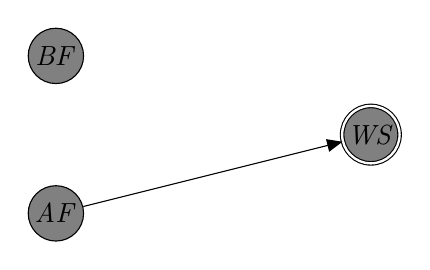
\begin{tikzpicture}
  \tikzset{neuron/.style = {shape=circle,draw,minimum size=2em,inner sep=1pt}}
    \tikzset{fireneuron/.style = {shape=circle,draw,minimum size=2em,inner sep=1pt, fill=gray}}
        \tikzset{sneuron/.style = {shape=circle,draw,minimum size=2em,inner sep=1pt, double, double distance=0.3mm}}
    \tikzset{sfireneuron/.style = {shape=circle,draw,minimum size=2em,inner sep=1pt, fill=gray,double, double distance=0.3mm}}
  \tikzset{edge/.style = {->,> = latex'}}
  \tikzset{%
  tipA/.tip={Triangle[angle=45:6pt]},
}

	\node[fireneuron] (AF) at (0,0) {$\mathit{AF}$};
	\node[fireneuron] (BF) at (0,2) {$\mathit{BF}$};
	
	\node[sfireneuron] (WS) at (4,1) {$\mathit{WS}$};
	
    \foreach \from/\to in {}
    \path[-*](\from) edge node [above]{} (\to);
    
    \foreach \from/\to in {AF/WS}
    \path[-tipA](\from) edge node [above]{} (\to);

\end{tikzpicture}
\end{center}


\end{example}

Intuitively one would declare $AF$ to be the cause of $WS$. This can be established by using basic counterfactual reasoning. That is, if Alice would not have fired the bullet, the window would not have shattered. 
Moreover, as $BF$ is not considered to be a cause as the value of $BF$ is immaterial in determining the value of $WS$.
While this example is fairly trivial, even small modifications suffice to create disagreement among definitions and intuitions alike (see Example \ref{ex:over-1}).


The following example, originally given in the context of forest fires, is frequently used by Halpern, e.g.\ \parencite{halpern2011actual,halpern2015graded}, as a benign introductory example.
Especially in the context of his definitions for token causality (\hpo, \hpu and \hpm), the impact of minimality conditions within can be observed.

\begin{example}
\label{ex:basic-2}
Alice ($\mathit{AF}$) and Bob ($\mathit{BF}$) each fire a bullet at a window, simultaneously striking the window. The window only shatters ($\mathit{WS}$), if it is hit by two bullets. What caused the window to shatter? \\

%\emph{Neuron Diagram:} 
In the neuron diagram below the only thing of note is the use of a stubborn neuron that fires only if more than two stimuli are received.
\begin{center}
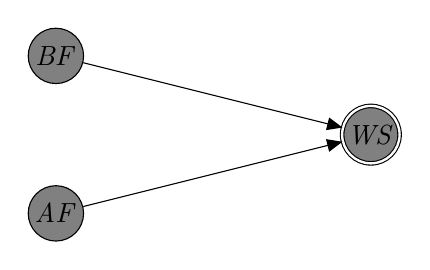
\begin{tikzpicture}
  \tikzset{neuron/.style = {shape=circle,draw,minimum size=2em,inner sep=1pt}}
    \tikzset{fireneuron/.style = {shape=circle,draw,minimum size=2em,inner sep=1pt, fill=gray}}
        \tikzset{sneuron/.style = {shape=circle,draw,minimum size=2em,inner sep=1pt, double, double distance=0.3mm}}
    \tikzset{sfireneuron/.style = {shape=circle,draw,minimum size=2em,inner sep=1pt, fill=gray,double, double distance=0.3mm}}
  \tikzset{edge/.style = {->,> = latex'}}
  \tikzset{%
  tipA/.tip={Triangle[angle=45:6pt]},
}

	\node[fireneuron] (AF) at (0,0) {$\mathit{AF}$};
	\node[fireneuron] (BF) at (0,2) {$\mathit{BF}$};
	
	\node[sfireneuron] (WS) at (4,1) {$\mathit{WS}$};
	
    \foreach \from/\to in {}
    \path[-*](\from) edge node [above]{} (\to);
    
    \foreach \from/\to in {AF/WS, BF/WS}
    \path[-tipA](\from) edge node [above]{} (\to);

\end{tikzpicture}
\end{center}
\end{example}

%
%\emph{Causal Model:} 
%\begin{equation*}
%\begin{split}
%&\{AF \mapsto 1, BF \mapsto 1\} \\
%&WS := AF \land BF
%\end{split}
%\end{equation*}
%Of note here is that logic based formulation of the equation for $WS$ was chosen. 
%Alternatively, it would have been possible to express this equation as $WS := \min(AF, BF)$. \\
%



%A variant of this Example, investigating the causes of a forest fire, is commonly used by Halpern, e.g.\ \parencite{halpern2011actual,halpern2015graded,halpern2016actual}, to introduce the concept of structural equations. 
Already in such a small example, it becomes difficult to asses what a token cause should be. 
The first possibility would be to consider $AS$, $BS$ and the conjunct of $AS$ and $BS$ as causes for $WS$.
The second possibility is the rejection of the conjunct as cause for $WS$. That is, only $AS$ and $BS$ are declared as such.
The third possibility contrasts the previous one by declaring the conjunct as the sole cause of $WS$.
For example, The minimality constraint present in all of Halpern's definitions forces those definitions to reject the conjunct \parencite[p.~28]{halpern2016actual}.


%
%\emph{Causal Models}
%\begin{equation*}
%\begin{split}
%&\{AF \mapsto 1, BF \mapsto 0\} \\
%&WS := AF 
%\end{split}
%\end{equation*}
%


%Variants of this example can be found in \parencite{beckers2018principled}.

%This example demonstrates counterfactual dependence, which according to \parencite{beckers2018principled}, is widely accepted to sufficient for establishing causation. 





\subsection{Symmetric Overdetermination}
%2 /  12
Symmetric Overdetermination is one of the problems that provides some difficulties to the counterfactual approach, leading to development of fairly complicated analytical tools.
Intuitively, an outcome can be considered overdetermined, if there are multiple processes,  which produce said outcome, terminating at the same time. 
The subsequent example is a variant of the forest fire example found in several of Halpern's publications, e.g.\  \parencite{halpern2011actual,halpern2015graded}.
Moreover, this variants of this examples are heavily used discussed, e.g.\ \parencite{glymour2010actual,halpern2011actual,baumgartner2013regularity,halpern2015graded,weslake2015partial,blanchard2017cause,wright2017ness,
bochman2018actual,beckers2018principled,denecker2018causal,batusov2018situation,denecker2019explaining,liepicna2020arguing}.

\begin{example}
\label{ex:over-1}
Alice ($AF$) and Bob ($BF$) each fire a bullet at a window, simultaneously striking the window, shattering it ($WS$). What caused the window to shatter? 

\begin{center}
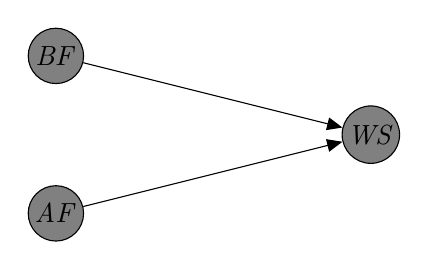
\begin{tikzpicture}
  \tikzset{neuron/.style = {shape=circle,draw,minimum size=2em,inner sep=1pt}}
    \tikzset{fireneuron/.style = {shape=circle,draw,minimum size=2em,inner sep=1pt, fill=gray}}
        \tikzset{sneuron/.style = {shape=circle,draw,minimum size=2em,inner sep=1pt, double, double distance=0.2mm}}
    \tikzset{sfireneuron/.style = {shape=circle,draw,minimum size=2em,inner sep=1pt, fill=gray,double, double distance=0.2mm}}
  \tikzset{edge/.style = {->,> = latex'}}
  \tikzset{%
  tipA/.tip={Triangle[angle=45:6pt]},
}

	\node[fireneuron] (AF) at (0,0) {$\mathit{AF}$};
	\node[fireneuron] (BF) at (0,2) {$\mathit{BF}$};
	
	\node[fireneuron] (WS) at (4,1) {$\mathit{WS}$};
	
    \foreach \from/\to in {}
    \path[-*](\from) edge node [above]{} (\to);
    
    \foreach \from/\to in {AF/WS, BF/WS}
    \path[-tipA](\from) edge node [above]{} (\to);

\end{tikzpicture}
\end{center}
\end{example}

According to \cite{hiddleston2005causal} the correct solution for Example \ref{ex:over-1} for this answer seems to be subject of contention. That is, it is unclear whether 
$AF$ or $BF$ individually should be considered a cause or whether the conjunct of $AF$ and $BF$ are the sole cause of $WS$.

By expanding Example \ref{ex:over-1} slightly, one obtains Example \ref{ex:over-2}. Variants of this example can be found in \parencite{glymour2010actual,chockler2015causal}.

\begin{example}
\label{ex:over-2}
Alice ($AF$), Bob ($BF$), Carol ($CF$), Dave ($DF$) and Eve ($EF$) all fire at a window. The window shatters after three hits ($WS$). What is the cause of the window shattering?
%
%\emph{Causal Models:}
%\begin{equation*}
%\begin{split}
%&\{V_i \mapsto 1 \mid 1 \leq i \leq 11\} \\
%&AW := 5 > \sum_{i=1}^{11} V_i
%\end{split}
%\end{equation*}
%If voter $i$ votes for Alice then $V_i=1$ otherwise $V_i=1$.

\begin{center}
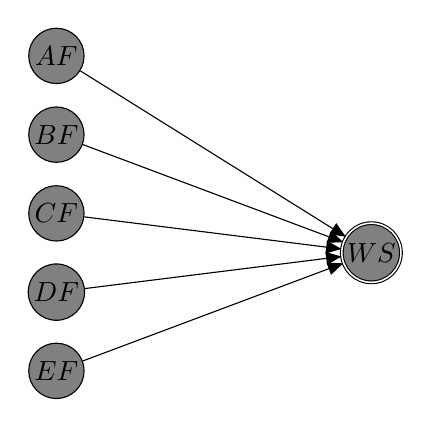
\begin{tikzpicture}
  \tikzset{neuron/.style = {shape=circle,draw,minimum size=2em,inner sep=1pt}}
    \tikzset{fireneuron/.style = {shape=circle,draw,minimum size=2em,inner sep=1pt, fill=gray}}
        \tikzset{sneuron/.style = {shape=circle,draw,minimum size=2em,inner sep=1pt, double, double distance=0.2mm}}
    \tikzset{sfireneuron/.style = {shape=circle,draw,minimum size=2em,inner sep=1pt, fill=gray,double, double distance=0.2mm}}
  \tikzset{edge/.style = {->,> = latex'}}
  \tikzset{%
  tipA/.tip={Triangle[angle=45:6pt]},
}

	\node[fireneuron] (V5) at (0,1) { $EF$};
	\node[fireneuron] (V4) at (0,2) { $DF$};
	\node[fireneuron] (V3) at (0,3) { $CF$};
	\node[fireneuron] (V2) at (0,4) { $BF$};
	\node[fireneuron] (V1) at (0,5) { $AF$};

	\node[sfireneuron] (W) at (4,2.5) {$WS$};
	
    \foreach \from/\to in {}
    \path[-*](\from) edge node [above]{} (\to);
    
    \foreach \from/\to in {V1/W,V2/W,V3/W,V4/W,V5/W}
    \path[-tipA](\from) edge node [above]{} (\to);

\end{tikzpicture}
\end{center}
\end{example}


Given the story presented in Example \ref{ex:over-1}, most accounts, i.e.\ \hpu, \ptc, \bvcm, \bci and \pcps  conclude that $AF$ and $BF$ individually are considered to be the cause of $WS$ \parencite{beckers2018principled,bochman2018actual,denecker2018causal,weslake2015partial,halpern2016actual}.
However, notes are to be taken. \hpu considers $AF$ and $BF$ as the sole cause of $WS$. 
By contrast, \hpm only considers the conjunct $AF \land BF$ as the cause of $WS$. This somewhat counter-intuitive inference is justified, by arguing that $AF$ and $BF$ individually should be considered as parts of causes rather than a cause. Alternatively, he proposes that it would be best to view $AF \lor BF$ as the cause, which would hold in \hpu and \hpm \parencite[p.~29]{halpern2016actual}.
Mirroring the intuition given for \hpm's result, \parencite{beckers2018principled} argue that while $WS$ is not dependent on either $AF$ and $BF$, both contribute to $WS$ and thus both should be considered a contributing cause. 
Their account, i.e.\ \pcps differentiates between counterfactually irrelevant and strongly counterfactually irrelevant. They wager that strongly counterfactually irrelevant variables should not be considered causes, while counterfactually irrelevant could still be considered causes. Since they classify $AF$ and $BF$ only counterfactually irrelevant 




%\newcommand{\hpu}{\texttt{HP-05}}
%\newcommand{\ptc}{\texttt{PTC}}
%\newcommand{\hpm}{\texttt{HP-15 }}
%\newcommand{\bvcm}{\texttt{BV-CM}}
%\newcommand{\bci}{\texttt{BCI}}
%\newcommand{\pcps}{\texttt{PCPS}}
%\newcommand{\sccf}{\texttt{SC-CF}}









%Using causal models one can formalise the example as 
%\begin{equation*}
%\begin{split}
%\{AF \mapsto 1 , BF \mapsto 1\} \\
%WS := AF \lor BF
%\end{split}
%\end{equation*}
%Of note here is that logic based formulation of the equation for $WS$ was chosen. 
%Alternatively, it would have been possible to express this equation as $WS := \max(AF, BF)$. \\

%For example, HP-01 and HP-05 side with declaring $AF$ and $BF$ (, but not $AF \land BF$) the cause of $WS$. Alternatively, HP-15 only considers the conjunct $AF \land BF$ to be a cause of $WS$.

%The evaluation of the respective definitions are taken from \parencite{halpern2016actual}.





%
%As for Example \ref{ex:4}, an extension of Example \ref{ex:2}, one has to deal with overdetermination. Hence, while receiving $11$ votes, $6$ votes would have been sufficient for Alice's victory. 
%Being an extension of Example \ref{ex:2}, the definitions proposed by Halpern behave similarly. That is, both HP-01 and HP-05 declare each of the $11$ voters to be a cause of Alice's victory, while HP-15 proposes that each subset containing $6$ voters should be considered a cause.
%The evaluation of the respective definitions are taken from \parencite{halpern2016actual}.



\subsection{Switching}
% The right hand of the ambidextrous perfect marksman is bitten by a dog; he pulls the trigger with his left hand and hits the bullseye. What caused the marks- man to pull the trigger with his left hand? What caused the bullseye to be hit?
%
%Consider cases of “switching”, which have been much discussed in the philosophical literature. A train is heading toward the station. An engineer throws a switch, directing the train down the left track, rather than the right track. The tracks re-converge before the station, and the train arrives as scheduled. Was throwing the switch a cause of the train’s arrival?
%
%A two-state switch is wired to two lamps. If the switch is in one state (S = 0), only lamp one is activated (L1 = 1), and if it is in the other state (S = 1) only lamp two is activated (L2 = 1). In fact, lamp two is activated and the room is illuminated (I = 1).
%
%Example 9 (Purple flame). Jones puts potassium salts (P) into a hot fire (F). Because potassium compounds produce a purple flame when heated, the flame changes to a purple colour (PF), though everything else remains the same. Both flames ignite some flammable material (I).
%
%Now take an alternative story: the crime syndicate hires both Assassin and Backup, with a similar task: to pickup a poison at (the same) hidden place and poison victim. Assas- sin is ordered to go to the hiding place on Monday, Backup on Tuesday. The syndicate puts one potion of poison in the location on Sunday.
%Before moving on towards the phenomena of preemption, a related issue should be discussed. Namely that of switching. 
Examples discussing switching are usually build as follows. There is a variable representing some form of action, e.g.\ the flicking of a switch, irrespective of the variable's value
a causal process is triggered. Each of those processes produce the same outcome. Hence, the original action was immaterial in the occurrence of said outcome.
For the binary case, this effect can be observed in the following example, variants of which can be found in \parencite{glymour2010actual,halpern2011actual,baumgartner2013regularity,weslake2015partial,bochman2018actual,beckers2018principled,denecker2018causal,batusov2018situation,denecker2019explaining}. 

\begin{example}
\label{ex:switch-1}
Alice flicks a switch ($AF$). The train travels on track $A$ ($TA$), otherwise the train would have travelled on track $B$ ($TB$). 
In both cases the train arrives at its destination ($TD$). Was $AF$ the cause of $TD$?
\end{example}

%
%\emph{Causal Model}
%
%\begin{equation*}
%\begin{split}
%&\{AF \mapsto 1\}\\
%&TA:=AF, \quad TB:=\neg AF, \quad TD:= TB \lor TB
%\end{split}
%\end{equation*}

\begin{center}
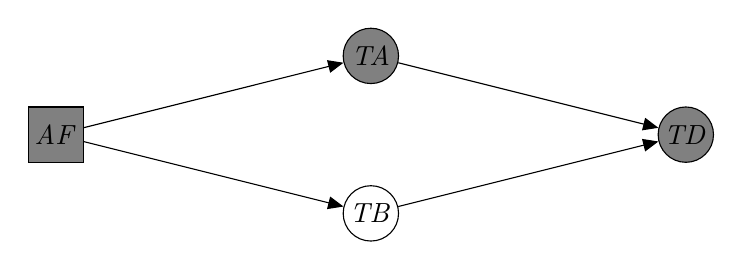
\begin{tikzpicture}
  \tikzset{neuron/.style = {shape=circle,draw,minimum size=2em,inner sep=1pt}}
    \tikzset{fireneuron/.style = {shape=circle,draw,minimum size=2em,inner sep=1pt, fill=gray}}
      \tikzset{switch/.style = {shape=rectangle,draw,minimum size=2em,inner sep=1pt}}
    \tikzset{fireswitch/.style = {shape=rectangle,draw,minimum size=2em,inner sep=1pt, fill=gray}}
        \tikzset{sneuron/.style = {shape=circle,draw,minimum size=2em,inner sep=1pt, double, double distance=0.2mm}}
    \tikzset{sfireneuron/.style = {shape=circle,draw,minimum size=2em,inner sep=1pt, fill=gray,double, double distance=0.2mm}}
  \tikzset{edge/.style = {->,> = latex'}}
  \tikzset{%
  tipA/.tip={Triangle[angle=45:6pt]},
}

	\node[fireswitch] (AF) at (0,1) {$\mathit{AF}$};
	\node[fireneuron] (TA) at (4,2) {$\mathit{TA}$};
	\node[neuron] (TB) at (4,0) {$\mathit{TB}$};
	
	\node[fireneuron] (TD) at (8,1) {$\mathit{TD}$};
	
    \foreach \from/\to in {}
    \path[-*](\from) edge node [above]{} (\to);
    
    \foreach \from/\to in {AF/TA, AF/TB, TB/TD, TA/TD}
    \path[-tipA](\from) edge node [above]{} (\to);

\end{tikzpicture}
\end{center}

With the flicking of the switch being immaterial, it proclaimed in \parencite{beckers2018principled} that most people would reject calling $AF$ a cause of $TD$. 
Although this view is not uncontroversial, especially as embracing it requires one to accept that causation is not transitive. 
That is, it is clear that $AF$ is the cause of $TA$, yet it is not the cause of $TD$. More about this discussion can be found in XXXXX.
Moreover, the formalisation presented in Example \ref{ex:switch-1} is also subject of contention. In particular, in the given model $AT$ and $BT$ being logically independent. However, this would allow for the possibility 
of the train being on two tracks at the same time. One possible method of mitigating this inaccuracy is to replace the variables $AT$ and $BT$ with the exogenous variables $BA$ and $BB$.
Those variables indicate whether a track is blocked or not. For example, if $BA$ and $AF$, then $TD$ would not hold, while in the case of $\neg AF$ the train would still arrive \parencite{halpern2011actual}.

In the context of switching there are examples were the intuition is less clear. That is, consider Example \ref{ex:switch-2}, which is discussed in \parencite{weslake2015partial,bochman2018actual}

\begin{example}
\label{ex:switch-2}
Alice pushes Bob. Therefore, Bob is hit by a truck. Bob is dies.
Otherwise, Bob would have been hit by a bus, which would have killed him as well.
\end{example}

In Example \ref{ex:switch-2} one is clearly faced with an instance of switching. However, \parencite{mcdermott1995redundant} claims that intuition would dictate that Alice did in fact kill Bob.
\parencite{weslake2015partial} argues that this intuition is a product of hidden assumption, namely that the assumption (or hope) there would be another option, like ``Push Bob to safety'' would be available.
He therefore, claims that Example \ref{ex:switch-2} is underspecified.
To retain the intuition regarding switching he suggests that one should declaring the available option as exhaustive and only omit those options that result in the same outcome.
As otherwise, i.e.\ the case where one mentions that the modelled options are not exhaustive and omits some options with a different outcome, one should consider the switch, in this case Alice's action,  a cause.


Given the story of Example \ref{ex:switch-1}, the definitions \hpu and \hpm claim $AF$ to be the cause of $TD$.
While the definitions \ptc,  \bvcm,  \bci, \scacc, \sccf and \pcps, do not \parencite{beckers2018principled,bochman2018actual,denecker2018causal,weslake2015partial,halpern2015modification,batusov2018situation}.
To bridge the gap between  \hpu, \hpm and the rest of the definitions, \parencite{halpern2015modification} resolves this issue by appealing to normality.
Furthermore, It must be noted that \hpm does not declare $AF$ a cause of $TD$, if one chooses the formalisation using $BA$ and $BB$ instead.
By contrast, \hpu still declares $AF$ to be a cause \parencite{halpern2015modification}. 


%\subsection{Push}

%[Push]
%I push(P=1)Jonesinfrontofatruck(T =1),whichhits(H=1)andkills him(D = 1);ifIhadnotdoneso(P = 0),abus(B = 1)wouldhavehit (H = 1) and killed him.
%
%Version (A): re is no other action available.
%Version (B): I can push (P = 2) Jones to safety (H = 0).


%While hidden in Example \ref{ex:switch-1}, the case of switching stirs one directly into meta-physical discussion about the nature of events. 
%Meaning if the occurrence of an event is delayed, is it still the same event. As discussed in Example \ref{ex:switch-2} taken from \parencite{halpern2011actual}, neglecting such a distinction during the modelling process may result in undesirable and unintuitive results.
%
%
%
%\begin{example}
%Alice plans to go camping in June ($AC$). If there is a forest fire in May ($FF_m$), Alice will not go camping.
%If Alice goes camping, she will cause a forest fire ($FF_j$). Al
%\end{example}
%
%%
%%In \parencite{halpern2011actual}, the following formalisation is advised.
%%\emph{Causal Model}
%%
%%\begin{equation*}
%%\begin{split}
%%& AC := \neg FF_m, \quad FF_j := AC \land \neg FF_m
%%\end{split}
%%\end{equation*}
%
%\emph{Neuron Diagram XXX}
%\begin{center}
%\begin{tikzpicture}
%  \tikzset{neuron/.style = {shape=circle,draw,minimum size=2em,inner sep=1pt}}
%    \tikzset{fireneuron/.style = {shape=circle,draw,minimum size=2em,inner sep=1pt, fill=gray}}
%      \tikzset{switch/.style = {shape=rectangle,draw,minimum size=2em,inner sep=1pt}}
%    \tikzset{fireswitch/.style = {shape=rectangle,draw,minimum size=2em,inner sep=1pt, fill=gray}}
%        \tikzset{sneuron/.style = {shape=circle,draw,minimum size=2em,inner sep=1pt, double, double distance=0.2mm}}
%    \tikzset{sfireneuron/.style = {shape=circle,draw,minimum size=2em,inner sep=1pt, fill=gray,double, double distance=0.2mm}}
%  \tikzset{edge/.style = {->,> = latex'}}
%  \tikzset{%
%  tipA/.tip={Triangle[angle=45:6pt]},
%}
%
%
%	\node[fireswitch] (AC) at (0,1) {$\mathit{AF}$};
%	\node[fireneuron] (TA) at (4,2) {$\mathit{TA}$};
%	\node[neuron] (TB) at (4,0) {$\mathit{TB}$};
%	
%	\node[fireneuron] (TD) at (8,1) {$\mathit{TD}$};
%	
%    \foreach \from/\to in {}
%    \path[-*](\from) edge node [above]{} (\to);
%    
%    \foreach \from/\to in {AF/TA, AF/TB, TB/TD, TA/TD}
%    \path[-tipA](\from) edge node [above]{} (\to);
%
%\end{tikzpicture}
%\end{center}
%
%
%If one would not have explicitly distinguished between the forest fire in May and the forest fire in June by using separate variables, the model would contain circularities and would allow for counter-intuitive inferences, e.g.\ creating a forest fire in June causes Alice to go camping \parencite{halpern2011actual}.  
%
%
%\begin{example}(Switch \cite{Weslake2015partialtheory})
%A two-state switch is wired to two lamps. If the switch is in one state ($S:=1$), only lamp one is activated ($L_1:= \neg S$), and if it is in the other state ($L_2:= S$) only lamp two is activated ($L_2=1$). In fact, lamp two is activated and the room is illuminated ($I=1$).
%\begin{equation*}
%\begin{split}
%&S:=1\\
%& L_1:= \neg S, \quad L_2:=S, \quad I:= L_1 \lor L_2
%\end{split}
%\end{equation*}
%\begin{center}
%\begin{tikzpicture}
%  \tikzset{vertex/.style = {shape=circle,draw,minimum size=2em,inner sep=1pt}}
%  \tikzset{edge/.style = {->,- = latex'}}
%
%  
%  
%	\node[vertex] (S) at (0,1.5) {$S$};
%	\node[vertex] (L1) at (4,0) {$L_1$};
%		\node[vertex] (L2) at (4,3) {$L_2$};
%	\node[vertex] (I) at (8,1.5) {$I$};
%	
%       \foreach \from/\to in {S/L1, S/L2, L1/I, L2/I}
%    \path[->](\from) edge node [above]{} (\to);
%\end{tikzpicture}
%\end{center}
%\end{example}


\subsection{Late Preemption}

%A and B each fire a bullet at a target. A’s bullet travels faster, knocking out the bullseye (D), which B’s bullet would have knocked out a moment later (D’) otherwise. What caused the event D = 1, of the bullseye’s removal?
%
%
%Suzy and Billy both pick up rocks and throw them at a bottle. Suzy’s rock gets there first, shattering the bottle. Since both throws are perfectly accurate, Billy’s would have shattered the bottle had Suzy not thrown.
%
%
%Example 5 (Simplified Bottle). Suzy (ST) and Billy (BT) both throw rocks at a bottle, but Suzy’s rock arrives first and shatters the bottle (BS). Both throws are accurate: Billy’s would have shattered the bottle if Suzy’s had not.
%
%The second scenario is similar, except that arsenic, in addition to poisoning the vic- tim, also preempts the chemical process by which strychnine poisons the victim.
%
%
%C is a traveller in the desert, whose only source of water is a keg full of water. A adds a fatal dose of undetectable poison to the water in the keg, for which there is no antidote. C remains unaware of the poison in the water. Subsequently, before C drinks any of the poisoned water, B dumps the poisoned water out of the keg. When C attempts to drink water from the keg, she discovers that it is empty. C dies due to dehydration.
%C drinks a fatal dose of poison for which there is no antidote but which takes several hours to produce death. While C is still alive, D shoots C in the head. C dies a few min- utes later from the bullet wound, well before the time at which the death by poisoning would otherwise have occurred.
%A ship is traveling down a river to deliver goods to Metropolis by a specific date. The ship is unable to arrive by that date, since its crew must and does stop when it reaches bridge A, which had collapsed into and blocked the river. The ship would not have been able to reach Metropolis on time even if bridge A had not collapsed, due to another collapsed bridge, bridge B, of which the ship’s crew was unaware, located on the river between bridge A and Metropolis.
%
%

Late preemption, is on the surface similar to symmetric overdetermination. In fact, it is sometimes called asymmetric overdetermination \parencite{erwig2010causal}. In particular, one can refer to late preemption, 
if there are two causal processes running in parallel. Each of them would produce the same outcome. However, as one process terminates before the other does. Thereby, bringing forth the outcome and rendering the second 
process irrelevant. Hence, late preemption distinguishes itself from symmetric overdetermination, based on the fact that the two running processes are temporally not aligned \parencite{beckers2018principled}.

\begin{example}
\label{ex:late-preemption-1}
Alice ($AF$) and Bob ($BF$) each fire a bullet at a window. Alice's bullet hits the window first ($AH$). The window shatters ($WS$). Bob's bullet arrives second and does not hit the window ($BH$). What caused the window to shatter?
\begin{center}
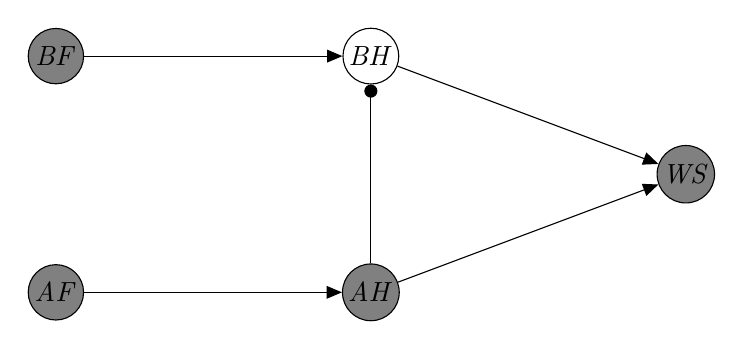
\begin{tikzpicture}
  \tikzset{neuron/.style = {shape=circle,draw,minimum size=2em,inner sep=1pt}}
    \tikzset{fireneuron/.style = {shape=circle,draw,minimum size=2em,inner sep=1pt, fill=gray}}
        \tikzset{sneuron/.style = {shape=circle,draw,minimum size=2em,inner sep=1pt, double, double distance=0.2mm}}
    \tikzset{sfireneuron/.style = {shape=circle,draw,minimum size=2em,inner sep=1pt, fill=gray,double, double distance=0.2mm}}
  \tikzset{edge/.style = {->,> = latex'}}
  \tikzset{%
  tipA/.tip={Triangle[angle=45:6pt]},
}

	\node[fireneuron] (AF) at (0,0) {$\mathit{AF}$};
	\node[fireneuron] (BF) at (0,3) {$\mathit{BF}$};
	
	\node[fireneuron] (AH) at (4,0) {$\mathit{AH}$};
	\node[neuron] (BH) at (4,3) {$\mathit{BH}$};
	
	\node[fireneuron] (WS) at (8,1.5) {$\mathit{WS}$};
	
    \foreach \from/\to in {AH/BH}
    \path[-*](\from) edge node [above]{} (\to);
    
    \foreach \from/\to in {AF/AH, BF/BH, BH/WS, AH/WS}
    \path[-tipA](\from) edge node [above]{} (\to);

\end{tikzpicture}
\end{center}
The square neuron represents a switch. That is, depending on the status of the switch either the first or the second direct successor neuron will fire.
\end{example}

%\emph{Causal Model:} 
%\begin{equation*}
%\begin{split}
%&\{AF \mapsto 1 , BF \mapsto 1\} \\
%&AH:= AF, \quad BH:= BF \land \neg AH, \quad WS := AH  \lor BH 
%\end{split}
%\end{equation*}

The intuition with this example is clear. $AF$ is the cause of $WS$. Because, Alice's bullet prevents Bob's bullet to hit the widow, by hitting it earlier.
Hence, $BF$ can not be a cause of $WS$.

%
%
%However, bringing 
%
%
%In this particular case, human intuition clearly suggests that Alice was the cause of the window's shattering. 
%This intuition is captured by HP-01, HP-05 and HP-15 all of which agree that $AF$ is the cause of $WS$.
%The evaluation of the respective definitions are taken from \parencite{halpern2016actual}. \\
The similarities to symmetric overdetermination, demonstrate serve as a good example for highlighting the importance of proper modelling.
As neglecting to model the relationship between Alice's and Bob's actions, results in a case of symmetric overdetermination. 
The model presented avoids this by adding additional variables, i.e.\ $AH$ and $BH$. That  is, there must be a variable that exhibits a different value depending the actual cause \parencite{halpern2011actual}.
An alternative approach suggested in \parencite[p.~34]{halpern2016actual} is to encode temporal information into the model by introducing time indexed variables.
Irrespectively of the additional difficulty of constructing a suitable model, the alternative approach is arguably the more intuitive one. In particular, \parencite{beckers2018principled} criticise the formalisation presented in 
Example \ref{ex:late-preemption-1} on the grounds that that $AF$ and $BF$ trigger entirely different mechanisms. Hence, constructing a model that incorporates such a relationship is conceptually wrong.
Especially, as it is obvious that Bob failed to hit the window, considering that Alice hit the window before him, i.e.\ Bob was too late. Hence, the addition of $AH$ and $BH$ simply hide the temporal aspect of the story, by implicitly encoding the order at which the bullets would hit the window, without explicitly assigning a timing to the events.
The state that the principle of ``causes come before - or at most simultaneous with - effects'' is accepted across the board. Therefore, they extend causal models with a timing function.

Abstracting away from the story \parencite{baumgartner2013regularity} provides a different late preemption example using solely neuron diagrams. 

\begin{center}
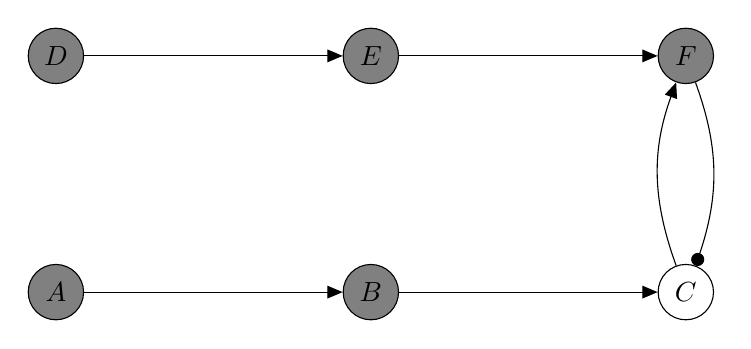
\begin{tikzpicture}
  \tikzset{neuron/.style = {shape=circle,draw,minimum size=2em,inner sep=1pt}}
    \tikzset{fireneuron/.style = {shape=circle,draw,minimum size=2em,inner sep=1pt, fill=gray}}
        \tikzset{sneuron/.style = {shape=circle,draw,minimum size=2em,inner sep=1pt, double, double distance=0.2mm}}
    \tikzset{sfireneuron/.style = {shape=circle,draw,minimum size=2em,inner sep=1pt, fill=gray,double, double distance=0.2mm}}
  \tikzset{edge/.style = {->,> = latex'}}
  \tikzset{%
  tipA/.tip={Triangle[angle=45:6pt]},
}

	\node[fireneuron] (A) at (0,0) {$A$};
	\node[fireneuron] (B) at (4,0) {$B$};
	\node[neuron] (C) at (8,0) {$C$};
	\node[fireneuron] (D) at (0,3) {$D$};
	\node[fireneuron] (E) at (4,3) {$E$};
	\node[fireneuron] (F) at (8,3) {$F$};


	
    \foreach \from/\to in {}
    \path[-*](\from) edge node [above]{} (\to);
    
    
    \path[-*](F) edge  [bend left=20] node [above]{} (C);
    
    \foreach \from/\to in {A/B, B/C, D/E, E/F}
    \path[-tipA](\from) edge node [above]{} (\to);
    
      \path[-tipA](C) edge [bend left=20] node [above]{} (F);

\end{tikzpicture}
\end{center}

Mapping this formalisation onto the story Example \ref{ex:late-preemption-1}. $F$ would be $WS$, $E$ would be $AF$, $B$ would be $BF$ and $D$ would be $AF$ ($A$ has no counterpart).
Meaning that given this structure, it was the shattering of the window that prevented Bob from hitting the window. Clearly, a sensible formalisation of the problem.
This, arguably more intuitive, formalisation, however, requires circularity. Given the given context having such a circular dependence is innocuous. Unfortunately, a slight 
change of the exogenous variables, i.e.\ setting $AF$ to false, results in the shattering of the window, without Bob's bullet hitting it. XXX
Hence, while \parencite{baumgartner2013regularity} claims that this is a canonical representation of late preemption, it seems to differ from the common formalisation of Example \ref{ex:late-preemption-1}.


The accounts \hpu, \hpm, \ptc, \bvcm, \bci, \scacc, \sccf and \pcps satisfy the provided intuition for the story presented in Example \ref{ex:late-preemption-1}. \parencite[p.~33]{beckers2018principled,bochman2018actual,denecker2018causal,weslake2015partial,khannecessary,halpern2016actual}
\bvcm being equipped with a timing function, it can serve the provided intuition wile using a model similar to the symmetric overdetermination one \parencite{beckers2018principled}.




\subsection{Early Preemption}
%Example 6 Suzy throws a rock at a bottle. The rock hits it, and the bottle breaks. However Billy was watching Suzy, and would have thrown a rock just in case Suzy did not throw.
%
%If Trainee shoots his gun (T), the bullet will hit Victim (V). If Trainee does not shoot, Supervisor will shoot and hit Victim herself (S). In fact, Trainee shoots and hits Victim while Supervisor stands by.
%T := 1
%S := -T
%V := T ∨ S
%
%Assassin decides to poison the meal of a victim, who subsequently Dies right before dessert. However, Murderer decided to murder the victim as well, so he poisoned the dessert. If Assassin had failed to do his job, then Backup probably would have done so all the same.
%
%Billy has set the alarm for six o’clock, at which time it goes off, so that he and Suzy make it in time to school. However, Suzy had put her alarm for five past six, which would have also left ample amount of time. If Billy had failed to put his alarm, then Mother probably have done so all the same.
%
%Example 6. (Backup (Hitchcock 2007) (early preemption versus switch)) A crime syndicate hires Assassin to poison victim’s water who drinks it and dies. The syndicate had hired Backup to watch Assassin and to poison the victim in case Assassin would not poison the water. Backup did not have to intervene. This scenario is a case of early preemp- tion (of the poisoning by Backup). Three causal mechanisms can be discerned. They are represented:
%
Many authors consider early and late preemption to be the same (or at least similar), thus they resolve examples discussing early preemption in a similar fashion.
The difference between those two is, that in early preemption the outcome of the two processes occurred before the second process was in motion \parencite{beckers2018principled}.
Example \ref{ex:early-preemption-1} seems to be a canonical example for this effect, variants of it can be found in \parencite{baumgartner2013regularity,halpern2015graded,weslake2015partial,beckers2016general,blanchard2017cause,wright2017ness,
fenton2017proposed,bochman2018actual,beckers2018principled,batusov2018situation,denecker2019explaining}.


\begin{example}(Early Preemption)
\label{ex:early-preemption-1}
Alice fires a bullet at the window ($AF$). If Alice hits the window ($AH$), the window shatters ($WS$).
If Alice does not hit the window, Bob fires a bullet at the window ($BF$), hitting it ($BH$) leading to its shattering.
What caused the window to shatter?

In the neuron diagram the neuron $B$ is used to ensure that $BF$ fires per default. 
That is, it allows $BF$ to fire if $A$ does not fire, i.e.\ they together encode the behaviour of a negation.
\begin{center}
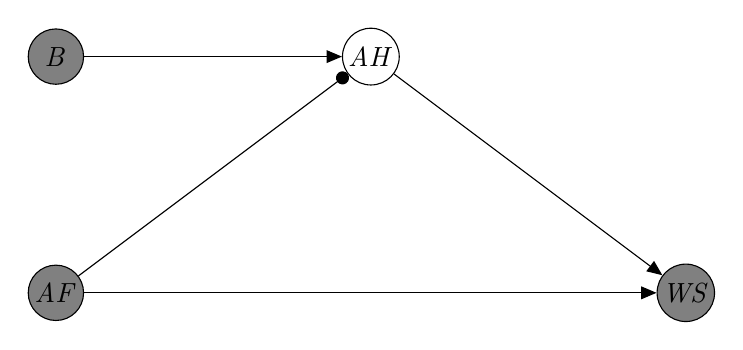
\begin{tikzpicture}
  \tikzset{neuron/.style = {shape=circle,draw,minimum size=2em,inner sep=1pt}}
    \tikzset{fireneuron/.style = {shape=circle,draw,minimum size=2em,inner sep=1pt, fill=gray}}
        \tikzset{sneuron/.style = {shape=circle,draw,minimum size=2em,inner sep=1pt, double, double distance=0.2mm}}
    \tikzset{sfireneuron/.style = {shape=circle,draw,minimum size=2em,inner sep=1pt, fill=gray,double, double distance=0.2mm}}
  \tikzset{edge/.style = {->,> = latex'}}
  \tikzset{%
  tipA/.tip={Triangle[angle=45:6pt]},
}

	\node[fireneuron] (AF) at (0,0) {$\mathit{AF}$};
	\node[fireneuron] (B) at (0,3) {$\mathit{B}$};
	
	\node[neuron] (BF) at (4,3) {$\mathit{AH}$};

	\node[fireneuron] (WS) at (8,0) {$\mathit{WS}$};
	
    \foreach \from/\to in {AF/BF}
    \path[-*](\from) edge node [above]{} (\to);
    
    \foreach \from/\to in {AF/WS, BF/WS, B/BF}
    \path[-tipA](\from) edge node [above]{} (\to);

\end{tikzpicture}
\end{center}
\end{example}

As eluded to earlier, the intuition is similar to the late preemption one. That is, $AF$ is attributed to be the cause of $WS$, while $BF$ is naturally not a cause of $WS$.
However, this straight forward analysis, is deceptive. \parencite{beckers2018principled} noticed that early preemption has a close relationship with switching.
Alice, assuming that she is certain that Bob will shoot at the window if she neglects to do so, is faced with a choice.
Either she shoots the window and it shatters or Bob will shoot at the window, shattering it in the process. Regardless, the status of the window is independent of her decision. 
In fact, Alice can only choose the causal path responsible for shattering the window, i.e.\ she can decide how and not that the window shatters.
Hence, it is a case of switching. To further strengthen the similarity \parencite{denecker2019explaining} add an additional variable to the model, representing the bullet leafing the gun. In this case let it be $AH$ representing that Alice hit the window. This produces a model that is isomorphic to Example \ref{ex:switch-1}. They claim, not uncontested, see \parencite{weslake2015partial}, that adding this variable should not influence the intuition about what is the cause of what.

Excepting that, one must explain the conflicting intuitions. Some argue for the necessity of probability or some other method of expressing uncertainty in the success of the causal process \parencite{beckers2018principled,hall2007structural}. For example, one could argue that people assume the Bob firing and hitting the window may not succeed, while the arrival of the train will always succeed. 
This view seems to be supported by the fact that if one attaches probabilities of arrival to the respective railway tracks found in Example \ref{ex:switch-1}, some causal attribution is warranted. 
For example, if on track $A$ the train has a $99\%$ chance of arrival and on track $B$ the train has a $1\%$ chance, then Alice's flicking of the switch contributed in the trains arrival.
Such an asymmetry can be observed in an example taken from \parencite{beckers2018principled}
 \begin{example}[\cite{beckers2018principled}]
\label{ex:early-preemption-3}
Suppose Alice reach out and catch a passing cricket ball. The next thing along in the ball’s direction of motion was a solid brick wall. Beyond that was a window.
\end{example}
People tend to classify this example as an instance of switch. That is, catching the ball is immaterial for the status of the window.
However, by replacing the wall with another person Bob, this intuition shifts, declaring Alice's action to be the causal for the well being of the window.
The presumption is that, this asymmetry arises due to the fact the prospect of the wall failing to stop the ball is not taken seriously \parencite{beckers2018principled,blanchard2017cause}.

\parencite{denecker2019explaining} resolve this issue by distinguishing between enabling and triggering conditions. 
The prior preempts the causal mechanism if not present, while the latter setts the mechanism in operation.
Considering the discussed cases. Alice's flicking of the switch would be merely an enabling condition for the train taking track $A$ or track $B$. By contrast, Alice's firing of the bullet is clearly a triggering condition for the bullet hitting the window.


Another example that highlight the similarities and differences between switching and early preemption is Example \ref{ex:early-preemption-3}.

 \begin{example}[\cite{weslake2015partial}]
\label{ex:early-preemption-3}
Two two-state switches are wired to an electrode. The switches are controlled by $A$ and $B$ respectively, and the electrode is attached to $C$. $A$ has the first option to flip her switch. $B$ has the second option to flip her switch. The electrode is activated and shocks $C$  if both switches are in the same position. $B$ wants to shock $C$, and so flips her switch iff $A$ does.
 \end{example}
 
 This example shares similarity with switch and early preemption, it can be found in \parencite{weslake2015partial,bochman2018actual}. 
 While structurally similar to early preemption, one could argue that the action of $A$ does not trigger the shocking of $C$ and thus it should rather be considered to be a case of switching. 
 Intuition would suggest that interpreting this example as a species of switch, would be more apt. That is, $A$ having no choice in the matter should not be considered a cause of $C$.


Furthermore, similar to late preemption, \parencite{baumgartner2013regularity} attributes early preemption a structure that is (slightly) different to the one presented in Example \ref{ex:early-preemption-1}.
However, in this case the structure actually corresponds with the model extension used by \parencite{denecker2019explaining} to further highlight the similarities to switching.
That is, $A$ is $AF$;  $C$ is $BF$; $D$ is $AH$; $R$ is $WS$; $B$ is is used as mentioned in Example \ref{ex:early-preemption-1}
\begin{center}
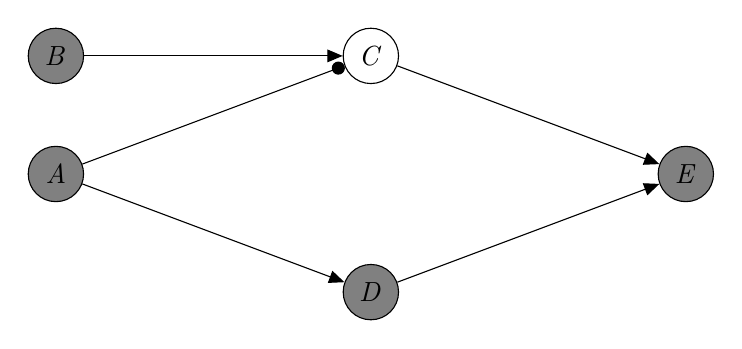
\begin{tikzpicture}
  \tikzset{neuron/.style = {shape=circle,draw,minimum size=2em,inner sep=1pt}}
    \tikzset{fireneuron/.style = {shape=circle,draw,minimum size=2em,inner sep=1pt, fill=gray}}
        \tikzset{sneuron/.style = {shape=circle,draw,minimum size=2em,inner sep=1pt, double, double distance=0.2mm}}
    \tikzset{sfireneuron/.style = {shape=circle,draw,minimum size=2em,inner sep=1pt, fill=gray,double, double distance=0.2mm}}
  \tikzset{edge/.style = {->,> = latex'}}
  \tikzset{%
  tipA/.tip={Triangle[angle=45:6pt]},
}

	\node[fireneuron] (AF) at (0,1.5) {$\mathit{A}$};
	\node[fireneuron] (B) at (0,3) {$\mathit{B}$};
	
	\node[neuron] (BF) at (4,3) {$\mathit{C}$};
	\node[fireneuron] (AH) at (4,0) {$\mathit{D}$};

	\node[fireneuron] (WS) at (8,1.5) {$\mathit{E}$};
	
    \foreach \from/\to in {AF/BF}
    \path[-*](\from) edge node [above]{} (\to);
    
    \foreach \from/\to in {AF/AH, AH/WS, BF/WS, B/BF}
    \path[-tipA](\from) edge node [above]{} (\to);

\end{tikzpicture}
\end{center}

By comparing the neuron diagrams of Example \ref{ex:late-preemption-1} and Example \ref{ex:early-preemption-1} it is hard to ignore their striking similarity.
This would explain the fact that they are sometimes treated alike. So what is exactly the difference between those two phenomena?
When observing the neuron diagrams provided in \parencite{baumgartner2013regularity} the distinction can be characterised as follows.
One speaks of early preemption, if the backup process, here $BF$, is made redundant before the effect occurs. Whereas, in late preemption the backup process is 
interrupted by the effect itself. 
An alternative distinction, claims that the characteristic feature of early preemption is that the process in question is actually interrupted by another process, while in late preemption the 
process is never interrupted, it simple never has the opportunity to terminate \parencite{baumgartner2013regularity}.


%,
The intuition presented through the story in Example \ref{ex:early-preemption-1} is satisfied by \hpu, \hpm, \ptc, \bci, \scacc, \sccf and \pcps \parencite{bochman2018actual,denecker2018causal,weslake2015partial,batusov2018situation}.
This result is deliberately not shared by \bvcm.
As eluded to earlier, \parencite{beckers2018principled} understands the usual formalisation of this example as switch. Hence, \bvcm does not declare $AF$ to be the cause of $WS$.
However, by properly extending the model with variables representing the accuracy of either Alice or Bob, $AF$ becomes a cause.
In the case of \bci, Alice is not only the cause of the window's shattering when she fires her bullet, but also when she does not. This result is particularly interesting in the context of the discussion in \parencite{beckers2018principled}.
That is, in \parencite{bochman2018actual} $AF$ could be considered as a variable that switches between two processes with the same outcome. However, rather than intuition declaring the switch to be irrelevant for the occurrence of the outcome, it is always considered a cause of the outcome.





%
%
%\emph{Causal Model:} 
%\begin{equation*}
%\begin{split}
%&\{AF \mapsto 1 , BF \mapsto 1\} \\
%&AH:= AF, \quad BH:= BF \land \neg AH, \quad WS := AH  \lor BH 
%\end{split}
%\end{equation*}

%\emph{Neuron Diagram:} 

%
%\begin{example}(Shock \cite{Weslake2015partialtheory})
%Two two-state switches are wired to an electrode. The switches are controlled by $A$ and $B$ respectively, and the electrode is attached to $C$. $A$ has the first option to flip her switch ($A=1$). $B$ has the second option to flip her switch ($B=1$). The electrode is activated and shocks $C$ ($C=1$) iff both switches are in the same position. $B$ wants to shock $C$, and so flips her switch iff $A$ does.
%\begin{equation*}
%\begin{split}
%&A:=1\\
%& B:=A, \quad C:=(A=B)
%\end{split}
%\end{equation*}
%\begin{center}
%\begin{tikzpicture}
%  \tikzset{vertex/.style = {shape=circle,draw,minimum size=2em,inner sep=1pt}}
%  \tikzset{edge/.style = {->,- = latex'}}
%
%  
%  
%	\node[vertex] (A) at (0,0) {$A$};
%	\node[vertex] (B) at (2,1.5) {$B$};
%	\node[vertex] (C) at (4,0) {$C$};
%	
%       \foreach \from/\to in {A/B, A/C, C/B}
%    \path[->](\from) edge node [above]{} (\to);
%\end{tikzpicture}
%\end{center}
%\end{example}


\subsection{Double Preemption}
%
% A, a perfect marksman, is about to fire at the bullseye; B is about to jostle A to prevent A from hitting the bullseye; C shoves B out of the way. A fires and hits the bullseye (D). What caused the bullseye to be hit?


One speaks of double preemption if there is an process instigated to interrupt some process is prevented by yet another process. Hence, the potential preempter is preempted.
Put differently, the binary variable $A$ would not hold if the binary variable $B$ holds. However, $B$ does not hold because of $C$ \parencite{denecker2019explaining}. 
Variants of Example \ref{ex:double-preemption-1} can be found in \parencite{glymour2010actual,beckers2018principled,denecker2018causal,denecker2019explaining}.

\begin{example}
\label{ex:double-preemption-1}
Alice intends to fire a bullet at a window ($A$). 
Bob is intends to prevent Alice from hitting the window ($B$).
Bob tries to stop Alice ($BSA$).
Bob is stopped by Carol ($CSB$). 
Alice fires a bullet ($AF$), hits the window ($AH$) and shatters it ($WS$). 
The window shatters ($WS$). 
What caused the window to shatter?
\begin{center}
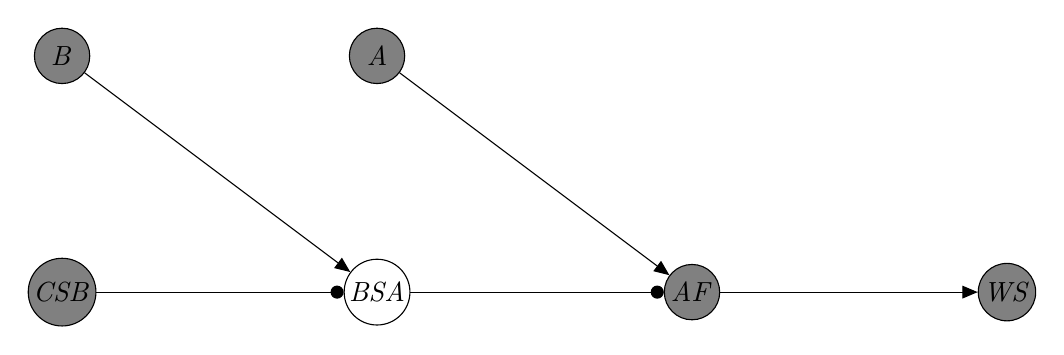
\begin{tikzpicture}
  \tikzset{neuron/.style = {shape=circle,draw,minimum size=2em,inner sep=1pt}}
    \tikzset{fireneuron/.style = {shape=circle,draw,minimum size=2em,inner sep=1pt, fill=gray}}
        \tikzset{sneuron/.style = {shape=circle,draw,minimum size=2em,inner sep=1pt, double, double distance=0.2mm}}
    \tikzset{sfireneuron/.style = {shape=circle,draw,minimum size=2em,inner sep=1pt, fill=gray,double, double distance=0.2mm}}
  \tikzset{edge/.style = {->,> = latex'}}
  \tikzset{%
  tipA/.tip={Triangle[angle=45:6pt]},
}

	\node[fireneuron] (B) at (0,3) {$\mathit{B}$};
	\node[fireneuron] (A) at (4,3) {$\mathit{A}$};
	
	\node[fireneuron] (CSP) at (0,0) {$\mathit{CSB}$};
	\node[neuron] (BSA) at (4,0) {$\mathit{BSA}$};
	\node[fireneuron] (AF) at (8,0) {$\mathit{AF}$};
	\node[fireneuron] (WS) at (12,0) {$\mathit{WS}$};
	
	
	
    \foreach \from/\to in {CSP/BSA, BSA/AF}
    \path[-*](\from) edge node [above]{} (\to);
    
    \foreach \from/\to in {A/AF, AF/WS, B/BSA}
    \path[-tipA](\from) edge node [above]{} (\to);

\end{tikzpicture}
\end{center}
The inclusion of $A$ ensures that Alice fires and hits the window by default. That is, one could remove $A$, however, this would require the specification of a default value for $AF$.
As otherwise, regardless of the specified context $AF$, being an endogenous variable, would never fire. 
The same holds for $B$.
\end{example}

According to \parencite[p.~35]{halpern2016actual}, the intuition for this example is to attribute not only $AF$, but also $CSB$ with being the causes of $WS$. 
This intuition is satisfied by all of its definitions, thus in particular \hpu and \hpm satisfy it. By contrast, \pcps does not deem $CSB$ to be the cause of $WS$. 
However, they argue that their definition can easily adapted into a sate of compliance with Halpern's proposed intuition \parencite[p.~36]{denecker2019explaining,halpern2016actual}. 



Moreover, an issue arises in the case were Bob never intends to stop Alice, i.e.\ where $B$ never fires. 
Here intuition would dictate that clearly $CSB$ can not be a cause of $WS$. This slight change of context produces counterintuitive inferences in some formalisms.
Halpern suggest that this issue is the result of a to simplistic model. That is, Carol can only stop Bob if Bob actually tries to stop Alice, a causal dependence clearly not present within the model of Example \ref{ex:double-preemption-1} 
\parencite[p.~36]{halpern2016actual}. 


\begin{center}
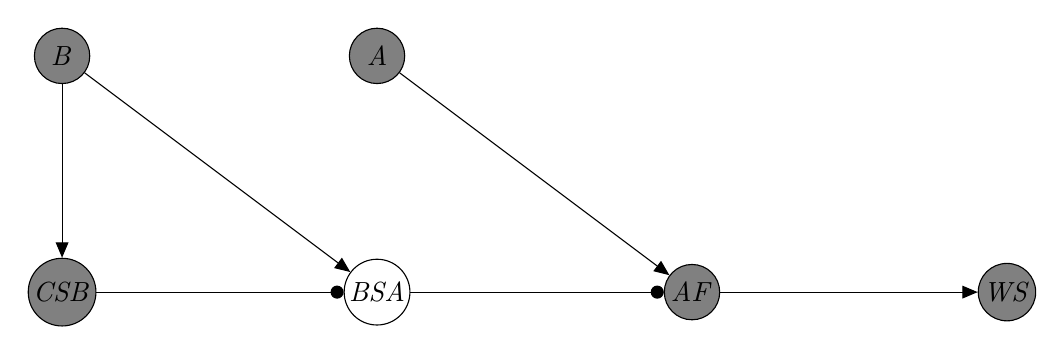
\begin{tikzpicture}
  \tikzset{neuron/.style = {shape=circle,draw,minimum size=2em,inner sep=1pt}}
    \tikzset{fireneuron/.style = {shape=circle,draw,minimum size=2em,inner sep=1pt, fill=gray}}
        \tikzset{sneuron/.style = {shape=circle,draw,minimum size=2em,inner sep=1pt, double, double distance=0.2mm}}
    \tikzset{sfireneuron/.style = {shape=circle,draw,minimum size=2em,inner sep=1pt, fill=gray,double, double distance=0.2mm}}
  \tikzset{edge/.style = {->,> = latex'}}
  \tikzset{%
  tipA/.tip={Triangle[angle=45:6pt]},
}

	\node[fireneuron] (B) at (0,3) {$\mathit{B}$};
	\node[fireneuron] (A) at (4,3) {$\mathit{A}$};
	
	\node[fireneuron] (CSB) at (0,0) {$\mathit{CSB}$};
	\node[neuron] (BSA) at (4,0) {$\mathit{BSA}$};
	\node[fireneuron] (AF) at (8,0) {$\mathit{AF}$};
	\node[fireneuron] (WS) at (12,0) {$\mathit{WS}$};
	
	
	
    \foreach \from/\to in {CSB/BSA, BSA/AF}
    \path[-*](\from) edge node [above]{} (\to);
    
    \foreach \from/\to in {A/AF, AF/WS, B/BSA, B/CSB}
    \path[-tipA](\from) edge node [above]{} (\to);

\end{tikzpicture}
\end{center}

%
%Another rather concerning issue arises when a slightly different context is considered. Namely the one where Bob never tries to stop Alice, but where Carol still anticipates that Bob will appear and will indeed try to stop Alice.
%Hence, the formalisation remains similar but for the fact that $BSA$ can never fire,
% 
%Moreover, when pairing double preemption with symmetric overdetermination additional problems arise.
Lastly, it should be noted that it does not stop with double preemption. Meaning, one could extend the causal chain by adding a fourth party preventing Carol stopping Bob \parencite{denecker2018causal}.


\subsection{Bogus Preemption}

% Assassin is in possession of a lethal poison, but has a last-minute change of heart and refrains from putting it in Victim’s water. Bodyguard puts antidote in the water, which would have neutralized the poison had there been any. Victim drinks the water and survives. Is Bodyguard’s putting in the antidote a cause of Victim surviving? Most people would say no, but according to the preliminary HP definition, it is. For in the contingency where Assassin puts in the poison, Victim survives iff Bodyguard puts in the antidote.

In essence, bogus preemption or bogus prevention occurs when an action is taken to interrupt an inactive process.
Examples discussing bogus preemption can be found in \parencite{halpern2011actual,baumgartner2013regularity,halpern2015graded,weslake2015partial,chockler2015causal,blanchard2017cause,bochman2018actual,beckers2018principled,denecker2018causal,denecker2019explaining}.
The canonical example, called ``Careful Antidote'', revolves around a poisoned water.
\begin{example}
\label{ex:bogus-preemption-0}
Alice is in possession of a lethal poison, but has a last-minute change of heart and refrains from putting it in Carol's water ($A$ - $A$ is true if Alice does \emph{not} poison the water). Bob puts antidote in the water ($B$), which would have neutralized the poison. Carol drinks the water and survives ($C$).

\begin{center}
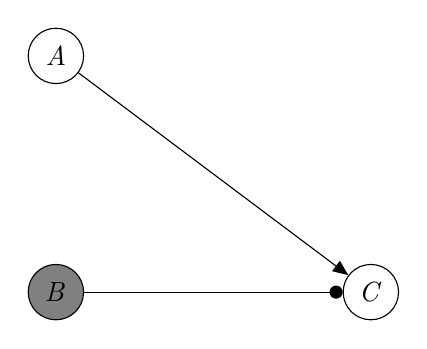
\begin{tikzpicture}
  \tikzset{neuron/.style = {shape=circle,draw,minimum size=2em,inner sep=1pt}}
    \tikzset{fireneuron/.style = {shape=circle,draw,minimum size=2em,inner sep=1pt, fill=gray}}
        \tikzset{sneuron/.style = {shape=circle,draw,minimum size=2em,inner sep=1pt, double, double distance=0.2mm}}
    \tikzset{sfireneuron/.style = {shape=circle,draw,minimum size=2em,inner sep=1pt, fill=gray,double, double distance=0.2mm}}
  \tikzset{edge/.style = {->,> = latex'}}
  \tikzset{%
  tipA/.tip={Triangle[angle=45:6pt]},
}

	\node[fireneuron] (BA) at (0,0) {$\mathit{B}$};
	\node[neuron] (AP) at (0,3) {$\mathit{A}$};

	\node[neuron] (CD) at (4,0) {$\mathit{C}$};
	
	
	
    \foreach \from/\to in {BA/CD}
    \path[-*](\from) edge node [above]{} (\to);
    
    \foreach \from/\to in {AP/CD}
    \path[-tipA](\from) edge node [above]{} (\to);

\end{tikzpicture}
\end{center}
\end{example}

The formalisation in Example \ref{ex:bogus-preemption-0} is used to demonstrate the limitation of structural equations, because while being isomorphic to the example of symmetric overdetermination the intuition underlying both 
phenomena are vastly different.
That is, Carol survives if Alice refrains from poisoning the water or if Bob adds the antidote to the water. Hence, $C$ fires if either $A$ or $B$ fires. Hence, one is confronted with symmetric overdetermination, indicating that $A$ and $B$ or their conjunct should be considered a cause of $C$. Yet, in the context of the given story, neither $A$ nor $B$ should be considered a cause.
\parencite{baumgartner2013regularity} elegantly observes that symmetric overdetermination discusses the overdetermination of occurrences, while bogus preemption is concerned with overdetermined absence.
 \parencite{halpern2011actual,weslake2015partial,halpern2015graded}.

One suggested solution to this problem is to appeal to some notion of normality. That is, in addition of formalising the causal structure, it is necessary provide the inference system with a theory of normality in order to derive suitable causes.
The idea behind this approach is that one can use the notion of normality to exclude certain unreasonable contingencies.
In this particular case, one could add a statement ``typically, people do not put poison in the water.'' to the model. Thus, the scenario where Alice actually poisons the water is less ``normal'' than the actual scenario. 
Hence, given this normality assumption, one can classify Bob's action as completely redundant. Thereby, excluding it from being a cause.
\parencite{halpern2011actual,halpern2015graded}.


Another suggestion to resolve this issue is to adapt the model used to represent the scenario. 
The aptness of the presented model is directly criticised in \parencite{blanchard2017cause}, where it is called it impoverish.
The source of such harsh words, lies in the fact the coarse nature of this formalisation ignores vital information.
To compensate this deficit \parencite{blanchard2017cause} suggest the inclusion of a variable indicating the toxicity of the water. 
In \parencite{halpern2015graded} notes, that such an extension is arguably more preferable than introducing normality.
While not explicitly criticising the approach from Example \ref{ex:bogus-preemption-0}, another frequent formalisation extends the model by a variable encoding the drinking of the water.
The prior is also found in \parencite{bochman2018actual,halpern2015graded}, the latter is discussed in \parencite{denecker2018causal,denecker2019explaining} and a combination of both can be found in 
\parencite{beckers2018principled}.
Being the most detailed, a variant of the last is presented in \ref{ex:bogus-preemption-1}. 

\begin{example}
\label{ex:bogus-preemption-1}
%Alice intents to load Carol's unsecured gun ($AL$). 
%Alice does not load Carol's unsecured gun.
%Bob secures Carol's weapon ($BS$).
%Carol pulls the trigger ($CF$).
%Pulling the trigger on a loaded an unsecured gun causes it to fire ($GF$).
%The gun does not fire.
%The window does not shatter ($WS$).
%What caused the window not to shatter?
Alice intents to put lethal poison into Carol's water ($AP$). 
However, Alice does not put lethal poison into Carol's water.
Bob puts an antidote into Carol's water ($BA$). 
The water is lethal ($L$), if the poison is added without the addition of an antidote
If Carol would consumes the lethal water she would die ($CD$). 
Carol consumes her water ($CC$). 
Carol does not die.
%What is the cause of Carol
%Alice is in possession of a lethal poison, but has a last-minute change of heart and refrains from putting it in Carol's water. Bodyguard puts antidote in the water ($B=1$), which would have neutralized the poison. Victim drinks the water and survives ($D=0$).
\begin{center}
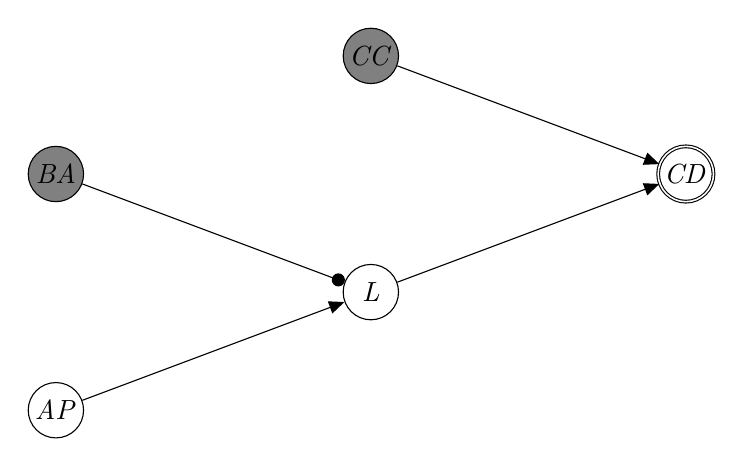
\begin{tikzpicture}
  \tikzset{neuron/.style = {shape=circle,draw,minimum size=2em,inner sep=1pt}}
    \tikzset{fireneuron/.style = {shape=circle,draw,minimum size=2em,inner sep=1pt, fill=gray}}
        \tikzset{sneuron/.style = {shape=circle,draw,minimum size=2em,inner sep=1pt, double, double distance=0.2mm}}
    \tikzset{sfireneuron/.style = {shape=circle,draw,minimum size=2em,inner sep=1pt, fill=gray,double, double distance=0.2mm}}
  \tikzset{edge/.style = {->,> = latex'}}
  \tikzset{%
  tipA/.tip={Triangle[angle=45:6pt]},
}

	\node[neuron] (AP) at (0,0) {$\mathit{AP}$};
	\node[fireneuron] (BA) at (0,3) {$\mathit{BA}$};

	\node[neuron] (L) at (4,1.5) {$\mathit{L}$};
	\node[fireneuron] (CC) at (4,4.5) {$\mathit{CC}$};
	
	\node[sneuron] (CD) at (8,3) {$\mathit{CD}$};
	
    \foreach \from/\to in {BA/L}
    \path[-*](\from) edge node [above]{} (\to);
    
    \foreach \from/\to in {AP/L,CC/CD,L/CD}
    \path[-tipA](\from) edge node [above]{} (\to);

\end{tikzpicture}
\end{center}
\end{example}

In \parencite{weslake2015partial}, they use the simplistic formalisation found in Example \ref{ex:bogus-preemption-0}. 
Being isomorphic to switch, their formalism, i.e.\ \ptc,  naturally concludes that both $AP$ and $BA$ causally influence the status of $CD$.
A formalisation obtained by extending the one found in Example \ref{ex:bogus-preemption-0} with a variable that holds when the poison is neutralised \hpu does not declare $BA$ to be a cause.
However, on the same model, both \hpu and \hpm  consider $AF$ to be a cause \parencite[p.~88]{halpern2016actual}.
In \parencite{bochman2018actual} they use use yet again a slightly different formalisation.
That is, utilising \ct they construct a theory expressing that $AP$ and not $BA$ causes $CD$; not $AP$ causes not $CD$;
$A$ and $B$ cause not $CD$. Using this, \bci concludes that only the absence of Alice poisoning the water is the cause of Carol's survival. In \parencite{beckers2018principled}, they use their timing function to differentiate between between $AP$ and $BA$. Therefore, if Alice's actions pre-date Bob's, then Alice's decision to refrain from poisoning the water is deemed to be the cause of Carol's survival by \bvcm. By contrast, if the order is reversed, the addition of the antidote would be classified as the cause. Additionally, if no timing is given this example is treated as a case of symmetric overdetermination.
According to \parencite{denecker2019explaining}, adding an antidote does interrupt the mechanism activated by poisoning the water. However, as this never occurred the, it is impossible for $BA$ to preempt an inactive mechanism. 
Hence, only the refusal of Alice to poison the water should be considered a cause of Carol's survival.
Their discussed definition, i.e.\ \pcps, reflects this reasoning.


This example provides ample insights into the problem of omission in causal inference. XXXXX




%
%\begin{example}(Careful Poisoning \cite{Weslake2015partialtheory})
%Alice is sick on Monday ($AS_m$). If the doctor treats Alice on Monday, she is recovered on Tuesday. Otherwise,
%she remains sick on Tuesday.
%Alice is sick on Tuesday ($AS_t$)
%\begin{equation*}
%\begin{split}
%&A:=1 \\
%&B:=A, \quad D:=\neg A \land B
%\end{split}
%\end{equation*}
%\begin{center}
%\begin{tikzpicture}
%  \tikzset{vertex/.style = {shape=circle,draw,minimum size=2em,inner sep=1pt}}
%  \tikzset{edge/.style = {->,- = latex'}}
%
%  
%  
%	\node[vertex] (A) at (0,0) {$A$};
%	\node[vertex] (B) at (2,1.5) {$B$};
%	\node[vertex] (D) at (4,0) {$D$};
%	
%       \foreach \from/\to in {A/B, B/D, A/D}
%    \path[->](\from) edge node [above]{} (\to);
%\end{tikzpicture}
%\end{center}
%\end{example}


\subsection{Short Circuit }

%
%A victim has two bodyguards charged with protecting him from assassination. The bodyguards conspire to make it appear as though they have foiled an attempted poisoning. They plan to put poison in victim’s drink, and also to put in an antidote that will neutralize the poison. However, they do not want to put the poison in until they are certain that the antidote has safely been put in the drink. Thus, the first bodyguard adds antidote to the drink, and the second waits until the antidote has been added before adding the poison. If the first bodyguard were interrupted, or somehow prevented from putting the antidote in, the second would not add the poison. As it happens, both the antidote and the poison are added, so the poison is neu- tralized; the victim drinks the harmless liquid and lives.

Variants of this example, often called ``Careful Poisoning'', can be found in \parencite{baumgartner2013regularity,halpern2015graded,weslake2015partial,beckers2018principled,blanchard2017cause}.

\begin{example}(Careful Poisoning)
\label{ex:short-circuit-0}
Alice puts a harmless antidote in Carol's water ($A$). Bob intended to not put poison into the water ($IB$).
Seeing that the water contains an antidote Bob, adds the poison into the water ($B$ - $B$ holds if Bob does not administer the poison). 
This poison is countered by the antidote.  
Carol drinks the water and survives ($S$).
%Bob then poisons the water ($B$ - $B$ holds if Bob does not administer the poison), using a poison that is normally lethal, but which is countered by the antidote. Bob would not have poisoned the water if Alice had not administered the antidote first. Carol drinks the water and survives ($S$).
\begin{center}
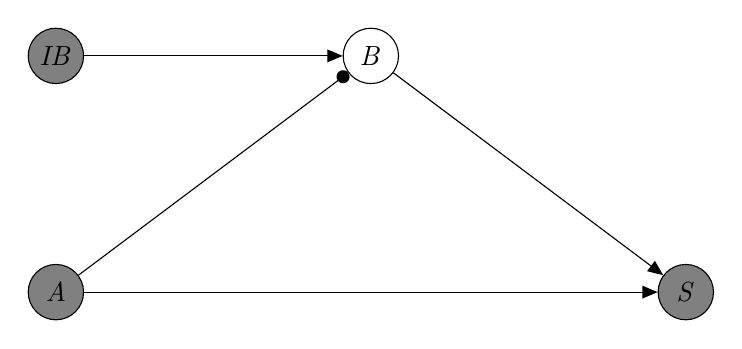
\begin{tikzpicture}
  \tikzset{neuron/.style = {shape=circle,draw,minimum size=2em,inner sep=1pt}}
    \tikzset{fireneuron/.style = {shape=circle,draw,minimum size=2em,inner sep=1pt, fill=gray}}
        \tikzset{sneuron/.style = {shape=circle,draw,minimum size=2em,inner sep=1pt, double, double distance=0.2mm}}
    \tikzset{sfireneuron/.style = {shape=circle,draw,minimum size=2em,inner sep=1pt, fill=gray,double, double distance=0.2mm}}
  \tikzset{edge/.style = {->,> = latex'}}
  \tikzset{%
  tipA/.tip={Triangle[angle=45:6pt]},
}

	\node[fireneuron] (AF) at (0,0) {$\mathit{A}$};
	\node[fireneuron] (B) at (0,3) {$\mathit{IB}$};
	
	\node[neuron] (BF) at (4,3) {$\mathit{B}$};

	\node[fireneuron] (WS) at (8,0) {$\mathit{S}$};
	
    \foreach \from/\to in {AF/BF}
    \path[-*](\from) edge node [above]{} (\to);
    
    \foreach \from/\to in {AF/WS, BF/WS, B/BF}
    \path[-tipA](\from) edge node [above]{} (\to);

\end{tikzpicture}
\end{center}
$I$ was added to encode that per default Bob does not intend to poison the water. This is necessary due to the fact that neuron diagrams (in the common use) do not have an edge reserved for a negated relation.
\end{example}


Similarly, to bogus preemption this formalisation of the presented story is isomorphic to the canonical early preemption case presented in Example \ref{ex:early-preemption-1}.
This would suggest that adding the antidote to the water caused the survival of Carol. While not entirely uncontested, intuition would dictate that neither $A$ nor $B$ should be considered a cause of $S$ \parencite{beckers2018principled}.


This example is the second one, to be referenced when talking about the limitations of structural equations and the necessity of extending causal models with some sense of normality ranking.
Again this approach is criticised by \parencite{blanchard2017cause}, citing the inaptitude of the model as source of the perceived similarities.
Precisely as before, the argue that adding a variable tracking the lethality of the water is sufficient to resolve the issue of diverging intuitions on equivalent structures. 
%
%\begin{center}
%\begin{tikzpicture}
%  \tikzset{neuron/.style = {shape=circle,draw,minimum size=2em,inner sep=1pt}}
%    \tikzset{fireneuron/.style = {shape=circle,draw,minimum size=2em,inner sep=1pt, fill=gray}}
%        \tikzset{sneuron/.style = {shape=circle,draw,minimum size=2em,inner sep=1pt, double, double distance=0.2mm}}
%    \tikzset{sfireneuron/.style = {shape=circle,draw,minimum size=2em,inner sep=1pt, fill=gray,double, double distance=0.2mm}}
%  \tikzset{edge/.style = {->,> = latex'}}
%  \tikzset{%
%  tipA/.tip={Triangle[angle=45:6pt]},
%    tipB/.tip={Square[angle=45:6pt]},
%}
%
%	\node[fireneuron] (AF) at (0,1.5) {$\mathit{A}$};
%%	\node[fireneuron] (B) at (0,3) {$\mathit{I}$};
%	
%	\node[neuron] (BF) at (4,3) {$\mathit{B}$};
%	
%	\node[neuron] (N) at (4,0) {$\mathit{N}$};
%	\node[fireneuron] (WS) at (8,1.5) {$\mathit{S}$};
%	
%    \foreach \from/\to in {AF/BF}
%    \path[-*](\from) edge node [above]{} (\to);
%    
%    \foreach \from/\to in {AF/N, N/WS, BF/N, BF/WS}
%    \path[-tipA](\from) edge node [above]{} (\to);
%    
%        \foreach \from/\to in {AF/BF, AF/N}
%    \path[-tipB](\from) edge node [above]{} (\to);
%
%\end{tikzpicture}
%\end{center}



\begin{center}
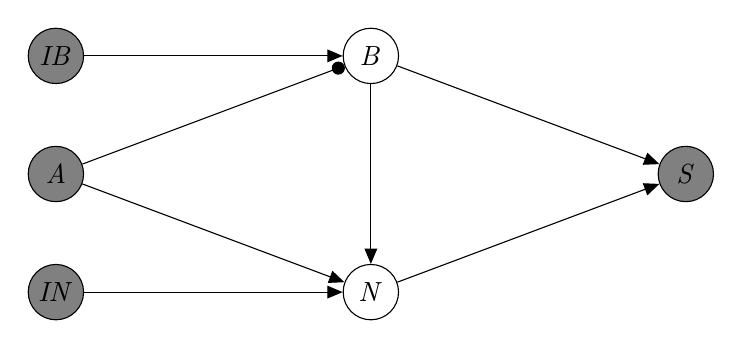
\begin{tikzpicture}
  \tikzset{neuron/.style = {shape=circle,draw,minimum size=2em,inner sep=1pt}}
    \tikzset{fireneuron/.style = {shape=circle,draw,minimum size=2em,inner sep=1pt, fill=gray}}
        \tikzset{sneuron/.style = {shape=circle,draw,minimum size=2em,inner sep=1pt, double, double distance=0.2mm}}
    \tikzset{sfireneuron/.style = {shape=circle,draw,minimum size=2em,inner sep=1pt, fill=gray,double, double distance=0.2mm}}
  \tikzset{edge/.style = {->,> = latex'}}
  \tikzset{%
  tipA/.tip={Triangle[angle=45:6pt]},
    tipB/.tip={Square[angle=45:6pt]},
}

	\node[fireneuron] (AF) at (0,1.5) {$\mathit{A}$};
	\node[fireneuron] (B) at (0,3) {$\mathit{IB}$};
	\node[fireneuron] (IN) at (0,0) {$\mathit{IN}$};
	
	\node[neuron] (BF) at (4,3) {$\mathit{B}$};
	
	\node[neuron] (N) at (4,0) {$\mathit{N}$};
	\node[fireneuron] (WS) at (8,1.5) {$\mathit{S}$};
	
    \foreach \from/\to in {AF/BF}
    \path[-*](\from) edge node [above]{} (\to);
    
    \foreach \from/\to in {AF/N, N/WS, BF/N, BF/WS, B/BF, IN/N}
    \path[-tipA](\from) edge node [above]{} (\to);
    
%        \foreach \from/\to in {AF/BF, AF/N}
%    \path[-tipB](\from) edge node [above]{} (\to);

\end{tikzpicture}
\end{center}


\parencite{beckers2018principled} takes a different approach. They argue that this issue has its origins in conflating early preemption and switching. 
That is, if Alice adds the antidote, then Bob will add poison to the the water, which promptly is neutralised allowing Carol to live on.
Otherwise, Bob will not add poison to the water and Carol will be unscathed. Hence, the actions of Alice are immaterial to the well-being of Carol.
Therefore, this example should be modelled as an instance of switch. Thereby, realigning structure with intuition.



Given the formalisation found in Example \ref{ex:short-circuit-0} both \hpu and \hpm declare the addition of the antidote to be the cause of Carol's survival \parencite[p.~90]{halpern2016actual}. 
The definition \ptc arrives at the same conclusion \parencite{weslake2015partial}.  
As already mentioned  in \parencite{beckers2018principled} Example \ref{ex:short-circuit-0} is deemed to be a switch variant. Therefore, their formalism, i.e.\ \bvcm, is constructed in such a manner that adding the antidote is immaterial for Carol's survival.


%\newcommand{\hpu}{\texttt{HP-05 }}
%\newcommand{\ptc}{\texttt{PTC}}
%\newcommand{\hpm}{\texttt{HP-15 }}
%\newcommand{\hpuc}{\texttt{HP-05c }}
%\newcommand{\bvcm}{\texttt{BV-CM}}
%\newcommand{\bci}{\texttt{BCI}}
%\newcommand{\scacc}{\texttt{SC-ACC}}
%\newcommand{\pcps}{\texttt{PCPS}}
%\newcommand{\at}{\texttt{AT}}
%\newcommand{\sccf}{\texttt{SC-CF}}

In \parencite{baumgartner2013regularity} another structure is classified under the umbrella of short circuit.
Example \ref{ex:short-circuit-1} labels the structure taken from \parencite{baumgartner2013regularity} to operate (roughly) within the narrative presented in Example \ref{ex:short-circuit-0}.


\begin{example}(Careful Poisoning)
\label{ex:short-circuit-1}
Carol lives ($CL$)
Alice puts a harmless antidote in Carol's water ($AA$). 
Adding antidote to the water, protects it against poison ($WS$ - ``water save'')
If Alice puts the antidote into Carol's water, Bob will poison the water ($BP$)
Adding poison to an unprotected water makes it toxic ($WT$).
If Carol would drink toxic water she would die (i.e.\ inhibiting $CS$).
Carol drinks her water and survives ($CS$).
%
%Seeing that the water contains an antidote Bob adds the poison into the water ($B$ - $B$ holds if Bob does not administer the poison). 
%This poison is countered by the antidote.  
%Carol drinks the water and survives ($CS$).
%Bob then poisons the water ($B$ - $B$ holds if Bob does not administer the poison), using a poison that is normally lethal, but which is countered by the antidote. Bob would not have poisoned the water if Alice had not administered the antidote first. Carol drinks the water and survives ($S$).
\begin{center}
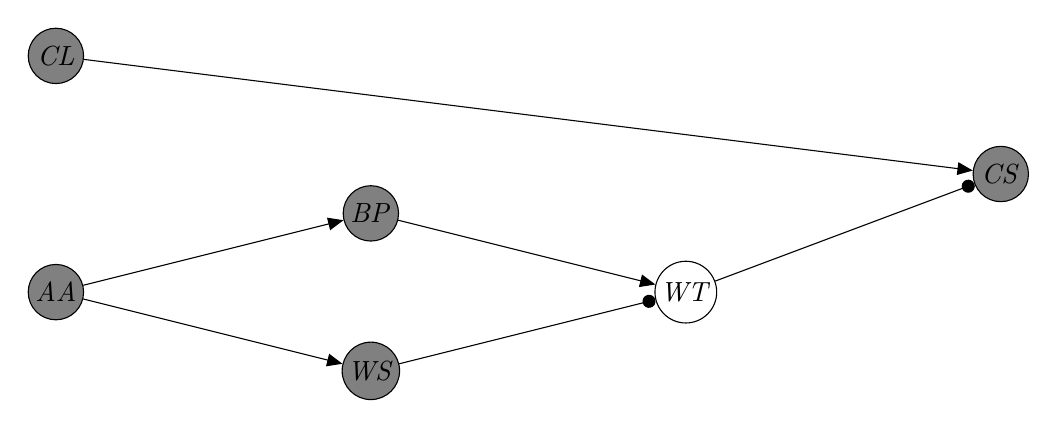
\begin{tikzpicture}
  \tikzset{neuron/.style = {shape=circle,draw,minimum size=2em,inner sep=1pt}}
    \tikzset{fireneuron/.style = {shape=circle,draw,minimum size=2em,inner sep=1pt, fill=gray}}
        \tikzset{sneuron/.style = {shape=circle,draw,minimum size=2em,inner sep=1pt, double, double distance=0.2mm}}
    \tikzset{sfireneuron/.style = {shape=circle,draw,minimum size=2em,inner sep=1pt, fill=gray,double, double distance=0.2mm}}
  \tikzset{edge/.style = {->,> = latex'}}
  \tikzset{%
  tipA/.tip={Triangle[angle=45:6pt]},
}

	\node[fireneuron] (A) at (0,4) {$\mathit{CL}$};
	\node[fireneuron] (C) at (0,1) {$\mathit{AA}$};
	
	\node[fireneuron] (D) at (4,2) {$\mathit{BP}$};
	\node[fireneuron] (B) at (4,0) {$\mathit{WS}$};
	
	\node[neuron] (F) at (8,1) {$\mathit{WT}$};
	
	\node[fireneuron] (E) at (12,2.5) {$\mathit{CS}$};
	
	

	
    \foreach \from/\to in {B/F, F/E}
    \path[-*](\from) edge node [above]{} (\to);
    
    \foreach \from/\to in {A/E, C/D,C/B, D/F}
    \path[-tipA](\from) edge node [above]{} (\to);

\end{tikzpicture}
\end{center}

\end{example}



\subsection{Other Examples}

\begin{example}
\label{ex:trumping-1}
There are a left and a right window.
Alice and Bob both order Carol to fire at the left window. Carol fires at the left window, shattering it. 
Commands from Alice always trump commands form Bob (e.g.\ if Bob would have ordered to fire at right window, Carol would still have fired at the left one.). 
Without a command Carol would not have fired at all.
What caused the left window to shatter?
\end{example}
Example \ref{ex:trumping-1} is a reformulation of the canonical example found in \parencite{halpern2011actual,weslake2015partial}.  
It was constructed to demonstrate the phenomena of trumping causation, which is elaborated on in XXXX.
Here intuitions conflict whether one should consider Alice alone, both individually or Alice and Bob as a conjunction to be the cause of the left window shattering \parencite{halpern2011actual,weslake2015partial}.




\begin{example}[\cite{halpern2015graded}]
\label{ex:omission-1}
If there is hot weather, flowers will die. Watering prevents the flowers to die in hot weather. The neighbour does not water the flowers. 
The flowers die. What caused the flowers to die?
\end{example}

Example \ref{ex:omission-1} is commonly used to discuss whether omissions should be considered as causes or not.
Here in particular, is the demise of the flowers the cause of the neighbour dying? While at first glance intuition would side for ``yes'', the discussion in XXXXX indicates that this question is not as straight forward as it may seem.
Some articles discussing the topic of omission and/or presenting its canonical examples similar to Example  \ref{ex:omission-1} are \parencite{glymour2010actual,halpern2011actual,halpern2015graded,blanchard2017cause}

\begin{example}[\cite{halpern2011actual}]
\label{ex:omission-2}
Suppose that Billy is hospitalized with a mild illness on Monday; he is treated and recovers. In the obvious causal model, the doctor’s treatment is a cause of Billy’s recovery. Moreover, if the doctor does not treat Billy on Monday, then the doctor’s omission to treat Billy is a cause of Billy’s being sick on Tuesday. But now suppose that there are 100 doctors in the hospital. Although only doctor 1 is assigned to Billy (and he forgot to give medication), in principle, any of the other 99 doctors could have given Billy his medication. Is the nontreatment by doctors 2–100 also a cause of Billy’s being sick on Tuesday?
\end{example}

For the sake of completion, Example \ref{ex:omission-2} is another common example used for discussing causation. It is a slight extension of Example \ref{ex:omission-1}.



\begin{example}[\cite{halpern2015graded}]
\label{ex:norms-1}
 The receptionist in the philosophy department keeps her desk stocked with pens. The administrative assistants are allowed to take pens, but faculty members are supposed to buy their own. The administrative assistants typically do take the pens. Unfortunately, so do the faculty members. The receptionist repeatedly e-mailed them reminders that only administrators are allowed to take the pens. On Monday morning, one of the administrative assis- tants encounters professor Smith walking past the receptionists desk. Both take pens. Later, that day, the receptionist needs to take an important message...but she has a problem. There are no pens left on her desk.
 \end{example}
 
Example \ref{ex:norms-1}, can be found in \parencite{beckers2016general,halpern2015graded}, is an example that demonstrates how norms influence causal attribution.
For a proper discussion about normality, norms and causation see XXXX.
In this example, intuition would dictate that professor Smith caused the absence of pens. This intuition was empirically tested and confirmed in \parencite{knobe2008causal}.

\begin{example}[\cite{halpern2015graded}]
\label{ex:background-1}
Consider a fire that is caused by a lit match. While the fire would not have occurred without the presence of oxygen in the atmosphere, the oxygen is deemed to be a background condition, rather than a cause.
 \end{example}

Example \ref{ex:background-1} is presented to discuss whether and how one should distinguish between causes and background conditions, a discussion held in XXXX.
Depending on the position taken in this discussion, one would either accept or deny the presence of oxygen the status of cause \parencite{halpern2015graded}.

\begin{example}[\cite{halpern2015graded}]
\label{ex:damping-1}
A lit match aboard a ship caused a cask of rum to ignite, causing the ship to burn, which resulted in a large financial loss by Lloyd’s insurance, leading to the suicide of a financially ruined insurance executive. The executive’s widow sued for compensation, and it was ruled that the negligent lighting of the match was not a cause (in the legally relevant sense) of his death.
 \end{example}

The answer whether the sailor dropping a lit match should be charged with being the cause of another persons death is yet again uncertain.
Due to its long causal chain, the cause is so far removed from the effect that intuition would disagree with a complete causal attribution. Hence, Example\ref{ex:damping-1} is well suited for highlighting issues with transitivity and binary causal attribution \parencite{halpern2015graded}. For a more detailed discussion see XXXXX.



\begin{example}[\cite{glymour2010actual}]
\label{ex:transitivity-1}
A boulder slides toward a hiker, who, seeing it, ducks. The boulder misses him and he survives. Did the boulder sliding cause his survival?
 \end{example}
 
Clearly, intuition would dictate that the boulder is not the cause of the hikers survival.
Hence, switching not the only example cited, when it comes to discussing the transitivity of causality. In particular, Example \ref{ex:transitivity-1} is the second example used in \parencite{hitchcock2001intransitivity}
to demonstrate that causation is not transitive (see XXXX). 


\begin{example}[\cite{blanchard2017cause}]
\label{ex:contrastive-1}
Consider a case where Doctor can administer no dose, one dose, or two doses of medicine to Patient. Patient will fail to recover if no dose is administered, but will recover if either one or two doses are administered. Let us suppose that Doctor in fact administers two doses, and Patient recovers.
 \end{example}
 
In \parencite{blanchard2017cause} Example \ref{ex:contrastive-1} was used to argue that causation should be considered as contrastive. 
This example is designed to provide different intuition about causation, depending on which possible scenario is used to counterfactually contrast the actual scenario against \parencite{blanchard2017cause}.
For further discussion see XXXX.


  
 \begin{example}[\cite{weslake2015partial}]
\label{ex:load-1}
A firing squad consists of shooters B and C. It is A’s job to load B’s gun, C loads and fires his own gun. On a given day, A loads B’s gun. When the time comes, only C shoots the prisoner.
 \end{example}
 
Example \ref{ex:load-1} is relative common, being discussed in \parencite{weslake2015partial,chockler2015causal,halpern2016appropriate,bochman2018actual}.
It is of particular relevance, as it was this example that lead to a reformulation of \hpo. While \hpo struggled with this example, its successor \hpu was able to match the intuitive answer that 
$C$ was the one causing the prisoners death.
However, \parencite{halpern2016appropriate} demonstrated that with proper modelling \hpo can achieve the same inferences as \hpu on this example.


 \begin{example}[\cite{blanchard2017cause}]
\label{ex:contrastive-1}
Consider a case where Doctor can administer no dose, one dose, or two doses of medicine to Patient. Patient will fail to recover if no dose is administered, but will recover if either one or two doses are administered. Let us suppose that Doctor in fact administers two doses, and Patient recovers.
 \end{example}
 
This example is used in \parencite{blanchard2017cause} to argue that causation is contrastive, i.e.\ the causal status of a variable depends on the variable it is contrasted against.
Here in particular, giving the patient two doses rather than zero doses caused the patient to recover. However, administering two doses rather than one dose did not cause the patient to recover.
XXXXX

\begin{example}
\label{ex:time-1}
Alice plans to go camping in June ($AC$). If there is a forest fire in May ($FF_m$), Alice will not go camping.
If Alice goes camping, she will cause a forest fire ($FF_j$).
\end{example}
%
%In \parencite{halpern2011actual}, the following formalisation is advised.
%\emph{Causal Model}
%
%\begin{equation*}
%\begin{split}
%& AC := \neg FF_m, \quad FF_j := AC \land \neg FF_m
%\end{split}
%\end{equation*}
%
%\emph{Neuron Diagram XXX}
%\begin{center}
%\begin{tikzpicture}
%  \tikzset{neuron/.style = {shape=circle,draw,minimum size=2em,inner sep=1pt}}
%    \tikzset{fireneuron/.style = {shape=circle,draw,minimum size=2em,inner sep=1pt, fill=gray}}
%      \tikzset{switch/.style = {shape=rectangle,draw,minimum size=2em,inner sep=1pt}}
%    \tikzset{fireswitch/.style = {shape=rectangle,draw,minimum size=2em,inner sep=1pt, fill=gray}}
%        \tikzset{sneuron/.style = {shape=circle,draw,minimum size=2em,inner sep=1pt, double, double distance=0.2mm}}
%    \tikzset{sfireneuron/.style = {shape=circle,draw,minimum size=2em,inner sep=1pt, fill=gray,double, double distance=0.2mm}}
%  \tikzset{edge/.style = {->,> = latex'}}
%  \tikzset{%
%  tipA/.tip={Triangle[angle=45:6pt]},
%}
%
%
%	\node[fireswitch] (AC) at (0,1) {$\mathit{AF}$};
%	\node[fireneuron] (TA) at (4,2) {$\mathit{TA}$};
%	\node[neuron] (TB) at (4,0) {$\mathit{TB}$};
%	
%	\node[fireneuron] (TD) at (8,1) {$\mathit{TD}$};
%	
%    \foreach \from/\to in {}
%    \path[-*](\from) edge node [above]{} (\to);
%    
%    \foreach \from/\to in {AF/TA, AF/TB, TB/TD, TA/TD}
%    \path[-tipA](\from) edge node [above]{} (\to);
%
%\end{tikzpicture}
%\end{center}
Example \ref{ex:time-1},  taken from \parencite{halpern2011actual}, stirs one directly into a meta-physical discussion about the nature of events. 
Meaning if the occurrence of an event is delayed, is it still the same event. Neglecting this distinction during the modelling process may result in undesirable results.
That is, if one would not have explicitly distinguished between the forest fire in May and the forest fire in June by using separate variables, the model would contain circularities and would allow for counter-intuitive inferences, e.g.\ creating a forest fire in June causes Alice to go camping \parencite{halpern2011actual}.  
XXXX
 
 \begin{example}[\cite{blanchard2017cause}]
\label{ex:wildwest-1}
A ranch has five individuals: Cowboy $C$, Ranger $R$, Wrangler $W$, and two Hands $H_1$, $H_2$. Everyone votes either for staying around the campfire ($0$), or for going on a round-up ($1$). A complicated rule is used to decide the outcome $O$: 
\begin{enumerate}
\item if $C = R$, then $O = R$,
\item if $R$ differs from the other four, then $O = R$,
\item otherwise, majority rules.
\end{enumerate}
Suppose $C = R = 1$ and $W = H_1 = H_2 = 0$ (and so $O = 1$). Was $W = 0$ an actual cause of $O = 1$?
 \end{example}




% A, an imperfect marksman, is about to fire at the target, but his aim is too low. B standing at the back of the crowd, could push his way through to A and lift the rifle barrel just the right amount, but B does no such thing. A’s bullet misses the bullseye. What caused the bullseye to be missed (D = 0)?
%
%Maybe!!!
%
%Consider the following story, taken from (an early version of) [Hall 2004]: Suppose that Billy is hospitalized with a mild illness on Monday; he is treated and recovers. In the obvious causal model, the doctor’s treatment is a cause of Billy’s recovery. Moreover, if the doctor does not treat Billy on Monday, then the doctor’s omission to treat Billy is a cause of Billy’s being sick on Tuesday. But now suppose that there are 100 doctors in the hospital. Although only doctor 1 is assigned to Billy (and he forgot to give medication), in principle, any of the other 99 doctors could have given Billy his medication. Is the nontreatment by doctors 2–100 also a cause of Billy’s being sick on Tuesday?
%
%
%. H=1 if the weather is hot, 0 if it is cool;
%. W =1 if the neighbour waters the flowers, 0 otherwise;
%. D=1 if the flowers die, 0 if they do not.
%There is one equation:
%D = H x (1-W)


%\subsection{Knobe Effects 28}

%
%Example 5. The receptionist in the philosophy department keeps her desk stocked with pens. The administrative assistants are allowed to take pens, but faculty members are supposed to buy their own. The administrative assistants typically do take the pens. Unfortunately, so do the faculty members. The receptionist repeatedly e-mailed them reminders that only administrators are allowed to take the pens. On Monday morning, one of the administrative assis- tants encounters professor Smith walking past the receptionists desk. Both take pens. Later, that day, the receptionist needs to take an important message...but she has a problem. There are no pens left on her desk.
%
% 


%\subsection{Causes and Background Conditions 39}
%A standard example is a fire that is caused by a lit match. While the fire would not have occurred without the presence of oxygen in the atmosphere, the oxygen is deemed to be a background condition, rather than a cause.
%
%
%We have three variables:
%. M=1 if the match is lit, 0 otw;
%. O = 1 if oxygen is present, 0 if there is no oxygen;
%. F =1 if there is a fire, 0 if there is no fire. There is one equation:
%F=min(M,O)
%

%\subsection{Causal Chain}

%
% [Causal Chains] -> Transitity?
%(Graded Causation?)
%
%For example, in Regina v. Faulkner ([1877]), a well-known Irish case, a lit match aboard a ship caused a cask of rum to ignite, causing the ship to burn, which resulted in a large financial loss by Lloyd’s insurance, leading to the suicide of a financially ruined insurance executive. The executive’s widow sued for compensation, and it was ruled that the negligent lighting of the match was not a cause (in the legally relevant sense) of his death.
%
%M=1ifthematchislit,0ifitisnot;
%. R=1ifthereisruminthevicinityofthematch,0ifnot;
%. RI =1iftherumignites,0ifitdoesnot;
%. F = 1 if there is further flammable material near the rum, 0 if not;
%. SD = 1 if the ship is destroyed, 0 if not;
%. LI = 1 if the ship is insured by Lloyd’s, 0 if not;
%. LL = 1 if Lloyd’s suffers a loss, 0 if not;
%. EU = 1 if the insurance executive was mentally unstable, 0 if not;
%. ES = 1 if the executive commits suicide, 0 if not.
%
%RI = min(M,R)
%SB = min(RI,F)
%LL = min(SB, LI)
%ES = min(LL,EU)

%\subsection{Contrastive Causality 43}

%To illustrate the plausibility of the view that actual causation is contrastive, consider a case where Doctor can administer no dose, one dose, or two doses of medicine to Patient. Patient will fail to recover if no dose is administered, but will recover if either one or two doses are administered. Let us suppose that Doctor in fact administers two doses, and Patient recovers. It would be natural to model this causal scenario using a ternary variable M, which takes value 0, 1, or 2 according to whether Doctor administers 0, 1, or 2 doses of medicine, and a binary variable, R, which takes value 0 if Patient fails to recover and 1 if she recovers. We can also add an exogenous variable, I, which takes value 0 if Doctor intends to administer zero doses, 1 if Doctor intends to administer one dose, and 2 if Doctor intends to administer two doses. The three structural equations for this case are then I 1⁄4 2, M 1⁄4 I, and R 1⁄4 M=MaxfM;1g. The actual solution is I1⁄42, M1⁄42, and R1⁄41.


%\subsection{Boulder}

% A boulder slides (B = 1) toward a hiker, who, seeing it, ducks (D = 1). The boulder misses him and he survives (S = 1). Did the boulder sliding cause his survival?
%

%\subsection{Wild West}
%
%%A ranch has five individuals: Cowboy C, Ranger R, Wrangler W, and two Hands H1, H2. Everyone votes either for staying around the campfire (0), or for going on a round-up (1). A complicated rule is used to decide the outcome O: (a) if C = R, then O = R; (b) if R differs from the other four, then O = R; and (c) otherwise, majority rules. Suppose C = R = 1 and W = H1 = H2 = 0 (and so O = 1). Was W = 0 an actual cause of O = 1?
%%
%%
%
%\subsection{Shock}
%%Two two-state switches are wired to an electrode. e switches are controlled by A and B respectively, and the electrode is attached to C. A has the first option to flip her switch (A = 1). B has the second option to flip her switch (B = 1). e electrode is activated and shocks C (C = 1) iff both switches are in the same position. B wants to shock C, and so flips her switch iff A does.

%\subsection{Push}

%[Push]
%I push(P=1)Jonesinfrontofatruck(T =1),whichhits(H=1)andkills him(D = 1);ifIhadnotdoneso(P = 0),abus(B = 1)wouldhavehit (H = 1) and killed him.
%
%Version (A): re is no other action available.
%Version (B): I can push (P = 2) Jones to safety (H = 0).

%\subsection{Loader}

%A firing squad consists of shooters B and C. It is A’s job to load B’s gun, C loads and fires his own gun. On a given day, A loads B’s gun. When the time comes, only C shoots the prisoner.
%A = 1; B=0; C=1
%D=(A and B) or C

%\subsection{Wall}
%
%SupposeIreachoutandcatchapassingcricketball. The next thing along in the ball’s direction of motion was a solid brick wall. Beyond that was a window.
%
%%\subsection{Garden}

%
%. H=1 if the weather is hot, 0 if it is cool;
%. W =1 if the neighbour waters the flowers, 0 otherwise;
%. D=1 if the flowers die, 0 if they do not.
%There is one equation:
%D = H x (1-W)




\section{Properties of Causation}

\subsection{Redundant Causation}


\subsection{Transitive Causation}

\subsection{Normality, Norms and Causation}
%775 argument agains normality (switch)
\subsection{Contrastive Causation}

\subsection{Time and Causation}

\subsection{Certainty, Probability and Non-determinism}

\subsection{Trumping Causation}
%17

%
%Suppose that a group of soldiers is very well trained, so that they will obey any order given by a superior officer; in the case of conflicting orders, they obey the
%highest-ranking officer. Both a sergeant and a major issue the order to march, and the soldiers march
%
%
%Major (M) and and sergeant (S) stand before corporal, and both shout ‘Charge!’ (M = 1, S = 1). e corporal charges (C = 1). Orders from higher- ranking soldiers trump those of lower rank, so if the major had shouted ‘Halt’ (M = 2) the corporal would not have charged.

Trumping is discussed in \parencite{halpern2011actual,weslake2015partial}.
According to \parencite{weslake2015partial}, this example is rather contentions. 
Not only is there disagreements about what should be intuitively understood as a cause,
but also the relationship of trumping causation with respect of other forms of causation, in particularly with symmetric overdetermination and preemption, is subject to a lively debate.
As indicated by the name one speaks of trumping, if one causal process always dominates the other. 
That is, if the process $A$ is active, process $B$ is irrelevant for the status of $C$.
However, if process $A$ is inactive, the status of $C$ depends on $B$.

This scenario presented in Example \ref{ex:trumping-1} shares clearly shares similarities with both symmetric overdetermination and late preemption. 
That is, similar to late preemption Bob's command starts a process that is ``interrupted'' by Alice's command.
However, in this particular case the given commands are identical and are issues at the exact same moment, allowing one to draw a similarity to switching.
\parencite{hitchcock2011trumping} argues that this example has  far reaching implications for the taxonomy of redundant causation. 
He claims that this example can not be classified as either symmetric overdetermination or preemption. 
Hence, contradicting the belief that redundant causation is characterised by this dichotomy. 

Particularly interesting is that in order to relegate the causal attribution in Example \ref{ex:trumping-1} to Alice and Bob alone, one must accept that Carol is void of agency.
Practically operating as a robot, as otherwise some responsibility must be attributed to Carol as well. Therefore, it is critical to include this piece of information in Example \ref{ex:trumping-1} preventing hidden 
assumptions, in this case the agency of people, to tarnish the causal intuition.
This highlights that using such stories as a foundation for constructing causation may be problematic.


\subsection{Causation by Omission}
\label{subsec:omission}
Causation by omission, is the claim that the non occurrence of an event caused another event, e.g.\ $\neg A$ caused $B$.
However, this is a contentions topic. Not only does \parencite{blanchard2017cause} claim that causation by omission is one of the open problems in determining actual causation.
It is also the case, there remains disagreement within the literature of whether causation by omission should be considered when defining token causality.
\parencite{halpern2015graded} identified four established viewpoints within this debate.
The first dismisses causation by omission, while the second completely embraces it. 
The third, is positioned somewhere in between, declaring omissions to have some kind of secondary status.
The last argues that it is the normative status of an omission that determines its causal status, e.g.\ in Example \ref{ex:omission-1}
the inaction of the neighbour only caused the death of the flowers, if he had the obligation to do so.


When assessing Example \ref{ex:omission-1} 
A person inclined to attribute the neighbours omission as the cause of the flower's demise, may have incorporated some implicit assumption into their reasoning process.
Because, as described in the example the neighbour has no obligation to water the flowers. Meaning, without a statement such as ``The neighbour was responsible to water the flowers'', the neighbour
is on equal footing with any other person in this world. 
One suggestion, would be to appeal to normality. That is, expecting the neighbour to water the flowers is considered less out of the ordinary that expecting some person on the other side of the world to do so.
An additional benefit of this approach is that it provides sufficient flexibility to accommodate all the previously listed viewpoints. 
However, this flexibility can be problematic, as one has to rank scenarios based on their perceived normality. For example, what if the neighbour was gardener, but also is sworn to kill this particular kind of flowers. Is the scenario now more or less normal?
To avoid the reliance on normality, one could also argue for the restriction of the models used. Limiting the variables used to only those relevant (seemingly) relevant for the scenario.
For Example \ref{ex:omission-1} this would imply that only the neighbour and no other person is relevant for the status of the flowers \parencite{blanchard2017cause}.




\chapter{Token Causal Definitions: A comparison}
\chaptermark{Token Causal Definitions}
\label{ch:literature_review}

\section{Token Causal Definitions}
\subsection{Modified Halpern and Pearl Definition}

\subsection{Bochmans Causal Inference}

\subsection{Possible Causal Processes}


\section{Comparison}


The important publications as contained in $\prset$ (see Subsection \ref{subsec:important_pubs}) rely on a variety of languages to encode causal relations. Table \ref{tab:language} provides insight into which publications discuss which language family.
However, it must be remarked that some liberty with respect to aggregation was taken, e.g.\ causal models with and without defaults are considered part of the same language family. 
Here it is important to point out that by far the most discussed framework are causal models, with CP-Logic and Causal Logic tying for a distant second place. 


\begin{sidewaystable}
\centering
\tiny
\begin{tabular}{lp{1cm}p{1cm}p{1cm}p{1cm}p{1cm}p{1cm}p{1.1cm}p{1cm}p{1cm}p{1cm}p{1cm}}
\toprule
Articles & Causal Models	& CP-Logic	& Situation Calculus	&  Non-Monotonic Causal Theory & FOL & Neuron Diagrams & 	Conditional Logic	& $\mathcal{AL}$	& SFCA &  Abductive Causal Theory \\   
\midrule        
\cite{vennekens2010embracing} 	& 	& X	& 	& 	& 	& 	& 	& 	& 	& 	\\
 \cite{bex2010hybrid} 	& 	& 	& 	& 	& 	& 	& 	& 	& 	& X	\\
 \cite{lee2010representing}	& 	& 	& 	& X	& 	& 	& 	& 	& 	& 	\\
 \cite{lifschitz2010translating} 	& 	& 	& 	& X	& 	& 	& 	& 	& 	& 	\\
 \cite{glymour2010actual}	& X	& 	& 	& 	& 	& X	& 	& 	& 	& 	\\
 \cite{claassen2010causal} 	& X	& 	& 	& 	& 	& 	& 	& 	& 	& 	\\
 \cite{gerstenberg2010spreading}	& X	& 	& 	& 	& 	& 	& 	& 	& 	& 	\\
 \cite{halpern2011actual} 	& X	& 	& 	& 	& 	& 	& 	& 	& 	& 	\\
 \cite{shulz2011if} 	& X	& 	& 	& 	& 	& 	& 	& 	& 	& 	\\
 \cite{briggs2012interventionist}	& X	& 	& 	& 	& 	& 	& 	& 	& 	& 	\\
 \cite{baumgartner2013regularity} 	& 	& 	& 	& 	& X	& X	& 	& 	& 	& 	\\
 \cite{hyttinen2013discovering} 	& X	& 	& 	& 	& 	& 	& 	& 	& 	& 	\\
 \cite{halpern2015graded} 	& X	& 	& 	& 	& 	& 	& 	& 	& 	& 	\\
 \cite{weslake2015partial} 	& X	& 	& 	& 	& 	& 	& 	& 	& 	& 	\\
 \cite{chockler2015causal}  	& X	& 	& 	& 	& 	& 	& 	& 	& 	& 	\\
 \cite{beckers2016general} 	& 	& X	& 	& 	& 	& X	& 	& 	& 	& 	\\
 \cite{schaffer2016grounding}  	& X	& 	& 	& 	& 	& 	& 	& 	& 	& 	\\
 \cite{halpern2016appropriate} 	& X	& 	& 	& 	& 	& 	& 	& 	& 	& 	\\
 \cite{blanchard2017cause}  	& X	& 	& 	& 	& 	& 	& 	& 	& 	& 	\\
 \cite{wright2017ness}  	& 	& 	& 	& 	& 	& 	& 	& 	& 	& 	\\
 \cite{icard2017normality} 	& 	& 	& 	& 	& 	& 	& 	& 	& 	& 	\\
 \cite{aleksandrowicz2017computational}  	& X	& 	& 	& 	& 	& 	& 	& 	& 	& 	\\
 \cite{fenton2017proposed}  	& 	& 	& 	& 	& 	& 	& 	& 	& 	& 	\\
 \cite{lagnado2017causation}  	& X	& 	& 	& 	& 	& 	& 	& 	& 	& 	\\
 \cite{bochman2018actual}  	& X	& 	& 	& X	& 	& 	& 	& 	& 	& 	\\
 \cite{ibeling2018conditional}  	& 	& 	& 	& 	& 	& 	& X	& 	& 	& 	\\
 \cite{beckers2018principled} 	& X	& 	& 	& 	& 	& 	& 	& 	& 	& 	\\
 \cite{bochman2018laws}  	& X	& 	& 	& X	& 	& 	& 	& 	& 	& 	\\
 \cite{denecker2018causal}  	& 	& X	& 	& 	& 	& 	& 	& 	& 	& 	\\
 \cite{batusov2018situation}  	& X	& 	& X	& 	& 	& 	& 	& 	& 	& 	\\
 \cite{denecker2019explaining}  	& X	& X	& 	& 	& 	& 	& 	& 	& 	& 	\\
 \cite{liepicna2019evaluation}  	& 	& 	& 	& 	& 	& 	& 	& 	& X	& 	\\
 \cite{leblanc2019explaining} 	& 	& 	& 	& 	& 	& 	& 	& X	& 	& 	\\
 \cite{liepicna2020arguing} 	& X	& 	& 	& 	& 	& 	& 	& 	& X	& 	\\
 \cite{khannecessary}  	& X	& 	& X	& 	& 	& 	& 	& 	& 	& 	\\
 \cite{ibeling2020probabilistic}  	& X	& 	& 	& 	& 	& 	& X	& 	& 	& 	\\
\bottomrule
\end{tabular}
\caption{Depicts which publication discuss which languages families}
\label{tab:language}
\end{sidewaystable}


 

%
%
% \begin{sidewaystable}
%\centering
%\tiny
%\begin{tabular}{lp{0.3cm}p{0.3cm}p{0.3cm}p{0.3cm}p{0.3cm}p{0.3cm}p{0.3cm}p{0.3cm}p{0.3cm}p{0.3cm}p{0.3cm}p{0.2cm}p{0.05cm}p{0.05cm}p{0.1cm}p{0.3cm}p{0.3cm}p{0.3cm}p{0.2cm}p{0.1cm}p{0.1cm}p{0.3cm}p{0.3cm}p{0.3cm}p{0.3cm}p{0.3cm}p{0.3cm}p{0.3cm}p{0.3cm}p{0.3cm}p{0.3cm}p{0.3cm}p{0.3cm}p{0.3cm}p{0.3cm}}
%\toprule
%Articles & But-For & CRF & INUS & NESS & Hitch-01 & HP-01 & 	Wood-03	& Hall-04p	& Hall-04d & HP-05 & Hall-07 & HP-08d & S & SJ & BV-11 &  BV-12 &  B-Reg &
%PTC &  HH-CP & HM & MM & BV-CM & BCI & SC-ACC & PCPS & AT & SC-CF & CAEC \\
%\\   
%\midrule        
%\cite{vennekens2010embracing} & 	& 	& 	& 	& 	& 	& 	& 	& 	& 	& 	& 	& 	& 	& 	& 	& 	& 	& 	& 	& 	& 	& 	& 	& 	& 	& 	& 	\\
% \cite{bex2010hybrid} & 	& 	& 	& 	& 	& 	& 	& 	& 	& 	& 	& 	& 	& 	& 	& 	& 	& 	& 	& 	& 	& 	& 	& 	& 	& 	& 	& 	\\
% \cite{lee2010representing} & 	& 	& 	& 	& 	& 	& 	& 	& 	& 	& 	& 	& 	& 	& 	& 	& 	& 	& 	& 	& 	& 	& 	& 	& 	& 	& 	& 	\\
% \cite{lifschitz2010translating} & 	& 	& 	& 	& 	& 	& 	& 	& 	& 	& 	& 	& 	& 	& 	& 	& 	& 	& 	& 	& 	& 	& 	& 	& 	& 	& 	& 	\\
% \cite{glymour2010actual}& 	& 	& 	& 	& 	& 	& X	& 	& 	& X	& 	& 	& X	& X	& 	& 	& 	& 	& 	& 	& 	& 	& 	& 	& 	& 	& 	& 	\\
% \cite{claassen2010causal} & 	& 	& 	& 	& 	& 	& 	& 	& 	& 	& 	& 	& 	& 	& 	& 	& 	& 	& 	& 	& 	& 	& 	& 	& 	& 	& 	& 	\\
% \cite{gerstenberg2010spreading} & X	& 	& 	& 	& 	& 	& 	& 	& 	& X	& 	& 	& 	& 	& 	& 	& 	& 	& 	& 	& 	& 	& 	& 	& 	& 	& 	& 	\\
% \cite{halpern2011actual} & 	& 	& 	& 	& 	& 	& 	& 	& 	& X	& 	& X	& 	& 	& 	& 	& 	& 	& 	& 	& 	& 	& 	& 	& 	& 	& 	& 	\\
% \cite{shulz2011if} & 	& 	& 	& 	& 	& 	& 	& 	& 	& 	& 	& 	& 	& 	& 	& 	& 	& 	& 	& 	& 	& 	& 	& 	& 	& 	& 	& 	\\
% \cite{briggs2012interventionist} & 	& 	& 	& 	& 	& 	& 	& 	& 	& 	& 	& 	& 	& 	& 	& 	& 	& 	& 	& 	& 	& 	& 	& 	& 	& 	& 	& 	\\
% \cite{baumgartner2013regularity} & 	& 	& X	& X	& 	& 	& 	& 	& 	& 	& 	& 	& 	& 	& 	& 	& X	& 	& 	& 	& 	& 	& 	& 	& 	& 	& 	& 	\\
% \cite{hyttinen2013discovering} & 	& 	& 	& 	& 	& 	& 	& 	& 	& 	& 	& 	& 	& 	& 	& 	& 	& 	& 	& 	& 	& 	& 	& 	& 	& 	& 	& 	\\
% \cite{halpern2015graded} & 	& 	& 	& 	& 	& 	& 	& 	& 	& X	& 	& X	& 	& 	& 	& 	& 	& 	& 	& 	& 	& 	& 	& 	& 	& 	& 	& 	\\
% \cite{weslake2015partial} & 	& 	& 	& 	& X	& X	& X	& 	& 	& X	& 	& 	& 	& 	& 	& 	& 	& X	& 	& 	& 	& 	& 	& 	& 	& 	& 	& 	\\
% \cite{chockler2015causal} & 	& 	& 	& 	& 	& 	& 	& 	& 	& X	& 	& 	& 	& 	& 	& 	& 	& 	& 	& 	& 	& 	& 	& 	& 	& 	& 	& 	\\
% \cite{beckers2016general} & 	& 	& 	& 	& 	& 	& 	& X	& X	& X	& X	& X	& 	& 	& X	& X	& 	& 	& X	& 	& 	& 	& 	& 	& 	& 	& 	& 	\\
% \cite{schaffer2016grounding} & 	& 	& 	& 	& 	& 	& 	& 	& 	& 	& 	& 	& 	& 	& 	& 	& 	& 	& 	& 	& 	& 	& 	& 	& 	& 	& 	& 	\\
% \cite{halpern2016appropriate} & 	& 	& 	& 	& 	& X	& 	& 	& 	& X	& 	& X	& 	& 	& 	& 	& 	& 	& 	& 	& 	& 	& 	& 	& 	& 	& 	& 	\\
% \cite{blanchard2017cause} & 	& 	& 	& 	& X	& 	& 	& 	& 	& 	& 	& 	& 	& 	& 	& 	& 	& 	& 	& X	& X	& 	& 	& 	& 	& 	& 	& 	\\
% \cite{wright2017ness} & X	& X	& X	& X	& 	& 	& 	& 	& 	& 	& 	& 	& 	& 	& 	& 	& 	& 	& 	& 	& 	& 	& 	& 	& 	& 	& 	& 	\\
% \cite{icard2017normality} & 	& 	& 	& 	& 	& 	& 	& 	& 	& 	& 	& 	& 	& 	& 	& 	& 	& 	& 	& 	& 	& 	& 	& 	& 	& 	& 	& 	\\
% \cite{aleksandrowicz2017computational} & 	& 	& 	& 	& 	& X	& 	& 	& 	& X	& 	& 	& 	& 	& 	& 	& 	& 	& 	& 	& 	& 	& 	& 	& 	& 	& 	& 	\\
% \cite{fenton2017proposed} & 	& 	& 	& 	& 	& 	& 	& 	& 	& 	& 	& 	& 	& 	& 	& 	& 	& 	& 	& 	& 	& 	& 	& 	& 	& 	& 	& 	\\
% \cite{lagnado2017causation} & 	& 	& 	& 	& 	& 	& 	& 	& 	& 	& 	& 	& 	& 	& 	& 	& 	& 	& 	& 	& 	& 	& 	& 	& 	& 	& 	& 	\\
% \cite{bochman2018actual} & 	& 	& 	& X	& 	& 	& 	& 	& 	& 	& 	& 	& 	& 	& 	& 	& 	& 	& 	& 	& 	& 	& X	& 	& 	& 	& 	& 	\\
% \cite{ibeling2018conditional} & 	& 	& 	& 	& 	& 	& 	& 	& 	& 	& 	& 	& 	& 	& 	& 	& 	& 	& 	& 	& 	& 	& 	& 	& 	& 	& 	& 	\\
% \cite{beckers2018principled} & 	& 	& 	& 	& 	& 	& 	& 	& 	& X	& 	& 	& 	& 	& 	& 	& 	& 	& 	& 	& 	& X	& 	& 	& 	& 	& 	& 	\\
% \cite{bochman2018laws} & 	& 	& 	& 	& 	& 	& 	& 	& 	& 	& 	& 	& 	& 	& 	& 	& 	& 	& 	& 	& 	& 	& X	& 	& 	& 	& 	& 	\\
% \cite{denecker2018causal} & 	& 	& 	& 	& 	& 	& 	& 	& 	& X	& 	& 	& 	& 	& 	& 	& 	& 	& 	& 	& 	& 	& 	& 	& X	& 	& 	& 	\\
% \cite{batusov2018situation} & 	& 	& 	& 	& 	& 	& 	& 	& 	& X	& 	& 	& 	& 	& 	& 	& 	& 	& 	& 	& 	& 	& 	& X	& 	& 	& 	& 	\\
% \cite{denecker2019explaining} & 	& 	& 	& 	& 	& 	& 	& 	& 	& 	& 	& 	& 	& 	& 	& 	& 	& 	& 	& 	& 	& 	& 	& 	& X	& 	& 	& 	\\
% \cite{liepicna2019evaluation} & 	& 	& 	& 	& 	& 	& 	& 	& 	& 	& 	& 	& 	& 	& 	& 	& 	& 	& 	& 	& 	& 	& 	& 	& 	& 	& 	& X	\\
% \cite{leblanc2019explaining}& 	& 	& 	& 	& 	& 	& 	& 	& 	& 	& 	& 	& 	& 	& 	& 	& 	& 	& 	& 	& 	& 	& 	& 	& 	& X	& 	& 	\\
% \cite{liepicna2020arguing} & X	& X	& 	& 	& 	& 	& 	& 	& 	& X	& 	& 	& 	& 	& 	& 	& 	& 	& 	& 	& 	& 	& 	& 	& 	& 	& 	& 	\\
% \cite{khannecessary} & 	& 	& X	& 	& 	& 	& 	& 	& 	& X	& 	& 	& 	& 	& 	& 	& 	& 	& 	& 	& 	& 	& 	& 	& 	& 	& X	& 	\\
% \cite{ibeling2020probabilistic} & 	& 	& 	& 	& 	& 	& 	& 	& 	& 	& 	& 	& 	& 	& 	& 	& 	& 	& 	& 	& 	& 	& 	& 	& 	& 	& 	& 	\\
%\bottomrule
%\end{tabular}
%\caption{Depicts which publication discuss which languages families}
%\label{tab:language}
%\end{sidewaystable}



%
%\cite{vennekens2010embracing} 	
% \cite{bex2010hybrid} 
% \cite{lee2010representing}
% \cite{lifschitz2010translating} 
% \cite{glymour2010actual}
% \cite{claassen2010causal} 
% \cite{gerstenberg2010spreading}
% \cite{halpern2011actual} 
% \cite{shulz2011if} 
% \cite{briggs2012interventionist}
% \cite{baumgartner2013regularity} 
% \cite{hyttinen2013discovering} 
% \cite{halpern2015graded} 
% \cite{weslake2015partial} 
% \cite{chockler2015causal}  
% \cite{beckers2016general} 
% \cite{schaffer2016grounding}  
% \cite{halpern2016appropriate} 
% \cite{blanchard2017cause}  
% \cite{wright2017ness}  
% \cite{icard2017normality} 
% \cite{aleksandrowicz2017computational}  
% \cite{fenton2017proposed}  
% \cite{lagnado2017causation}  
% \cite{bochman2018actual}  
% \cite{ibeling2018conditional}  
% \cite{beckers2018principled} 
% \cite{bochman2018laws}  
% \cite{denecker2018causal}  
% \cite{batusov2018situation}  
% \cite{denecker2019explaining}  
% \cite{liepicna2019evaluation}  
% \cite{leblanc2019explaining} 
% \cite{liepicna2020arguing} 
% \cite{khannecessary}  
% \cite{ibeling2020probabilistic}  


%
%\begin{itemize}
%
%\item CM Woodward
%\item CM HP 2001	
%\item CM HP 2005	
%\item CM HP 2005 + Normality	
%\item CM Hitchcock	
%\item Bochman Causal Inference
%\item Simulation Model
%\item Causal Process Semantics
%\item Achievment Causal Chain
%\item SFCA
%\end{itemize}




%\item But For 	
%\item INUS
%\item NESS	
%\item Hart


%\begin{itemize}
%
%\item CM Partial Theory	
%\item CM Hitchcock	
%\item CM Hitchcock meets Menzies	
%\item CM Menzies-by-Menzies	
%\item CM VB
%\item Hall 2007	Production	
%\item Dependence	
%\item BV12	
%\item HH-CP	
%\item FO Minimality	
%\item But For 	
%\item INUS
%\item NESS	
%\item Hart	
%\item Bochman Causal Inference
%\item Simulation Model
%\item Causal Processes
%\item Achievment Causal Chain
%\item AL
%\item SFCA
%\end{itemize}



%
%\begin{figure}[h]
%\includegraphics[width=\textwidth]{important_cgraph.png}
%\caption{XXXX}
%\label{fig:cgraph-important}
%\end{figure}
%
%\begin{figure}[h]
%\includegraphics[width=\textwidth]{important_acgraph.png}
%\caption{XXXX}
%\label{fig:acgraph-important}
%\end{figure}



%Structural Equations and Beyond generalises structural models
%
%Causality Checking for Complex System Models Event order logic


%
%\chapter{Computational Causality}
%\label{ch:comp_causality}
%

















%\section{Modelling Languages}
%
%To introduce some of the languages used to encode causal relationships a simple example is required. 
%\begin{example}
%\label{ex:causal_model_forrest_fire_1}
%Consider the following causal relation:
%\begin{itemize}
%\item Both a lightning strike ($\mathit{LS}$) or a dropped match ($\mathit{MD}$) can to cause a forest fire ($\mathit{FF}$).
%\end{itemize}
%\end{example}
%
%\begin{example}
%\label{ex:causal_model_forrest_fire_2}
%Consider the following causal relation:
%\begin{itemize}
%\item Both a lightning strike ($\mathit{LS}$) and a dropped match ($\mathit{MD}$) are required to cause a forest fire ($\mathit{FF}$).
%\end{itemize}
%%Was the forest fire ($\mathit{FF}$) caused by an arsonist dropping a lit match ($\mathit{MD}$), or be a lightning strike ($\mathit{LS}$).
%\end{example}
%
%\begin{example}
%\label{ex:causal_model_forrest_fire_3}
%Consider the following causal relations:
%\begin{itemize}
%\item A small fire ($\mathit{SF}$) causes a big fire ($\mathit{BF}$).
%\item A big fire ($\mathit{BF}$) causes a forest fire ($\mathit{FF}$).
%\item A thunderstorm ($\mathit{TS}$) causes rain fall ($\mathit{RF}$) and lightning strikes ($\mathit{LS}$).
%\item Lightning  ($\mathit{LS}$) strikes cause big fires  ($\mathit{BS}$)
%\item Rainfall ($\mathit{RF}$) prevents small fires ($\mathit{SF}$).  
%\item Dropping a match ($\mathit{MD}$) causes a small fire ($\mathit{SF}$)
%\end{itemize}
%%Given a clear sky ($\mathit{CS}$), was the forest fire ($\mathit{FF}$) caused by an arsonist dropping a lit match ($\mathit{MD}$), or be a lightning strike ($\mathit{LS}$).
%%Both a lightning strike or the dropped match can cause the forest fire. However, no lightning can occur if the sky is blue. 
%\end{example}



%For purpose of this section, neural diagrams will be used as a useful method for striping the examples presented in this section down to their bare structure, permitting a clear comparison of the formalisms presented in Chapter \ref{ch:comp_causality}, based on which neurons they deem causal for the firing of another. 
%The disproportionate focus on causal models, seem to support the intuition that this particular formalism dominates the discussion, especially in the realm of token causality. This inference is further strengthened by the fact that the HP-2005 definition, which relies on causal models, is frequently used as a benchmark against which newer formalisms are tested against. This popularity, however, does not make it invulnerable to criticism. 
%Firstly, 
%
%\begin{example}
%Consider Example \ref{ex:causal_model_forrest_fire_3}. Assume that $\mathit{MD}$ and $\mathit{TS}$ fire. This results in the following diagram.
%\begin{center}
%\begin{tikzpicture}
%  \tikzset{neuron/.style = {shape=circle,draw,minimum size=2em,inner sep=1pt}}
%    \tikzset{fireneuron/.style = {shape=circle,draw,minimum size=2em,inner sep=1pt, fill=gray}}
%  \tikzset{edge/.style = {->,> = latex'}}
%  \tikzset{%
%  tipA/.tip={Triangle[angle=45:6pt]},
%}
%
%	\node[fireneuron] (MD) at (0,0) {$\mathit{MD}$};
%	
%	\node[neuron] (SF) at (4,0) {$\mathit{SF}$};
%	\node[fireneuron] (BF) at (8,0) {$\mathit{BF}$};
%	\node[fireneuron] (FF) at (12,0) {$\mathit{FF}$};
%	
%	\node[fireneuron] (TS) at (0,2) {$\mathit{TS}$};
%	\node[fireneuron] (LS) at (6,1) {$\mathit{LS}$};
%	\node[fireneuron] (RF) at (2,1) {$\mathit{RF}$};
%	
%	
%	 \path[-*] (RF) edge node [above]{} (SF);
%	 
%    \foreach \from/\to in {MD/SF, SF/BF, BF/FF, TS/LS, TS/RF, LS/BF}
%    \path[-tipA](\from) edge node [above]{} (\to);
%
%\end{tikzpicture}
%\end{center}
%Here it is clear to see that $\mathit{TS}$ and $\mathit{MD}$ are exogenous, while the remaining are endogenous. Moreover, the effect of $\mathit{MD}$ is cancelled, due to the fact that $\mathit{RF}$ fired.
%\end{example}
%
%
%
%\begin{example}
%Consider Example \ref{ex:causal_model_forrest_fire_2}. If one considers $\mathit{FF}$ to be a stubborn neuron, i.e.\ one that only fires, if all of its predecessors fire, then the causal relations presented can be encoded as the following neuron diagram.
%\begin{center}
%\begin{tikzpicture}
%  \tikzset{neuron/.style = {shape=circle,draw,minimum size=2em,inner sep=1pt}}
%    \tikzset{fireneuron/.style = {shape=circle,draw,minimum size=2em,inner sep=1pt, fill=gray}}
%    \tikzset{stubbornneuron/.style = {shape=circle,draw,minimum size=2em,inner sep=1pt, double, double distance=0.6mm}}
%    \tikzset{firestubbornneuron/.style = {shape=circle,draw,minimum size=2em,inner sep=1pt, fill=gray,double, double distance=0.6mm}}
%  \tikzset{edge/.style = {->,> = latex'}}
%  \tikzset{%
%  tipA/.tip={Triangle[angle=45:6pt]},
%}
%	
%	\node[fireneuron] (MD) at (0,0) {$\mathit{MD}$};
%	\node[neuron] (LS) at (0,2) {$\mathit{LS}$};
%	\node[firestubbornneuron] (FF) at (4,1) {$\mathit{FF}$};
%
%    \foreach \from/\to in {MD/FF, LS/FF}
%    \path[-tipA](\from) edge node [above]{} (\to);
%
%\end{tikzpicture}
%\end{center}
%\end{example}
%
%%
%The intuition conveyed above was both formalised and generalised in \cite{erwig2010causal}. To do so they destination between \emph{neuron graphs} capturing an abstract neuron structure and \emph{neuron diagrams} representing the execution of neuron graphs for some set of inputs. 
%For the subsequent definitions, let $\mathbb{F}_{\mathbb{B}}^{k,m}:= \{f \mid f:\mathbb{B}^k\to \mathbb{B}^m\}$ be the set of functions mapping $k$ boolean inputs to $m$ boolean outputs. 
%Let $\cbinfoos := \bigcup_{k>0} \mathbb{F}_{\mathbb{B}}^{k,1}$ be the set of all boolean functions. 

%\begin{definition}[\cite{erwig2010causal}]
%A \emph{neuron graph} is a directed acyclic graph $\ngraph:=(\cvars, \crel,\kappa, \sigma_{\cenvars})$, where $\cvars$ is the set of neurons and can be partitioned into endogenous variables $\cenvars$ and exogenous variables $\cexvars$; $\crel$ is a set of edges; $\kappa:V \to \{\text{§},!\}$ labels a neuron as either law or action; $\sigma_{\cenvars}:=\{ \sigma_v \mid \forall v \in \cenvars \; \sigma_v : \gtpred(v) \to \mathbb{B}\}$ is a set of functions mapping the predecessors of endogenous variables to a binary value.
%
% $\sigma_{\cenvars} : \cenvars \to \{f \mid f: \gtpred(v) \to \mathbb{B}\}$ maps every endogenous variable to an appropriate boolean function, i.e. for every $v \in \cenvars$ one has $\sigma_{\cenvars}(v): \cbinfoos^{\gtdegpred(v)} \to \mathbb{B}$. For $v \in \cvars$ let $\pi(v)$ be predefined ordering over $\gtpred(v)$.
%\end{definition}
%
%Moreover, from this one can build a neuron diagram by taking a neuron graph and providing an assignment of the exogenous variables.
%
%\begin{definition}[\cite{erwig2010causal}]
%Let $\ngraph:=(\cvars, \crel,\kappa, \sigma)$ be a neuron graph, then $\ndiagram:= (\ngraph, \sigma_{\cexvars}) $ is a \emph{neuron diagram} with  $\sigma_{\cexvars}: \cexvars \to \mathbb{B}$, i.e. 
%\end{definition}
%
%To evaluate such a neuron diagram, a firing semantic is required. 
%
%\begin{definition}[\cite{erwig2010causal}]



%
%%
%\subsection{Causal Models}
%\label{sec:causal_models}
%
%the version introduced, taken from \parencite{halpern2015cause}, was formulated in \cite{halpern2000axiomatizing}. However, \parencite{Weslake2015partial} slightly changed the notation to make the direction of such structural equations more apparent, thus this convention will be carried over into this work \parencite{halpern2015cause,Weslake2015partial}. 
%%
%% all relevant factors into a single exogenous variable. The value of this variable can provide the context necessary to explain the required background conditions for events to occur.
%%Using such a variable, one could also 
%%
%%
%%, e.g.\ this variable would explain all the conditions required for the lightning to strike or the arsonist to drop their match.  Moreover, the utility of $U$ can be further expanded upon, by allowing it to encode the relation between values, in this case it determines the value of $\mathit{FF}$ by allowing $U$ to determine the structural equation used, e.g.\ $\min$ or $\max$. As in Subsection \ref{subsec:neural_diagrams}, the variables of an causal model can be split into exogenous and endogenous variables. Depending on whether $U$ was used or not, either $U$ is exogenous and $\mathit{LS}$, $\mathit{MD}$ and $\mathit{FF}$ are endogenous or $\mathit{LS}$  and $\mathit{MD}$ exogenous and $\mathit{FF}$ is endogenous. Using the now cultivated intuition a formal definition can be given \cite{halpern2015cause}.
%%
%%
%%
%% Apart from being directed, another design choice made 
%% 
%% in this case $\mathit{FF}$,are best read as assignments rather than as a algebraic equation, in this case $\mathit{MD}$ and $\mathit{LS}$
%%  are best read as assignments rather than as a algebraic equation.
%%
%%
%%
%%
%%In \cite{halpern2015cause} Halpern introduces structural models using the following example.
%%
%%\begin{example}
%%\label{ex:causal_model_forrest_fire}
%%Consider Example \ref{ex:causal_model_forrest_fire_1}  and Example \ref{ex:causal_model_forrest_fire_2}.
%%In both cases the variables are considered as binary random variables, e.g.\ if $\mathit{FF} = 1$ then the forest fire occurred, if $\mathit{FF} = 0$ it did not.
%%For the prior the causal relationship is encoded by the structural equation $\mathit{FF} = \max(\mathit{LS}, \mathit{MD})$, while for the latter the structural equation $\mathit{FF} = \min(\mathit{LS}, \mathit{MD})$
%%can be used.
%%\end{example}
%%
%%Be not mistaken, a structural equation are best read as assignments rather than as a algebraic equation. Meaning that the value of the dependent variable, in this case $\mathit{FF}$, can not influence the values of the variables determining its values, in this case $\mathit{MD}$ and $\mathit{LS}$. As eluded to earlier, in this example the temptation of imposing a probabilistic relationship between values becomes apparent, e.g.\ it is tempting say that if a lighting strikes there is a probability of $0.8$ of a forest fire occurring. Similarly to Pearl, Haplern advises against such relations, suggesting instead two alternative approaches. Firstly, expand the model such that this uncertainty can be described, e.g.\ adding variables such as dryness or altitude. Secondly, he suggest, one could push all relevant factors into a single variable $U$, e.g.\ this variable would explain all the conditions required for the lightning to strike or the arsonist to drop their match.  Moreover, the utility of $U$ can be further expanded upon, by allowing it to encode the relation between values, in this case it determines the value of $\mathit{FF}$ by allowing $U$ to determine the structural equation used, e.g.\ $\min$ or $\max$. As in Subsection \ref{subsec:neural_diagrams}, the variables of an causal model can be split into exogenous and endogenous variables. Depending on whether $U$ was used or not, either $U$ is exogenous and $\mathit{LS}$, $\mathit{MD}$ and $\mathit{FF}$ are endogenous or $\mathit{LS}$  and $\mathit{MD}$ exogenous and $\mathit{FF}$ is endogenous. Using the now cultivated intuition a formal definition can be given \cite{halpern2015cause}.
%% 
%
%\begin{definition}[\parencite{halpern2015cause}]
%A \emph{causal model} $\cmodel:=(\csig, \cfoos)$ is a pair, where $\csig$ is a signature and $\cfoos$ is a set of modifiable structural equations.
%A signature $\csig:=(\cexvars, \cenvars, \crange)$ is a tuple, where $\cexvars$ is a set of exogenous variables, $\cenvars$ is a set of endogenous variables and $\crange$ is a function mapping 
%a variable $Y \in \cvars$ ($:=\cexvars \cup \cenvars$) to a set containing all possible values of $Y$. 
%$\cfoos$ maps each variable $X\in \cenvars$ to a function $F_X:  \bigtimes_{Y \in \cvars\setminus \{X\}} \crange(Y) \to \crange(X)$.
%\end{definition}
%
%While never explicitly stated, the definition of $F_X$ requires some order imposed onto the variables in $\cvars$. To prevent unnecessary and cumbersome notational overload, such an approach will be followed in this work as well.
%More often than not, the function $F_X$ will be expressed using a short hand notation. That is, for the causal model $\cmodel$ where $\cexvars := \{U\}$ and $\cenvars := \{Y,Y',X\}$, the function $F_{X}(Y,Y',U):=Y+U$ is abbreviated
%as $X = Y+U$. To emphasise that this structural equation not an equation in the classical algebraic sense \parencite{Weslake2015partial} writes it as assignment $X := Y+U$.
%Moreover, if $\forall x \in \cvars\; \crange(x)=\mathbb{B}$ then one speaks of an \emph{binary causal model}.
%
%Emerging out of the counterfactual tradition, it is natural that the language provides a convenient method to express \emph{interventions}. That is, given a causal model $\cmodel:=(\csig, \cfoos)$, the model $\cmodel_{X \leftarrow x}:=(\csig, \cfoos_{X \leftarrow x})$ where $\cfoos_{X \leftarrow x}$ is identical to $\cfoos$, but for the structural equation of $X$ which will be fixed to $X:=x$.
%
%
%Computing the values of the variables present in an causal model requires \emph{context}, i.e.\ an assignment of values to all exogenous variables. From there, one can compute the values of all endogenous variables, by solving the respective equations.
%
%\begin{definition}
%Given a causal model $\cmodel:=(\csig, \cfoos)$ and an assignment $\sigma$ where for $u \in \cexvars$ $\sigma(u) \in \crange(u)$, then $(\cmodel, \sigma)$ is a causal model with context.
%\end{definition}
%
%
%\begin{definition}[\cite{halpern2015cause}]
%Let $\cmodel$ be a causal model, $\cmodel$ is \emph{acyclic} (or \emph{recursive}) if $X$ is independent $Y$, i.e.\ there exists a total ordering $\prec$ of $\cenvars$ such that
%\begin{equation*}
% X \prec Y \implies  \forall y,y' \in \crange(Y) \; F_X(\dots , y, \dots) = F_X(\dots , y', \dots) 
%\end{equation*}
%\end{definition}
%
%
%
%\begin{definition}[\cite{halpern2015cause}]
%The tuple $\cmodel:= (\csig, \cfoos, \succeq)$ is called an extended causal model, iff $(\csig, \cfoos)$ is a causal model and $\succeq$ is a pre-order over worlds. A
%world $s$ being $s \in   \bigtimes_{U \in \cexvars} \crange(U)$.
%\end{definition}
%
%
%%Such extended causal models provide a high degree of modelling power. Such power generates certain advantages, such as allowing one to capture the distinction between conditions and causes present in the legal tradition of causality, with conditions being simply values of variables with a higher degree of normality. However, it also provides the modeller with the ability to render many causal semantics irrelevant, thus further exacerbating Hall's complaint\footnote{The structural equations approach places a much greater emphasis on problem modelling, amounting to little more than building the solution into the model \cite{erwig2010causal}} about the structural equation approach. 
%
%\subsection{Causal Calculus}
%
%
%
%\subsection{Situation Calculus}
%
%
%\subsection{CP-Logic}
%\label{subsec:cp-logic}
%
%
%\subsection{Causal Logic}
%\label{subsec:causal-logic-mccain}
%
%
%



%\subsubsection{1}
%
%\begin{example}(Symmetric Overdetermination XXX)
%\label{ex:sym-overdetermination}
% Alice and Bob each fire a bullet at a window, simultaneously striking the window. What caused the window to shatter?
%\end{example}
%
%\subsubsection{2}
%
%\begin{example}(Late Preemption)
%Alice and Bob each fire a bullet at a window. Alice's bullet hits the window first. The window shatters. Bob's bullet arrives second and does not hit the window. What caused the window to shatter?
%\end{example}
%
%\subsubsection{3}
%
%\begin{example}(??)
%Alice and Bob each fire a bullet at a window. Both would have missed the window. However, the two bullets collide and such that Alice's bullet hits the window. What caused the window to shatter?
%\end{example}
%
%
%\subsubsection{4}
%% Bogus prevention???
%\begin{example}(??)
%Alice is about to fire a bullet at a window. Bob is about to prevent Alice from firing, but is stopped by Carol. Alice fires the bullet. The bullet hits the window and the window shatters. What caused the window to shatter?
%\end{example}
%
%
%\subsubsection{5}
%
%\begin{example}(??)
%Alice is about to fire a bullet at a window, but would miss the window. Bob could intervene helping Alice to hit the window. Causing Alice to hit and shatter the window. Bob neglects doing so. Alice does not hit the window (and the window does not shatter). What caused the window to not shatter?
%\end{example}
%
%
%\subsubsection{6}
%
%\begin{example}(??)
%Alice is about to fire a bullet at a window. She fails to load her gun. She pulls the trigger. The gun does not fire. The window was not hit and the window did not shatter. What caused the window to not shatter?
%\end{example}
%
%\subsubsection{7}
%
%\begin{example}(??)
%A gun has a safety mechanism: the gun will not fire unless the hammer is cocked and the round is chambered and the trigger is pulled. Pulling the trigger causes a round to be chambered but prevents the hammer from being cocked. The trigger is pulled. The gun does not fire. What caused the gun not to fire (F = 0)?
%\end{example}
%
%\subsubsection{7}
%
%\begin{example}(??)
%Alice, ambidextrous perfect marksman, is bitten by a dog in her right hand. She pulls the trigger  
%\end{example}
% 
%
% ----
%
% The right hand of the ambidextrous perfect marksman is bitten by a dog; he pulls the trigger with his left hand and hits the bullseye. What caused the marks- man to pull the trigger with his left hand? What caused the bullseye to be hit?
%
% ----
%
% A boulder slides (B = 1) toward a hiker, who, seeing it, ducks (D = 1). The boulder misses him and he survives (S = 1). Did the boulder sliding cause his survival?
%
% ----
%
% A and B, both perfect marksman, shoot at the target at almost the same time. The ejected shell from A’s pistol deflects B’s bullet (C = 1), which would otherwise have hit the target bullseye. A’s bullet hits the bullseye. What caused the bullseye to be hit (H = 1).
%
% ----
%
% A and B, both perfect marksmen, pull their triggers on similar guns at the same time. B loaded her rifle (Lb = 1) and hits the bullseye (H = 1). A has forgotten to load his rifle (La = 0). What caused the hit?
%
% ----
%
% A, B, C, D and E fire at and simultaneously hit a target that will fall over if at least 3 bullets hit it. The target falls over (F = 1). What caused the target to fall over?
%
% ----
%
% A woman takes birth control pills (B = 1) which prevent a pregnancy (P = 0) that, had it occurred, would have caused the actual thrombosis (T = 1) caused by taking the birth control pills.
%
% ----
%
%A and B have three mutually exclusive choices, to vote for C, or for D, or not to vote. An option wins if A votes for it, or if B votes for it and A does not vote. A and B both vote for C(A, B = c).
%
%----
%
%A and B, and D, all perfect marksman, shoot at the target at almost the same time. The ejected shell from A’s pistol deflects B’s bullet (C = 1), which would otherwise have hit the target bullseye. A’s bullet hits the bullseye at the same time as D’s bullet. What caused the bullseye to be hit (H = 1)?
%
%----
%
%A ranch has five individuals: Cowboy C, Ranger R, Wrangler W, and two Hands H1, H2. Everyone votes either for staying around the campfire (0), or for going on a round-up (1). A complicated rule is used to decide the outcome O: (a) if C = R, then O = R; (b) if R differs from the other four, then O = R; and (c) otherwise, majority rules. Suppose C = R = 1 and W = H1 = H2 = 0 (and so O = 1). Was W = 0 an actual cause of O = 1?
%


%
%\section{Examples}
%\label{sec:causation:examples}
%Currently amidst the quest of formally capturing causation, the literature concerned with assessing the capabilities of certain formalisms against a diverse array of examples.
%Those examples, increasingly complex, attempt to capture fragments of causality, as intuitively understood by humans. With many authors proposing new examples to highlight points of failures for previously established formalisms, the literature concerning causation has amassed a wealth of such examples. Unfortunately, as far as I am aware, no attempt was made to collect and classify those examples. Hence, the subsequent section shall be an approximation of precisely that. However, being fully aware that a mere list of possibly redundant examples is of little use, thus only prominent examples will be discussed while the remaining examples will be relegated to the database accompanying this work.
%
%
%In the literature it is common to represent the underlying causal structures of an example using directed acyclic graphs, with vertices encoding the variables involved and edges representing causal relations between those variables.
%It is important to recognise that such diagrams obscure the inner workings of such a relation, i.e.\ it is only possible to deduce that variable $X$ causes $Y$, but not how the change of the value $X$ influences the value of $Y$.
%Hence, such diagrams, not to be confused with neuron diagrams, provide only inside into the type-level causal relations in an example. 
%
%Before \cite{hiddleston2005causal}, a suitable approach would have been be to present the examples striped down to their structure, as it is for example done in \cite{hitchcock2009structural,baumgartner2013regularity}. However, 
%he found examples that while seemingly exhibiting identical structural patterns, give rise to different intuitions. Hence, it is seems necessary to present the all examples, as conceived, enveloped in a story. 
%As eluded to in \cite{baumgartner2013regularity,halpern2016actual,Weslake2015partialtheory}, this requirement may arise from a seeming reliance on some notion of normality in human causal inference.
%

%
%
%%
%%Example \ref{ex:dependence} demonstrates counterfactual dependence, i.e.\ to assess whether $ST$ was the cause of $BT$, one simply considers a scenario where $ST$ did not occur.
%%This aligns well with our intuitive understanding of causation, as it is sensible to assume that most people would answer this question with ``yes''.
%%
%
%
%\begin{example}(Symmetric Overdetermination XXX)
%\label{ex:sym-overdetermination}
%Alice fires a bullet at a window ($AF$). Bob fires a bullet at a window ($BF$).  Bob ($BF$) both throw rocks at a bottle, each with sufficient force to shatter it. The rocks strike the bottle at exactly the same time. The bottle shatters ($BS$).
%\begin{center}
%\begin{tikzpicture}
%  \tikzset{vertex/.style = {shape=circle,draw,minimum size=2em,inner sep=1pt}}
%  \tikzset{edge/.style = {->,- = latex'}}
%
%	\node[vertex] (B) at (0,0) {$BT$};
%	\node[vertex] (W) at (4,1.5) {$BS$};
%	\node[vertex] (S) at (0,3) {$ST$};
%	
%       \foreach \from/\to in {B/W, S/W}
%    \path[->](\from) edge node [above]{} (\to);
%\end{tikzpicture}
%\end{center}
%\end{example}
%
%
%
%







































%
%\begin{example}(Symmetric Overdetermination XXX)
%\label{ex:sym-overdetermination}
%Billy ($BT$) and Suzy ($ST$) both throw rocks at a bottle, each with sufficient force to shatter it. The rocks strike the bottle at exactly the same time. The bottle shatters ($BS$).
%\begin{center}
%\begin{tikzpicture}
%  \tikzset{vertex/.style = {shape=circle,draw,minimum size=2em,inner sep=1pt}}
%  \tikzset{edge/.style = {->,- = latex'}}
%
%	\node[vertex] (B) at (0,0) {$BT$};
%	\node[vertex] (W) at (4,1.5) {$BS$};
%	\node[vertex] (S) at (0,3) {$ST$};
%	
%       \foreach \from/\to in {B/W, S/W}
%    \path[->](\from) edge node [above]{} (\to);
%\end{tikzpicture}
%\end{center}
%\end{example}
%
%Example \ref{ex:sym-overdetermination} is often called upon to demonstrate the concept of symmetric overdetermination. The  answer to the question, whether $ST$ the cause of $BS$, is as eluded to in \cite{hiddleston2005causal} somewhat unclear, i.e.\ some authors argue for ``yes'' and some for ``no''. However, there many of the paper considered side with declaring both $ST$ and $BT$ as causes of $BS$.
%By contrast, \cite{hiddleston2005causal} embraces the ambiguous nature of this example and argues that it would be truly a victory to devise a formalisms explaining this unclairy.
%
%%% XXXXXX Maybe example with both BT ST being required.



%\subsection{Important Examples}


%
%\begin{example}[\cite{glymour2010actual}]
%\label{ex:omission-3}
%A, an imperfect marksman, is about to fire at the target, but his aim is too low. B standing at the back of the crowd, could push his way through to A and lift the rifle barrel just the right amount, but B does no such thing. A’s bullet misses the bullseye. What caused the bullseye to be missed (D = 0)?
%\end{example}





%\subsection{Loader 27/11}
%\subsection{Combinatorial Lamps 24/25}


%
%
%A similar, slightly extended example to Example XXXX can be found in \parencite{Weslake2015partialtheory}.
%
%\begin{example}(Vote Machine)
%\label{ex:3}
%Alice ($AF$ and Bob ($BF$) fire at a window. 
%Alice ($AV$) and Bob ($BV$) vote for a measure. The votes are summed by a machine ($M$) and the measure passes ($P$) iff it receives at least one vote.
%What caused the measure to pass?
%\end{example}
%
%\paragraph*{Causal Models} 
%\begin{equation*}
%\begin{split}
%& AV:=1, \quad BV:= 1 \\
%&M:= AV \lor BV, \quad P:= M
%\end{split}
%\end{equation*}
%An alternative formalisation, as formalised by \parencite{Weslake2015partialtheory}, would be
%\begin{equation*}
%\begin{split}
%& AV:=1, \quad BV:= 1 \\
%&M:= AV +BV, \quad P:= (M \geq 1)
%\end{split}
%\end{equation*}
%
%\paragraph*{Neuron Diagram}
%\begin{center}
%\begin{tikzpicture}
%  \tikzset{neuron/.style = {shape=circle,draw,minimum size=2em,inner sep=1pt}}
%    \tikzset{fireneuron/.style = {shape=circle,draw,minimum size=2em,inner sep=1pt, fill=gray}}
%        \tikzset{sneuron/.style = {shape=circle,draw,minimum size=2em,inner sep=1pt, double, double distance=0.2mm}}
%    \tikzset{sfireneuron/.style = {shape=circle,draw,minimum size=2em,inner sep=1pt, fill=gray,double, double distance=0.2mm}}
%  \tikzset{edge/.style = {->,> = latex'}}
%  \tikzset{%
%  tipA/.tip={Triangle[angle=45:6pt]},
%}
%
%	\node[fireneuron] (AF) at (0,0) {$\mathit{AV}$};
%	\node[fireneuron] (BF) at (0,2) {$\mathit{BV}$};
%	
%	\node[fireneuron] (WS) at (4,1) {$\mathit{M}$};
%	\node[fireneuron] (M) at (8,1) {$\mathit{P}$};
%	
%    \foreach \from/\to in {}
%    \path[-*](\from) edge node [above]{} (\to);
%    
%    \foreach \from/\to in {AF/WS, BF/WS, WS/M}
%    \path[-tipA](\from) edge node [above]{} (\to);
%
%\end{tikzpicture}
%\end{center}
%
%
%The structural equation of $M$ is clearly a case of symmetric overdetermination. 
%Therefore, a similar intuition applies here as well. However, the interesting part of this example is 
%that some definition such as Hich-01 fail to declare either $AV$ or $BV$ to be a cause of $P$.
%
%
%
%Two votes (V1, V2) are cast for a measure. e votes are summed by a machine (M) and the measure passes (P) iff it receives at least one vote.
%
%V1=1, V2=1
%M=V1+V2 ; P=(M>1)
%
% A and B each fire a bullet that would have missed the target, except that the bullets collide (C = 1) and A’s bullet ricochets through the bullseye. What caused the bullseye to be hit (D = 1)?
%
%
%
%
%
%
%
%
%
%
%
%
%\begin{example}
%A firing squad consists of shooters Alice ($A$), Bob ($B$) and Carol ($C$). It is Alice's job to load Bob's gun, Carol loads and fires her own gun. On a given day, Alice loads Bob's gun. 
%When the time comes, only Carol shoots the window, shattering it ($WS$).
%\end{example}
%
%
%\paragraph*{Causal Models}
%\parencite{weslake2015parial} formalises this example as follows.
%\begin{equation*}
%\begin{split}
%&A:=1, \quad B:=0, \quad C:=1 \\
%&WS:= (A \land B) \lor C
%\end{split}
%\end{equation*}
%
%\paragraph*{Neuron Diagram}
%The simple version of neuron diagrams used here is not capable of formalising this example. Hence, a slight extension of this example is proposed.
%
%\begin{example}
%A firing squad consists of shooters Alice, Bob and Carol.
%If Bob's gun is loaded ($BGL$) and if its trigger is pulled ($BGT$) then Bob's gun fires ($BGF$).
%Similarly, if Carol's gun is loaded ($CGL$) and if its trigger is pulled ($CGT$) then Bob's gun fires ($CGF$).
%
%Alice loads Bob's gun ($A$), Bob does not pull the trigger of Bob's gun ($B$).
%Carol loads her gun and pulls its trigger ($C$).
%If Bob's or Carol's gun fire, the window will shatter ($WS$).
%What caused the window to shatter?
%\end{example}
%
%
%
%\paragraph*{Causal Models}
%\parencite{weslake2015parial} formalises this example as follows.
%\begin{equation*}
%\begin{split}
%&A:=1, \quad B:=0, \quad C:=1 \\
%& BGL := A, \quad BGT := B, \quad CGL:=C, \quad CGT:= C,\\
%& BGF := BGL \land BGT , \quad CGF := CGL \land CGT, \quad WS := BGF \lor CGF
%\end{split}
%\end{equation*}
%
%
%
%
%\emph{Neuron Diagram:} 
%\begin{center}
%\begin{tikzpicture}
%  \tikzset{neuron/.style = {shape=circle,draw,minimum size=2em,inner sep=1pt}}
%    \tikzset{fireneuron/.style = {shape=circle,draw,minimum size=2em,inner sep=1pt, fill=gray}}
%        \tikzset{sneuron/.style = {shape=circle,draw,minimum size=2em,inner sep=1pt, double, double distance=0.2mm}}
%    \tikzset{sfireneuron/.style = {shape=circle,draw,minimum size=2em,inner sep=1pt, fill=gray,double, double distance=0.2mm}}
%  \tikzset{edge/.style = {->,> = latex'}}
%  \tikzset{%
%  tipA/.tip={Triangle[angle=45:6pt]},
%}
%
%	\node[fireneuron] (A) at (0,4) {$\mathit{A}$};
%	\node[neuron] (B) at (0,3) {$\mathit{B}$};
%	
%	\node[fireneuron] (C) at (0,0.5) {$\mathit{C}$};
%	
%	\node[fireneuron] (BGL) at (4,4) {\small $\mathit{BGL}$};
%	\node[neuron] (BGT) at (4,3) {\small $\mathit{BGT}$};
%	
%	\node[fireneuron] (CGL) at (4,1) {\small $\mathit{CGL}$};
%	\node[fireneuron] (CGT) at (4,0) {\small $\mathit{CGT}$};
%	
%	\node[sneuron] (BGF) at (8,3.5) {\small $\mathit{BGF}$};
%	\node[sfireneuron] (CGF) at (8,0.5) {\small $\mathit{CGF}$};
%	
%
%	\node[fireneuron] (WS) at (12,2) {$\mathit{WS}$};
%	
%    \foreach \from/\to in {}
%    \path[-*](\from) edge node [above]{} (\to);
%    
%    \foreach \from/\to in {A/BGL, B/BGT, BGL/BGF, BGT/BGF, C/CGL, C/CGT, CGT/CGF, CGL/CGF, CGF/WS, BGF/WS}
%    \path[-tipA](\from) edge node [above]{} (\to);
%
%\end{tikzpicture}
%\end{center}
%
%
%
%
%
%
%
%
%
%
%
%
%
%\begin{example}(Combinatorial Lamp  \cite{Weslake2015partialtheory})
%A lamp ($L$) is controlled by three switches ($A$, $B$ and $C$), each of which has three possible positions ($-1$, $0$, $1$). The lamp switches on iff two or more switches are in the same position. In fact, the switches are in positions $A=1$, $B=-1$ and $C=-1$.
%\begin{equation*}
%\begin{split}
%&A:=1, \quad B:=-1, \quad C:=-1\\
%& L:= (A=B) \lor (B=C) \lor (A=C)
%\end{split}
%\end{equation*}
%\begin{center}
%\begin{tikzpicture}
%  \tikzset{vertex/.style = {shape=circle,draw,minimum size=2em,inner sep=1pt}}
%  \tikzset{edge/.style = {->,- = latex'}}
%
%  
%  
%	\node[vertex] (A) at (0,0) {$A$};
%	\node[vertex] (B) at (0,2) {$B$};
%		\node[vertex] (C) at (0,4) {$C$};
%			
%	\node[vertex] (L) at (4,2) {$L$};
%	
%       \foreach \from/\to in {A/L, B/L, C/L}
%    \path[->](\from) edge node [above]{} (\to);
%\end{tikzpicture}
%\end{center}
%\end{example}
%
%
%
%
%\begin{example}(Push)
%I push($P=1$) Jones in front of a truck ($T=1$),which hits ($H=1$) and kills him ($D=1$); if I had not done so ($P=0$), a bus ($B=1$) would have hit ($H=1$) and killed him.
%\begin{itemize}
%\item[(i)] There is no other action available.
%\item[(ii)] I can push ($P = 2$) Jones to safety ($H = 0$).
%\end{itemize}
%
%\begin{equation*}
%\begin{split}
%&P:=1, \quad T:=1, \quad B:=1\\
%&H:=(P=1 \land T=1) \lor (P=0 \land B=1), \quad D:=H
%\end{split}
%\end{equation*}
%\begin{center}
%\begin{tikzpicture}
%  \tikzset{vertex/.style = {shape=circle,draw,minimum size=2em,inner sep=1pt}}
%  \tikzset{edge/.style = {->,- = latex'}}
%
%  
%  
%	\node[vertex] (B) at (0,0) {$B$};
%	\node[vertex] (P) at (0,1.5) {$P$};
%	\node[vertex] (T) at (0,3) {$T$};
%	
%	
%	\node[vertex] (H) at (4,1.5) {$H$};
%	\node[vertex] (D) at (8,1.5) {$D$};
%	
%       \foreach \from/\to in {B/H, T/H, P/H, H/D}
%    \path[->](\from) edge node [above]{} (\to);
%\end{tikzpicture}
%\end{center}
%\end{example}
%
%
%
%
%\begin{example}(Fancy Lamp)
%A lamp ($L$) is controlled by three switches ($A$, $B$ and $C$), each of which has three possible positions ($-1$, $0$, $1$). The switches are connected to detectors ($N_{-1}$, $N_0$, $N_1$), each of which is activated iff no switch is in position ($-1$, $0$, $1$) respectively. The lamp switches on iff some detector is activated. In fact, the switches are in positions $A=1$, $B=-1$ and $C=-1$, detector $N_0$ is activated, and $L=1$.
%
%
%\begin{equation*}
%\begin{split}
%&A:=1, B:=-1, C:=-1\\
%&N_{-1}:=\neg (A=-1 \lor B=-1 \lor C=-1) \\
%&N_{0}:=\neg (A=0 \lor B=0 \lor C=0) \\
%&N_{1}:=\neg (A=1 \lor B=1 \lor C=1) \\
%&L:= N_{-1} \lor N_0 \lor N_1 \\
%\end{split}
%\end{equation*}
%\begin{center}
%\begin{tikzpicture}
%  \tikzset{vertex/.style = {shape=circle,draw,minimum size=2em,inner sep=1pt}}
%  \tikzset{edge/.style = {->,- = latex'}}
%
%  
%  
%	\node[vertex] (A) at (0,0) {$C$};
%	\node[vertex] (B) at (0,1.5) {$B$};
%	\node[vertex] (C) at (0,3) {$A$};
%	
%		\node[vertex] (N-1) at (4,0) {$N_{1}$};
%	\node[vertex] (N0) at (4,1.5) {$N_0$};
%	\node[vertex] (N1) at (4,3) {$N_{-1}$};
%
%	\node[vertex] (L) at (8,1.5) {$L$};
%	
%       \foreach \from/\to in {A/N1, A/N0, A/N-1,B/N1, B/N0, B/N-1,C/N1, C/N0,C/N-1, N-1/L, N0/L, N1/L}
%    \path[->](\from) edge node [above]{} (\to);
%\end{tikzpicture}
%\end{center}
%\end{example}

%
%\subsection{0}
%
%
%\subsection{ 1 / 12 / 22 / 31 (Symmetric Overdetermination)}
%
%
%\subsection{2/9 / 10 / 15 (Late Preemption)}



%\subsection{4 / 36 (Double Prevention)}


%\subsection{5 (Omission)}


%\subsection{8 / 18 / 23 / 26 / 30 (Switch)}


%\subsection{27 / 11 (Loader)}
%



%\subsection{16}


%\subsection{17 (Trumping)}



%\subsection{19 (Bogus Prevention)}


%\subsection{20 / 33 (Early Preepmtion)}




%\subsection{21  / 42(Short Circuits)}


%\subsection{24/25 (Combinatorial)}

%\subsection{28 (Knobe Effects)}

%\subsection{32 (Dependence)}

%\subsection{39 (Causes vs Background)}
%
%\subsection{40 (Causal Chains)}
%
%\subsection{41 (Intervening Cause)}
%
%
%\subsection{43 (Contrastive)}





\chapter{Appendix}



\begin{figure}[h]
\includegraphics[width=\textwidth]{average_degree_year.png}
\caption{A line graph depicting the average in-degree, out-degree and overall degree of the publications in $\pgraph$.}
\label{fig:pgraph-avgr_degree_year}
\end{figure}


\begin{sidewaysfigure}[h!]
\includegraphics[width=\textwidth]{mgraph_group_1.png}
\caption{A subgraph of $\acgraph$, depicting Group 1.}
\label{fig:mgraph-community-1}
\end{sidewaysfigure}

\begin{sidewaysfigure}[h!]
\includegraphics[width=\textwidth]{mgraph_group_2.png}
\caption{A subgraph of $\acgraph$, depicting Group 2.}
\label{fig:mgraph-community-2}
\end{sidewaysfigure}

\begin{sidewaysfigure}[h!]
\includegraphics[width=\textwidth]{mgraph_group_3.png}
\caption{A subgraph of $\acgraph$, depicting Group 3.}
\label{fig:mgraph-community-3}
\end{sidewaysfigure}

\begin{sidewaysfigure}[h!]
\includegraphics[width=\textwidth]{mgraph_group_4.png}
\caption{A subgraph of $\acgraph$, depicting Group 4.}
\label{fig:mgraph-community-4}
\end{sidewaysfigure}

\begin{sidewaysfigure}[h!]
\includegraphics[width=\textwidth]{mgraph_group_5.png}
\caption{A subgraph of $\acgraph$, depicting Group 5.}
\label{fig:mgraph-community-5}
\end{sidewaysfigure}

\begin{sidewaysfigure}[h!]
\includegraphics[width=\textwidth]{mgraph_group_6.png}
\caption{A subgraph of $\acgraph$, depicting Group 6.}
\label{fig:mgraph-community-6}
\end{sidewaysfigure}

\begin{sidewaysfigure}[h!]
\includegraphics[width=\textwidth]{mgraph_group_7.png}
\caption{A subgraph of $\acgraph$, depicting Group 7.}
\label{fig:mgraph-community-7}
\end{sidewaysfigure}

\begin{sidewaysfigure}[h!]
\includegraphics[width=\textwidth]{mgraph_group_8.png}
\caption{A subgraph of $\acgraph$, depicting Group 8.}
\label{fig:mgraph-community-8}
\end{sidewaysfigure}
%%%%
%\subsection{0 }
%
%FF conjunctive
%
%%
%\subsection{1 (Symmetric Overdetermination)}
%
%
%
%A and B each fire a bullet at a target, simultaneously striking the bullseye (D). What caused the bullseye to be defaced?
%
%Forest Fire disjunctive
%
%In the first scenario, intake of any of these poisons triggers a specific deadly biochemical process. The structural equation of this scenario is:
%Dead := Arsenic intake ∨ Strychnine intake
%If both poisons are taken, this is an instance of overdetermi- nation; HP derives the intuitively correct answer that both poisons are actual causes of death.
%
%
%\subsection{2 (Late Preemption)}
%
%
%
%
%A and B each fire a bullet at a target. A’s bullet travels faster, knocking out the bullseye (D), which B’s bullet would have knocked out a moment later (D’) otherwise. What caused the event D = 1, of the bullseye’s removal?
%
%
%Suzy and Billy both pick up rocks and throw them at a bottle. Suzy’s rock gets there first, shattering the bottle. Since both throws are perfectly accurate, Billy’s would have shattered the bottle had Suzy not thrown.
%
%
%Example 5 (Simplified Bottle). Suzy (ST) and Billy (BT) both throw rocks at a bottle, but Suzy’s rock arrives first and shatters the bottle (BS). Both throws are accurate: Billy’s would have shattered the bottle if Suzy’s had not.
%
%The second scenario is similar, except that arsenic, in addition to poisoning the vic- tim, also preempts the chemical process by which strychnine poisons the victim.
%
%
%C is a traveller in the desert, whose only source of water is a keg full of water. A adds a fatal dose of undetectable poison to the water in the keg, for which there is no antidote. C remains unaware of the poison in the water. Subsequently, before C drinks any of the poisoned water, B dumps the poisoned water out of the keg. When C attempts to drink water from the keg, she discovers that it is empty. C dies due to dehydration.
%C drinks a fatal dose of poison for which there is no antidote but which takes several hours to produce death. While C is still alive, D shoots C in the head. C dies a few min- utes later from the bullet wound, well before the time at which the death by poisoning would otherwise have occurred.
%A ship is traveling down a river to deliver goods to Metropolis by a specific date. The ship is unable to arrive by that date, since its crew must and does stop when it reaches bridge A, which had collapsed into and blocked the river. The ship would not have been able to reach Metropolis on time even if bridge A had not collapsed, due to another collapsed bridge, bridge B, of which the ship’s crew was unaware, located on the river between bridge A and Metropolis.
%
%
%\subsection{3 (Conjunctive)}
%
% A and B each fire a bullet that would have missed the target, except that the bullets collide (C = 1) and A’s bullet ricochets through the bullseye. What caused the bullseye to be hit (D = 1)?
%
% Similar to FF conjunctive
%
%\subsection{4 (Double Prevention)}
%
% A, a perfect marksman, is about to fire at the bullseye; B is about to jostle A to prevent A from hitting the bullseye; C shoves B out of the way. A fires and hits the bullseye (D). What caused the bullseye to be hit?
%
%\subsection{5 (Omission)}
%
% A, an imperfect marksman, is about to fire at the target, but his aim is too low. B standing at the back of the crowd, could push his way through to A and lift the rifle barrel just the right amount, but B does no such thing. A’s bullet misses the bullseye. What caused the bullseye to be missed (D = 0)?
%
%Maybe!!!
%
%Consider the following story, taken from (an early version of) [Hall 2004]: Suppose that Billy is hospitalized with a mild illness on Monday; he is treated and recovers. In the obvious causal model, the doctor’s treatment is a cause of Billy’s recovery. Moreover, if the doctor does not treat Billy on Monday, then the doctor’s omission to treat Billy is a cause of Billy’s being sick on Tuesday. But now suppose that there are 100 doctors in the hospital. Although only doctor 1 is assigned to Billy (and he forgot to give medication), in principle, any of the other 99 doctors could have given Billy his medication. Is the nontreatment by doctors 2–100 also a cause of Billy’s being sick on Tuesday?
%
%
%. H=1 if the weather is hot, 0 if it is cool;
%. W =1 if the neighbour waters the flowers, 0 otherwise;
%. D=1 if the flowers die, 0 if they do not.
%There is one equation:
%D = H x (1-W)
%
%
%
%\subsection{6}
% A, the perfect marksman, aims (A) at the target, but fails to cock his gun (C), and pulls the trigger (P). The gun does not fire and the target is untouched. Which event caused the gun not to fire (F = 0)?
%
%\subsection{7}
%
% A gun has a safety mechanism: the gun will not fire unless the hammer is cocked and the round is chambered and the trigger is pulled. Pulling the trigger causes a round to be chambered but prevents the hammer from being cocked. The trigger is pulled. The gun does not fire. What caused the gun not to fire (F = 0)?
%
%\subsection{8 (Switch)}
%
% The right hand of the ambidextrous perfect marksman is bitten by a dog; he pulls the trigger with his left hand and hits the bullseye. What caused the marks- man to pull the trigger with his left hand? What caused the bullseye to be hit?
%
%Consider cases of “switching”, which have been much discussed in the philosophical literature. A train is heading toward the station. An engineer throws a switch, directing the train down the left track, rather than the right track. The tracks re-converge before the station, and the train arrives as scheduled. Was throwing the switch a cause of the train’s arrival?
%
%A two-state switch is wired to two lamps. If the switch is in one state (S = 0), only lamp one is activated (L1 = 1), and if it is in the other state (S = 1) only lamp two is activated (L2 = 1). In fact, lamp two is activated and the room is illuminated (I = 1).
%
%Example 9 (Purple flame). Jones puts potassium salts (P) into a hot fire (F). Because potassium compounds produce a purple flame when heated, the flame changes to a purple colour (PF), though everything else remains the same. Both flames ignite some flammable material (I).
%
%Now take an alternative story: the crime syndicate hires both Assassin and Backup, with a similar task: to pickup a poison at (the same) hidden place and poison victim. Assas- sin is ordered to go to the hiding place on Monday, Backup on Tuesday. The syndicate puts one potion of poison in the location on Sunday.
%
%\subsection{9 (Preemption)}
%
% A boulder slides (B = 1) toward a hiker, who, seeing it, ducks (D = 1). The boulder misses him and he survives (S = 1). Did the boulder sliding cause his survival?
%
%\subsection{10 (Late Preemption 2)}
%
% A and B, both perfect marksman, shoot at the target at almost the same time. The ejected shell from A’s pistol deflects B’s bullet (C = 1), which would otherwise have hit the target bullseye. A’s bullet hits the bullseye. What caused the bullseye to be hit (H = 1).
%
%  Enemy 1 poisons T’s canteen (p), and enemy 2, unaware of enemy 1’s action, shoots and empties the canteen (x). A week later, T is found dead (y).
%
%\subsection{11 (Loader)}
%
% A and B, both perfect marksmen, pull their triggers on similar guns at the same time. B loaded her rifle (Lb = 1) and hits the bullseye (H = 1). A has forgotten to load his rifle (La = 0). What caused the hit?
%
%
%\subsection{12 (Voting)}
%
% A, B, C, D and E fire at and simultaneously hit a target that will fall over if at least 3 bullets hit it. The target falls over (F = 1). What caused the target to fall over?
%
% Consider the following example. Suppose there are 11 voters. Voter i is represented by a variable Xi, i = 1, . . . , 11; the outcome is represented by the variable O, which is 1 if Mr. B wins and 0 if Mr. G wins. In the context where Mr. B wins 11–0, it is easy to check that each voter is a cause of the victory (that is Xi =1isacauseofO=1,fori=1,...,11). However,the degree of responsibility of Xi = 1 for is O = 1 is just 1/6, since at least five other voters must change their votes before changing Xi to 0 results in O = 0. But now consider the context where Mr. B wins 6–5. Again, each voter who votes for Mr. B is a cause of him winning. However, now each of these voters have degree of respon- sibility 1. That is, if Xi = 1, changing Xi to 0 is already enough to make O = 0; no other variables need to change.
%
%
%\subsection{13}
%
% A woman takes birth control pills (B = 1) which prevent a pregnancy (P = 0) that, had it occurred, would have caused the actual thrombosis (T = 1) caused by taking the birth control pills.
%
%\subsection{14 }
%
%A and B have three mutually exclusive choices, to vote for C, or for D, or not to vote. An option wins if A votes for it, or if B votes for it and A does not vote. A and B both vote for C(A, B = c).
%
%\subsection{15 (Late Preemption + Symmetric Overdetermination)}
%
%A and B, and D, all perfect marksman, shoot at the target at almost the same time. The ejected shell from A’s pistol deflects B’s bullet (C = 1), which would otherwise have hit the target bullseye. A’s bullet hits the bullseye at the same time as D’s bullet. What caused the bullseye to be hit (H = 1)?
%
%\subsection{16}
%
%A ranch has five individuals: Cowboy C, Ranger R, Wrangler W, and two Hands H1, H2. Everyone votes either for staying around the campfire (0), or for going on a round-up (1). A complicated rule is used to decide the outcome O: (a) if C = R, then O = R; (b) if R differs from the other four, then O = R; and (c) otherwise, majority rules. Suppose C = R = 1 and W = H1 = H2 = 0 (and so O = 1). Was W = 0 an actual cause of O = 1?
%
%\subsection{17 (Trumping)}
%
%Suppose that a group of soldiers is very well trained, so that they will obey any order given by a superior officer; in the case of conflicting orders, they obey the
%highest-ranking officer. Both a sergeant and a major issue the order to march, and the soldiers march
%
%
%Major (M) and and sergeant (S) stand before corporal, and both shout ‘Charge!’ (M = 1, S = 1). e corporal charges (C = 1). Orders from higher- ranking soldiers trump those of lower rank, so if the major had shouted ‘Halt’ (M = 2) the corporal would not have charged.
%
%
%\subsection{18 (Switch+Time)}
%
% Suppose that the Careless Camper (CC for short) has plans to go camping on the first weekend in June. He will go camping unless there is a fire in the forest in May. If he goes camping, he will leave a campfire unattended, and there will be a forest fire. Let the variable C take the value 1 if CC goes camping, and 0 otherwise. How should we represent the state of the forest?
%
%
%\subsection{19 (Bogus Prevention)}
%
%
%
% Assassin is in possession of a lethal poison, but has a last-minute change of heart and refrains from putting it in Victim’s water. Bodyguard puts antidote in the water, which would have neutralized the poison had there been any. Victim drinks the water and survives. Is Bodyguard’s putting in the antidote a cause of Victim surviving? Most people would say no, but according to the preliminary HP definition, it is. For in the contingency where Assassin puts in the poison, Victim survives iff Bodyguard puts in the antidote.
%
%
%\subsection{20 (Early Preepmtion)}
%
%
%Example 6 Suzy throws a rock at a bottle. The rock hits it, and the bottle breaks. However Billy was watching Suzy, and would have thrown a rock just in case Suzy did not throw.
%
%If Trainee shoots his gun (T), the bullet will hit Victim (V). If Trainee does not shoot, Supervisor will shoot and hit Victim herself (S). In fact, Trainee shoots and hits Victim while Supervisor stands by.
%T := 1
%S := -T
%V := T ∨ S
%
%Assassin decides to poison the meal of a victim, who subsequently Dies right before dessert. However, Murderer decided to murder the victim as well, so he poisoned the dessert. If Assassin had failed to do his job, then Backup probably would have done so all the same.
%
%Billy has set the alarm for six o’clock, at which time it goes off, so that he and Suzy make it in time to school. However, Suzy had put her alarm for five past six, which would have also left ample amount of time. If Billy had failed to put his alarm, then Mother probably have done so all the same.
%
%Example 6. (Backup (Hitchcock 2007) (early preemption versus switch)) A crime syndicate hires Assassin to poison victim’s water who drinks it and dies. The syndicate had hired Backup to watch Assassin and to poison the victim in case Assassin would not poison the water. Backup did not have to intervene. This scenario is a case of early preemp- tion (of the poisoning by Backup). Three causal mechanisms can be discerned. They are represented:
%
%
%\subsection{21 (Short Circuits)}
%
%
%A victim has two bodyguards charged with protecting him from assassination. The bodyguards conspire to make it appear as though they have foiled an attempted poisoning. They plan to put poison in victim’s drink, and also to put in an antidote that will neutralize the poison. However, they do not want to put the poison in until they are certain that the antidote has safely been put in the drink. Thus, the first bodyguard adds antidote to the drink, and the second waits until the antidote has been added before adding the poison. If the first bodyguard were interrupted, or somehow prevented from putting the antidote in, the second would not add the poison. As it happens, both the antidote and the poison are added, so the poison is neu- tralized; the victim drinks the harmless liquid and lives.
%
%\subsection{22 (Symmetric Overdetermination + XXX)}
%
%Two votes (V1, V2) are cast for a measure. e votes are summed by a machine (M) and the measure passes (P) iff it receives at least one vote.
%
%V1=1, V2=1
%M=V1+V2 ; P=(M>1)
%
%
%\subsection{23 Early Preemption / (Switch 2)}
%
%Two two-state switches are wired to an electrode. e switches are controlled by A and B respectively, and the electrode is attached to C. A has the first option to flip her switch (A = 1). B has the second option to flip her switch (B = 1). e electrode is activated and shocks C (C = 1) iff both switches are in the same position. B wants to shock C, and so flips her switch iff A does.
%
%
%\subsection{24 (Combinatorial)}
%
%
%A lamp (L) is controlled by three switches (A, B and C), each of which has three possible positions (−1, 0, 1). e lamp switches on iff two or more switches are in the same position. In fact, the switches are in positions A = 1, B = −1 and C = −1.
%
%A=1, B=-1 C=-1
%L := (A=B) or (B=C) or (A=C)
%
%\subsection{25 (Combinatorial)}
%
%A lamp (L) is controlled by three switches (A, B and C), each of which has three possible positions (−1,0,1). e switches are connected to detectors (N−1, N0, N1), each of which is activated iff no switch is in position
%(−1,0,1) respectively. e lamp switches on iff some detector is activated. In fact, the switches are in positions A = 1, B = −1  and C = −1, detector N0 is activated, and L = 1.
%
%
%\subsection{26 (Switch +)}
%
%[Push]
%I push(P=1)Jonesinfrontofatruck(T =1),whichhits(H=1)andkills him(D = 1);ifIhadnotdoneso(P = 0),abus(B = 1)wouldhavehit (H = 1) and killed him.
%
%Version (A): re is no other action available.
%Version (B): I can push (P = 2) Jones to safety (H = 0).
%
%
%\subsection{27 (Loader +)}
%
%
%A firing squad consists of shooters B and C. It is A’s job to load B’s gun, C loads and fires his own gun. On a given day, A loads B’s gun. When the time comes, only C shoots the prisoner.
%A = 1; B=0; C=1
%D=(A and B) or C
%
%
%
%\subsection{28 (Knobe Effects)}
%
%Example 5. The receptionist in the philosophy department keeps her desk stocked with pens. The administrative assistants are allowed to take pens, but faculty members are supposed to buy their own. The administrative assistants typically do take the pens. Unfortunately, so do the faculty members. The receptionist repeatedly e-mailed them reminders that only administrators are allowed to take the pens. On Monday morning, one of the administrative assis- tants encounters professor Smith walking past the receptionists desk. Both take pens. Later, that day, the receptionist needs to take an important message...but she has a problem. There are no pens left on her desk.
%
%The receptionist in the philosophy department keeps her desk stocked with pens. The administrative assistants are allowed to take pens, but faculty members are supposed to buy their own. The administrative assistants typically do take the pens. Unfortunately, so do the faculty members. The receptionist repeatedly e-mailed them reminders that only administrators are allowed to take the pens. On Monday morning, one of the administrative assistants encounters Professor Smith walking past the receptionist’s desk. Both take pens. Later, that day, the receptionist needs to take an important message...but she has a problem. There are no pens left on her desk.
%
%The obvious causal model of the original vignette has three random variables:
%. PT = 1 if Professor Smith takes the pen, 0 if she does not;
%. AT = 1 if the administrative assistant takes the pen, 0 if she does not;
%. PO = 1 if the receptionist is unable to take a message, 0 if no problem occurs.
%There is one equation:
%PO = min(PT,AT)
%
%
%\subsection{29 ()}
%Imagine you enter a contest. If a 10-sided die lands 1, you win a car. If not, you get a 100 more throws. If all of them land higher than 1, then you also win the car. The first throw lands 1, and you win the car.
%
%\subsection{30 (Switch ++)}
%
%Example 3.1: There are four endogenous binary variables, A, B, C, and S, taking values 1 (on) and 0 (off). Intuitively, A and B are supposed to be alternative causes of C, and S actsasaswitch. IfS = 0,thecausalroutefromAtoC is active and that from B to C is dead; and if S = 1, the causal route from A to C is dead and the one from B to C is active. There are no causal relations between A, B, and S; their values are determined by the context. The equation for C is C = (¬S ∧ A) ∨ (S ∧ B).
%Suppose that the context is such that A = B = S = 1, soC = 1.
%
%But now consider a slightly different story. This time, we viewBastheswitch,ratherthanS.IfB=1,thenC=1if eitherA=1orS=1;ifB=0,thenC=1onlyifA=1 andS=0.Thatis,C=(B∧(A∨S))∨(¬B∧A∧¬S).
%
%\subsection{31 (Voting + )}
%
%Now, following Livengood (2013), consider a vote where everyone can either vote for one of three candidates. Sup- pose that the actual vote is 17–2–0 (i.e., 17 vote for candi- date A, 2 for candidate B, and none for candidate C). Then
%not only is every vote for candidate A a cause of A winning, every vote for B is also a cause of A winning. To see this, consider a contingency where 8 of the voters for A switch to C. Then if one of the voters for B votes for C, the result is a tie; if that voter switches back to B, then A wins (even if some subset of the voters who switch from A to C switch back to A).
%
%
%\subsection{32 (Dependence)}
%
%Example 1 Suzy throws a rock at a bottle, while Billy idly stands by with a rock in his hand, having no intention to throw it. Suzy’s rock hits the bottle, at which point it shatters.
%
%
%
%\subsection{33 Early Preemption 3 / Switch}
%
%SupposeIreachoutandcatchapassingcricketball. The next thing along in the ball’s direction of motion was a solid brick wall. Beyond that was a window.
%
%
%
%\subsection{34 Non-Determinism}
%
%Example 8 In general, Billy throws rocks at bottles either if Suzy does not, or if he just feels like it. Today, Billy throws a rock at a bottle. Immediately afterwards Suzy throws a rock as well. Suzy’s rock was thrown harder, and gets there first, shattering the bottle. However Billy’s throw was also accurate, and would have shattered the bottle had it not been for Suzy.
%
%
%\subsection{35 Pearl Firing}
%
%
%Example 1. In the ‘firing squad’ example from (Pearl 2000, Chapter 7), let U, C, A, B, D stand, respectively, for the fol- lowing propositions: “Court orders the execution”, “Captain gives a signal”, “Rifleman A shoots”, “Rifleman B shoots”, and “Prisoner dies.” The story is formalized using the fol- lowing causal model M, in which U is the only exogenous atom:
%
%
%Example 1, continued. In the firing squad example, let us consider the following action sentence (in the terminology of (Pearl 2000)):
%S4. If the captain gave no signal and rifleman A decides to shoot, the prisoner will die and B will not shoot.
%
%
%\subsection{36 (Triple prevention)}
%
% The new definition deals with triple preemption and more. Consider Double preemp- tion extended with Jane who fires at Billy’s missile (J F ).
%
%
% \subsection{37 (Yale Shooting)}
% Consider the well-known Yale Shooting problem [16]:
%Shooting a turkey with a loaded gun will kill it. Suzy loads the gun and then shoots the turkey. Why is the turkey dead?
%
%----
%
% Tommy handed Suzy the gun at the start of the scenario
%
%
%\subsection{38 (Omission)}
%
%. H=1 if the weather is hot, 0 if it is cool;
%. W =1 if the neighbour waters the flowers, 0 otherwise;
%. D=1 if the flowers die, 0 if they do not.
%There is one equation:
%D = H x (1-W)
%
% \subsection{39 (Causes vs. Background)}
%
%
%A standard example is a fire that is caused by a lit match. While the fire would not have occurred without the presence of oxygen in the atmosphere, the oxygen is deemed to be a background condition, rather than a cause.
%
%
%We have three variables:
%. M=1 if the match is lit, 0 otw;
%. O = 1 if oxygen is present, 0 if there is no oxygen;
%. F =1 if there is a fire, 0 if there is no fire. There is one equation:
%F=min(M,O)
%
%
% \subsection{40 (Causal Chains)}
%
% [Causal Chains] -> Transitity?
%(Graded Causation?)
%
%For example, in Regina v. Faulkner ([1877]), a well-known Irish case, a lit match aboard a ship caused a cask of rum to ignite, causing the ship to burn, which resulted in a large financial loss by Lloyd’s insurance, leading to the suicide of a financially ruined insurance executive. The executive’s widow sued for compensation, and it was ruled that the negligent lighting of the match was not a cause (in the legally relevant sense) of his death.
%
%M=1ifthematchislit,0ifitisnot;
%. R=1ifthereisruminthevicinityofthematch,0ifnot;
%. RI =1iftherumignites,0ifitdoesnot;
%. F = 1 if there is further flammable material near the rum, 0 if not;
%. SD = 1 if the ship is destroyed, 0 if not;
%. LI = 1 if the ship is insured by Lloyd’s, 0 if not;
%. LL = 1 if Lloyd’s suffers a loss, 0 if not;
%. EU = 1 if the insurance executive was mentally unstable, 0 if not;
%. ES = 1 if the executive commits suicide, 0 if not.
%
%RI = min(M,R)
%SB = min(RI,F)
%LL = min(SB, LI)
%ES = min(LL,EU)
%
%  \subsection{41 (Intervening causes)}
%
%if Anne negligently spills gasoline, and Bob carelessly throws a cigarette in the spill, then Anne’s action is a cause of the fire. But if Bob maliciously throws a cigarette in the gas, then Anne is not considered a cause
%
%. AN = 1 if Anne is negligent, 0 if she isn’t;
%. AS = 1 if Anne spills the gasoline, 0 if she doesn’t;
%. BC = 1 if Bob is careless (i.e., doesn’t notice the gasoline), 0 if not;
%. BM = 1 if Bob is malicious, 0 otherwise;
%. BT = 1 if Bob throws a cigarette, 0 if he doesn’t;
%. F = 1 if there is a fire, 0 if there isn’t.
%
%F = min(AS,BT)
%AS = AN
%BT = max(BX, BM, 1-AS)
%
%
%  \subsection{42 (Short circuit+ Intentions)}
%
%   I = 0 if he has benign intentions;
%. I = 1 if he has deceitful intentions;
%. I = 2 if he has murderous intention
%
%
%
%\subsection{43 (Contrastive Cuasality)}
%
%To illustrate the plausibility of the view that actual causation is contrastive, consider a case where Doctor can administer no dose, one dose, or two doses of medicine to Patient. Patient will fail to recover if no dose is administered, but will recover if either one or two doses are administered. Let us suppose that Doctor in fact administers two doses, and Patient recovers. It would be natural to model this causal scenario using a ternary variable M, which takes value 0, 1, or 2 according to whether Doctor administers 0, 1, or 2 doses of medicine, and a binary variable, R, which takes value 0 if Patient fails to recover and 1 if she recovers. We can also add an exogenous variable, I, which takes value 0 if Doctor intends to administer zero doses, 1 if Doctor intends to administer one dose, and 2 if Doctor intends to administer two doses. The three structural equations for this case are then I 1⁄4 2, M 1⁄4 I, and R 1⁄4 M=MaxfM;1g. The actual solution is I1⁄42, M1⁄42, and R1⁄41.
%
%\subsection{Normality}
%
%He first considers Jack and Jill, who live in an overwhelmingly Republican district. As expected, the Republican candidate wins with an overwhelming majority. Jill would normally have voted Democrat, but did not vote because she was disgusted by the process. Jack would nor- mally have voted Republican, but did not vote because he (correctly) assumed that his vote would not affect the out- come. In the naive model, both Jack and Jill are causes of the Republican victory. For if enough of the people who voted Republican had switched to voting Democrat, then if Jack (or Jill) had voted Democrat, the Democrat would have won, while he would not have won had they abstained. No- tice that, in this argument, Jack and Jill are treated the same way; their preferences make no difference.
%
%
%\subsection{Probabilistic}
%
%Suzy and Billy each decide to throw a rock at a bottle. When Suzy does so, her rock shatters the bottle with probability 0.9. Billy’s aim is slightly worse and he only hits with probability 0.8.
%This small causal domain can be expressed by the following CP-theory T
%
%
%%
%\subsection{Contributing Cause}
%
%
%\subsection{Early Preemption}
%
%\subsection{Late Preemption}
%That is, there are two processes running in parallel. terminating in the same result running in parallel. However, when contrasted with symmetric overdetermination (see Examples \ref{ex:2} and \ref{ex:4}), one process terminates earlier, preempting the already running process 
%
%
%
%\subsection{Transitivity}
%
%
%\subsection{Normality and Defaults}
%
%


%
%
%%XXX Are causes singular???
%
%
%
%%
%
%
%\begin{example}(Early Preemption)
%\label{ex:backup}
%Suzy throws a rock at a bottle ($ST$). The rock hits it, and the bottle shatters ($BS$). However Billy was watching Suzy, and would have thrown a rock ($BT$) just in case Suzy did not throw.
%%If Trainee shoots his gun ($T$), the bullet will hit Victim ($V$). If Trainee does not shoot, Supervisor will shoot and hit Victim herself ($S$). In fact, Trainee shoots and hits Victim while Supervisor stands by.
%\begin{center}
%\begin{tikzpicture}
%  \tikzset{vertex/.style = {shape=circle,draw,minimum size=2em,inner sep=1pt}}
%  \tikzset{edge/.style = {->,- = latex'}}
%	\node[vertex] (T) at (0,0) {$ST$};
%	\node[vertex] (V) at (4,0) {$BS$};
%	\node[vertex] (S) at (2,1.5) {$BT$};
%	
%       \foreach \from/\to in {T/S, T/V, S/V}
%    \path[->](\from) edge node [above]{} (\to);
%\end{tikzpicture}
%\end{center}
%\end{example}
%
%
%\cite{bochman2018actual,batusov2018situation,beckers2018principled} call the phenomena in question, \emph{early preemption}.
%The challenge in Example  \ref{ex:backup}  is, that the value of $BS$ does, at first glance, not depend on the value of $ST$. Because, even If $ST$ does not hold, $BT$ ensures that $BS$ remains true.
%However, since Suzie's rock hit the bottle, the literature (CITE XXXX) seems to agree upon $ST$ causing $BT$. 
%Interestingly, \cite{beckers2018principled} disagrees with this assessment. They argue that this scenario is virtually identical to the one in Example (XXXXSWITCH), i.e.\ $ST$ only determines how the bottle is shattered and is immaterial in determining the value of $BS$. They argue that it is the uncertainty of the processes at hand, that cause intuition to differ from Example (XXXXSWITCH).\footnote{Common alternatives use either a firing squad or assassins in their stories.}
%
%
%
%\begin{example}(Late Preemption)
%Suzy ($ST$) and Billy ($BT$) both throw rocks at a bottle, Suzy’s rock arrives first and hits the bottle ($SH$), the bottle shatters ($BS$), Billy’s arrives second and does not hit the bottle ($BH$). 
%Both throws are accurate, Billy’s would have shattered the bottle if Suzy’s had not.
%\begin{equation*}
%\begin{split}
%&BT:=1, \quad ST:= 1, \quad SH:=ST, \\
%&BH:= BT \land \neg SH, \quad BS:= BH \lor SH
%\end{split}
%\end{equation*}
%\begin{center}
%\begin{tikzpicture}
%  \tikzset{vertex/.style = {shape=circle,draw,minimum size=2em,inner sep=1pt}}
%  \tikzset{edge/.style = {->,- = latex'}}
%
%  
%  
%	\node[vertex] (ST) at (0,0) {$ST$};
%	\node[vertex] (BT) at (0,3) {$BT$};
%	
%	\node[vertex] (SH) at (4,0) {$SH$};
%	\node[vertex] (BH) at (4,3) {$BH$};
%		
%	\node[vertex] (BS) at (8,1.5) {$BS$};
%	
%       \foreach \from/\to in {ST/SH, BT/BH, SH/BH, BH/BS, SH/BS}
%    \path[->](\from) edge node [above]{} (\to);
%\end{tikzpicture}
%\end{center}
%\end{example}
%
%
%
%
%














%
%
%
%\begin{example}
%\label{ex:3}
%Alice and Bob are running for office. To get elected they must obtain a simple majority among the $11$ eligible voters ($V_i$ for $1 |leq i \leq 11$). Alice obtains $6$ and Bob $5$ votes.
%Alice wins. What is a cause of Alice's victory ($AW$).
%
%\emph{Causal Models:}
%\begin{equation*}
%\begin{split}
%&\{V_i \mapsto 1 \mid 1 \leq i \leq 6\}  \cup \{V_i \mapsto 0 \mid 6 < i \leq 11\} \\
%&AW := 5 > \sum_{i=1}^{11} V_i
%\end{split}
%\end{equation*}
%If voter $i$ votes for Alice then $V_i=1$ otherwise $V_i=1$.
%
%
%\emph{Neuron Diagram:} 
%The highlighted neuron is a stubborn neuron firing after receiving more than $5$ stimuli.   
%\begin{center}
%\begin{tikzpicture}
%  \tikzset{neuron/.style = {shape=circle,draw,minimum size=2em,inner sep=1pt}}
%    \tikzset{fireneuron/.style = {shape=circle,draw,minimum size=2em,inner sep=1pt, fill=gray}}
%        \tikzset{sneuron/.style = {shape=circle,draw,minimum size=2em,inner sep=1pt, double, double distance=0.2mm}}
%    \tikzset{sfireneuron/.style = {shape=circle,draw,minimum size=2em,inner sep=1pt, fill=gray,double, double distance=0.2mm}}
%  \tikzset{edge/.style = {->,> = latex'}}
%  \tikzset{%
%  tipA/.tip={Triangle[angle=45:6pt]},
%}
%
%	\node[neuron] (V11) at (8,0.5) {$V_{11}$};
%	\node[neuron] (V10) at (8,1.5) {$V_{10}$};
%	\node[neuron] (V9) at (8,2.5) {$V_9$};
%	\node[neuron] (V8) at (8,3.5) {$V_8$};
%	\node[neuron] (V7) at (8,4.5) {$V_7$};
%	\node[fireneuron] (V6) at (0,0) {$V_6$};
%	\node[fireneuron] (V5) at (0,1) {$V_5$};
%	\node[fireneuron] (V4) at (0,2) {$V_4$};
%	\node[fireneuron] (V3) at (0,3) {$V_3$};
%	\node[fireneuron] (V2) at (0,4) {$V_2$};
%	\node[fireneuron] (V1) at (0,5) {$V_1$};
%
%	\node[sfireneuron] (W) at (4,2.5) {$AW$};
%	
%    \foreach \from/\to in {}
%    \path[-*](\from) edge node [above]{} (\to);
%    
%    \foreach \from/\to in {V1/W,V2/W,V3/W,V4/W,V5/W,V6/W,V7/W,V8/W,V9/W,V10/W,V11/W}
%    \path[-tipA](\from) edge node [above]{} (\to);
%
%\end{tikzpicture}
%\end{center}
%\end{example}
%
%For Example \ref{ex:3}, an extension of Example \ref{ex:1}, it is clear that each of the $6$ voters are to be considered the cause for Alice's victory.
%This certainty is reinforced by having HP-01, HP-05 and HP-15 agreeing of the proposed result. 
%The evaluation of the respective definitions are taken from \parencite{halpern2016actual}.
%
%
%
%\begin{example}
%\label{ex:4}
%Alice and Bob are running for office. To get elected they must obtain a simple majority among the $11$ eligible voters ($V_i$ for $1 |leq i \leq 11$). Alice obtains $6$ and Bob $5$ votes.
%Alice wins. What is a cause of Alice's victory ($AW$).
%
%\emph{Causal Models:}
%\begin{equation*}
%\begin{split}
%&\{V_i \mapsto 1 \mid 1 \leq i \leq 11\} \\
%&AW := 5 > \sum_{i=1}^{11} V_i
%\end{split}
%\end{equation*}
%If voter $i$ votes for Alice then $V_i=1$ otherwise $V_i=1$.
%
%
%\emph{Neuron Diagram:} 
%The highlighted neuron is a stubborn neuron firing after receiving more than $5$ stimuli.   
%\begin{center}
%\begin{tikzpicture}
%  \tikzset{neuron/.style = {shape=circle,draw,minimum size=2em,inner sep=1pt}}
%    \tikzset{fireneuron/.style = {shape=circle,draw,minimum size=2em,inner sep=1pt, fill=gray}}
%        \tikzset{sneuron/.style = {shape=circle,draw,minimum size=2em,inner sep=1pt, double, double distance=0.2mm}}
%    \tikzset{sfireneuron/.style = {shape=circle,draw,minimum size=2em,inner sep=1pt, fill=gray,double, double distance=0.2mm}}
%  \tikzset{edge/.style = {->,> = latex'}}
%  \tikzset{%
%  tipA/.tip={Triangle[angle=45:6pt]},
%}
%
%	\node[fireneuron] (V11) at (8,0.5) {$V_{11}$};
%	\node[fireneuron] (V10) at (8,1.5) {$V_{10}$};
%	\node[fireneuron] (V9) at (8,2.5) {$V_9$};
%	\node[fireneuron] (V8) at (8,3.5) {$V_8$};
%	\node[fireneuron] (V7) at (8,4.5) {$V_7$};
%	\node[fireneuron] (V6) at (0,0) {$V_6$};
%	\node[fireneuron] (V5) at (0,1) {$V_5$};
%	\node[fireneuron] (V4) at (0,2) {$V_4$};
%	\node[fireneuron] (V3) at (0,3) {$V_3$};
%	\node[fireneuron] (V2) at (0,4) {$V_2$};
%	\node[fireneuron] (V1) at (0,5) {$V_1$};
%
%	\node[sfireneuron] (W) at (4,2.5) {$AW$};
%	
%    \foreach \from/\to in {}
%    \path[-*](\from) edge node [above]{} (\to);
%    
%    \foreach \from/\to in {V1/W,V2/W,V3/W,V4/W,V5/W,V6/W,V7/W,V8/W,V9/W,V10/W,V11/W}
%    \path[-tipA](\from) edge node [above]{} (\to);
%
%\end{tikzpicture}
%\end{center}
%\end{example}
%
%
%As for Example \ref{ex:4}, an extension of Example \ref{ex:2}, one has to deal with overdetermination. Hence, while receiving $11$ votes, $6$ votes would have been sufficient for Alice's victory. 
%Being an extension of Example \ref{ex:2}, the definitions proposed by Halpern behave similarly. That is, both HP-01 and HP-05 declare each of the $11$ voters to be a cause of Alice's victory, while HP-15 proposes that each subset containing $6$ voters should be considered a cause.
%The evaluation of the respective definitions are taken from \parencite{halpern2016actual}.
%



%
%
%\begin{example}
%Alice is about to fire a bullet at a window. 
%Carol is about to prevent Alice from firing ($CSA$).
%Carol is stopped by Bob ($BSC$). 
%Alice fires the bullet at the window ($AF$). 
%The window shatters ($WS$). 
%What caused the window to shatter?
%
%\emph{Causal Model:} 
%\begin{equation*}
%\begin{split}
%&\{AF \mapsto 1 , BF \mapsto 1\} \\
%&AH:= AF, \quad BH:= BF \land \neg AH, \quad WS := AH  \lor BH 
%\end{split}
%\end{equation*}
%\end{example}
%
%This is an example demonstrating so called double prevention. According to \parencite{halpern2016actual}, the intuition for this example is to attribute $BSC$ with being the cause of $WS$ 


%
%
%
%\chapter{Analysis}
%
%\section{Expressivity}
%
%
%While the unified notation used across multiple formalisms is intended to promote understanding, by allowing the transfer of previously obtained concepts, it may be confusing when directly comparing said formalisms.
%Therefore, a superscript indicating the membership of a certain object will be used to mitigate this pitfall. 
%
%
%COMMENT: maybe work with $y$  and $y'$.
%
%
%Intuitively, the following transformation, takes each exogenous (endogenous) neuron and transforms it into an exogenous (endogenous) variable for a causal model. The binary function assigned to endogenous neurons will be assigned to the corresponding endogenous variables in the causal model. And an assignment to exogenous variables, will be carried over to corresponding exogenous variables as well. 
%
%
%\begin{definition}
%%Let $\tau_{G\to M}$ be a function transforming a neuron graph into a binary acyclic causal model.
%Let neuron graph $\ngraph:=(\cvars^{\ngraph}, \crel^{\ngraph}, \cfoos^{\ngraph}, \pi^{\ngraph})$, then $\tau_{G\to M}(\ngraph)=\cmodel:=(\csig^{\cmodel}, \cfoos^{\cmodel})$ is the causal model:
%\begin{itemize}
%\item $\csig^{\cmodel}:=(\cexvars^{\cmodel}, \cenvars^{\cmodel}, \crange^{\cmodel})$ where $\cexvars^{\cmodel}$ is a set of variables such that each $U^{\cmodel} \in \cexvars^{\cmodel}$ corresponds with a single neuron in $u^{\ngraph} \in \cexvars^{\ngraph}$; where $\cenvars^{\cmodel}$ is a set of variables such that each $V^{\cmodel} \in \cenvars^{\cmodel}$ corresponds with a single neuron in $v^{\ngraph} \in \cenvars^{\ngraph}$; 
%where $\forall x^{\ngraph} \in \cvars^{\ngraph} \; \crange(X^{\cmodel})=\mathbb{B}$.
%\item $\forall x^{\ngraph} \in \cenvars^{\ngraph}$ and for  $\pi^{\ngraph}(x^{\ngraph})=(y_1^{\ngraph}, \dots, y_n^{\ngraph} )$,  $F_{X}^{\cmodel}(\overline{W}):= F_{x}^{\ngraph}(Y_1^{\cmodel} , \dots , Y_n^{\cmodel})$ 
%where $\overline{W}$ is the tuple form of $\cvars \setminus \{X\}$ (according to some implicit order).
%\end{itemize}
%Let $\sigma^{\ngraph}$ be an assignment for $\ngraph$ then $\sigma^{\cmodel} := \tau_{G\to M}(\sigma^{\ngraph})$ where $\forall u^{\ngraph} \in \cexvars^{\ngraph} \sigma^{\cmodel}(U^{\cmodel}):=\sigma^{\ngraph}(u^{\ngraph})$ is a context for $ \cmodel=\tau_{G\to M}(\ngraph)$.
%\end{definition}
%
%The resulting causal model is clearly binary. Moreover, by taking the transitive closure of $\crel$ one obtains a partial order, which then can be extended to a total order using the order-extension principle (see \cite{felgner1999independence}) one obtains a total order that complies with the partial order, i.e. if $x \leq y$ in the partial order then $x \leq y$ in the total order. 
%Now with the equations form the neuron graph being carried over, it is easy to see that the resulting total order demonstrates that the causal model is in fact acyclic. (FORMALISE??)
%
%
%\begin{lemma}
%Given an arbitrary neuron graph $\ngraph$ and an arbitrary assignment $\sigma^{\ngraph}$ for $\ngraph$. Then for the causal model $\cmodel:=\tau_{G\to M}(\ngraph)$ and the assignment $\sigma^{\cmodel}:= \tau_{G\to M}\sigma^{\ngraph})$ it holds that
%$\forall x^{\ngraph} \in \cvars^{\ngraph} \; X^{\cmodel} = \interi(x^{\ngraph})$.
%\end{lemma}
%\begin{proof}
%This can be demonstrated by using induction over the number of computation steps.
%In the base case, the only variables determined are those assigned by $\sigma^{\cmodel}$. Here one can observe that
%$\forall x^{\ngraph} \in \cexvars^{\ngraph} \; X^{\cmodel} =  \sigma^{\cmodel}(X^{\cmodel})  =  \sigma^{\ngraph}(x^{\ngraph})= \interi(x^{\ngraph})$.
%Acyclicity ensures that every value computed during the $n+1^{\text{th}}$ computation step, requires only previously derived values. By induction, it must be that for all those values
%$ X^{\cmodel} = \interi(x^{\ngraph})$ holds. Now take an arbitrary variable considered in the $n+1^{\text{th}}$ computation step. Its value is determined using the same equation used for determining whether the corresponding neuron fires. Furthermore, the induction hypothesis it is ensured that the input values for this function are identical. Hence, this implies that this particular variable must have the same value as its corresponding neuron. (FORMALISE !!!!)
%\end{proof}
%
%
%MISSING
%\begin{definition}
%%Let $\tau_{G\to M}$ be a function transforming a neuron graph into a binary acyclic causal model.
%Let $\cmodel:=(\csig^{\cmodel}, \cfoos^{\cmodel})$ be a binary acyclic causal model, then $\tau_{M\to G}(\cmodel):=(\cvars^{\ngraph}, \crel^{\ngraph}, \cfoos^{\ngraph}, \pi^{\ngraph})$ is the neuron graph:
%\begin{itemize}
%\item $\cvars^{\ngraph} $ is a set of neurons, where each variable $X^{\cmodel}$ has a corresponding neuron  $x^{\ngraph} \in \cvars^{\ngraph} $;
%\item  $(x^{\ngraph}, y^{\ngraph}) \in \crel^{\ngraph}$ if $x^{\cmodel}$ influences $y^{\cmodel}$, i.e. $\exists y^{\cmodel},y'^{\cmodel} \in \cvars^{\cmodel}$ \\
%$F_{X}^{\cmodel}(\dots , y^{\cmodel}, \dots ) \neq F_{X}^{\cmodel}(\dots , y'^{\cmodel}, \dots)$.
%\item For some $X^{\cmodel} \in \cvars^{\cmodel}$,  $\pi(x^{\ngraph})$ is the tuple created from $\cvars^{\ngraph} \cap \gtpred(x^{\ngraph})$ by sorting them according to the implied order of the corresponding variables over $\cvars^{\cmodel}$.
%\item $\cfoos^{\ngraph}$ is the set of function $F_x^{\ngraph}$ is the binary function obtained from $F_X^{\cmodel}$ by reducing its domain to those variables 
%\end{itemize}
%\end{definition}
%






%
%\chapter{Computational Causality}
%\label{ch:comp_causality}
%\begin{quote}
%But what's really hard about this area, I'm going to give you a definition and I would love to be able to prove a theorem that says ``this is the right definition''. I'm a theoretician that's what I do. I prove theorems. If I only knew the statement of the theorem I might have a shot of proving it, but I don't know what it means to have the right definition of causality. [\dots] I don't know what the theorem should say and so what's traditional in the literature [\dots]
%%and frankly what I'll be doing as well 
%is the philosophers and the lawyers have come up with hundreds of examples and the way you show your definition is good is to show that ``gee look at how well it does it all in all the examples'' and that works fine until somebody comes along and constructs an example to show your definition maybe wasn't as good as you thought it was [\dots].
%\end{quote}
%
%


%
%
%
%


%##################################################################################################################
%
%\chapter*{Appendix}
%\label{ch:appendix}
%
%
%
%\section{Notation}
%
%\begin{itemize}
%\item $\cvars$ set of variables;
%\item $\cenvars$ set of endogenous variables;
%\item $\cexvars$ set of exogenous variables;
%\item $\crel$ set of causal relations;
%\item $\mathbb{F}_{\mathbb{B}}^{k,m}:= \{f \mid f:\mathbb{B}^k\to \mathbb{B}^m\}$ is set of functions mapping $k$ boolean inputs to $m$ boolean outputs;
%\item $\mathbb{F}_{\mathbb{B}} := \bigcup_{k>0} \mathbb{F}_{\mathbb{B}}^{k,1}$ is the set of all boolean functions;
%\end{itemize}
%
%
%
%
%
%
%\section{Examples}
%
%\begin{example}(Backup \cite{Weslake2015partialtheory})
%If Trainee shoots his gun ($T$), the bullet will hit Victim ($V$). If Trainee does not shoot, Supervisor will shoot and hit Victim herself ($S$). In fact, Trainee shoots and hits Victim while Supervisor stands by.
%\begin{equation*}
%\begin{split}
%&T := 1, \quad S:= \neg T, \\
%& V := T \lor S
%\end{split}
%\end{equation*}
%\begin{center}
%\begin{tikzpicture}
%  \tikzset{vertex/.style = {shape=circle,draw,minimum size=2em,inner sep=1pt}}
%  \tikzset{edge/.style = {->,- = latex'}}
%
%  
%  
%	\node[vertex] (T) at (0,0) {$T$};
%	\node[vertex] (V) at (4,0) {$V$};
%	\node[vertex] (S) at (2,1.5) {$S$};
%	
%       \foreach \from/\to in {T/S, T/V, S/V}
%    \path[->](\from) edge node [above]{} (\to);
%\end{tikzpicture}
%\end{center}
%\end{example}
%
%
%\begin{example}(Window \cite{Weslake2015partialtheory})
%Billy ($B=1$) and Suzy ($S=1$) both throw rocks at a window, each with sufficient force to shatter it. The rocks strike the window at exactly the same time. The window breaks ($W=1$).
%\begin{equation*}
%\begin{split}
%&S:=1 , \quad B:=1, \\
%& W:= B \lor S
%\end{split}
%\end{equation*}
%\begin{center}
%\begin{tikzpicture}
%  \tikzset{vertex/.style = {shape=circle,draw,minimum size=2em,inner sep=1pt}}
%  \tikzset{edge/.style = {->,- = latex'}}
%
%  
%  
%	\node[vertex] (B) at (0,0) {$B$};
%	\node[vertex] (W) at (4,1.5) {$W$};
%	\node[vertex] (S) at (0,3) {$S$};
%	
%       \foreach \from/\to in {B/W, S/W}
%    \path[->](\from) edge node [above]{} (\to);
%\end{tikzpicture}
%\end{center}
%\end{example}
%
%
%\begin{example}(Bottle \cite{Weslake2015partialtheory})
%Suzy ($ST$) and Billy ($BT$) both throw rocks at a bottle, Suzy’s rock arrives first and hits the bottle ($SH$), the bottle shatters ($BS$), Billy’s arrives second and does not hit the bottle ($BH$). 
%Both throws are accurate, Billy’s would have shattered the bottle if Suzy’s had not.
%\begin{equation*}
%\begin{split}
%&BT:=1, \quad ST:= 1, \quad SH:=ST, \\
%&BH:= BT \land \neg SH, \quad BS:= BH \lor SH
%\end{split}
%\end{equation*}
%\begin{center}
%\begin{tikzpicture}
%  \tikzset{vertex/.style = {shape=circle,draw,minimum size=2em,inner sep=1pt}}
%  \tikzset{edge/.style = {->,- = latex'}}
%
%  
%  
%	\node[vertex] (ST) at (0,0) {$ST$};
%	\node[vertex] (BT) at (0,3) {$BT$};
%	
%	\node[vertex] (SH) at (4,0) {$SH$};
%	\node[vertex] (BH) at (4,3) {$BH$};
%		
%	\node[vertex] (BS) at (8,1.5) {$BS$};
%	
%       \foreach \from/\to in {ST/SH, BT/BH, SH/BH, BH/BS, SH/BS}
%    \path[->](\from) edge node [above]{} (\to);
%\end{tikzpicture}
%\end{center}
%\end{example}
%
%
%\begin{example}(Vote Machine \cite{Weslake2015partialtheory})
%Two votes ($V_1$, $V_2$) are cast for a measure. The votes are summed by a machine ($M$) and the measure passes ($P$) iff it receives at least one vote.
%\begin{equation*}
%\begin{split}
%&V_1:=1, \quad V_2:= 1 ,\\
%&M:= V_1 +V_2, \quad P:= (M \geq 1)
%\end{split}
%\end{equation*}
%\begin{center}
%\begin{tikzpicture}
%  \tikzset{vertex/.style = {shape=circle,draw,minimum size=2em,inner sep=1pt}}
%  \tikzset{edge/.style = {->,- = latex'}}
%
%  
%  
%	\node[vertex] (V1) at (0,0) {$V_1$};
%	\node[vertex] (V2) at (0,3) {$V_2$};
%			
%	\node[vertex] (M) at (4,1.5) {$M$};
%		\node[vertex] (P) at (8,1.5) {$P$};
%	
%       \foreach \from/\to in {V1/M, V2/M, M/P}
%    \path[->](\from) edge node [above]{} (\to);
%\end{tikzpicture}
%\end{center}
%\end{example}
%
%
%
%\begin{example}(Loader \cite{Weslake2015partialtheory})
%A firing squad consists of shooters $B$ and $C$. It is $A$’s job to load $B$’s gun, $C$ loads and fires his own gun. On a given day, $A$ loads $B$’s gun. When the time comes, only $C$ shoots the prisoner.
%\begin{equation*}
%\begin{split}
%&A:=1, \quad B:=0, \quad C:=1 \\
%&D:= (A \land B) \lor C
%\end{split}
%\end{equation*}
%\begin{center}
%\begin{tikzpicture}
%  \tikzset{vertex/.style = {shape=circle,draw,minimum size=2em,inner sep=1pt}}
%  \tikzset{edge/.style = {->,- = latex'}}
%
%  
%  
%	\node[vertex] (A) at (0,0) {$A$};
%	\node[vertex] (B) at (0,2) {$B$};
%		\node[vertex] (C) at (0,4) {$C$};
%			
%	\node[vertex] (D) at (4,2) {$D$};
%	
%       \foreach \from/\to in {A/D, B/D, C/D}
%    \path[->](\from) edge node [above]{} (\to);
%\end{tikzpicture}
%\end{center}
%\end{example}
%
%
%\begin{example}(Switch \cite{Weslake2015partialtheory})
%A two-state switch is wired to two lamps. If the switch is in one state ($S:=1$), only lamp one is activated ($L_1:= \neg S$), and if it is in the other state ($L_2:= S$) only lamp two is activated ($L_2=1$). In fact, lamp two is activated and the room is illuminated ($I=1$).
%\begin{equation*}
%\begin{split}
%&S:=1\\
%& L_1:= \neg S, \quad L_2:=S, \quad I:= L_1 \lor L_2
%\end{split}
%\end{equation*}
%\begin{center}
%\begin{tikzpicture}
%  \tikzset{vertex/.style = {shape=circle,draw,minimum size=2em,inner sep=1pt}}
%  \tikzset{edge/.style = {->,- = latex'}}
%
%  
%  
%	\node[vertex] (S) at (0,1.5) {$S$};
%	\node[vertex] (L1) at (4,0) {$L_1$};
%		\node[vertex] (L2) at (4,3) {$L_2$};
%	\node[vertex] (I) at (8,1.5) {$I$};
%	
%       \foreach \from/\to in {S/L1, S/L2, L1/I, L2/I}
%    \path[->](\from) edge node [above]{} (\to);
%\end{tikzpicture}
%\end{center}
%\end{example}
%
%
%
%\begin{example}(Shock \cite{Weslake2015partialtheory})
%Two two-state switches are wired to an electrode. The switches are controlled by $A$ and $B$ respectively, and the electrode is attached to $C$. $A$ has the first option to flip her switch ($A=1$). $B$ has the second option to flip her switch ($B=1$). The electrode is activated and shocks $C$ ($C=1$) iff both switches are in the same position. $B$ wants to shock $C$, and so flips her switch iff $A$ does.
%\begin{equation*}
%\begin{split}
%&A:=1\\
%& B:=A, \quad C:=(A=B)
%\end{split}
%\end{equation*}
%\begin{center}
%\begin{tikzpicture}
%  \tikzset{vertex/.style = {shape=circle,draw,minimum size=2em,inner sep=1pt}}
%  \tikzset{edge/.style = {->,- = latex'}}
%
%  
%  
%	\node[vertex] (A) at (0,0) {$A$};
%	\node[vertex] (B) at (2,1.5) {$B$};
%	\node[vertex] (C) at (4,0) {$C$};
%	
%       \foreach \from/\to in {A/B, A/C, C/B}
%    \path[->](\from) edge node [above]{} (\to);
%\end{tikzpicture}
%\end{center}
%\end{example}
%
%
%
%\begin{example}(Command  \cite{Weslake2015partialtheory})
%Major ($M$) and and sergeant ($S$) stand before corporal, and both shout ‘Charge!’ ($M=1$, $S=1$). The corporal charges ($C=1$). Orders from higher- ranking soldiers trump those of lower rank, so if the major had shouted ‘Halt’ ($M=2$) the corporal would not have charged.
%\begin{equation*}
%\begin{split}
%&M:=1, \quad S:=1\\
%& C:= (M=1) \lor (S\land (M \neq 2))
%\end{split}
%\end{equation*}
%\begin{center}
%\begin{tikzpicture}
%  \tikzset{vertex/.style = {shape=circle,draw,minimum size=2em,inner sep=1pt}}
%  \tikzset{edge/.style = {->,- = latex'}}
%
%  
%  
%	\node[vertex] (M) at (0,0) {$M$};
%	\node[vertex] (S) at (0,3) {$S$};
%	\node[vertex] (C) at (4,1.5) {$C$};
%	
%       \foreach \from/\to in {M/C, S/C}
%    \path[->](\from) edge node [above]{} (\to);
%\end{tikzpicture}
%\end{center}
%\end{example}
%
%
%\begin{example}(Combinatorial Lamp  \cite{Weslake2015partialtheory})
%A lamp ($L$) is controlled by three switches ($A$, $B$ and $C$), each of which has three possible positions ($-1$, $0$, $1$). The lamp switches on iff two or more switches are in the same position. In fact, the switches are in positions $A=1$, $B=-1$ and $C=-1$.
%\begin{equation*}
%\begin{split}
%&A:=1, \quad B:=-1, \quad C:=-1\\
%& L:= (A=B) \lor (B=C) \lor (A=C)
%\end{split}
%\end{equation*}
%\begin{center}
%\begin{tikzpicture}
%  \tikzset{vertex/.style = {shape=circle,draw,minimum size=2em,inner sep=1pt}}
%  \tikzset{edge/.style = {->,- = latex'}}
%
%  
%  
%	\node[vertex] (A) at (0,0) {$A$};
%	\node[vertex] (B) at (0,2) {$B$};
%		\node[vertex] (C) at (0,4) {$C$};
%			
%	\node[vertex] (L) at (4,2) {$L$};
%	
%       \foreach \from/\to in {A/L, B/L, C/L}
%    \path[->](\from) edge node [above]{} (\to);
%\end{tikzpicture}
%\end{center}
%\end{example}
%
%
%\begin{example}(Careful Antidote  \cite{Weslake2015partialtheory})
%Assassin is in possession of a lethal poison, but has a last-minute change of heart and refrains from putting it in Victim’s water ($A=0$). Bodyguard puts antidote in the water ($B=1$), which would have neutralized the poison. Victim drinks the water and survives ($D=0$).
%\begin{equation*}
%\begin{split}
%&A:=0, \quad B:=1 \\
%&D:= A\land \neg B
%\end{split}
%\end{equation*}
%\begin{center}
%\begin{tikzpicture}
%  \tikzset{vertex/.style = {shape=circle,draw,minimum size=2em,inner sep=1pt}}
%  \tikzset{edge/.style = {->,- = latex'}}
%
%  	\node[vertex] (A) at (0,0) {$A$};
%	\node[vertex] (B) at (0,3) {$B$};
%	\node[vertex] (D) at (4,1.5) {$D$};
%	
%       \foreach \from/\to in {A/D, B/D}
%    \path[->](\from) edge node [above]{} (\to);
%  
%
%\end{tikzpicture}
%\end{center}
%\end{example}
%
%
%\begin{example}(Careful Poisoning \cite{Weslake2015partialtheory})
%Assistant Bodyguard puts a harmless antidote in Victim’s water ($A=1$). Buddy then poisons the water ($B=1$), using a poison that is normally lethal, but which is countered by the antidote. Buddy would not have poisoned the water if Assistant had not administered the antidote first. Victim drinks the water and survives ($D=0$).
%\begin{equation*}
%\begin{split}
%&A:=1 \\
%&B:=A, \quad D:=\neg A \land B
%\end{split}
%\end{equation*}
%\begin{center}
%\begin{tikzpicture}
%  \tikzset{vertex/.style = {shape=circle,draw,minimum size=2em,inner sep=1pt}}
%  \tikzset{edge/.style = {->,- = latex'}}
%
%  
%  
%	\node[vertex] (A) at (0,0) {$A$};
%	\node[vertex] (B) at (2,1.5) {$B$};
%	\node[vertex] (D) at (4,0) {$D$};
%	
%       \foreach \from/\to in {A/B, B/D, A/D}
%    \path[->](\from) edge node [above]{} (\to);
%\end{tikzpicture}
%\end{center}
%\end{example}
%
%
%\begin{example}(Careful Poisoning \cite{Weslake2015partialtheory})
%I push($P=1$) Jones in front of a truck ($T=1$),which hits ($H=1$) and kills him ($D=1$); if I had not done so ($P=0$), a bus ($B=1$) would have hit ($H=1$) and killed him.
%\begin{itemize}
%\item[(i)] There is no other action available.
%\item[(ii)] I can push ($P = 2$) Jones to safety ($H = 0$).
%\end{itemize}
%
%\begin{equation*}
%\begin{split}
%&P:=1, \quad T:=1, \quad B:=1\\
%&H:=(P=1 \land T=1) \lor (P=0 \land B=1), \quad D:=H
%\end{split}
%\end{equation*}
%\begin{center}
%\begin{tikzpicture}
%  \tikzset{vertex/.style = {shape=circle,draw,minimum size=2em,inner sep=1pt}}
%  \tikzset{edge/.style = {->,- = latex'}}
%
%  
%  
%	\node[vertex] (B) at (0,0) {$B$};
%	\node[vertex] (P) at (0,1.5) {$P$};
%	\node[vertex] (T) at (0,3) {$T$};
%	
%	
%	\node[vertex] (H) at (4,1.5) {$H$};
%	\node[vertex] (D) at (8,1.5) {$D$};
%	
%       \foreach \from/\to in {B/H, T/H, P/H, H/D}
%    \path[->](\from) edge node [above]{} (\to);
%\end{tikzpicture}
%\end{center}
%\end{example}
%
%
%
%
%\begin{example}(Careful Poisoning \cite{Weslake2015partialtheory})
%A lamp ($L$) is controlled by three switches ($A$, $B$ and $C$), each of which has three possible positions ($-1$, $0$, $1$). The switches are connected to detectors ($N_{-1}$, $N_0$, $N_1$), each of which is activated iff no switch is in position ($-1$, $0$, $1$) respectively. The lamp switches on iff some detector is activated. In fact, the switches are in positions $A=1$, $B=-1$ and $C=-1$, detector $N_0$ is activated, and $L=1$.
%
%
%\begin{equation*}
%\begin{split}
%&A:=1, B:=-1, C:=-1\\
%&N_{-1}:=\neg (A=-1 \lor B=-1 \lor C=-1) \\
%&N_{0}:=\neg (A=0 \lor B=0 \lor C=0) \\
%&N_{1}:=\neg (A=1 \lor B=1 \lor C=1) \\
%&L:= N_{-1} \lor N_0 \lor N_1 \\
%\end{split}
%\end{equation*}
%\begin{center}
%\begin{tikzpicture}
%  \tikzset{vertex/.style = {shape=circle,draw,minimum size=2em,inner sep=1pt}}
%  \tikzset{edge/.style = {->,- = latex'}}
%
%  
%  
%	\node[vertex] (A) at (0,0) {$C$};
%	\node[vertex] (B) at (0,1.5) {$B$};
%	\node[vertex] (C) at (0,3) {$A$};
%	
%		\node[vertex] (N-1) at (4,0) {$N_{1}$};
%	\node[vertex] (N0) at (4,1.5) {$N_0$};
%	\node[vertex] (N1) at (4,3) {$N_{-1}$};
%
%	\node[vertex] (L) at (8,1.5) {$L$};
%	
%       \foreach \from/\to in {A/N1, A/N0, A/N-1,B/N1, B/N0, B/N-1,C/N1, C/N0,C/N-1, N-1/L, N0/L, N1/L}
%    \path[->](\from) edge node [above]{} (\to);
%\end{tikzpicture}
%\end{center}
%\end{example}
%
%
%
%
%
%
%
%
%
%
%
%
%
%\begin{example}
%A traveler goes on a trip through the desert and takes a bottle of water. Two people try to kill the traveler: the first poisons the water while the second pokes a hole in the bottle. On the trip the traveler gets thirsty, tries to drink from the bottle, finds it empty, and dies of de- hydration.
%
%\end{example}
%%\begin{itemize}
%%\item \cite{verheij2017proof} This paper is deemed not relevant, as it is primarily concerned with the averaging of baysian networks and its application to law, than with causality. Here the notion of causality only enters the picture in form of an example subcategory of baysian networks, i.e. causal networks.
%%\item \cite{zhang2017characterizing} Alternative article was chosen \cite{zhang2015characterizing}
%%\item \cite{constantinou2017towards} Does not seem relevant, unsure.
%%\end{itemize} 
%

\printbibliography

\end{document}

%
%\begin{center}
%\begin{tikzpicture}
%  \tikzset{vertex/.style = {shape=circle,draw,minimum size=2em,inner sep=1pt}}
%  \tikzset{edge/.style = {-,- = latex'}}
%  
%  
%  
%	\node[vertex] (00)[label=right:$\models \varphi_*(2)$ ; $\models \varphi_*(3)$]  at (5,4) {$0,0$};
%	\node[vertex] (21) at (2,6.5) {$2,1$};
%	\node[vertex] (22) at (3.5,6.5) {$2,2$};
%	\node[vertex] (23) [label=below:$\models \neg p$] at (5,6.5) {$2,3$};
%	\node[vertex] (24) [label=below:$\models \varphi(2)$] at (6.5,6.5) {$2,4$};
%	\node[vertex] (25) [label=below:$\models \neg p$] at (8,6.5) {$2,5$};
%	\node[vertex] (26) [label=below:$p$]  at (9.5,6.5) {$2,6$};
%	
%	\node[vertex] (31) at (0.5,1.5) {$3,1$};
%	\node[vertex] (32) at (2,1.5) {$3,2$};
%	\node[vertex] (33) at (3.5,1.5) {$3,3$};
%	\node[vertex] (34) [label=below:$\models \neg p$] at (5,1.5) {$3,4$};
%	\node[vertex] (35) [label=below:$\models \neg p$] at (6.5,1.5) {$3,5$};
%	\node[vertex] (36) [label=below:$\models \varphi(3)$] at (8,1.5) {$3,6$};
%	\node[vertex] (37) [label=below:$\models \neg p$] at (9.5,1.5) {$3,7$};
%	\node[vertex] (38) [label=below:$\models \neg p$] at (11,1.5) {$3,8$};
%	\node[vertex] (39)  [label=below:$p$] at (12.5,1.5) {$3,9$};
%
%    \foreach \from/\to in {00/21,21/31,22/23,24/25, 00/31, 32/33, 34/35, 36/37, 38/39}
%    \path[-](\from) edge node [above]{$a$} (\to);
%
%       \foreach \from/\to in {21/22,23/24,25/26, 31/32, 33/34, 35/36, 37/38}
%    \path[-](\from) edge node [above]{$b$} (\to);
%\end{tikzpicture}
%\end{center}


%
%1 |  141 embracing events in causal modelling: interventions and counterfactuals in cp-logic \cite{vennekens2010embracing} X
%\begin{itemize}
%\item Primarily Discusses: CP-Logic
%\item  Discusses: Probabilistic Causal Models by Pearl 
%\item Mentions: Bayesian Networks, Situation Calculus, P-Log, Poole’s Independent Choice Logic
%\end{itemize}
%
%\begin{example}
%A court might order the death of a prisoner. The probability of this is $p$. The execution is to be performed by a two person firing squad. If the court so decides, the captain of the firing squad orders both of his riflemen to fire.
%However, rifleman A is of the nervous type, and might shoot even if not ordered to. This happens with probability $q$. If at least one rifleman fires, the prisoner dies.
%\emph{Modification:}  Each of the two soldiers will also fire when he hears the guy next to him fire
%\end{example}
%
%
%2 |  229 a hybrid formal theory of arguments, stories and criminal evidence \cite{bex2010hybrid}
%
%
%
%3 |  406 representing synonymity in causal logic and in logic programming \cite{lee2010representing}
%\begin{itemize}
%\item Primarily Discusses: Causal Logic 
%\item  Discusses: Logic Programming (asp)
%\item Mentions: modular action description languages, ALM, Logic Programming (stable model)
%\end{itemize}
%
%
%4 |  413 translating first-order causal theories into answer set programming \cite{lifschitz2010translating}
%\begin{itemize}
%\item Primarily Discusses:first-order causal logic
%\item  Discusses: Logic Programming (asp)
%\item Mentions: modular action description languages, causal logic,  Logic Programming (stable model)
%\end{itemize}
%
%
%5 |  450 actual causation: a stone soup essay \cite{glymour2010actual}
%\begin{itemize}
%\item Primarily Discusses: 
%\item  Discusses: Woodward, HP-2005, Bayesian Networks, Neuron Diagram
%\item Mentions: Simple, SimpleJ 
%\item Examples: 16
%\end{itemize}
%
%
%6 |  646 causal discovery in multiple models from different experiments \cite{claassen2010causal}
%
%
%
%7 |  715 spreading the blame: the allocation of responsibility amongst multiple agents \cite{gerstenberg2010spreading}
%\begin{itemize}
%\item Primarily Discusses:
%\item  Discusses: 
%\item Mentions: But-For Causality, HP-2005
%\item Examples: 0
%\end{itemize}
%
%
%8 | 231 actual causation and the art of modeling \cite{halpern2011actual}
%
%
%
%9 | 505 “if you’d wiggled a, then b would’ve changed”: causality and counterfactual conditionals.” \cite{shulz2011if}
%\begin{itemize}
%\item Primarily 
%\item  Discusses: 
%\item Mentions: 
%\item Examples: 1
%\end{itemize}
%
%
%
%
%10 | 481 interventionist counterfactuals \cite{briggs2012interventionist}
%
%
%
%11 | 118 a regularity theoretic approach to actual causation \cite{baumgartner2013regularity}
%
%
%
%12 | 191 discovering cyclic causal models with latent variables: a general sat-based procedure \cite{hyttinen2013discovering}
%
%
%
%13 | 125 graded causation and defaults \cite{halpern2015graded}
%
%
%
%14 | 142 a partial theory of actual causation \cite{weslake2015partial}
%
%
%
%15 | 230 causal analysis for attributing responsibility in legal cases \cite{chockler2015causal}
%
%
%
%16 | 472 a general framework for defining and extending actual causation using cp-logic \cite{beckers2016general}
%
%
%
%17 | 628 grounding in the image of causation \cite{schaffer2016grounding}
%
%
%
%18 | 771 appropriate causal models and the stability of causation \cite{halpern2016appropriate}
%
%
%
%19 | 120 cause without default \cite{blanchard2017cause}
%
%
%
%20  | 144 the ness account of natural causation: a response to criticisms \cite{wright2017ness}
%
%
%
%21 | 624 normality and actual causal strength \cite{icard2017normality}
%
%
%
% 22 | 709 the computational complexity of structure-based causality. \cite{aleksandrowicz2017computational}
%
%
%
%23  | 770 a proposed probabilistic extension of the halpern and pearl definition of ‘actual cause’ \cite{fenton2017proposed}
%
%
%
%24  | 777 causation in legal and moral reasoning \cite{lagnado2017causation}
%
%
%
%25  | 20 actual causality in a logical setting. \cite{bochman2018actual}
%
%
%
%26  | 21 on the conditional logic of simulation models \cite{ibeling2018conditional}
%
%
%
%27  | 119 a principled approach to defining actual causation \cite{beckers2018principled}
%
%
%
%28  | 757 on laws and counterfactuals in causal reasoning \cite{bochman2018laws}
%
%
%
%29  | 760 causal reasoning in a logic with possible causal process semantics \cite{denecker2018causal}
%
%
%
%30  | 773 situation calculus semantics for actual causality \cite{batusov2018situation}
%
%
%
%31  | 755 explaining actual causation in terms of possible causal processes \cite{denecker2019explaining}
%
%
%
%32 | 759 evaluation of causal arguments in law: the case of overdetermination \cite{liepicna2019evaluation}
%
%
%
%33  | 835 explaining actual causation via reasoning about actions and change \cite{leblanc2019explaining}
%
%
%
%34 |  36 arguing about causes in law: a semi-formal framework for causal arguments \cite{liepicna2020arguing}
%
%
%
%35  | 756 necessary and sufficient conditions for actual root causes \cite{khannecessary}
%
%
%
%36  | 762 probabilistic reasoning across the causal hierarchy \cite{ibeling2020probabilistic}
%

%
% \cite{vennekens2010embracing} discusses a method for encoding interventions and counterfactuals, as used in Probabilistic Causal Models introduced by Pearl, in CP-logic (see Subsection \ref{subsec:cp-logic}).
% The benefits of using CP-logic allows for an elegant handling of cyclic causality, as well as the ability of modelling interventions in a more streamlined fashion, while at the same time providing a greater variety of interventions.
%
% \cite{lee2010representing} expressing synonymity, 

%
%141 embracing events in causal modelling: interventions and counterfactuals in cp-logic \cite{vennekens2010embracing} X
%
%
%
%
%229 a hybrid formal theory of arguments, stories and criminal evidence \cite{bex2010hybrid}
%
%
%
%406 representing synonymity in causal logic and in logic programming \cite{lee2010representing}
%
%
%
%413 translating first-order causal theories into answer set programming \cite{lifschitz2010translating}
%
%
%
%450 actual causation: a stone soup essay \cite{glymour2010actual}
%
%
%
%646 causal discovery in multiple models from different experiments \cite{claassen2010causal}
%
%
%
%715 spreading the blame: the allocation of responsibility amongst multiple agents \cite{gerstenberg2010spreading}
%
%
%
%231 actual causation and the art of modeling \cite{halpern2011actual}
%
%
%
%505 “if you’d wiggled a, then b would’ve changed”: causality and counterfactual conditionals.” \cite{shulz2011if}
%
%
%
%481 interventionist counterfactuals \cite{briggs2012interventionist}
%
%
%
%118 a regularity theoretic approach to actual causation \cite{baumgartner2013regularity}
%
%
%
%191 discovering cyclic causal models with latent variables: a general sat-based procedure \cite{hyttinen2013discovering}
%
%
%
%125 graded causation and defaults \cite{halpern2015graded}
%
%
%
%142 a partial theory of actual causation \cite{weslake2015partial}
%
%
%
%230 causal analysis for attributing responsibility in legal cases \cite{chockler2015causal}
%
%
%
%472 a general framework for defining and extending actual causation using cp-logic \cite{beckers2016general}
%
%
%
%628 grounding in the image of causation \cite{schaffer2016grounding}
%
%
%
%771 appropriate causal models and the stability of causation \cite{halpern2016appropriate}
%
%
%
%120 cause without default \cite{blanchard2017cause}
%
%
%
%144 the ness account of natural causation: a response to criticisms \cite{wright2017ness}
%
%
%
%624 normality and actual causal strength \cite{icard2017normality}
%
%
%
%709 the computational complexity of structure-based causality. \cite{aleksandrowicz2017computational}
%
%
%
%770 a proposed probabilistic extension of the halpern and pearl definition of ‘actual cause’ \cite{fenton2017proposed}
%
%
%
%777 causation in legal and moral reasoning \cite{lagnado2017causation}
%
%
%
%20 actual causality in a logical setting. \cite{bochman2018actual}
%
%
%
%21 on the conditional logic of simulation models \cite{ibeling2018conditional}
%
%
%
%119 a principled approach to defining actual causation \cite{beckers2018principled}
%
%
%
%757 on laws and counterfactuals in causal reasoning \cite{bochman2018laws}
%
%
%
%760 causal reasoning in a logic with possible causal process semantics \cite{denecker2018causal}
%
%
%
%773 situation calculus semantics for actual causality \cite{batusov2018situation}
%
%
%
%755 explaining actual causation in terms of possible causal processes \cite{denecker2019explaining}
%
%
%
%759 evaluation of causal arguments in law: the case of overdetermination \cite{liepicna2019evaluation}
%
%
%
%835 explaining actual causation via reasoning about actions and change \cite{leblanc2019explaining}
%
%
%
%36 arguing about causes in law: a semi-formal framework for causal arguments \cite{liepicna2020arguing}
%
%
%
%756 necessary and sufficient conditions for actual root causes \cite{khannecessary}
%
%
%
%762 probabilistic reasoning across the causal hierarchy \cite{ibeling2020probabilistic}

